\documentclass[11pt,letterpaper,twoside,openany]{book}
\usepackage[margin=1in,inner=1.2in,outer=0.9in]{geometry}
\usepackage{titlesec}
\usepackage{enumitem}
\usepackage{booktabs}
\usepackage{tabularx}
\usepackage{longtable}
\usepackage{array}
\usepackage{amsmath,amssymb}
\usepackage{siunitx}
\usepackage[table]{xcolor}
\usepackage{tcolorbox}
\usepackage{fancyhdr}
\usepackage{hyperref}
\usepackage{graphicx}
\newcommand{\mohm}{\,\text{m}\Omega}
\newcommand{\muhm}{\,\mu\text{m}}
\usepackage[T1]{fontenc}
\usepackage{textcomp}
\usepackage{multicol}
\usepackage{placeins}
\usepackage{needspace}
\usepackage{titletoc}

\newcommand{\degC}{\ensuremath{{}^{\circ}\text{C}}}
\newcommand{\degF}{\ensuremath{{}^{\circ}\text{F}}}
\providecommand{\ang}[1]{#1\ensuremath{{}^{\circ}}}
\providecommand{\psi}{\text{psi}}


\definecolor{MinesBlue}{HTML}{21314D}
\definecolor{MinesSilver}{HTML}{A2A4A3}
\definecolor{AccentTeal}{HTML}{00796B}
\definecolor{WarnOrange}{HTML}{E65100}
\definecolor{LightBG}{HTML}{F5F7FA}

\tcbuselibrary{skins,breakable}
\newtcolorbox{keyconceptbox}[1][]{enhanced,breakable,colback=LightBG,colframe=MinesBlue,fonttitle=\bfseries\sffamily,title={#1},boxrule=0.8pt,arc=2pt,left=6pt,right=6pt,top=4pt,bottom=4pt}
\newtcolorbox{warningbox}[1][]{enhanced,breakable,colback=WarnOrange!8,colframe=WarnOrange,fonttitle=\bfseries\sffamily,title={#1},boxrule=0.8pt,arc=2pt,left=6pt,right=6pt,top=4pt,bottom=4pt}
\newtcolorbox{tipbox}[1][]{enhanced,breakable,colback=AccentTeal!8,colframe=AccentTeal,fonttitle=\bfseries\sffamily,title={#1},boxrule=0.8pt,arc=2pt,left=6pt,right=6pt,top=4pt,bottom=4pt}

% Chapter and section formatting
\titleformat{\chapter}[display]{\normalfont\huge\bfseries\sffamily\color{MinesBlue}}{\chaptertitlename\ \thechapter}{20pt}{\Huge}[\vspace{-0.5em}\textcolor{MinesBlue}{\rule{\textwidth}{1pt}}]
\titleformat{\section}{\Large\bfseries\sffamily\color{MinesBlue}}{\thesection}{1em}{}
\titleformat{\subsection}{\large\bfseries\sffamily\color{MinesBlue}}{\thesubsection}{0.75em}{}
\titleformat{\subsubsection}{\normalsize\bfseries\sffamily\color{AccentTeal}}{\thesubsubsection}{0.5em}{}
\titlespacing*{\chapter}{0pt}{-20pt}{30pt}

% Part formatting
\titleformat{\part}[display]{\centering\normalfont\Huge\bfseries\sffamily\color{MinesBlue}}{Part \thepart}{20pt}{\huge}

% Headers and footers
\pagestyle{fancy}\fancyhf{}
\fancyhead[LE]{\small\sffamily\textcolor{MinesBlue}{\leftmark}}
\fancyhead[RO]{\small\sffamily\textcolor{MinesBlue}{\rightmark}}
\fancyfoot[C]{\small\sffamily\textcolor{MinesSilver}{\thepage}}
\renewcommand{\headrulewidth}{0.4pt}
\renewcommand{\chaptermark}[1]{\markboth{Chapter \thechapter:\ #1}{}}
\renewcommand{\sectionmark}[1]{\markright{\thesection\ #1}}

\hypersetup{colorlinks=true,linkcolor=MinesBlue,urlcolor=AccentTeal,citecolor=MinesBlue}


% Prevent widows and orphans
\widowpenalty=10000
\clubpenalty=10000
\raggedbottom
\begin{document}

% ========== TITLE PAGE ==========
\begin{titlepage}
\begin{center}
\vspace*{2cm}
{\Huge\bfseries\sffamily\textcolor{MinesBlue}{MEGN 301}}\\[0.5cm]
{\Huge\bfseries\sffamily\textcolor{MinesBlue}{Mechanical Integration \& Design}}\\[2cm]
{\huge\sffamily\textcolor{MinesBlue}{Master Reference Document}}\\[1cm]
{\Large\sffamily Systems Engineering Process \& Technical Reference}\\[3cm]
{\large\sffamily\textcolor{MinesSilver}{Colorado School of Mines}}\\[0.3cm]
{\large\sffamily\textcolor{MinesSilver}{Department of Mechanical Engineering}}\\[1cm]
{\normalsize\sffamily Adam Duran}\\[0.2cm]
{\small\sffamily\textcolor{MinesSilver}{Assistant Teaching Professor}}\\[1.5cm]
\textcolor{MinesBlue}{\rule{0.6\textwidth}{1pt}}\\[0.5cm]
{\normalsize\sffamily A comprehensive guide to the design-build process from problem definition through operations and maintenance, with technical reference material for electromechanical system design.}
\end{center}
\end{titlepage}

% ========== TABLE OF CONTENTS ==========
\frontmatter
\tableofcontents
\newpage

% ========== PREFACE ==========
\FloatBarrier
\chapter*{How to Use This Document}
\addcontentsline{toc}{chapter}{How to Use This Document}

This reference document accompanies the MEGN~301 lecture modules and is organized to follow the complete design-build lifecycle of an engineering project. It is written to serve as a standalone mini-textbook on systems engineering for mechanical engineers, combining the rigor of formal SE methodology with practical, hardware-focused examples you will encounter in the design-build laboratory.

\section*{The V-Model: Your Map for the Semester}

Every systems engineering effort follows a lifecycle. The organizing framework for this course is the \textbf{V-Model}, which maps development phases on the left descending arm to corresponding verification and validation phases on the right ascending arm, with implementation at the vertex.

\needspace{4\baselineskip}
\begin{keyconceptbox}[The V-Model at a Glance]
\begin{center}
\begin{tabular}{lcl}
\textbf{Left Side (Define)} & & \textbf{Right Side (Verify)} \\
\midrule
Stakeholder Needs \& ConOps & $\longleftrightarrow$ & System Validation \\
System Requirements & $\longleftrightarrow$ & System Verification Testing \\
Subsystem Requirements \& Architecture & $\longleftrightarrow$ & Integration Testing \\
Component Specifications & $\longleftrightarrow$ & Unit / Component Testing \\
\multicolumn{3}{c}{$\downarrow$ \textbf{Implementation (Build)} $\downarrow$} \\
\end{tabular}
\end{center}
\textbf{Key principle}: Test planning happens on the \emph{left} side. For every requirement you write, you simultaneously define how you will verify it. The V-Model is not a waterfall; arrows flow both directions as insights from later phases feed back to refine earlier artifacts.
\end{keyconceptbox}

The six chapters of Part~I map directly onto this lifecycle:

\begin{itemize}[nosep,leftmargin=1.5em]
\item \textbf{Chapter~1} (Problem Definition \& Stakeholder Engagement) covers the top-left of the V: understanding the problem, identifying stakeholders, writing the Concept of Operations. These artifacts feed directly into validation criteria at the top-right.
\item \textbf{Chapter~2} (Writing Requirements \& Defining Architecture) covers the middle-left: formalizing needs into SHALL statements, decomposing functions, defining interfaces. These artifacts define what system and integration testing must verify on the right side.
\item \textbf{Chapter~3} (Concept Generation, Selection \& Early Design) covers the transition from architecture to implementation: generating concepts, evaluating them against requirements through trade studies, assessing feasibility and risk.
\item \textbf{Chapter~4} (Verification, Validation \& Test Plans) covers the right side of the V: the TAID methods, test procedure design, the VCRM, and how to handle results.
\item \textbf{Chapter~5} (Subsystem Integration) covers the vertex and the ascent: assembling verified components into subsystems and systems, managing interfaces, and systematic debugging.
\item \textbf{Chapter~6} (Operations \& Maintenance) extends beyond the V into the operational lifecycle: serviceability, reliability, maintenance strategies, and end-of-life.
\end{itemize}

\section*{Design Review Alignment}

These chapters also align with your project's formal design review milestones:

\begin{itemize}[nosep,leftmargin=1.5em]
\item \textbf{Chapters~1--2} support your work before and at \textbf{Preliminary Design Review (PDR)}.
\item \textbf{Chapter~3} supports the transition from PDR to \textbf{Critical Design Review (CDR)}.
\item \textbf{Chapters~4--5} support your work between CDR and \textbf{Final Design Review (FDR)}.
\item \textbf{Chapter~6} supports system handoff and your FDR deliverables.
\end{itemize}

\section*{Sprint-to-Chapter Mapping}

MEGN~301 uses an agile sprint structure. Each sprint produces specific deliverables that draw on the content from these chapters. The following table maps each sprint to the chapters and sections you should consult:

\begin{center}
\small
\begin{tabularx}{\textwidth}{l X X}
\toprule
\textbf{Sprint} & \textbf{Key Deliverables} & \textbf{Chapters \& Sections to Consult} \\
\midrule
1: Market Analysis, SDRD, Test Plan & Market analysis, customer needs, SDRD (goal $\to$ objectives $\to$ requirements), test plan & Ch.~1 (problem, stakeholders, market analysis, customer discovery, ConOps); Ch.~2 (requirements, SDRD format); Ch.~4 (test plan structure) \\
2: PDR & Reverse engineering, FMEA, trade study, PDR report & Ch.~3 (reverse engineering, concept generation, trade studies, FMEA, risk assessment); Ch.~2 (architecture); \textbf{Ch.~13 (PDR milestone guide)} \\
3: CDR & CDR report, manufacturing design review, DFM, purchase request & Ch.~3 (detailed design); Injection Molding chapter (DFM rules, checklist); Ch.~3 (design documentation); \textbf{Ch.~14 (CDR milestone guide)} \\
4: Subsystem Demos & Demo proposals, critical subassembly demonstrations, demo reports & Ch.~5 (integration strategy, subsystem demonstration methodology) \\
5: System Demo & Complete system demonstration, updated BOM, design documentation & Ch.~5 (system integration, debugging); Ch.~4 (V\&V execution) \\
6: External Testing & External team testing report & Ch.~4 (test plans, external team testing, VCRM, handling results) \\
7: Refinement & Prototype refinement, retesting & Ch.~4 (root cause analysis, regression testing); Ch.~5 (configuration management) \\
Final & Oral presentation, final design report & Ch.~6 (O\&M, lessons learned); \textbf{Ch.~15 (FDR milestone guide)}; all chapters (synthesis) \\
\bottomrule
\end{tabularx}
\end{center}

\section*{The Running Case Study: GreenShield Frost Protection System}

To show how systems engineering artifacts evolve across the lifecycle, this text uses a single running example threaded through Chapters~1--6. The \textbf{GreenShield} system is an automated frost protection controller for small-scale greenhouse operations on Colorado's Front Range. It is representative of the electromechanical, sensor-driven, control-oriented systems you will design in MEGN~301: it involves stakeholder analysis, formal requirements, functional decomposition, concept selection, verification testing, integration debugging, and maintenance planning. Watch for the \textbf{GreenShield} callouts in each chapter to see how each artifact builds on the last.

\section*{Part~II: Technical Reference}

\textbf{Part~II} provides detailed design guidance for common electromechanical subsystems. These chapters are reference material --- consult them when your project involves connectors, power supplies, motors, pumps, protection circuits, gear trains, or injection-molded parts. The following table shows how the technical references connect to the SE process artifacts from Part~I:

\begin{center}
\small
\begin{tabularx}{\textwidth}{l X}
\toprule
\textbf{Technical Chapter} & \textbf{SE Artifacts Where These Choices Are Documented} \\
\midrule
Electrical Connectors & ICDs, wiring harness drawings, integration test procedures \\
Fluid Connectors & P\&IDs, ICDs, maintenance manuals \\
Power Supplies \& Distribution & Architecture block diagrams, FMEA, derating analysis \\
Motors, Pumps \& Actuators & Trade studies, subsystem requirements, maintenance schedules \\
Mechanical Fasteners \& Bearings & BOM, engineering drawings (torque callouts, fits), ICDs (mounting interfaces), FMECA \\
Mechanical Power Transmission & Architecture block diagrams, trade studies, subsystem reqs, BOM, maintenance plans \\
Injection Molding \& DFM & Component specifications, BOM, manufacturing plans \\
\bottomrule
\end{tabularx}
\end{center}

\textbf{Part~III: Design Milestones} provides detailed guidance for the three formal design reviews---PDR, CDR, and FDR. These chapters explain what each review evaluates, what evidence you must present, common failure patterns to avoid, and how the three milestones form a coherent narrative arc across the V-Model:

\begin{itemize}[nosep,leftmargin=1.5em]
\item \textbf{Chapter~13} (PDR): ``Should this design work?'' --- feasibility, viability, desirability, sustainability.
\item \textbf{Chapter~14} (CDR): ``Will this design work?'' --- design completeness, manufacturability, verifiability.
\item \textbf{Chapter~15} (FDR): ``How well did it work?'' --- verification results, design evolution, lessons learned.
\end{itemize}

\section*{Part~III: Major Project Milestones}

\textbf{Part~III} provides a comprehensive guide to the three formal design reviews that gate your project's progression. Each chapter covers one review---PDR, CDR, and FDR---with a complete deliverables checklist, evaluation criteria, common failure modes, and a litmus test for readiness. A master artifact-progression table at the end shows how every document evolves from PDR through FDR.

Every chapter includes practice questions with worked answers. Use them for self-study and exam preparation.

\mainmatter


\part{The Design-Build Process}

\FloatBarrier
\chapter{Problem Definition \& Stakeholder Engagement}

\vspace{1em}

This chapter covers the top-left corner of the V-Model: understanding the problem before proposing solutions. The artifacts produced here---the problem statement, stakeholder registry, and Concept of Operations---are the foundation upon which every subsequent engineering decision rests. Errors at this stage propagate through requirements, architecture, implementation, and testing, growing more expensive to correct at each phase. Studies of failed engineering projects consistently show that the majority of critical defects trace back to inadequate problem definition and incomplete stakeholder engagement, not to implementation errors.

\needspace{4\baselineskip}
\begin{keyconceptbox}[Bottom Line]
Before you design anything, make sure you are solving the right problem for the right people. This chapter teaches you to resist the urge to jump to solutions, systematically identify everyone who cares about the project, and write a Concept of Operations that the stakeholder approves \emph{before} you write a single requirement. Every hour spent here saves ten hours of rework later.
\end{keyconceptbox}

\vspace{1em}

\FloatBarrier
\section{Defining the Problem}

Before writing a single requirement, the engineering team must understand two things: (1)~the competitive landscape---what solutions already exist and where their gaps are, and (2)~the actual needs of real users, which are often different from what engineers assume.

\subsection{Market Analysis and Competitive Positioning}
A market analysis answers three questions: Who else has tried to solve this problem? What did they build? And where are the opportunities to do better?

\textbf{Part~A: Competitive Product Survey.} Identify at least three competing products or existing solutions in the problem space. For each, document its features, strengths, weaknesses, price point, and user reviews. Organize this as a comparison table with clear pros and cons. Then synthesize: What features are universally present (table stakes)? What features are missing or poorly executed (opportunities for differentiation)? What do customers complain about most (unmet needs)?

\needspace{4\baselineskip}
\begin{tipbox}[Market Analysis by Project]
Tailor your competitive search to your specific Spring~2026 project:
\begin{itemize}[nosep]
\item \textit{Sol-Mate Purification Pal}: backpacking water filters, UV sterilization pens, solar-powered irrigation pumps, emergency desalination kits.
\item \textit{Smart Home Medication Assistant}: automated pill dispensers (e.g., Hero, MedMinder), smart pill organizers, pharmacy compliance packaging.
\item \textit{Intelligent Workshop Air Scrubber}: solder fume extractors (Hakko, Xytronic), smart HEPA air purifiers, industrial dust collectors with auto-sensing.
\item \textit{Smart Canine Nutrition Station}: automated pet feeders (PetSafe, SureFeed), smart dog bowls with intake tracking, pet health monitoring platforms.
\item \textit{Sous Vide Supreme}: dual-zone sous vide accessories, multi-compartment water baths, Bluetooth sous vide controllers, Wi-Fi-enabled immersion circulators.
\item \textit{Caffeinated Creatures}: electric burr grinders (Baratza, Fellow Ode), smart coffee makers with app control, grind-on-demand commercial systems.
\end{itemize}
Focus on why the \emph{customer} will care about the gaps you find---not just a performance spec no one asks about.
\end{tipbox}

\textbf{Part~B: Patent Landscape.} Conduct a patent search (e.g., patents.google.com) to identify relevant utility patents. For each patent, record three things: (1)~the filing date (patents expire after 20 years---expired patents place their claims in the public domain), (2)~the abstract (to assess relevance), and (3)~the claims (the actual protected subject matter, typically found at the end of the patent document). The purpose is to establish \textbf{freedom to operate}: can your design avoid infringing active patent claims? If not, how must your design direction change?

\needspace{4\baselineskip}
\begin{tipbox}[Reading Patents Efficiently]
You do not need to read an entire patent. Read the abstract first to gauge relevance, then skip directly to the claims. The claims define the legal boundaries of protection. If your design does not practice every element of an independent claim, you do not infringe that claim. Expired patents are valuable for a different reason: they prove that the technology is now public domain and often contain detailed engineering that you can freely use.
\end{tipbox}

The market analysis feeds directly into the problem statement: the gaps and complaints you identify become the ``WHAT'' and ``WHY IT MATTERS'' elements of your five-element framework. The patent search informs your design constraints.

\subsection{Customer Discovery and the Entrepreneurial Mindset}
Engineering teams that design in isolation build systems nobody wants. Customer discovery is the practice of systematically interviewing potential users to validate (or invalidate) your assumptions about the problem, the user, and the value of your proposed solution.

In MEGN~301, you practice customer discovery using AI-generated personas that simulate potential customers. The process develops three components of the entrepreneurial mindset (KEEN 3~C's):

\needspace{4\baselineskip}
\begin{warningbox}[GenAI Policy Boundary]
While this specific assignment requires you to use Generative AI (Gemini Pro via your Mines email) to create and interview customer personas, the course's strict academic integrity policy remains in full effect for all other work. You may \textbf{not} use GenAI to write your actual SDRD requirements, generate your test plan, compose your FMEA, write your retrospectives, or produce your final report. GenAI is the \emph{subject} of this interview exercise---it is not your co-author. Any unapproved use of GenAI technologies is an honor code violation per the Spring~2026 syllabus.
\end{warningbox}

\textbf{Curiosity}: Ask open-ended questions that reveal unstated needs. ``Tell me about the last time you had this problem'' yields far richer insight than ``Would you use a product that does X?'' The former explores the problem space; the latter confirms your bias.

\textbf{Connections}: Link what you learn across interviews. If three different persona types independently mention the same pain point, that is a strong signal of a real need. If a feature excites one persona but is irrelevant to others, it may be a want rather than a need.

\textbf{Creating Value}: Translate insights into requirements that deliver measurable value to the customer. A feature is only valuable if it solves a problem the customer actually has, in a way they are willing to pay for.

\needspace{4\baselineskip}
\begin{keyconceptbox}[From Customer Discovery to Requirements]
The output of customer discovery is a set of validated customer needs, organized by priority:
\begin{enumerate}[nosep]
\item \textbf{Must-have needs} (mentioned by most personas, associated with significant pain): these become SHALL requirements.
\item \textbf{Important needs} (mentioned by some personas, moderate impact): these become SHOULD goals.
\item \textbf{Nice-to-have needs} (mentioned rarely, low impact): these become COULD features, pursued only if budget allows.
\end{enumerate}
This maps directly to the MoSCoW framework discussed later in this chapter.
\end{keyconceptbox}

\subsection{Problem vs.\ Solution Thinking}
Engineers instinctively jump to solutions. The discipline of problem definition requires staying in the \textbf{problem space} (what is wrong, who is affected, what the consequences are) before entering the \textbf{solution space} (technologies, components, architectures).

\textbf{Critical test}: Can someone read your statement and propose a fundamentally different solution? If yes --- you are in the problem space. If the statement implies only one approach --- you have prematurely entered the solution space.

\needspace{4\baselineskip}
\begin{warningbox}[Solution Masquerading as a Problem]
\textbf{Bad}: ``We need to build an Arduino-based temperature monitoring system with a solar panel.'' This specifies technology before the problem is understood. \textbf{Good}: ``Greenhouse operators cannot maintain optimal growing temperatures in unheated hoop houses during Colorado Front Range winters, resulting in \$12,000/season crop losses.'' This is solution-agnostic.
\end{warningbox}

\subsection{The Five-Element Framework}

\begin{figure}[ht!]\centering
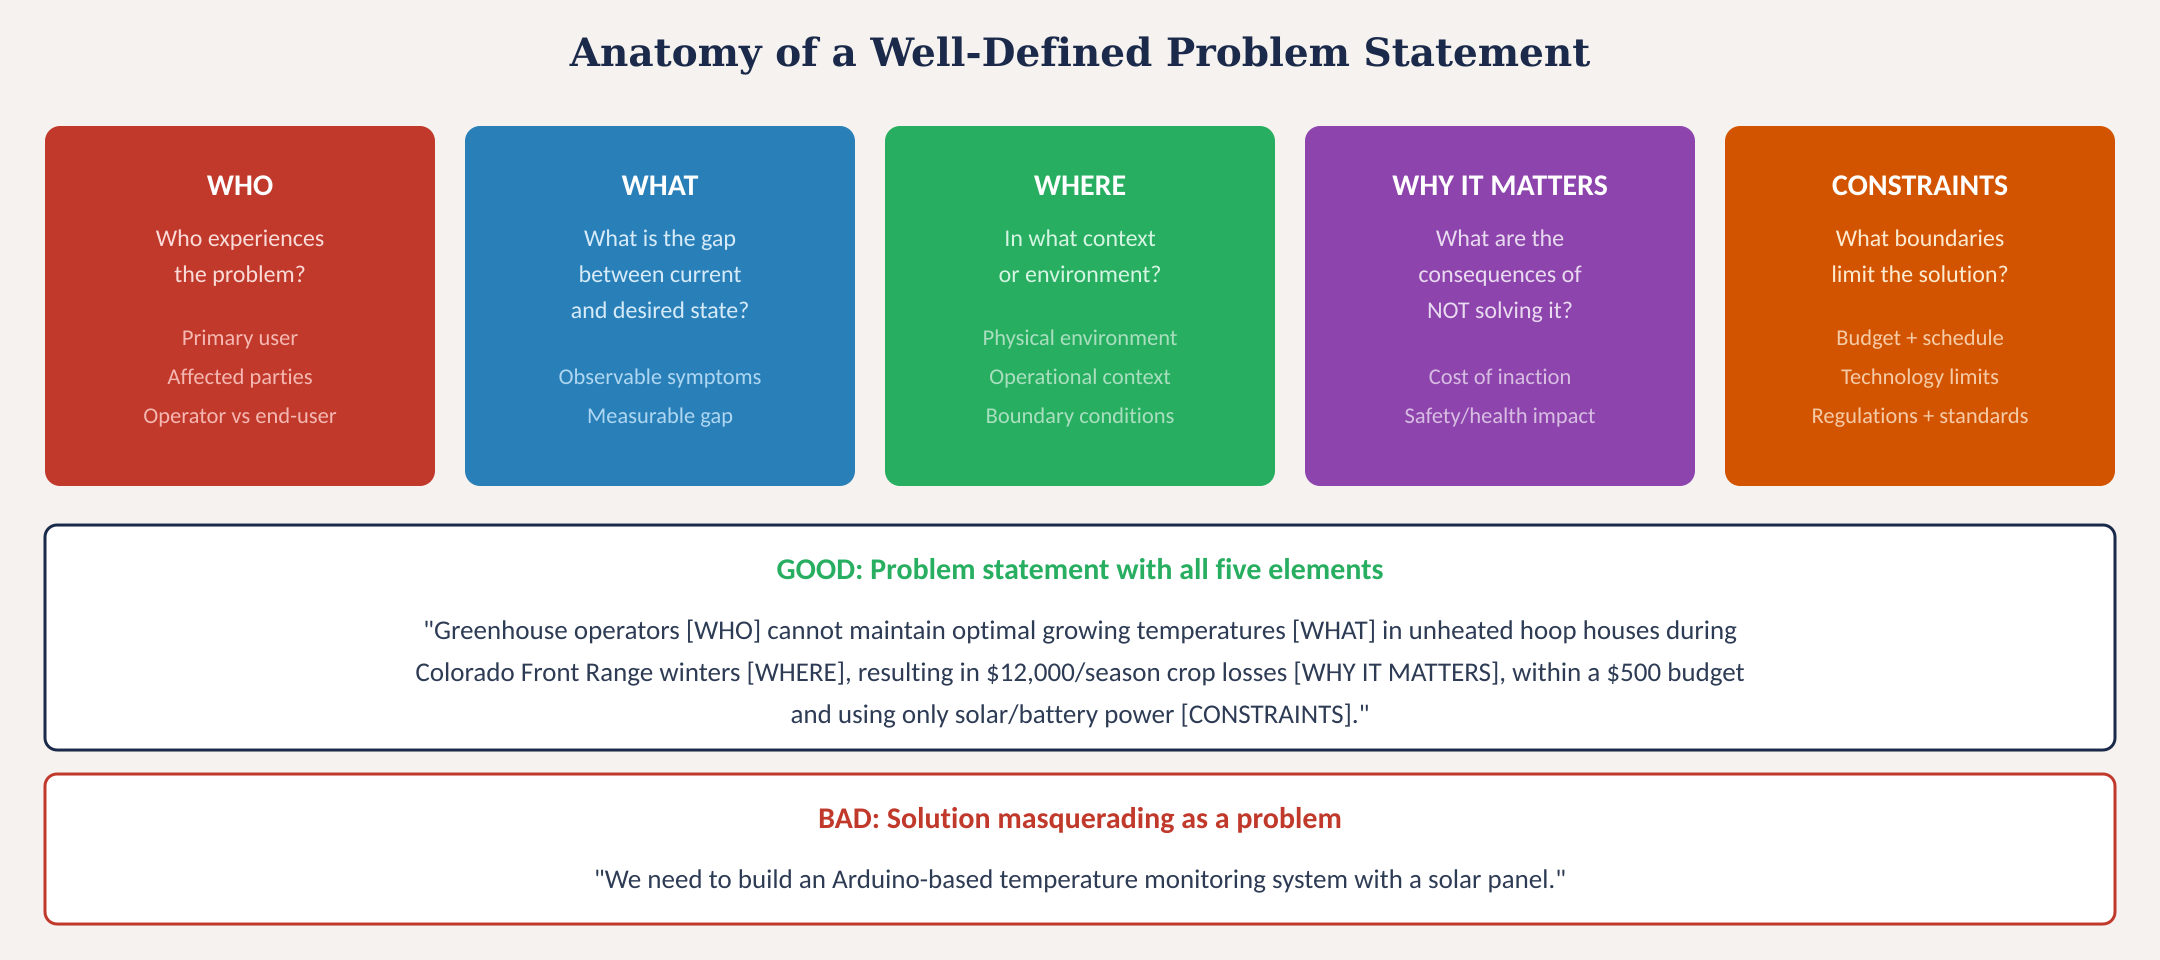
\includegraphics[width=\textwidth]{Problem Statement and Stakeholder Engagement/fig_problem_anatomy.png}
\caption{Five-element problem statement framework with good and bad examples.}\label{fig:prob}
\end{figure}

\begin{enumerate}[leftmargin=1.5em]
\item \textbf{WHO}: Who experiences the problem? Be specific about roles and context.
\item \textbf{WHAT}: What is the measurable gap between current and desired states?
\item \textbf{WHERE}: In what physical, operational, or environmental context?
\item \textbf{WHY IT MATTERS}: What are the consequences of not solving it? (Cost, safety, health.)
\item \textbf{CONSTRAINTS}: What boundaries limit the solution? (Budget, schedule, technology, regulations.)
\end{enumerate}

Constraints directly become non-functional requirements. The ``why it matters'' element justifies the project's existence.

\subsection{Scope and Boundaries}
\textbf{Scope} defines what is inside and outside the project. Without it, scope creep expands the project indefinitely. The \textbf{system boundary} distinguishes what you build from what the environment provides. Capture this in a \textbf{context diagram}: your system as a single block with all external interfaces (power, data, user, mechanical, environmental) labeled.

\FloatBarrier
\section{Stakeholder Engagement}
\subsection{Identifying Stakeholders}
A stakeholder is anyone who affects, is affected by, or has an interest in the project. \textbf{Missing a stakeholder = missing requirements = integration surprises.}

\begin{figure}[ht!]\centering
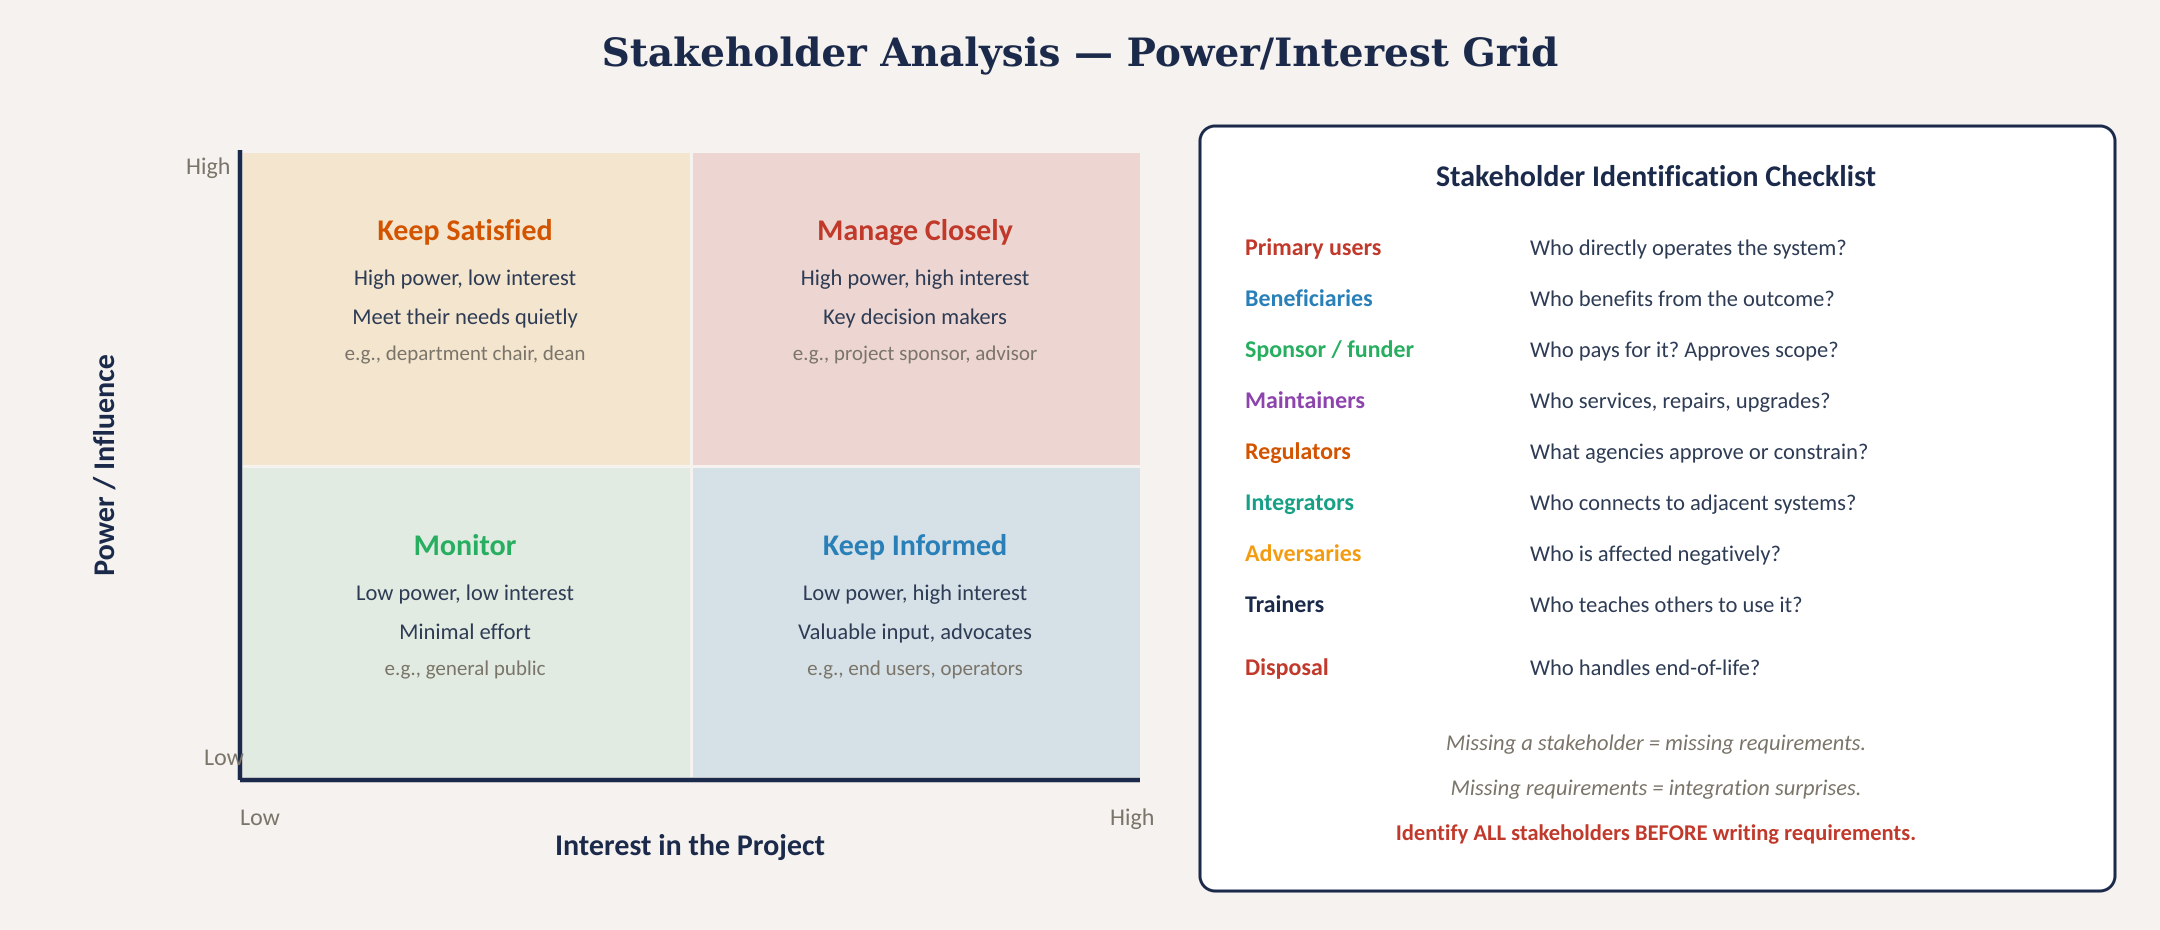
\includegraphics[width=\textwidth]{Problem Statement and Stakeholder Engagement/fig_stakeholder_grid.png}
\caption{Power/interest grid with engagement strategies and nine-category identification checklist.}\label{fig:stake}
\end{figure}

\textbf{Nine categories to check}: primary users, beneficiaries, sponsor/funder, maintainers, regulators, integrators (adjacent systems), adversaries, trainers, and disposal handlers. Students consistently miss maintainers, regulators, and adjacent-system owners.

\subsection{The Power/Interest Grid}
Classify each stakeholder by their power (ability to influence the project) and interest (how much they care). Four quadrants with distinct strategies: \textbf{Manage closely} (high power, high interest --- key decision makers), \textbf{Keep satisfied} (high power, low interest), \textbf{Keep informed} (low power, high interest --- valuable input), \textbf{Monitor} (low power, low interest).

\subsection{Needs Elicitation Techniques}

\begin{figure}[ht!]\centering
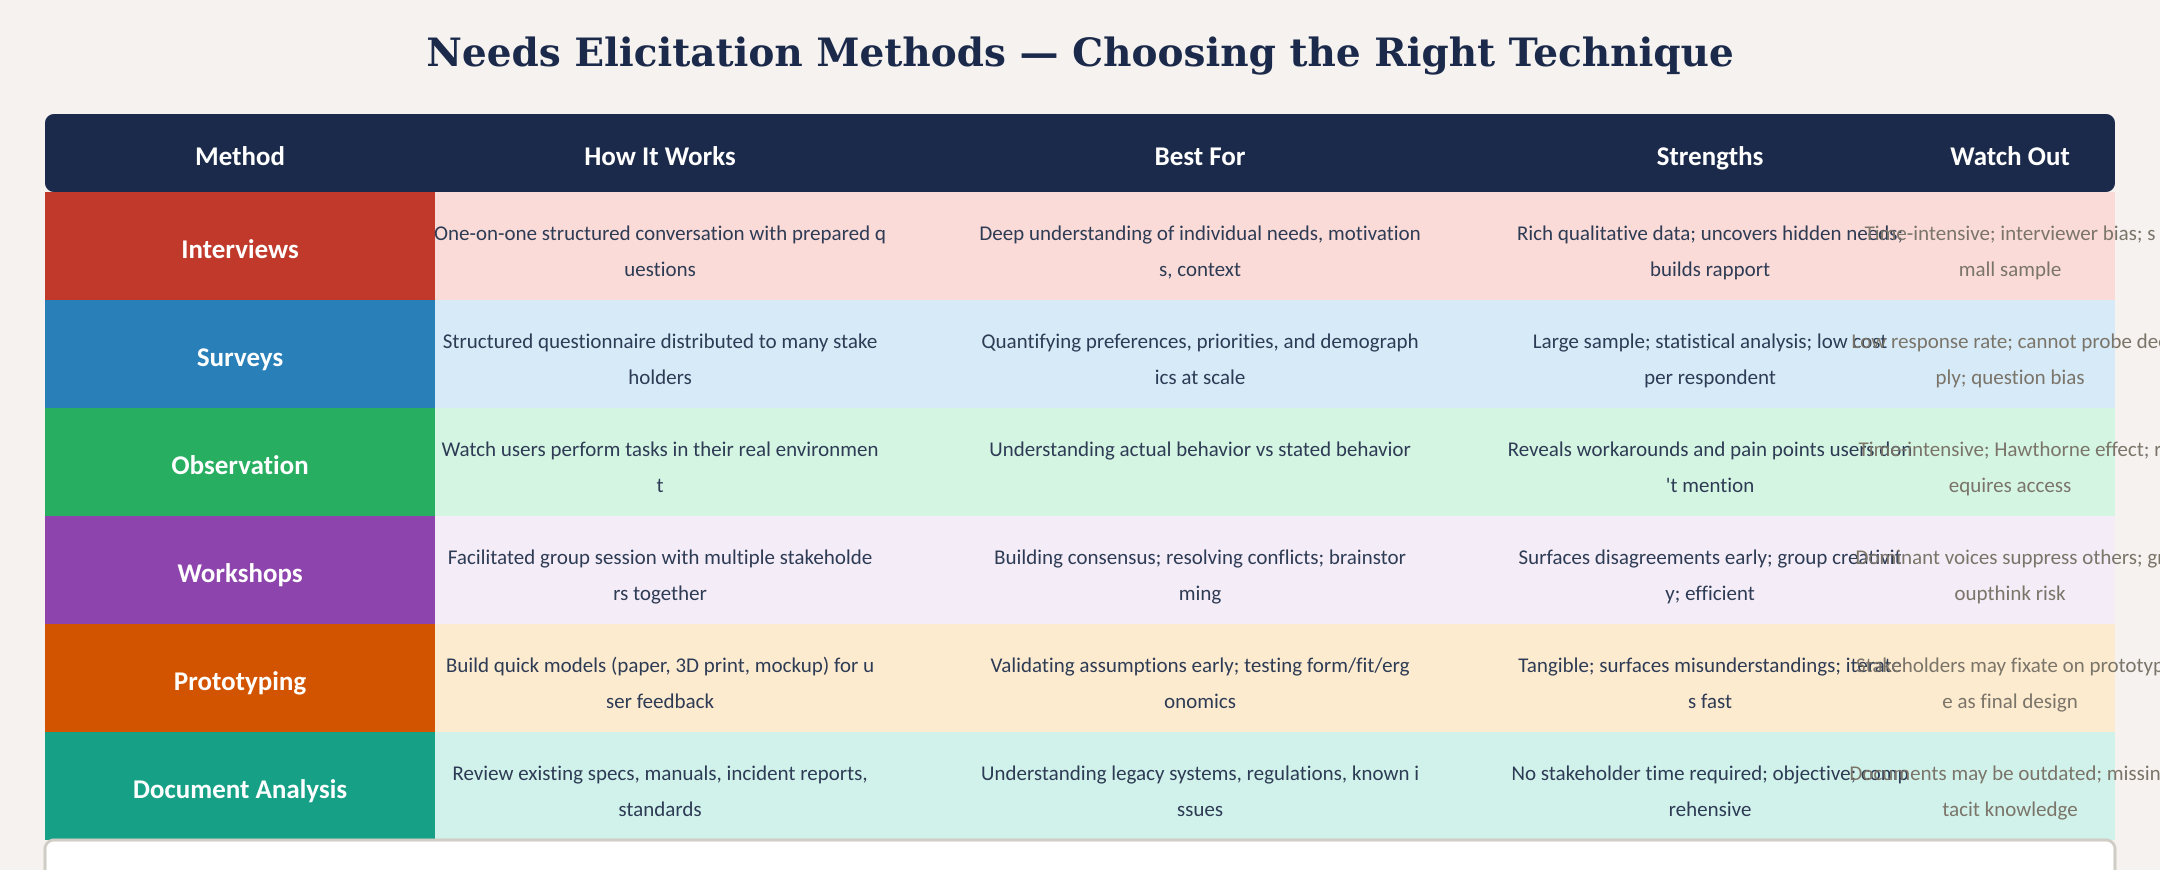
\includegraphics[width=\textwidth]{Problem Statement and Stakeholder Engagement/fig_elicitation_methods.png}
\caption{Six elicitation methods with best-use cases, strengths, and watch-outs.}\label{fig:elic}
\end{figure}

Use \textbf{2--3 methods} --- single-method elicitation misses needs. Strongest combination for engineering projects: \textbf{interviews} (capture stated needs) + \textbf{observation} (capture unstated needs) + \textbf{prototyping} (validate assumptions).

\needspace{4\baselineskip}
\begin{tipbox}[The Best Question in Engineering]
End every stakeholder interview with: ``What should I have asked that I didn't?'' This single question catches more missing requirements than any structured technique.
\end{tipbox}

\subsection{Managing Conflicting Needs}
Conflicts are normal. Prioritize using \textbf{MoSCoW}: Must (becomes SHALL), Should (becomes SHOULD), Could (if budget allows), Won't (explicitly excluded). When conflicts are irreconcilable, the sponsor or primary user has final authority --- but the decision must be documented. In MEGN~301, your section instructor acts as the key stakeholder and sponsor; they hold final authority on project-scope decisions when the team cannot resolve a conflict internally.

\subsection{Needs vs.\ Wants}
A \textbf{need} is something without which the system fails its mission --- it becomes a SHALL requirement. A \textbf{want} enhances value but the system works without it --- it becomes a SHOULD goal pursued only if resources allow. Separate them early.

\FloatBarrier
\section{From Problem to ConOps}
\subsection{Concept of Operations}
The Concept of Operations (ConOps) is the bridge between the problem statement and formal requirements. It describes how the system will be used from the stakeholder's perspective, written in \textbf{plain language} (no engineering jargon). The ConOps is not a design document; it is a stakeholder-facing narrative that captures the operational vision before any engineering decisions are made.

A complete ConOps addresses the following elements: (1)~the system mission and objectives, (2)~a description of the current situation and its deficiencies, (3)~operational scenarios covering normal, degraded, emergency, and maintenance modes, (4)~user roles and responsibilities, (5)~environmental and operating conditions, (6)~external interfaces and dependencies, and (7)~performance expectations expressed in stakeholder language.

The ConOps serves three critical functions in the SE lifecycle. First, it is the document the stakeholder reviews and approves \textbf{before requirements are written}---misunderstandings caught here cost minutes; caught in requirements, they cost weeks; caught in testing, they cost the project. Second, it provides the basis for validation: at the end of the project, you validate the system against the ConOps to confirm you solved the right problem. Third, it reveals implicit assumptions and unstated needs that interviews alone miss.

\needspace{4\baselineskip}
\begin{tipbox}[ConOps as a Contract]
Think of the ConOps as a contract between the engineering team and the stakeholder. The stakeholder says ``this is what I need the system to do in my world,'' and the engineering team says ``we will build something that operates this way.'' Once approved, changes to the ConOps require formal change control---just like changes to requirements.
\end{tipbox}

\subsection{Use Cases and Operational Scenarios}
A \textbf{use case} describes a specific user-system interaction to achieve a goal. It has a defined actor (the user or external system), a trigger (what initiates the interaction), a sequence of steps (the nominal flow), and a postcondition (what is true when the interaction succeeds). An \textbf{operational scenario} extends the use case into a realistic narrative with timing, weather, user state, and system state. Scenarios reveal requirements that abstract analysis misses.

\subsubsection{Writing Effective Use Cases}
Each use case should follow a structured format that makes the extraction of requirements systematic rather than ad hoc:

\begin{enumerate}[leftmargin=1.5em]
\item \textbf{Use Case ID and Name}: A unique identifier and descriptive title (e.g., UC-01: Automated Frost Response).
\item \textbf{Primary Actor}: The user role or external system that initiates the interaction.
\item \textbf{Preconditions}: What must be true before the use case can execute.
\item \textbf{Trigger}: The event that starts the use case.
\item \textbf{Nominal Flow}: The step-by-step sequence under normal conditions. Number each step. Write in present tense, active voice: ``The system detects\ldots'' ``The operator confirms\ldots''
\item \textbf{Alternative Flows}: Branches for degraded conditions, user errors, or edge cases. Reference the nominal step where they diverge.
\item \textbf{Postconditions}: What is true when the use case completes successfully.
\item \textbf{Exception Flows}: What happens when the use case cannot complete (sensor failure, communication loss, power failure).
\end{enumerate}

\subsubsection{From Use Cases to Requirements}
Each step in a use case implies one or more requirements. The extraction process is systematic: read each step, identify the capability the system must possess to execute that step, and write a SHALL statement. Preconditions generate interface and environmental requirements. Performance expectations embedded in the narrative (``within 30 seconds,'' ``at least twice daily'') become performance requirements. Exception flows generate reliability, redundancy, and graceful-degradation requirements.

\needspace{4\baselineskip}
\begin{keyconceptbox}[GreenShield: ConOps to Requirements Mapping]
\textbf{ConOps excerpt}: ``During normal overnight operation, when the air temperature inside the greenhouse drops below the user-defined frost threshold (default 3\,\degC), the system automatically activates the supplemental heater within 60 seconds and sends an SMS alert to the operator's mobile phone.''

\textbf{Derived requirements}:
\begin{itemize}[nosep]
\item SYS-REQ-01: The system shall monitor greenhouse air temperature continuously with a sample rate $\geq$ 1 reading per 60 seconds.
\item SYS-REQ-02: The system shall activate the supplemental heater when measured air temperature falls below the user-defined frost threshold.
\item SYS-REQ-03: The system shall complete heater activation within 60 seconds of detecting a below-threshold temperature reading.
\item SYS-REQ-04: The system shall transmit an SMS alert to the operator within 120 seconds of heater activation.
\item SYS-REQ-05: The system shall allow the operator to set the frost threshold between $-5$\,\degC\ and $+10$\,\degC\ in increments of 0.5\,\degC.
\end{itemize}
Notice how a single paragraph of stakeholder-facing narrative yields five formal, testable requirements. This is the power of the ConOps-to-requirements pipeline.
\end{keyconceptbox}

\begin{figure}[ht!]\centering
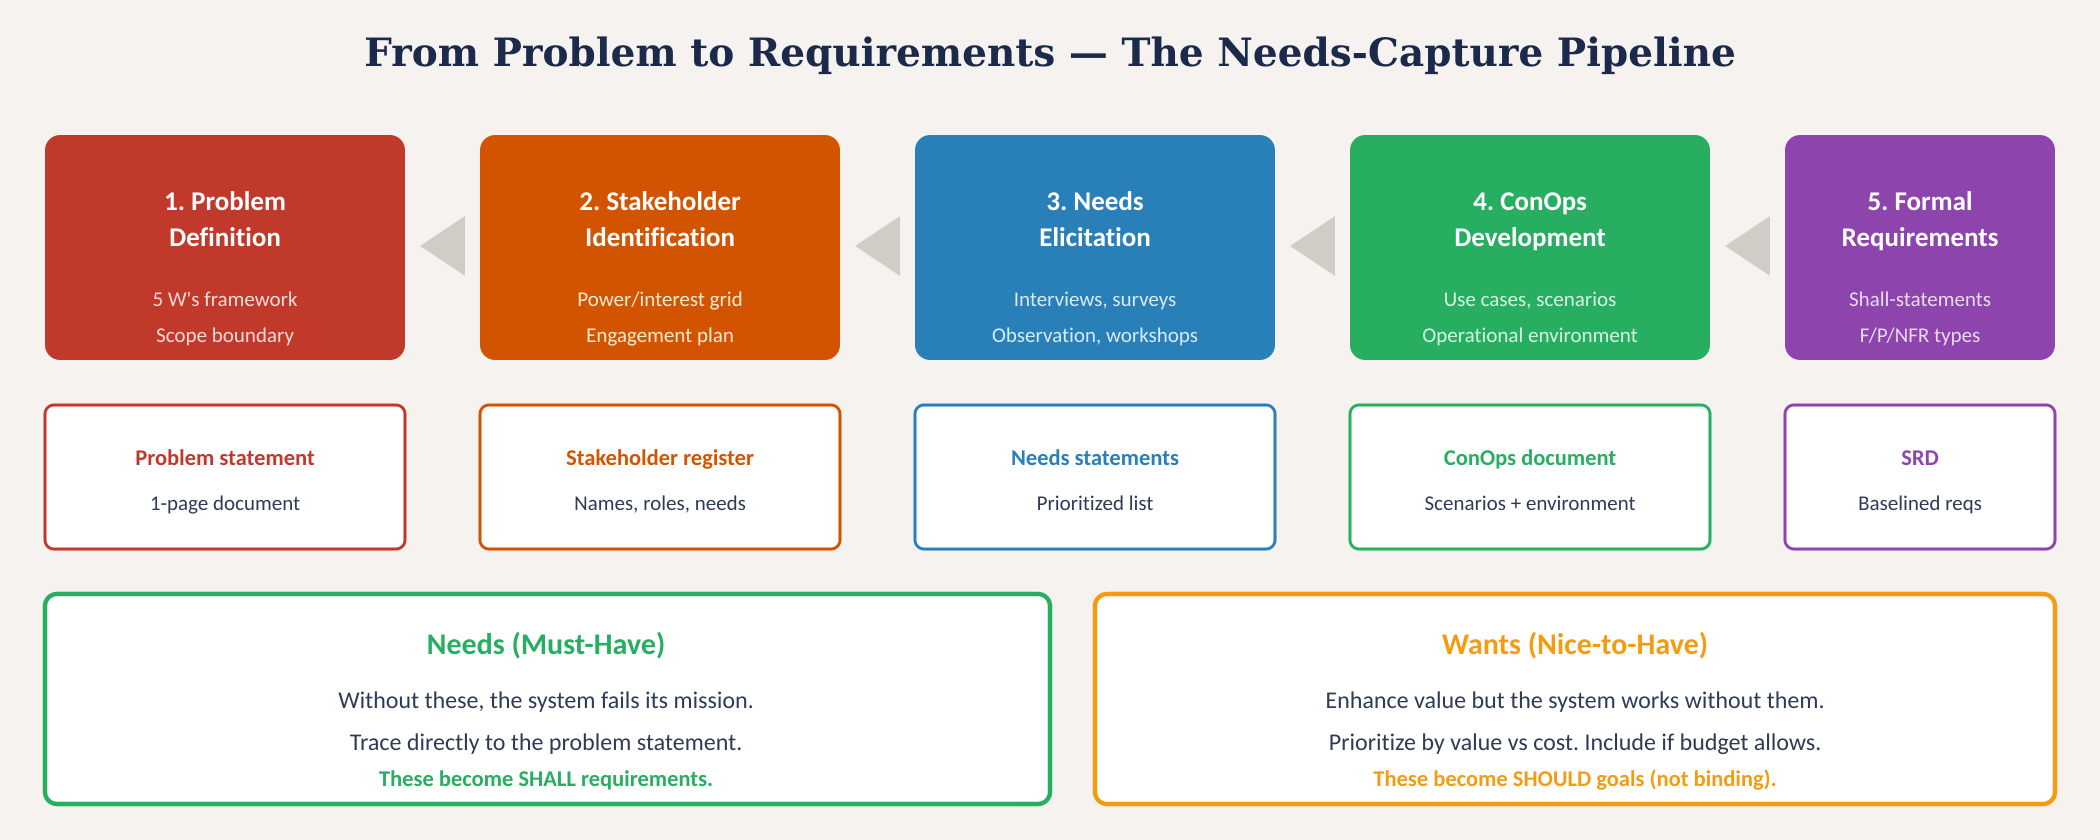
\includegraphics[width=\textwidth]{Problem Statement and Stakeholder Engagement/fig_needs_pipeline.png}
\caption{Five-stage needs-capture pipeline from problem to formal requirements with deliverables.}\label{fig:pipe}
\end{figure}

\FloatBarrier
\section{Artifact Handoff: What Chapter~1 Produces}

Every phase of the SE lifecycle produces artifacts that become inputs to the next phase. The following table summarizes the outputs of Chapter~1 and where they are consumed downstream.

\begin{center}
\small
\begin{tabularx}{\textwidth}{l X X}
\toprule
\textbf{Artifact from Ch.~1} & \textbf{Primary Contents} & \textbf{Used Directly In\ldots} \\
\midrule
Five-element problem statement & WHO / WHAT / WHERE / WHY / constraints & System-level requirements (Ch.~2); project justification \\
Stakeholder registry + power/interest grid & Roles, authority, engagement strategy & ConOps review, validation plan (Ch.~4), training plan (Ch.~6) \\
ConOps \& operational scenarios & Narratives, modes, performance expectations; \textbf{approved by section instructor (acting as sponsor)} & Requirements derivation (Ch.~2), test scenario design (Ch.~4), validation criteria \\
Use case descriptions & Actor-trigger-flow-postcondition & Functional requirements (Ch.~2), functional decomposition (Ch.~2) \\
Scope and boundary definition & Context diagram, system boundary & Architecture block diagrams (Ch.~2), ICD identification (Ch.~5) \\
\bottomrule
\end{tabularx}
\end{center}

\needspace{4\baselineskip}
\begin{tipbox}[Industry SE Parallels]
This chapter corresponds to INCOSE Systems Engineering Handbook Sections~4.1--4.3 (Stakeholder Needs Definition, Requirements Analysis initial steps) and NASA SP-2016-6105 Rev~2, Chapter~4.1 (Stakeholder Expectations Definition). In industry, the ConOps is often a formal deliverable reviewed at a System Requirements Review (SRR), which precedes the Preliminary Design Review. The MoSCoW prioritization method maps to what INCOSE calls ``needs prioritization and conflict resolution'' within stakeholder engagement.
\end{tipbox}

\FloatBarrier
\section{Practice Questions}
Questions are tiered: \textbf{C} = Comprehension, \textbf{A} = Application, \textbf{CT} = Critical Thinking.
\begin{enumerate}[leftmargin=1.5em]
\item \textbf{[C]} Rewrite this solution-as-problem into a proper five-element problem statement: ``We need to design a solar-powered weather station using a Raspberry Pi.''
\item \textbf{[C]} List all stakeholders for a senior capstone project that designs an automated pet feeder for elderly users. Use the nine-category checklist.
\item \textbf{[A]} You interview a greenhouse operator who says ``I need a temperature display.'' Through observation, you notice she checks the display, then walks to the heater and turns it on manually. What is her \emph{actual} need? How does this change the requirements?
\item \textbf{[A]} Classify these stakeholders on a power/interest grid for a campus parking management system: (a) university president, (b) daily commuter student, (c) campus police, (d) city traffic department, (e) disability services office.
\item \textbf{[CT]} Write a 1-paragraph ConOps for an automated frost protection system for a small greenhouse, including at least two operational scenarios (normal and degraded mode).
\item \textbf{[CT]} A sponsor wants the system under \$500, the user wants a touchscreen display, and the maintainer wants modular components. These conflict. How do you resolve this using the MoSCoW framework?
\end{enumerate}

\subsection{Answers}
\begin{enumerate}[leftmargin=1.5em]
\item ``Small-farm operators [WHO] lack access to real-time, site-specific weather data [WHAT] at remote agricultural locations without grid power [WHERE], leading to crop management decisions based on regional forecasts that miss micro-climate variations by up to 5\,$^{\circ}$ C [WHY], within a \$300 budget using only renewable power sources [CONSTRAINTS].''
\item Primary users: elderly pet owner (operator). Beneficiaries: the pet; family members who worry remotely. Sponsor: the pet owner or their family. Maintainers: family member or home-care aide who refills food and troubleshoots. Regulators: food-safety standards for pet food storage; electrical safety (UL). Integrators: home Wi-Fi network; smartphone (if app-connected). Adversaries: the pet (may try to defeat the mechanism). Trainers: whoever teaches the elderly user. Disposal: recycling or trash service.
\item Her actual need is automated frost protection, not a temperature display. The display is her current workaround for a lack of automation. The real requirement is: ``The system shall activate the supplemental heater when temperature drops below a user-defined setpoint.'' The display becomes a secondary want, not the primary need. This changes the architecture from a passive monitor to an active control system.
\item (a) University president: high power, low interest $\to$ Keep Satisfied. (b) Commuter student: low power, high interest $\to$ Keep Informed. (c) Campus police: high power, high interest $\to$ Manage Closely (they enforce parking rules). (d) City traffic department: moderate power, low interest $\to$ Keep Satisfied (jurisdiction over surrounding roads). (e) Disability services: moderate power, high interest $\to$ Manage Closely (ADA compliance is non-negotiable).
\item ``The frost protection system monitors greenhouse air temperature continuously. During normal operation, when temperature drops below the user-defined threshold (default 3\,$^{\circ}$ C), the system automatically activates the supplemental heater and sends an alert to the operator's phone. The operator can acknowledge the alert, adjust the setpoint, or override the system remotely. In degraded mode (communication failure), the system continues autonomous control using local logic, activating the heater based on its last-known setpoint and logging events locally until communication is restored. The operator discovers the communication failure on their next manual check or when they notice the absence of the daily status report.''
\item MoSCoW: \textbf{Must}: system cost under \$500 (sponsor constraint --- non-negotiable). Modular components for field replacement (maintainer need --- essential for long-term usability). \textbf{Should}: visual status display (user need --- but a low-cost LCD or LED indicators at \$5 may satisfy the need without a \$50 touchscreen). \textbf{Could}: touchscreen interface (user want --- only if budget allows after must-haves). \textbf{Won't}: full-color graphical touchscreen in v1.0. Resolution: the display is a legitimate need but the \emph{touchscreen} is a want. Propose a 2-line LCD (\$3) for v1.0 with a touchscreen upgrade path for v2.0 if the sponsor increases budget.
\end{enumerate}

\FloatBarrier
\chapter{Writing Requirements \& Defining Architecture}

\vspace{1em}

This chapter covers the middle-left of the V-Model: translating the stakeholder's needs and ConOps (Chapter~1) into formal, testable requirements, and then decomposing those requirements into a system architecture with defined functions, subsystems, and interfaces. Requirements are the single most important artifact in systems engineering---they define the contract between what the stakeholder needs and what the engineering team builds, and they establish the criteria against which every verification test (Chapter~4) is judged. Architecture defines \emph{how} the system is organized to satisfy those requirements.

\needspace{4\baselineskip}
\begin{keyconceptbox}[Bottom Line]
Transform stakeholder needs into numbered, testable SHALL statements organized in an RTM. Then decompose those requirements into functions (what the system does) before choosing components (how it does it). Your SDRD and architecture block diagram are the two artifacts that define your project's scope---everything downstream flows from them.
\end{keyconceptbox}

\vspace{1em}

\FloatBarrier
\section{Writing Requirements}
\subsection{The System Design Requirements Document (SDRD)}
In MEGN~301, your requirements are captured in a \textbf{System Design Requirements Document (SDRD)}, which uses a three-level hierarchy:

\textbf{Level 1: Goal Statement.} One or two sentences that capture the system's mission and purpose in ``big picture'' terms. The goal statement presents the system function with meaningful context regarding the overall mission and underlying motivations. Example: ``Design an automated frost protection system that enables small-scale greenhouse operators to prevent crop loss during overnight frost events without manual intervention.''

\textbf{Level 2: Objectives.} Qualitative statements of what the design needs to be able to do or look like in order to achieve the goal. Objectives flesh out the goal statement and span the entire function of the system. They are complete, clear, and solution-agnostic. Example: ``The system shall monitor greenhouse environmental conditions and automatically activate heating when frost is imminent.''

\textbf{Level 3: Design Requirements.} Quantitative, measurable, testable statements that precisely describe the capabilities or constraints needed to fulfill each objective. Every design requirement must be clear, precise, quantifiable, and measurable. Requirements are organized under their parent objective. Example: ``SYS-REQ-01: The system shall measure ambient air temperature with accuracy $\leq \pm 0.5$\,\degC\ over $-10$ to $+50$\,\degC.''

This Goal $\to$ Objectives $\to$ Requirements hierarchy maps directly to the SE hierarchy discussed below: the Goal corresponds to the system mission (ConOps), Objectives correspond to stakeholder needs, and Design Requirements correspond to formal SHALL statements with verification methods.

\needspace{4\baselineskip}
\begin{warningbox}[Requirements Are Testable Contracts]
The SDRD is a contract between your team and the customer (your instructor). You will be tested against these requirements. If a requirement cannot be tested, it cannot be verified, and your project's success cannot be demonstrated. Every requirement in your SDRD must have a corresponding test in your Test Plan (Chapter~4). Write them in parallel.
\end{warningbox}

\subsection{What Is a Requirement?}
A requirement is a formal statement of a capability or constraint the system must satisfy. It uses the word \textbf{shall} to indicate mandatory compliance. ``The system \emph{shall} measure ambient temperature'' is a requirement. ``Should'' and ``will'' are non-binding.

A well-formed requirement has: (1) a unique ID (SYS-REQ-042) for traceability, (2) a single shall-statement with one testable condition, (3) measurable acceptance criteria with units and tolerance, (4) a rationale explaining why it exists, and (5) a verification method (Test, Analysis, Inspection, or Demonstration).

\needspace{4\baselineskip}
\begin{warningbox}[Common Failures]
\textbf{Vague}: ``shall be fast.'' \textbf{Compound}: ``shall measure AND display.'' \textbf{Untestable}: ``shall be user-friendly.'' \textbf{Gold-plated}: ``shall use an Arduino'' (specifies implementation, not need). Each failure produces downstream rework.

Compound requirements deserve special attention: ``The system shall measure and display ambient temperature'' looks innocent but creates a traceability nightmare. If the sensor works but the display is broken, does the requirement PASS or FAIL? You cannot assign a single TAID method because measuring requires Test (calibrated reference) while displaying requires Inspection (visual check). Split it into two requirements, each with its own test. One compound requirement in the SDRD can cascade into untestable verification at FDR.
\end{warningbox}

\subsection{Requirement Types}
\begin{itemize}[leftmargin=1.5em]
\item \textbf{Functional}: What the system shall \emph{do}. Actions: sense, compute, transmit, actuate, display. ``The system shall measure ambient temperature.''
\item \textbf{Performance}: How \emph{well} it does it. Quantitative criteria. ``\ldots with accuracy of $\pm 0.5$\,$^{\circ}$ C over $-20$ to $+60$\,$^{\circ}$ C at $\geq$1\,Hz.'' A functional requirement without a paired performance requirement is incomplete.
\item \textbf{Non-Functional (NFR)}: Constraints on \emph{how} it is built. Environmental (``operate at $-20$ to $+60$\,$^{\circ}$ C''), regulatory (``comply with FCC Part 15''), material (``RoHS-compliant''), reliability (``$\geq$1000 hrs MTBF''), interface (``CAN 2.0B'').
\end{itemize}

\subsection{Requirements Hierarchy and Traceability}
Requirements decompose top-down: stakeholder needs $\to$ system requirements $\to$ subsystem requirements $\to$ component specifications. Each level adds detail and specificity. Every child requirement traces to a parent (backward traceability). Every parent is decomposed into children (forward traceability). An orphan requirement has no justification; an undecomposed requirement has no implementation.

This hierarchy is not merely organizational---it is the mechanism that ensures completeness and prevents both gold-plating (building features no one asked for) and gaps (failing to implement a need). When you add a requirement at any level, you must be able to answer two questions: (1)~What parent need justifies this requirement? (backward trace), and (2)~How will this requirement be allocated to subsystems or components? (forward trace).

\begin{figure}[ht!]\centering
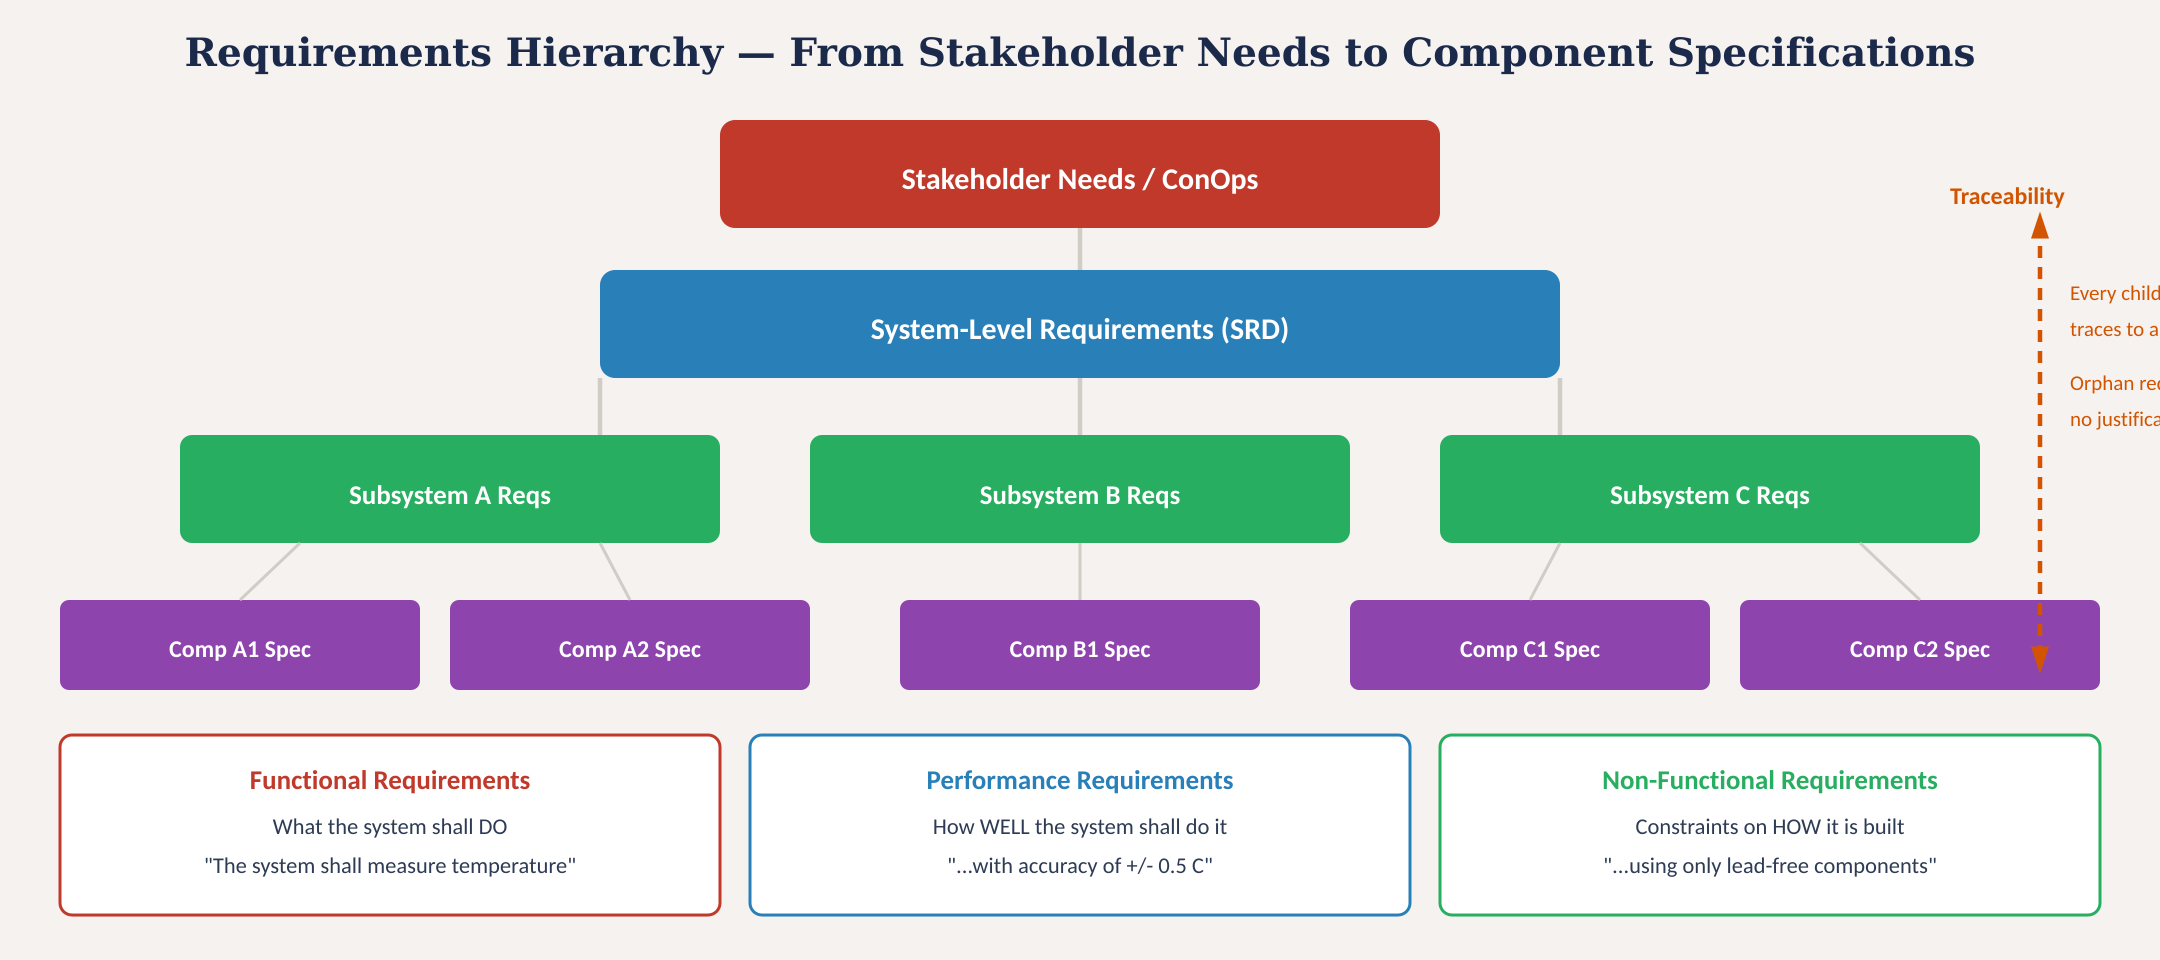
\includegraphics[width=\textwidth]{Requirements and Architecture/fig_req_hierarchy.png}
\caption{Requirements hierarchy from stakeholder needs through system, subsystem, and component levels with traceability and three requirement types.}\label{fig:hier}
\end{figure}

\subsubsection{The Requirements Traceability Matrix (RTM)}
The Requirements Traceability Matrix is the bookkeeping tool that implements bidirectional traceability. It is a living document maintained from the moment you write your first requirement through final delivery. The RTM links every requirement to its parent need, its child allocations, its verification method, and its current verification status.

A minimal RTM for a student project contains the following columns:

\begin{center}
\small
\begin{tabularx}{\textwidth}{l l X l l l}
\toprule
\textbf{Req ID} & \textbf{Parent} & \textbf{Requirement Text} & \textbf{Type} & \textbf{V-Method} & \textbf{Status} \\
\midrule
SN-01 & --- & Operator needs automated frost protection & Need & --- & --- \\
SYS-01 & SN-01 & Shall monitor air temp continuously ($\geq$1/min) & Func & T & Verified \\
SYS-02 & SN-01 & Shall activate heater when $T < T_{\text{set}}$ & Func & T & Verified \\
SYS-03 & SN-01 & Shall complete activation within 60\,s & Perf & T & Open \\
SS-01a & SYS-01 & Sensor accuracy $\leq \pm 0.5$\,\degC & Perf & T & Verified \\
SS-01b & SYS-01 & ADC resolution $\leq 0.1$\,\degC & Perf & A & Verified \\
\bottomrule
\end{tabularx}
\end{center}

The RTM evolves as the project progresses. Before PDR, the ``Status'' column is mostly ``Open.'' By CDR, subsystem requirements should be allocated and verification methods assigned. By FDR, every row should show ``Verified,'' ``Waived,'' or ``Deferred with plan.'' The RTM is the single artifact that tells the complete project story at any point in time.

\needspace{4\baselineskip}
\begin{warningbox}[RTM Discipline: Your Central Nervous System]
A mature engineering team uses the RTM as its central nervous system---the \emph{first} document opened at every team meeting and the \emph{last} document updated after every design decision. Your goal is to reach that level of proficiency this semester. If a requirement cannot be traced to a need, delete it. If a need has no requirement, write one. If a requirement has no verification method, it is untestable---rewrite it. The RTM is not a box to check before a review; it is the living document that tells you whether your project is on track at any moment.
\end{warningbox}

\subsubsection{Requirements Documentation Template}
Each requirement should be documented with five elements to ensure it is complete, traceable, and verifiable:

\begin{center}
\small
\begin{tabularx}{\textwidth}{l X}
\toprule
\textbf{Field} & \textbf{Description and Example} \\
\midrule
\textbf{ID} & Unique identifier with hierarchical prefix. \emph{SYS-REQ-003} \\
\textbf{Text} & Single SHALL statement with quantitative criteria. \emph{The system shall measure ambient temperature with accuracy $\leq \pm 0.5$\,\degC\ over 0 to 50\,\degC.} \\
\textbf{Rationale} & Why this requirement exists; traces to the parent need. \emph{Derived from SN-01: operator requires temperature monitoring to prevent frost damage.} \\
\textbf{Verification Method} & T, A, I, or D (from TAID---see Ch.~4). \emph{Test: calibrated reference bath comparison at 6 temperature points.} \\
\textbf{Parent ID} & The stakeholder need or parent requirement from which this is derived. \emph{SN-01} \\
\bottomrule
\end{tabularx}
\end{center}

\subsection{Writing Good Requirements --- Five Rules}
\begin{enumerate}[leftmargin=1.5em]
\item \textbf{One shall per requirement}: compound requirements are untestable.
\item \textbf{Quantitative criteria}: numbers, units, tolerance. ``Fast'' is not a requirement.
\item \textbf{Testable as written}: if you cannot envision a test procedure, rewrite.
\item \textbf{Implementation-free}: state WHAT, not HOW. ``$\geq$12 analog inputs'' not ``use Arduino Mega.''
\item \textbf{Include rationale}: WHY does this requirement exist? Prevents zombie requirements.
\end{enumerate}

\FloatBarrier
\section{Defining Architecture}
\subsection{Functional Decomposition}
Define WHAT the system must do (functions) before deciding HOW (physical components). This separation is the most important conceptual discipline in systems engineering. Functions are stable across implementations---``Sense Temperature'' remains the same function whether you implement it with a thermocouple, RTD, or infrared sensor. Implementations change; functions persist.

Break the system mission into primary functions, sub-functions, and leaf functions. Each leaf function maps to a physical component or module. Use verb-noun naming: Sense Temperature, Process Data, Provide Power, Actuate Heater. The functional decomposition tree is the skeleton upon which the entire architecture hangs.

\begin{figure}[ht!]\centering
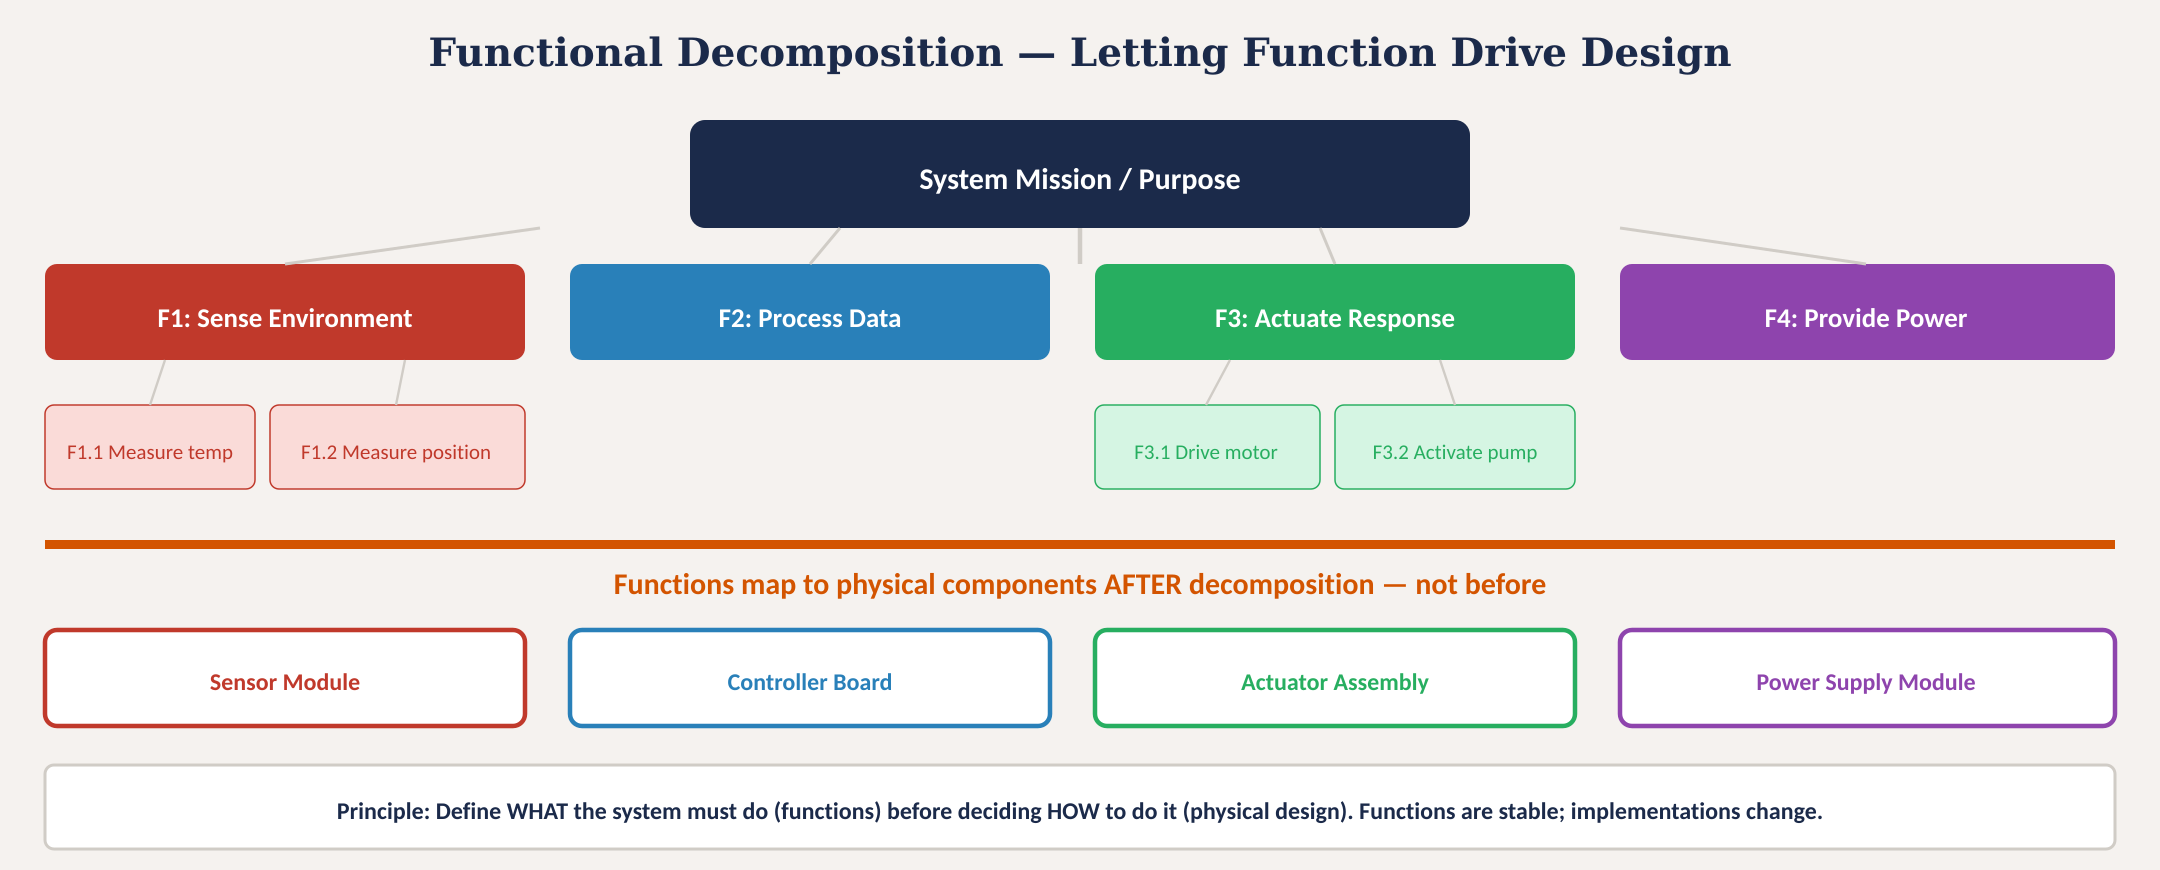
\includegraphics[width=\textwidth]{Requirements and Architecture/fig_functional_decomp.png}
\caption{Functional decomposition: functions defined before physical allocation. Functions are stable; implementations change.}\label{fig:func}
\end{figure}

\needspace{4\baselineskip}
\begin{keyconceptbox}[GreenShield: Functional Decomposition]
Starting from the system requirements derived in Chapter~1, the GreenShield frost protection system decomposes into these primary functions:

\begin{enumerate}[nosep]
\item \textbf{Sense Environment}: Monitor air temperature, detect threshold crossings.
\item \textbf{Process \& Decide}: Compare measurements to setpoint, execute control logic, log data.
\item \textbf{Actuate Heater}: Switch supplemental heater on/off via relay or contactor.
\item \textbf{Communicate}: Send alerts to operator, receive remote commands.
\item \textbf{Provide Power}: Supply regulated power to all subsystems from mains or backup.
\item \textbf{Interface with Operator}: Accept setpoint input, display status.
\end{enumerate}

Each primary function decomposes further. For example, ``Sense Environment'' decomposes into: (a)~Transduce temperature to electrical signal, (b)~Condition signal (amplify, filter), (c)~Digitize signal (ADC), and (d)~Validate reading (range check, noise rejection). Each leaf function will eventually be allocated to a physical component during concept selection (Chapter~3).
\end{keyconceptbox}

\subsection{From Functions to Architecture Blocks}
Once the functional decomposition is complete, group related leaf functions into \textbf{subsystems} (also called modules or blocks). This grouping is a design decision---there is no single correct answer, and the choice of grouping defines the system architecture. Good groupings minimize the number and complexity of inter-subsystem interfaces, because interfaces are where integration failures occur (Chapter~5).

Present the architecture as a \textbf{block diagram}: each subsystem is a labeled box, and every interface between boxes is a labeled arrow showing what crosses the boundary (signals, power, data, mechanical coupling, fluid flow). The block diagram, combined with the Interface Control Documents, is the architecture definition.

\subsubsection{Worked Example: GreenShield Architecture}
Grouping the GreenShield functions into subsystems yields the following architecture:

\begin{center}
\small
\begin{tabularx}{\textwidth}{l X X}
\toprule
\textbf{Subsystem} & \textbf{Allocated Functions} & \textbf{Key Requirements Allocated} \\
\midrule
Sensor Module & Transduce, condition, digitize temperature & SYS-01, SS-01a, SS-01b \\
Controller & Process, decide, log, validate readings & SYS-02, SYS-03, SYS-05 \\
Power Relay Module & Switch heater, provide electrical isolation & SYS-02, SYS-03, safety NFRs \\
Communication Module & SMS alerts, remote command reception & SYS-04 \\
Power Supply & Regulate mains power, distribute to subsystems & Power NFRs, environmental NFRs \\
Operator Interface & Setpoint input, status display & SYS-05, usability NFRs \\
\bottomrule
\end{tabularx}
\end{center}

The interfaces between these subsystems are: Sensor $\to$ Controller (I$^2$C digital temperature data), Controller $\to$ Relay (GPIO digital control signal), Controller $\to$ Comm (UART serial data), Power $\to$ All (regulated 5V/3.3V DC rails), Operator $\to$ Controller (button inputs, LCD data bus).

\subsection{Interface Definition}
Once functions map to modules, define interfaces between them with Interface Control Documents (ICDs): what crosses the boundary (signals, power, data, fluid), in what format (protocols, voltage levels, connector types), with what constraints (bandwidth, latency, current limits, pressure ratings).

Each interface should have a single \textbf{owner}---the person or sub-team responsible for ensuring both sides of the interface are compatible. In practice, interface ownership is assigned to the subsystem that \emph{provides} the signal or resource. See Part~II (Connectors chapter) for detailed guidance on specifying electrical ICD parameters.

An ICD for an electrical interface should specify, at minimum: (1)~connector type and part number, (2)~pinout with signal names, (3)~voltage levels and logic family, (4)~signaling protocol and data rate, (5)~maximum current per pin, (6)~grounding and shielding requirements, and (7)~cable length constraints.

\subsection{Architecture Patterns}
\textbf{Centralized}: one controller manages all subsystems. Simple to implement, easy to debug, but creates a single point of failure. Best for small systems with few subsystems and low reliability requirements. \textbf{Distributed}: multiple controllers communicate on a shared bus (CAN, I$^2$C, SPI). More robust---a failure in one node does not necessarily disable others. Enables parallel development by different sub-teams. More complex to integrate and debug. \textbf{Hierarchical}: layered control with a supervisory controller coordinating subordinate controllers. Combines the advantages of centralized (clear authority) and distributed (local autonomy). Common in automotive and aerospace systems.

Choose based on reliability requirements, system complexity, team structure, and interface complexity. For most MEGN~301 projects, a centralized architecture with a single microcontroller is appropriate.

\subsection{Requirements--Architecture Iteration}
In practice, requirements and architecture are not developed sequentially---they co-evolve through iteration. As you develop the architecture, you discover feasibility constraints, cost implications, and interface complexities that may require revising requirements. For example, you may discover that achieving $\pm 0.5$\,\degC\ accuracy requires a \$45 sensor that blows the budget, and the stakeholder agrees to relax the requirement to $\pm 1.0$\,\degC.

This iteration is normal and healthy, but it must be \textbf{formally controlled}. Any change to a baselined requirement requires: (1)~a change request documenting the proposed change and its rationale, (2)~an impact assessment on all downstream artifacts (architecture, tests, schedule, cost), (3)~stakeholder approval, and (4)~updates to the RTM and all affected documents. Never silently change a requirement---this destroys traceability and creates ``ghost'' failures during verification.

\begin{figure}[ht!]\centering
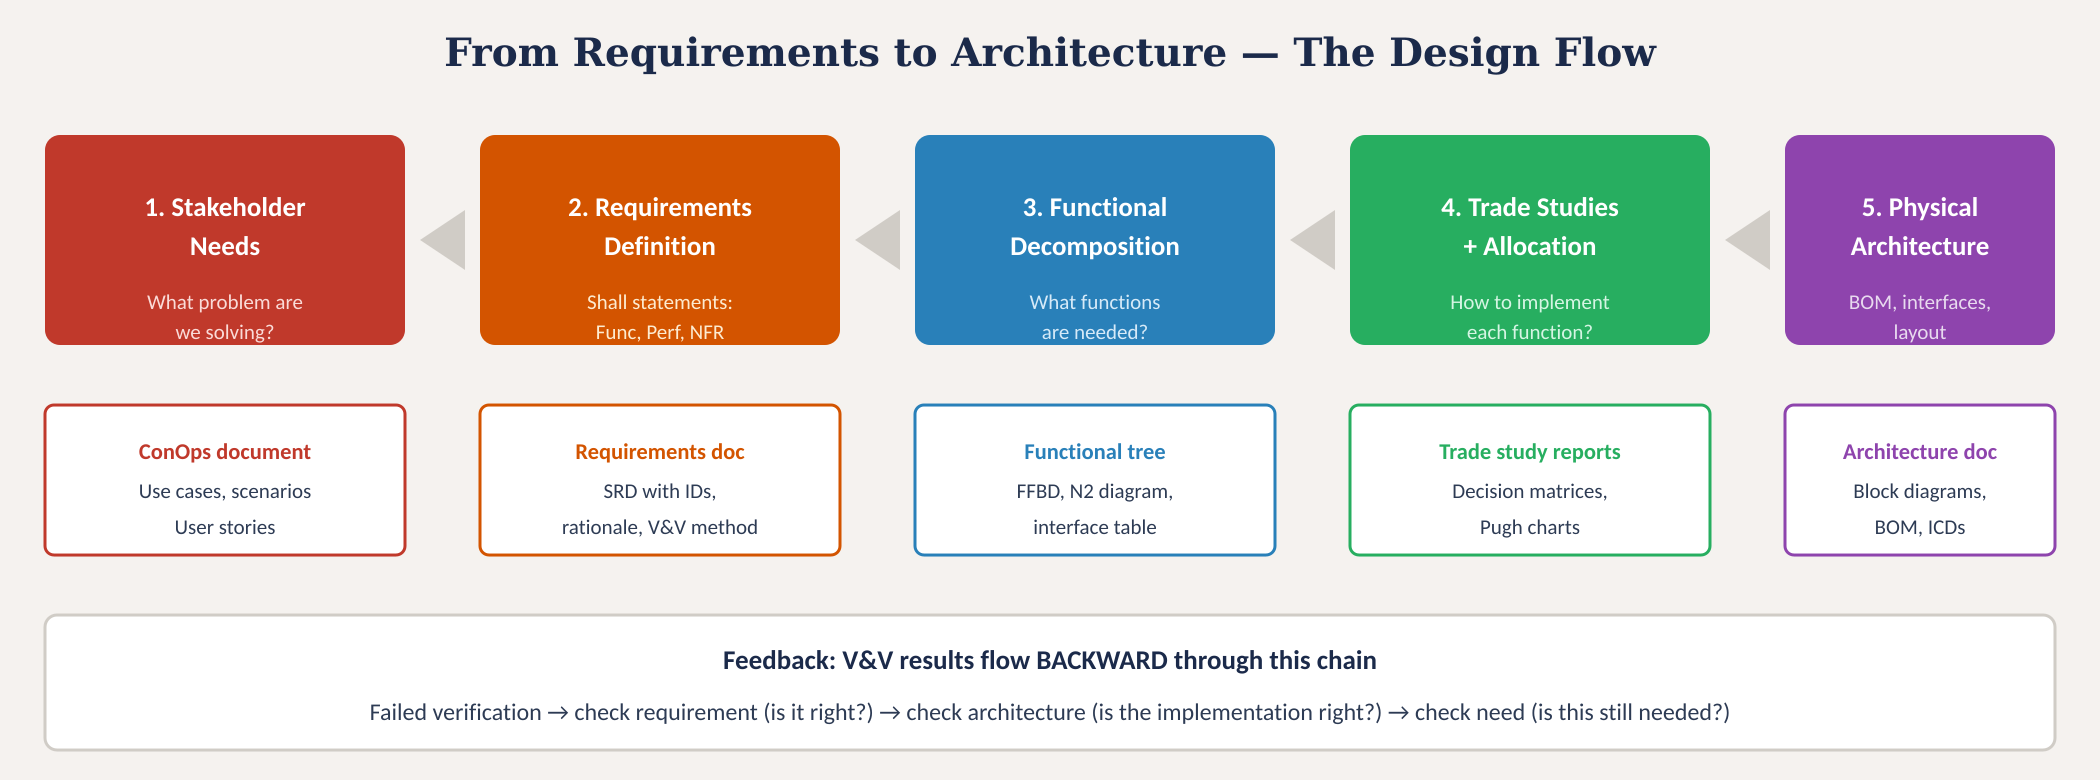
\includegraphics[width=\textwidth]{Requirements and Architecture/fig_design_flow.png}
\caption{Five-stage design flow: stakeholder needs $\to$ requirements $\to$ functional decomposition $\to$ architecture allocation $\to$ interface definition. Arrows flow both directions as architecture insights feed back to refine requirements.}\label{fig:flow}
\end{figure}

\FloatBarrier
\section{Defining Environmental and Regulatory Constraints}
Environmental and regulatory requirements deserve special attention because they are often the most technically constraining and the most commonly overlooked by student teams.

\textbf{Environmental constraints} define the conditions under which the system must operate and survive. They include: operating temperature range (the range during active use), storage temperature range (often wider), humidity, vibration and shock profiles, altitude, solar radiation and UV exposure, dust and water ingress (IP ratings), and corrosive atmospheres. Each environmental condition generates at least one requirement, and each requirement must specify both the condition and the performance expected under that condition.

\textbf{Regulatory constraints} are non-negotiable. They include: electrical safety (UL, CE marking, NRTL), electromagnetic compatibility (FCC Part 15, CISPR), material restrictions (RoHS, REACH), sector-specific standards (FDA, USDA, OSHA), and accessibility requirements (ADA). Identify applicable regulations during stakeholder analysis (Chapter~1) and write them as non-functional requirements with specific standard references.

\needspace{4\baselineskip}
\begin{warningbox}[Environmental Requirements Are Testable]
``The system shall work outdoors'' is not a requirement. ``The system shall operate continuously at ambient temperatures from $-20$ to $+60$\,\degC\ with relative humidity up to 95\% non-condensing'' is a requirement---and it is testable (environmental chamber, Ch.~4). Define the envelope; test the boundaries.
\end{warningbox}

\FloatBarrier
\section{Artifact Handoff: What Chapter~2 Produces}

\begin{center}
\small
\begin{tabularx}{\textwidth}{l X X}
\toprule
\textbf{Artifact from Ch.~2} & \textbf{Primary Contents} & \textbf{Used Directly In\ldots} \\
\midrule
Requirements document & Numbered SHALL statements with types, rationale, V-method & Concept evaluation criteria (Ch.~3), test plans (Ch.~4), VCRM (Ch.~4) \\
RTM (initial) & Req IDs, parent traces, allocated V-methods, status (Open) & Maintained through Ch.~3--6; final version presented at FDR \\
Functional decomposition tree & Verb-noun function hierarchy & Morphological chart rows (Ch.~3), architecture allocation \\
Architecture block diagram & Subsystem blocks with labeled interfaces & Integration planning (Ch.~5), ICD development \\
Interface definitions / ICDs & Signal types, protocols, connectors, constraints & Integration testing (Ch.~5), connector selection (Part~II) \\
\bottomrule
\end{tabularx}
\end{center}

\needspace{4\baselineskip}
\begin{tipbox}[Industry SE Parallels]
This chapter corresponds to INCOSE SEH Sections~4.2--4.3 (Requirements Analysis) and~4.4 (Architecture Definition). The RTM maps to NASA SP-2016-6105 Section~4.2.3 (Requirements Traceability). In industry, the requirements document and preliminary architecture are the primary deliverables reviewed at the System Requirements Review (SRR) and Preliminary Design Review (PDR). The iterative relationship between requirements and architecture is explicitly described in INCOSE SEH Section~4.4.3 and is one of the hallmarks of mature systems engineering practice.
\end{tipbox}

\FloatBarrier
\section{Practice Questions}
Questions are tiered: \textbf{C} = Comprehension, \textbf{A} = Application, \textbf{CT} = Critical Thinking.
\begin{enumerate}[leftmargin=1.5em]
\item \textbf{[C]} Rewrite this bad requirement as a well-formed shall-statement: ``The system should be fast and accurate.''
\item A system requirement states ``shall measure temperature to $\pm$0.5\,$^{\circ}$ C.'' Decompose this into three subsystem requirements for the sensor, ADC, and display subsystems. Show the error budget using RSS (root-sum-square).
\item Your project has a requirement: ``shall use an Arduino Mega 2560.'' Is this a valid requirement? Why or why not? Rewrite it properly.
\item Explain the difference between forward and backward traceability. Why do you need both?
\item Why should you perform functional decomposition BEFORE selecting physical components?
\item Write a complete RTM fragment (at least 5 requirements across 2 levels) for a battery-powered greenhouse monitoring system. Include requirement IDs, parent traces, types, verification methods, and status.
\item Given the following three system requirements, perform a functional decomposition to the subsystem level and draw a preliminary architecture block diagram showing all subsystems and their interfaces: (a)~``Shall measure air temperature to $\pm 0.5$\,\degC,'' (b)~``Shall transmit data wirelessly to a base station every 60\,s,'' (c)~``Shall operate for $\geq$30 days on a single battery charge.''
\item Write three maintainability requirements (non-functional) for an outdoor sensor system that must be serviced by a technician with basic hand tools. Ensure each requirement is testable.
\end{enumerate}

\subsection{Answers}
\begin{enumerate}[leftmargin=1.5em]
\item Two requirements: ``SYS-REQ-001: The system shall respond to user input within 200\,ms of activation.'' ``SYS-REQ-002: The system shall measure ambient temperature with accuracy of $\pm$0.5\,$^{\circ}$ C.''
\item (a) ``The sensor shall output a signal proportional to temperature with linearity $\leq \pm$0.2\,$^{\circ}$ C over $-20$ to $+60$\,$^{\circ}$ C.'' (b) ``The ADC shall digitize the sensor signal with resolution $\leq$0.1\,$^{\circ}$ C and total error $\leq \pm$0.15\,$^{\circ}$ C.'' (c) ``The display shall present the temperature value with update rate $\geq$1\,Hz and display resolution of 0.1\,$^{\circ}$ C.'' Error budget: $\sqrt{0.2^2 + 0.15^2 + 0.05^2} = \sqrt{0.04 + 0.0225 + 0.0025} = \sqrt{0.065} \approx 0.255$\,\degC, which is well within the 0.5\,\degC\ system budget. The RSS approach ensures that random errors in individual subsystems combine to stay within the system-level specification.
\item Not valid --- it specifies implementation (HOW) rather than need (WHAT). Rewrite: ``SYS-REQ-XXX: The controller shall provide $\geq$12 analog input channels, $\geq$4 serial interfaces, and $\geq$256\,KB flash memory. Rationale: sensor count and communication needs.''
\item Forward: parent $\to$ children. Checks completeness --- every requirement is decomposed. Backward: child $\to$ parent. Checks justification --- every spec traces to a need. Without forward, requirements go unimplemented. Without backward, unnecessary work gets done (gold-plating). Both directions must be verified: a complete RTM allows you to traverse in either direction and confirm that nothing is missing and nothing is unjustified.
\item Functions are stable across implementations. Decomposing functionally separates the problem space from the solution space, enabling objective concept evaluation in Chapter~3. Jumping to hardware locks the design before alternatives are explored and creates implicit requirements that may not trace to any stakeholder need.

\item RTM fragment:
\begin{center}\small
\begin{tabularx}{\textwidth}{l l X l l l}
\toprule
\textbf{ID} & \textbf{Parent} & \textbf{Requirement} & \textbf{Type} & \textbf{V-Method} & \textbf{Status} \\
\midrule
SN-01 & --- & Operator needs continuous temp monitoring & Need & --- & --- \\
SYS-01 & SN-01 & Shall measure air temp $\geq$1/min & Func & T & Open \\
SYS-05 & SN-01 & Shall operate for $\geq$6 months on battery & Perf & T & Open \\
SS-01a & SYS-01 & Sensor accuracy $\leq \pm 0.5$\,\degC & Perf & T & Open \\
SS-01b & SYS-01 & ADC resolution $\leq 0.1$\,\degC & Perf & A & Open \\
SS-05a & SYS-05 & Sleep current $\leq 50$\,$\mu$A & Perf & T & Open \\
\bottomrule
\end{tabularx}
\end{center}

\item Functional decomposition: SYS-01 $\to$ Sense Temperature (transduce, condition, digitize); SYS-02 $\to$ Communicate Data (encode, transmit, confirm receipt); SYS-03 $\to$ Manage Power (regulate, distribute, monitor battery). These group into three subsystems: Sensor Module, Radio Module, Power Management Module, plus a Controller that coordinates all three. Architecture: Controller is the central node. Interfaces: Sensor$\to$Controller (I$^2$C or analog), Controller$\to$Radio (SPI or UART), Power$\to$All (regulated 3.3V rail), Controller monitors battery voltage via ADC. The 30-day battery requirement drives a power budget: if the battery is 3000\,mAh, average system current must be $\leq$4.2\,mA---this constrains duty cycling in the radio and sleep modes in the controller.

\item (a) ``A technician shall be able to replace the sensor module within 10 minutes using only a Phillips screwdriver.'' Testable: time a technician performing the replacement. (b) ``All field-replaceable modules shall use keyed connectors that prevent incorrect installation.'' Testable: inspection---attempt to install each module in every possible orientation; only the correct one should fit. (c) ``The system shall provide a visual fault indication within 30 seconds of detecting a sensor communication failure.'' Testable: disconnect sensor cable, measure time to fault indication on display.
\end{enumerate}

\FloatBarrier
\chapter{Concept Generation, Selection \& Early Design}

\vspace{1em}

This chapter covers the critical transition from ``what the system must do'' (requirements and architecture from Chapter~2) to ``how we will build it'' (selected concept and preliminary design). It follows a rigorous two-phase process: \textbf{divergent thinking} to generate a wide space of possible solutions, followed by \textbf{convergent analysis} to systematically evaluate and select the best concept against the requirements. This is where the functional decomposition from Chapter~2 meets physical reality, and where trade studies provide the traceable, data-driven rationale for every major design decision.

\needspace{4\baselineskip}
\begin{keyconceptbox}[Bottom Line]
Generate many concepts before evaluating any of them. Use your functional decomposition as the skeleton of a morphological chart, screen candidates with a Pugh matrix, then select the winner with a weighted decision matrix whose criteria trace directly to your requirements. Assess risk (FMEA) and feasibility \emph{before} you commit to building. Document everything---your trade study is the traceable evidence that you made a rational engineering decision, not a gut call.
\end{keyconceptbox}

\vspace{1em}

\FloatBarrier
\section{Reverse Engineering}
Before generating new concepts, it is often valuable to understand how existing solutions work. Reverse engineering is the systematic disassembly and analysis of a commercial off-the-shelf (COTS) product to understand its design decisions, manufacturing methods, material choices, and functional architecture.

In MEGN~301, you will reverse engineer the COTS product that your system must interface with. The purpose is not to copy the existing design but to identify design aspects that will impact your system: mounting features, electrical interfaces, mechanical constraints, thermal characteristics, and manufacturing methods.

\subsection{Reverse Engineering Process}
\begin{enumerate}[leftmargin=1.5em]
\item \textbf{Document the as-received state}: Photograph the product from all angles before disassembly. Record dimensions, weight, labeling, and any visible model/part numbers.
\item \textbf{Systematic disassembly}: Remove fasteners and components in order, documenting each step. Note fastener types, quantities, and locations. Photograph each layer of disassembly. Keep all parts organized and labeled.
\item \textbf{Identify components and materials}: For each component, identify its function, material (plastic type, metal alloy, rubber compound), and likely manufacturing method (injection molded, stamped, machined, extruded, die-cast, PCB). Note any markings, part numbers, or standards references.
\item \textbf{Analyze the architecture}: Create a block diagram showing how subsystems connect. Identify interfaces between your add-on system and the COTS product---these become ICD inputs for your design.
\item \textbf{Assess design decisions}: Why did the original designers make the choices they did? What constraints drove material selection, fastener choice, or component placement? What are the strengths and weaknesses of the existing design?
\item \textbf{Identify integration opportunities and constraints}: Where can your add-on system physically attach? What electrical signals or mechanical interfaces are accessible? What modifications are \emph{not} permitted (non-destructive constraint)?
\end{enumerate}

\needspace{4\baselineskip}
\begin{warningbox}[Non-Destructive Constraint]
In MEGN~301, you must return the COTS product undamaged at the end of each class period. This means no drilling, cutting, gluing, or permanent modifications. Your add-on system must interface through existing features: existing screw holes, existing connectors, friction fits, clamps, or custom brackets. This constraint mirrors real-world product development where your accessory must work with an existing product without voiding its warranty.
\end{warningbox}

\subsection{Reverse Engineering Outputs}
The reverse engineering analysis produces several artifacts that feed directly into your design process:
\begin{itemize}[leftmargin=1.5em]
\item A \textbf{component inventory} with identified materials and manufacturing methods---informs your DFM decisions (see Injection Molding chapter).
\item An \textbf{interface inventory} of all accessible mounting points, electrical connections, and mechanical features---becomes the basis for your ICDs (Chapter~2).
\item A \textbf{constraint list} documenting what your design cannot change about the COTS product---feeds into requirements as non-functional constraints.
\item \textbf{Design insights} about proven approaches, failure modes, and opportunities---informs your concept generation and FMEA.
\end{itemize}

\begin{figure}[ht!]\centering
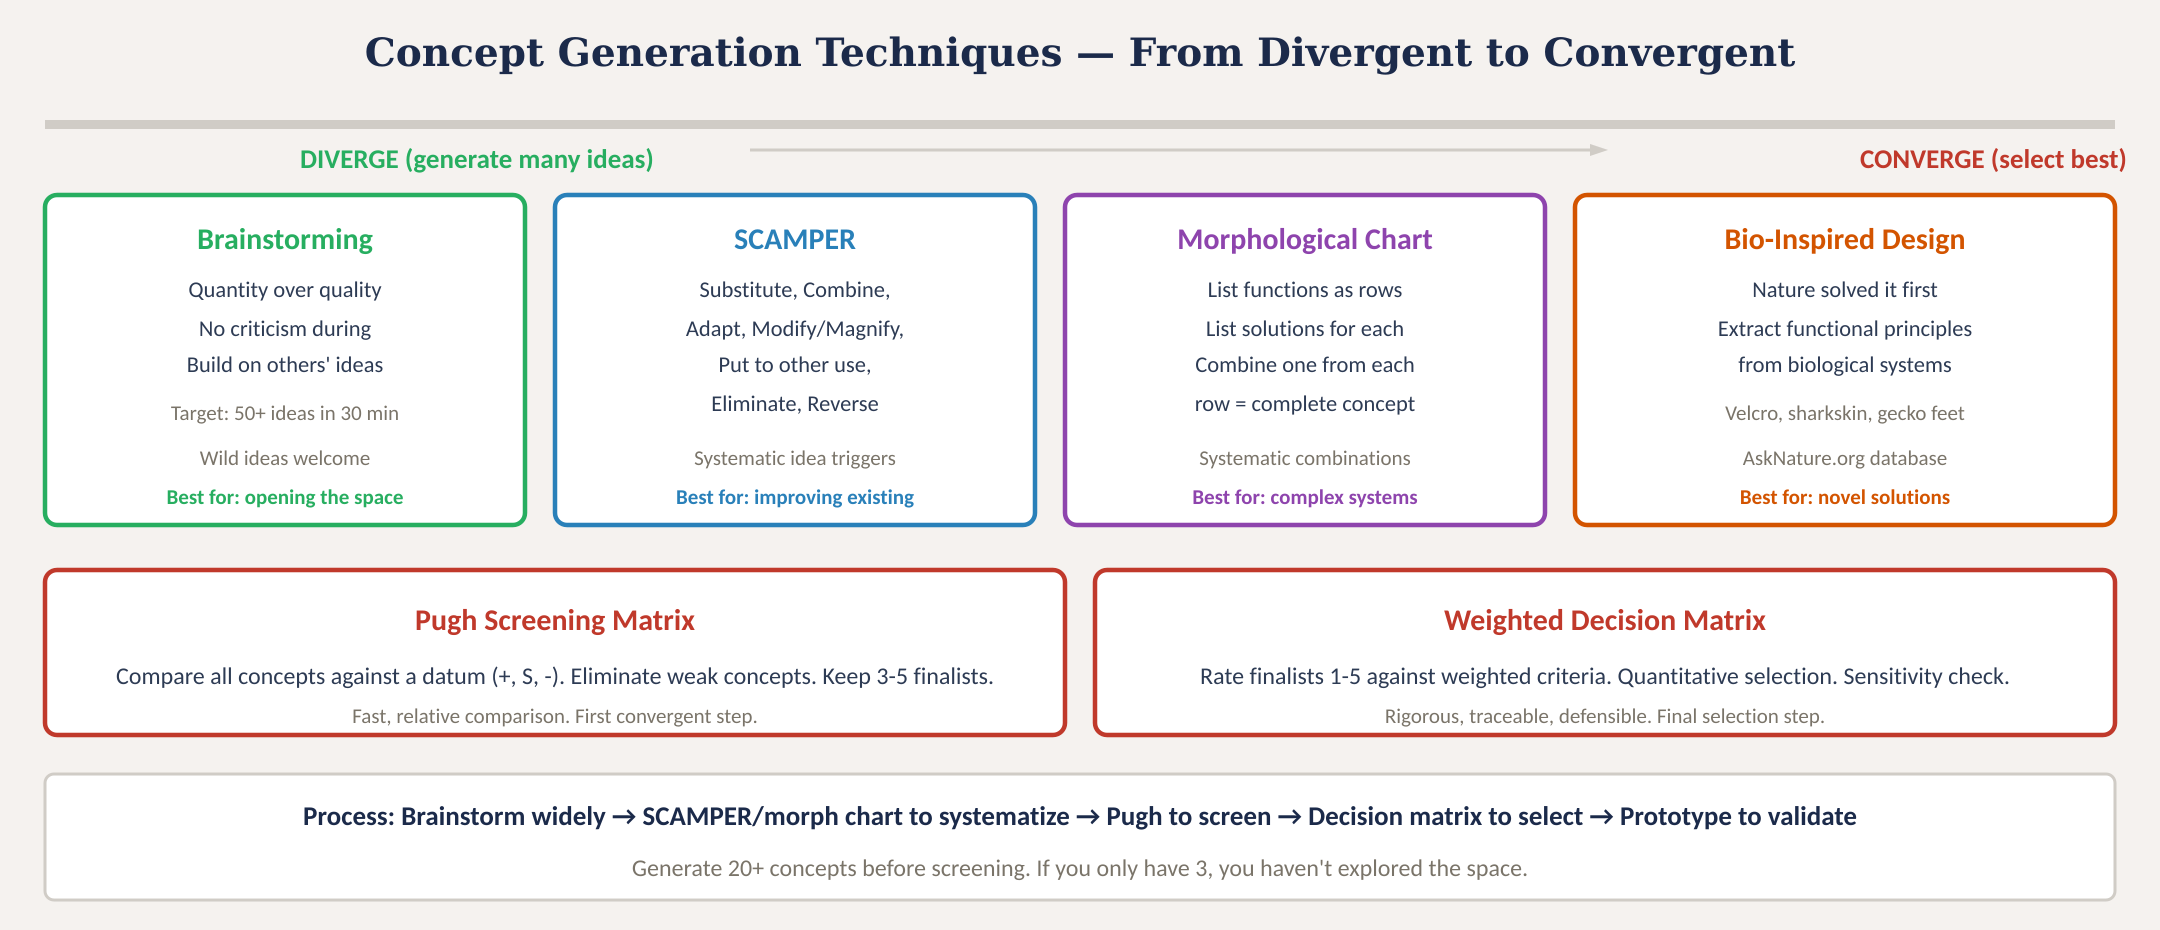
\includegraphics[width=\textwidth]{Concept Generation/fig_generation_techniques.png}
\caption{Concept generation techniques --- divergent to convergent.}\end{figure}

\begin{figure}[ht!]\centering
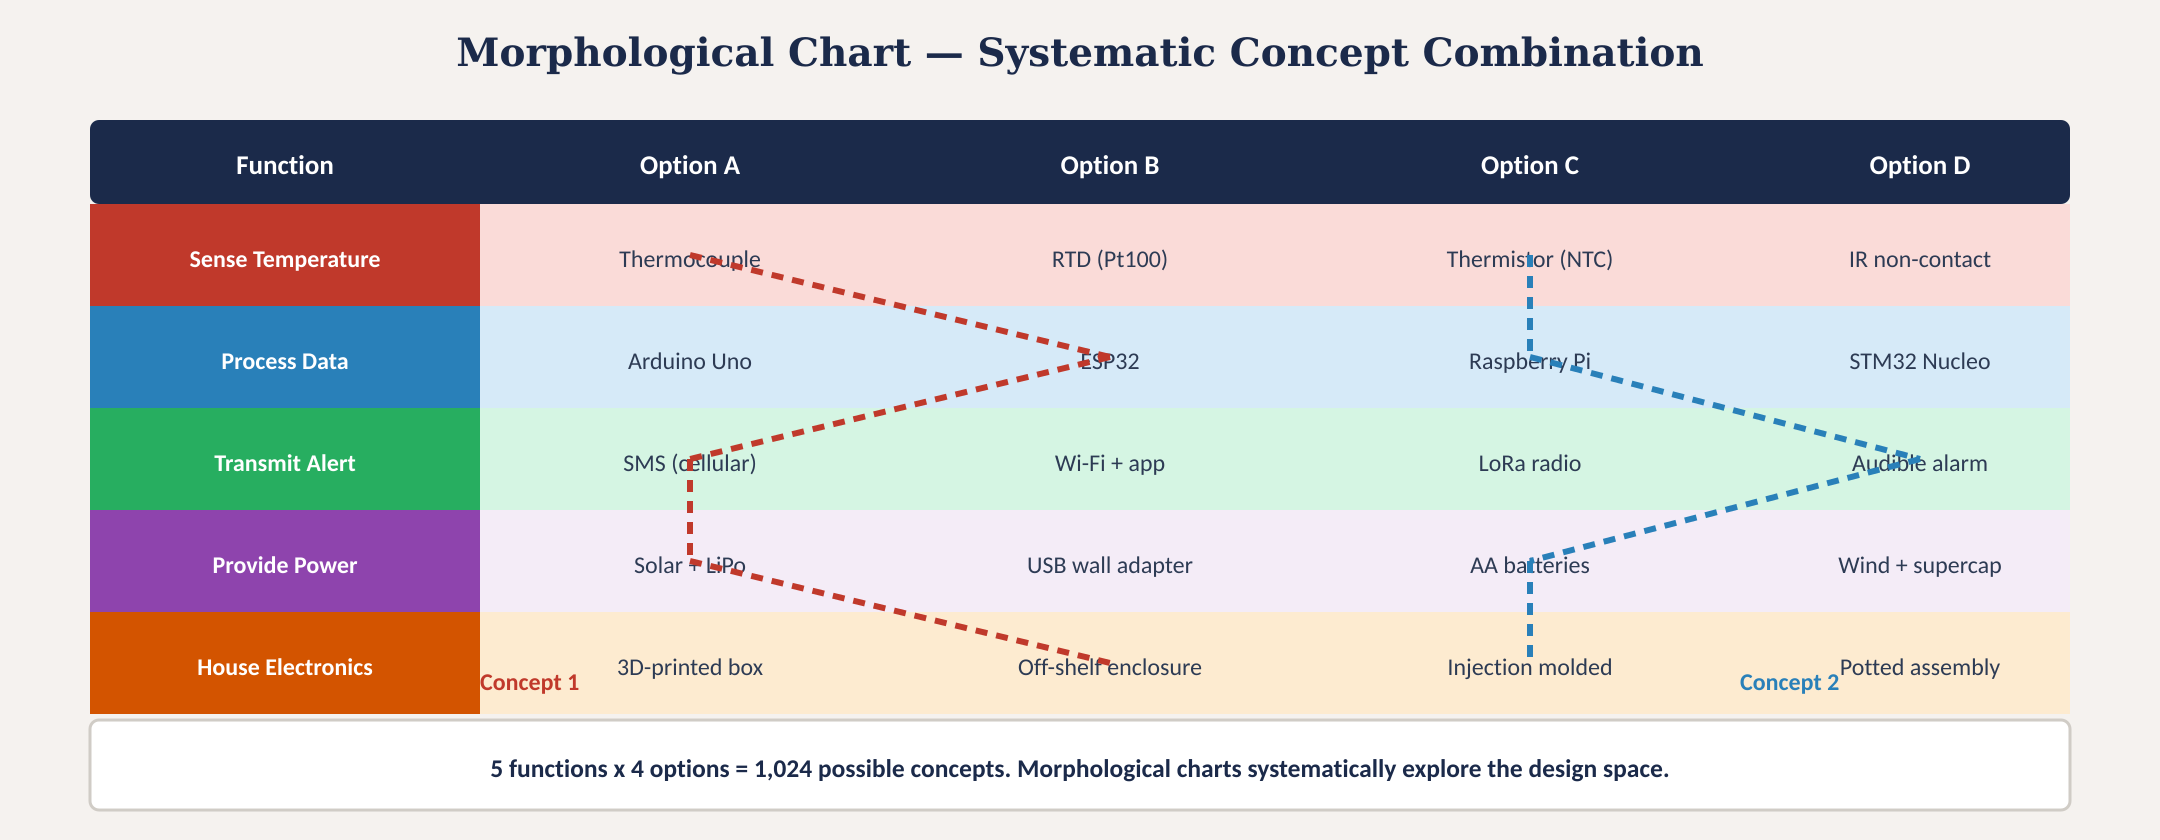
\includegraphics[width=\textwidth]{Concept Generation/fig_morphological_chart.png}
\caption{Morphological chart with systematic concept combinations.}\end{figure}

\begin{figure}[ht!]\centering
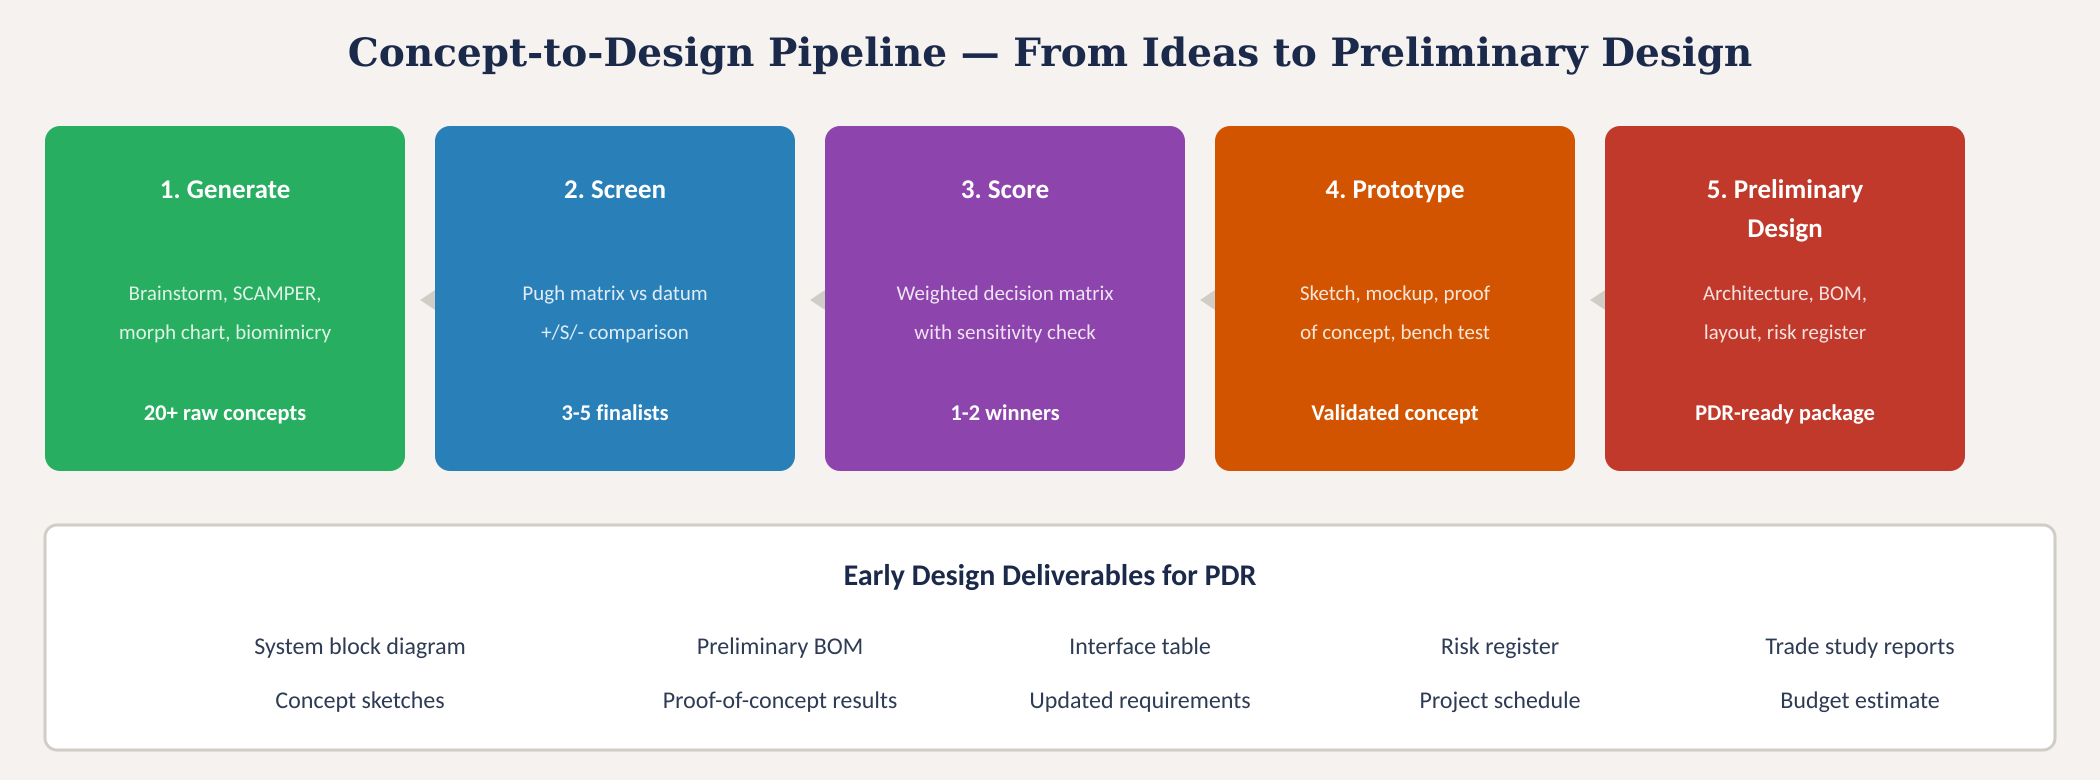
\includegraphics[width=\textwidth]{Concept Generation/fig_concept_pipeline.png}
\caption{Concept-to-design pipeline with PDR deliverables.}\end{figure}

\begin{figure}[ht!]\centering
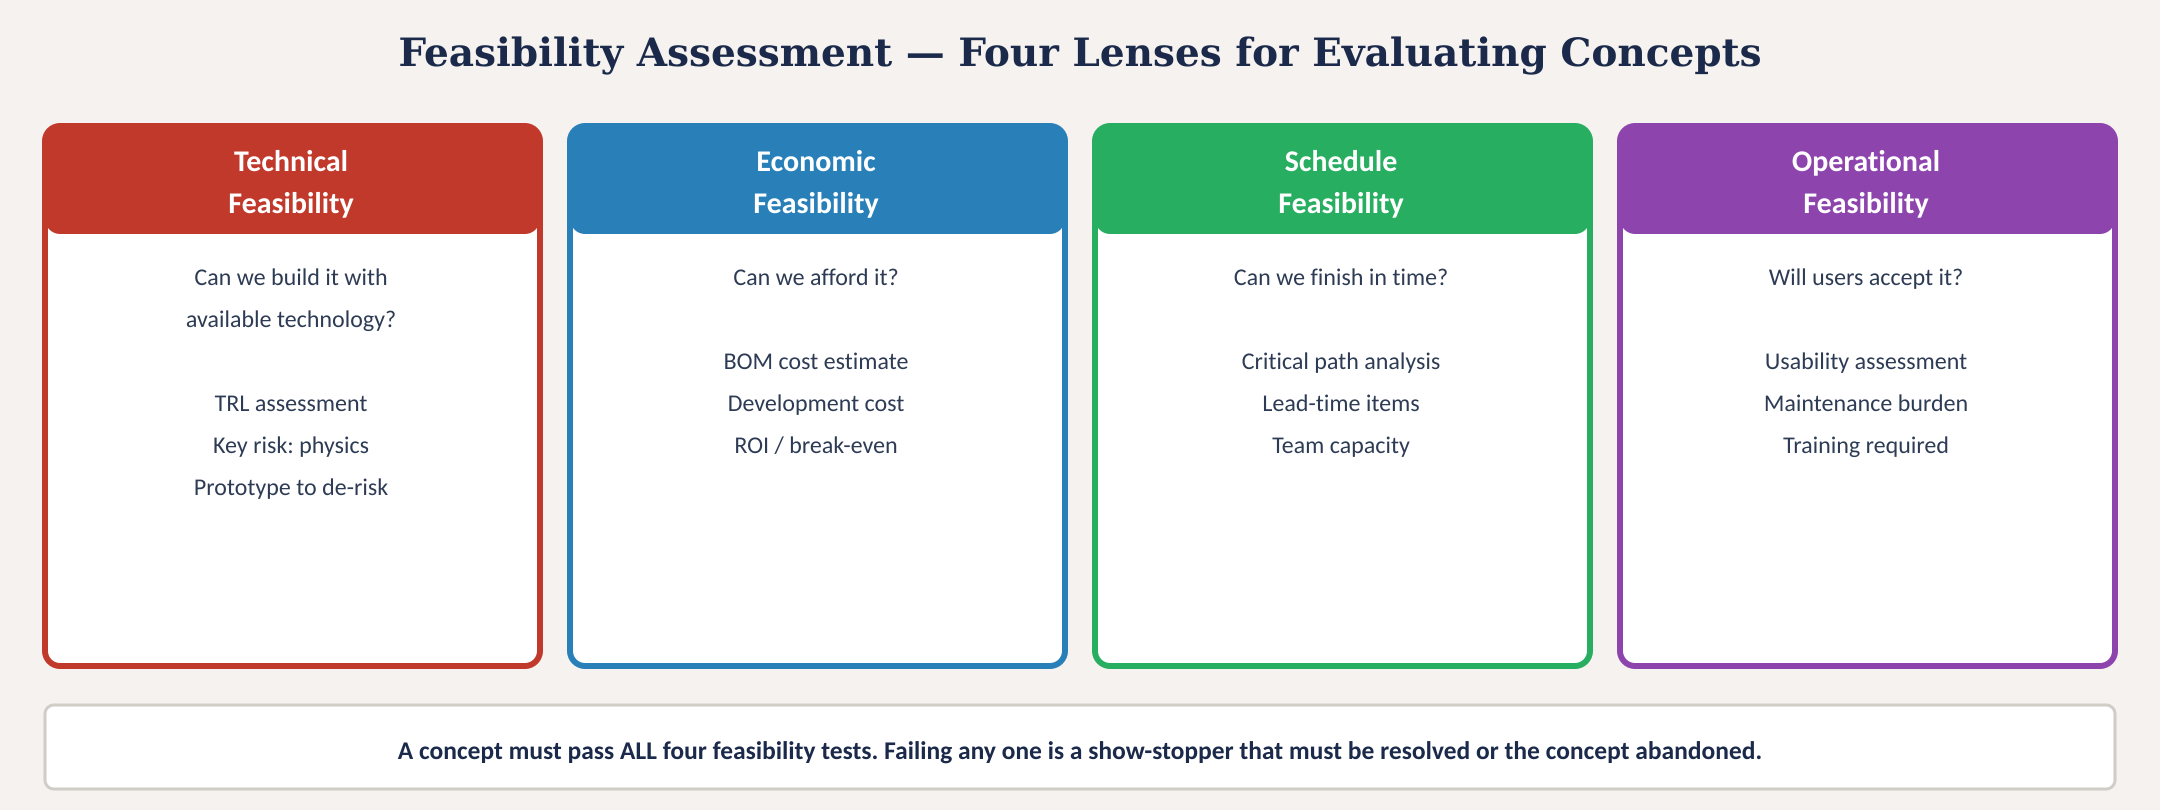
\includegraphics[width=\textwidth]{Concept Generation/fig_feasibility_assessment.png}
\caption{Four-lens feasibility assessment.}\end{figure}

\FloatBarrier
\section{Generating Concepts}
\subsection{The Process: Diverge Then Converge}
The concept generation process has two distinct phases that must be kept separate. \textbf{Divergent} thinking generates as many ideas as possible without evaluation---brainstorming, SCAMPER, morphological charts, and bio-inspired design all belong here. \textbf{Convergent} thinking systematically evaluates and selects---Pugh screening matrices, weighted decision matrices, and feasibility assessments. Generate at least 20 concepts before screening any of them.

Mixing these phases---evaluating ideas during brainstorming---is the single most common failure in concept generation. It kills creativity, biases the team toward incremental solutions, and drastically narrows the design space before it has been explored.

The following process ties this chapter explicitly to the prior ones:
\begin{enumerate}[leftmargin=1.5em]
\item Start from the \textbf{functional decomposition} (Chapter~2). The functions are your rows.
\item Build a \textbf{morphological chart} using those functions: brainstorm 3--5 physical implementation options for each function.
\item Generate \textbf{candidate concepts} by selecting one option from each row. A $5 \times 4$ chart produces 1,024 combinations.
\item \textbf{Screen} via Pugh matrix to eliminate clearly inferior concepts.
\item Build a \textbf{weighted decision matrix} with criteria derived directly from requirements (Chapter~2).
\item Assess \textbf{feasibility and risk} for the top candidates.
\item Feed feasibility results back into requirements and architecture if constraints are discovered.
\end{enumerate}

\subsection{Brainstorming Rules}
Effective brainstorming requires deliberate facilitation. Five rules: (1)~Defer judgment---no criticism, no ``yes, but,'' during ideation. (2)~Go for quantity---target 50+ ideas in 30 minutes; quantity breeds quality. (3)~Build on others' ideas---``yes, and\ldots'' is the only acceptable response. (4)~Encourage wild ideas---they contain seeds of insight that conservative thinking misses. (5)~Sketch, don't just talk---visual communication engages different cognitive pathways and communicates spatial ideas that words cannot.

If your team generated fewer than 15 concepts, something went wrong: the facilitator allowed criticism too early, the problem was framed too narrowly, or the team defaulted to ``the obvious answer'' without exploring alternatives.

\subsection{SCAMPER}
Seven systematic triggers for generating variations from existing concepts or competitor products: \textbf{S}ubstitute (different materials, components, processes), \textbf{C}ombine (merge functions, integrate subsystems), \textbf{A}dapt (borrow from another domain or industry), \textbf{M}odify/Magnify/Minimize (change scale, shape, or proportion), \textbf{P}ut to other use (repurpose for a different function), \textbf{E}liminate (remove components, simplify), \textbf{R}everse/Rearrange (invert flow, change sequence). Apply each trigger to your baseline concept and document every variation, even the ones that seem impractical.

\subsection{Morphological Charts}
The morphological chart is the most powerful systematic tool for concept generation because it directly connects to the functional decomposition from Chapter~2. List the functions from your decomposition as rows. For each function, brainstorm 3--5 physical implementation options as columns. A complete concept is formed by selecting one option from each row.

\needspace{4\baselineskip}
\begin{keyconceptbox}[GreenShield: Morphological Chart]
Using the functional decomposition from Chapter~2:

\begin{center}
\small
\begin{tabularx}{\textwidth}{l X X X}
\toprule
\textbf{Function} & \textbf{Option A} & \textbf{Option B} & \textbf{Option C} \\
\midrule
Sense Temperature & NTC thermistor & DS18B20 digital & Thermocouple + amp \\
Process \& Decide & Arduino Uno & ESP32 & Raspberry Pi Zero \\
Actuate Heater & Mechanical relay & Solid-state relay & Contactor \\
Communicate & GSM/SMS module & Wi-Fi + cloud & LoRa radio \\
Provide Power & Wall adapter 12V & PoE & Solar + battery \\
Operator Interface & 2-line LCD + buttons & OLED + encoder & Web dashboard \\
\bottomrule
\end{tabularx}
\end{center}

This $6 \times 3$ chart produces $3^6 = 729$ possible concept combinations. Three representative concepts:

\textbf{Concept~1} (Low-cost wired): NTC + Arduino + mech.\ relay + GSM + wall adapter + LCD. Estimated cost: \$45.

\textbf{Concept~2} (IoT-connected): DS18B20 + ESP32 + SSR + Wi-Fi + wall adapter + web dashboard. Estimated cost: \$55.

\textbf{Concept~3} (Off-grid autonomous): Thermocouple + ESP32 + contactor + LoRa + solar + OLED. Estimated cost: \$120.

Each concept represents a fundamentally different system architecture---the morphological chart ensures the team explores the design space rather than fixating on the first idea.
\end{keyconceptbox}

\subsection{Bio-Inspired Design}
Extract functional principles from biological systems. Velcro from burdock burrs. Sharkskin riblets for drag reduction. Gecko feet for dry adhesion. Use AskNature.org to search by function. TRIZ (Theory of Inventive Problem Solving) provides 40 inventive principles for resolving design contradictions---situations where improving one parameter degrades another.

\FloatBarrier
\section{Trade Studies and Concept Selection}

Trade studies are the formal, traceable mechanism by which engineering teams select among competing concepts. They belong here---after concepts have been generated---because you cannot evaluate options that do not yet exist. The criteria for evaluation come directly from the requirements (Chapter~2), ensuring that the selection is driven by stakeholder needs rather than team preference.

\subsection{Stage 1: Pugh Screening Matrix}
The Pugh matrix is a fast, qualitative screening tool for eliminating clearly inferior concepts. Select one concept as the \textbf{datum} (reference). Rate every other concept against the datum on each criterion as better ($+$), same (S), or worse ($-$). Count the $+$ and $-$ tallies. Concepts with many more minuses than pluses are eliminated. The Pugh matrix does \emph{not} use weights and does \emph{not} produce a ``winner''---it narrows the field to 2--3 finalists for rigorous quantitative evaluation.

\subsection{Stage 2: Weighted Decision Matrix}
The weighted decision matrix is the primary tool for traceable concept selection. The process:

\begin{enumerate}[leftmargin=1.5em]
\item \textbf{Define criteria} derived from requirements. Typical categories: performance, cost, reliability, manufacturability, power consumption, size/weight, maintainability, schedule risk. Every criterion must trace to at least one requirement.
\item \textbf{Assign weights} that sum to 1.0. Weights reflect the relative importance of each criterion as determined by the requirements priorities (MoSCoW from Chapter~1). Document the rationale for every weight.
\item \textbf{Rate each option} against each criterion on a consistent scale (e.g., 1--5, where 5 is best). Use \emph{data}, not opinion: datasheets, vendor quotes, simulation results, prototype measurements. If you must estimate, document your assumptions.
\item \textbf{Score}: weighted score = $\sum_i w_i \times r_i$. The highest total score is the recommended selection.
\item \textbf{Sensitivity analysis}: vary each weight by $\pm 0.05$ and check if the winner changes. If a small weight change flips the result, the decision is not robust---investigate the discriminating criteria more deeply. A margin of $< 5\%$ between the top two options demands additional data or a prototype comparison.
\item \textbf{Document everything}: the complete matrix, all data sources, weight rationale, sensitivity results, and any dissenting opinions from team members.
\end{enumerate}

\begin{figure}[ht!]\centering
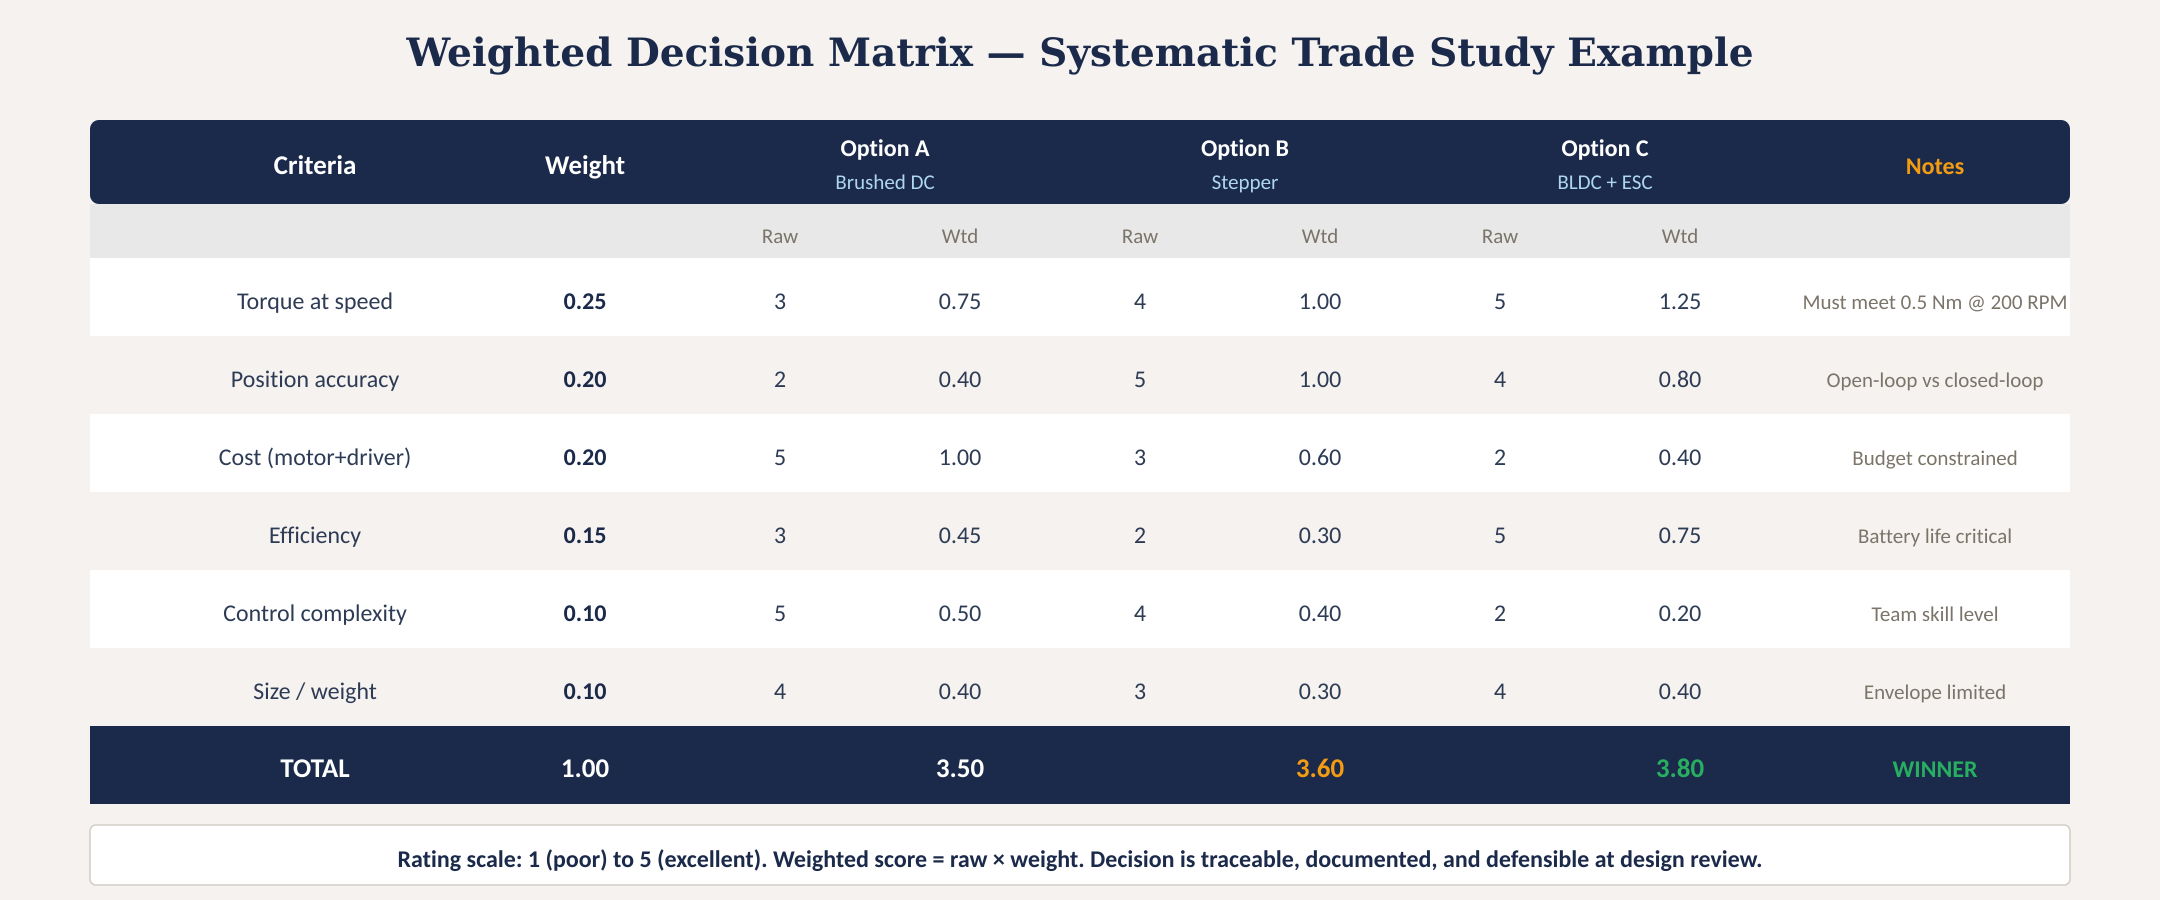
\includegraphics[width=\textwidth]{Requirements and Architecture/fig_decision_matrix.png}
\caption{Weighted decision matrix example: motor selection with six criteria, three options.}\label{fig:matrix}
\end{figure}

\needspace{4\baselineskip}
\begin{warningbox}[Common Trade Study Pitfalls]
\textbf{Straw-man alternatives}: Including clearly inferior options to make the preferred choice ``win.'' Every candidate must be a legitimate contender. \textbf{Anchoring on a favorite}: Rating a preferred option generously and competitors harshly. Assign ratings independently before discussion. \textbf{Criteria not from requirements}: If a criterion does not trace to a requirement, it should not be in the matrix. \textbf{Post-hoc weight adjustment}: Changing weights to produce a desired outcome. Lock weights before scoring.
\end{warningbox}

\FloatBarrier
\section{Risk Assessment}

Risk management begins during concept selection, not after the design is complete. A risk is any event or condition that could prevent the system from meeting its requirements. Every concept carries risks---the question is which risks are acceptable and which require mitigation before committing to a design.

\subsection{The Risk Matrix}
Risks are characterized by two dimensions: \textbf{likelihood} (how probable is the event?) and \textbf{consequence} (how severe is the impact if it occurs?). Both are rated on a 1--5 scale:

\begin{center}
\small
\begin{tabular}{l l l}
\toprule
\textbf{Score} & \textbf{Likelihood} & \textbf{Consequence} \\
\midrule
1 & Remote ($<5\%$) & Negligible (minor rework) \\
2 & Unlikely (5--20\%) & Minor (schedule slip $<1$ week) \\
3 & Possible (20--50\%) & Moderate (redesign of one subsystem) \\
4 & Likely (50--80\%) & Major (cannot meet a key requirement) \\
5 & Near certain ($>80\%$) & Critical (project failure, safety hazard) \\
\bottomrule
\end{tabular}
\end{center}

The \textbf{Risk Priority Number (RPN)} = Likelihood $\times$ Consequence, ranging from 1 to 25. Risks with RPN $\geq 12$ (the ``red zone'') require active mitigation plans before the concept can proceed. Risks with RPN 6--11 (``yellow zone'') should be monitored and have contingency plans. Risks with RPN $\leq 5$ (``green zone'') are accepted.

\subsection{Risk Mitigation Strategies}
Four standard strategies: \textbf{Avoid} (change the design to eliminate the risk---choose a different component, architecture, or approach), \textbf{Mitigate} (reduce likelihood or consequence through redundancy, testing, or design margins), \textbf{Transfer} (shift the risk to another party---insurance, warranties, contractual terms), \textbf{Accept} (acknowledge the risk and proceed---appropriate only for low-RPN items with documented rationale).

\needspace{4\baselineskip}
\begin{keyconceptbox}[GreenShield: Risk Assessment for Concept 3 (Off-Grid)]
\begin{center}
\small
\begin{tabularx}{\textwidth}{X c c c l}
\toprule
\textbf{Risk} & \textbf{L} & \textbf{C} & \textbf{RPN} & \textbf{Mitigation} \\
\midrule
Solar panel insufficient in winter & 4 & 4 & 16 & Add battery sizing margin; test in Dec \\
LoRa range blocked by terrain & 3 & 3 & 9 & Site survey; add repeater option \\
Contactor fails in closed position & 2 & 5 & 10 & Add thermal fuse as backup \\
Thermocouple accuracy insufficient & 3 & 3 & 9 & Calibrate in situ; budget for RTD upgrade \\
\bottomrule
\end{tabularx}
\end{center}

Concept~3's highest risk (RPN~16) is power availability in winter---a showstopper if not mitigated. This risk alone may drive the team toward Concept~1 or~2 (mains-powered) unless the stakeholder requires off-grid capability. Risk analysis directly informs concept selection.
\end{keyconceptbox}

\FloatBarrier
\section{Prototyping and Feasibility}
Four prototype types, each serving a different purpose in the concept development process: \textbf{Proof of Concept (PoC)} tests whether the fundamental physics or algorithm works---does the sensor achieve the required accuracy? Does the control loop stabilize? \textbf{Form/Fit} prototypes test whether the physical design fits the available space and interfaces correctly with adjacent systems. \textbf{Looks-Like/Works-Like} prototypes combine form and function to validate the complete user experience. \textbf{Minimum Viable Product (MVP)} is the simplest version the stakeholder can evaluate for validation.

Build the PoC for the \textbf{highest-risk element FIRST}. This is the single most important scheduling decision in concept development. If the highest-risk element fails, you want to discover that failure as early as possible, when the cost of changing course is lowest.

\subsection{Feasibility Assessment}
Every concept must pass four tests before it can proceed to detailed design. Failing any one is a show-stopper:

\textbf{Technical feasibility}: Can we build it with known technology and available skills? Are the performance requirements achievable with the selected components? What is the technical maturity level?

\textbf{Economic feasibility}: Can we afford it within the project budget? What is the total lifecycle cost (not just the prototype cost)? Does the cost-benefit analysis justify the investment?

\textbf{Schedule feasibility}: Can we finish within the project timeline? Are long-lead-time components identified? Is there schedule margin for iteration?

\textbf{Operational feasibility}: Will the stakeholders accept it? Can the intended users operate and maintain it? Does it comply with all regulatory requirements?

\FloatBarrier
\section{Failure Modes and Effects Analysis (FMEA)}
FMEA is introduced here---during concept selection and early design---because it is most valuable \emph{before} you commit to a design. In MEGN~301, you submit your FMEA at PDR (Sprint~2), alongside your trade study. This timing is intentional: FMEA results should influence your design decisions, not merely document them after the fact.

The FMEA systematically asks: ``What can go wrong?'' For each component, function, or interface in your proposed design, you identify potential failure modes, assess their effects on the system and the user, and take action to reduce risk before building the prototype. See Chapter~6 for the complete FMECA methodology with the RPN calculation ($\text{RPN} = S \times O \times D$). Here, we focus on how to conduct an effective FMEA during the design phase.

\subsection{Conducting a Design-Phase FMEA}
\begin{enumerate}[leftmargin=1.5em]
\item \textbf{List all subsystems and components} from your architecture block diagram (Chapter~2).
\item For each component, ask: \textbf{How can it fail?} Consider electrical failures (open, short, drift), mechanical failures (fracture, wear, loosening), software failures (crash, wrong output, timing), and interface failures (miscommunication, incompatibility).
\item For each failure mode, determine the \textbf{effect} on the system and on the user. Does the system stop working? Does it produce a wrong output? Does it create a safety hazard?
\item \textbf{Rate Severity, Occurrence, and Detection} on 1--10 scales (see Chapter~6 for detailed scales).
\item \textbf{Calculate RPN} and rank failure modes. Focus design effort on the highest-RPN items first.
\item \textbf{Define corrective actions} for high-RPN items: design changes, added redundancy, improved detection, or revised test plans. Document the expected post-action RPN.
\end{enumerate}

\needspace{4\baselineskip}
\begin{warningbox}[FMEA as an Active Design Tool]
In industry, the best engineering teams use the FMEA as an active design tool that drives decisions \emph{before} hardware is built. Your goal is to reach that level of practice: write your FMEA during concept selection and preliminary design, when you still have the freedom to change the architecture, add redundancy, select different components, or redesign interfaces. A well-executed FMEA should result in at least 2--3 concrete design changes. If your FMEA did not change anything about your design, it was not used as a tool---it was used as paperwork.
\end{warningbox}

\needspace{4\baselineskip}
\begin{tipbox}[Safety Hazard Identification]
Pay special attention to failure modes with high severity regardless of RPN. A failure mode with $S = 9$ (safety hazard) and $O = 1$ (very unlikely) still has RPN = 9---which is low. But the consequence of that rare failure could be a fire, an injury, or equipment damage. Industry practice is to flag any failure mode with $S \geq 8$ for mandatory mitigation, regardless of the overall RPN. In MEGN~301, your instructor expects you to identify and address safety hazards in your FMEA and discuss them in your final report.
\end{tipbox}

\FloatBarrier
\section{Design Documentation}
The transition from CDR to the build phase requires a complete documentation package that enables fabrication, procurement, and assembly. Missing or ambiguous documentation is one of the most common causes of schedule delays in student projects.

\subsection{Bill of Materials (BOM)}
The BOM is a complete, structured list of every component needed to build one unit of the system. A minimum BOM for MEGN~301 includes:

\begin{center}
\small
\begin{tabularx}{\textwidth}{l l l l X l l}
\toprule
\textbf{Item} & \textbf{Part \#} & \textbf{Vendor} & \textbf{Qty} & \textbf{Description} & \textbf{Unit Cost} & \textbf{Total} \\
\midrule
1 & DS18B20 & DigiKey & 2 & Digital temp sensor, TO-92 & \$3.50 & \$7.00 \\
2 & --- & Custom & 1 & Sensor bracket, PLA 3D print & \$1.20 & \$1.20 \\
\bottomrule
\end{tabularx}
\end{center}

Include \emph{everything}: electronic components, fasteners, wire, solder, 3D-printed parts (with estimated material cost), and any consumables. The BOM is a living document that is updated whenever the design changes. At FDR, the BOM should reflect exactly what is in the delivered prototype.

\needspace{4\baselineskip}
\begin{tipbox}[Plan B Components]
For every critical or sole-source component in your BOM, identify an alternative (``Plan B'') and record its part number and vendor in a notes column. If your specialty MOSFET, water pump, or sensor goes out of stock the week before your CDR deadline, you need to order the backup \emph{immediately}---not start a new search. This is especially important for the \textit{Sous Vide Supreme} (specialty heating elements) and \textit{Sol-Mate Purification Pal} (solar charge controllers) projects, where lead times can exceed two weeks.
\end{tipbox}

\needspace{4\baselineskip}
\begin{tipbox}[Free Electronics Supplies]
Bulk wire (18~\&~24~AWG in multiple colors), heat shrink tubing, and solderable perf boards are available \textbf{for free in BBW160} from the TAs during normal office hours (see Appendix~B of the Project Document for the complete list and per-foot pricing for budget tracking). Do not waste your project budget on items the department provides. When calculating your final BOM cost, include the per-foot wire pricing from Appendix~B (\$0.19/ft for 18~AWG, \$0.08/ft for 24~AWG) so your accounting is complete.
\end{tipbox}

\needspace{4\baselineskip}
\begin{warningbox}[The Spring Break Shipping Trap]
Check the calendar: Spring Break begins March~24. Campus shipping and receiving, the machine shop, and all lab facilities are \textbf{closed} that week. If a component fails during your Sprint~4 Subsystem Demo (March~10--12) and you need a replacement for your Complete System Demo (Sprint~5), you must order it \emph{immediately}---not after break. Plan your procurement so that all critical components arrive before March~21. The same logic applies to 3D prints and machined parts: submit them early enough to allow for iteration \emph{before} the campus shuts down.
\end{warningbox}

\needspace{4\baselineskip}
\begin{warningbox}[Short Weeks in Sprint 2 and 3]
Two disrupted weeks fall early in the semester: \textbf{Career Day (February~3, no Tuesday class)} lands in the middle of Sprint~2 (PDR), and \textbf{Presidents' Day Break (February~17, no Tuesday class)} falls as you transition into the manufacturing phase of Sprint~3 (CDR). Losing an in-person lab day often throws off poorly planned sprints. Look at the course calendar during your first team meeting and build your sprint schedule around these gaps---do not discover them the night before a deliverable is due.
\end{warningbox}

\subsection{Wiring Diagrams and Schematics}
Every electrical connection in your system must be documented in a wiring diagram that shows: (1)~every component with its designator, (2)~every wire with its color, gauge, and length, (3)~every connector with its part number and pinout, and (4)~power distribution including fuses and voltage regulators. The wiring diagram is the electrical equivalent of the ICD---it is the contract that defines how subsystems are physically connected.

\subsection{Software Architecture and Flowcharts}
If your system includes a microcontroller, document the firmware architecture with a programming flowchart showing: main loop structure, interrupt service routines, state machine transitions, sensor reading and processing, actuator control logic, communication protocols, and error handling. The flowchart should be detailed enough that another engineer could implement the firmware from it.

\subsection{CAD Models and Engineering Drawings}
All custom mechanical components must have complete CAD models with associated engineering drawings that include: material specification, critical dimensions with tolerances, surface finish requirements, and manufacturing notes (e.g., ``3D print in PLA, 0.2\,mm layer height, 40\% infill'' or ``machine from 6061-T6 aluminum per attached order of operations''). For injection-molded parts, the drawing must include draft angles, parting line location, and gate location (see the Injection Molding chapter).

\needspace{4\baselineskip}
\begin{tipbox}[DFM at CDR]
All polymer components in your design must be designed to be immediately manufacturable by injection molding, even if your prototype is 3D-printed. This means draft angles on all walls, uniform wall thickness, proper rib and boss proportions, and identified parting lines. The Manufacturing Design Review (Sprint~3) will evaluate your polymer parts against the DFM checklist in the Injection Molding chapter. Consult that checklist \emph{before} finalizing your CAD models.
\end{tipbox}

\needspace{4\baselineskip}
\begin{tipbox}[Strategic Resin Selection (Budget Saver)]
The resin printers on campus support two materials at very different price points: Elegoo ABS-Like resin at \$15/kg and Siraya Tech Blu Nylon-Like resin at \$38/kg (see Appendix~A of the Project Document for print settings). Use the \$15/kg ABS-like resin for basic structural enclosures, brackets, and cosmetic parts. Reserve the \$38/kg Nylon-like resin only for parts that specifically require high toughness, wear resistance, or repeated flexure---such as gears, snap-fit clips, or living hinges. A single strategic resin choice can save \$20--40 of your project budget.
\end{tipbox}

\FloatBarrier
\section{Artifact Handoff: What Chapter~3 Produces}

\begin{center}
\small
\begin{tabularx}{\textwidth}{l X X}
\toprule
\textbf{Artifact from Ch.~3} & \textbf{Primary Contents} & \textbf{Used Directly In\ldots} \\
\midrule
Morphological chart & Functions $\times$ implementation options & Documents design space explored \\
Pugh screening matrix & Qualitative $+$/S/$-$ ratings vs.\ datum & Justifies elimination of weak concepts \\
Weighted decision matrix & Quantitative scores, weights, sensitivity & Traceable rationale for selected concept \\
Risk register & Risks, RPNs, mitigation plans & Informs test priority (Ch.~4), design margins \\
Feasibility assessment & Technical/economic/schedule/operational & Supports PDR-to-CDR transition \\
Selected concept description & Architecture, BOM, preliminary layout & Basis for detailed design, test planning (Ch.~4) \\
Reverse engineering analysis & Component inventory, interface inventory, constraints & Informs ICDs (Ch.~2), concept generation, FMEA \\
FMEA & Failure modes, RPNs, corrective actions & Drives design changes before build; safety discussion in final report \\
Design documentation & BOM, wiring diagrams, flowcharts, CAD & Enables fabrication, procurement, and assembly at CDR \\
\bottomrule
\end{tabularx}
\end{center}

\needspace{4\baselineskip}
\begin{tipbox}[Industry SE Parallels]
This chapter corresponds to INCOSE SEH Section~4.4 (Architecture Definition, continued) and~4.5 (Design Definition). The trade study process aligns with NASA SP-2016-6105 Section~6.8 (Decision Analysis). Risk management follows ISO~31000 principles and maps to INCOSE SEH Section~4.3.7. In industry, the selected concept, trade study reports, and risk register are primary deliverables reviewed at the Preliminary Design Review (PDR). The transition from PDR to CDR is gated on demonstrating that the selected concept is feasible and that high risks have credible mitigation plans.
\end{tipbox}

\FloatBarrier
\section{Practice Questions}
Questions are tiered: \textbf{C} = Comprehension, \textbf{A} = Application, \textbf{CT} = Critical Thinking.
\begin{enumerate}[leftmargin=1.5em]
\item \textbf{[A]} Create a morphological chart for a campus recycling station with at least 4 functions and 3 options each. Trace two complete concept paths and describe how each represents a fundamentally different architecture.
\item Your team brainstormed only 5 concepts in 20 minutes. What went wrong? What facilitation techniques would you use to increase output?
\item Construct a weighted decision matrix comparing three sensor options for a battery-powered outdoor monitoring system. Define at least five criteria with weights derived from requirements. Perform a sensitivity analysis on the highest-weighted criterion.
\item Your proof-of-concept test shows the sensor accuracy is 1.2$^{\circ}$ C against a 0.5$^{\circ}$ C requirement. What are your options? Frame your answer using the requirements-architecture iteration process.
\item A trade study produces scores of 3.82 vs 3.79 between two motor options. What do you do before accepting the winner?
\item Create a $5 \times 5$ risk matrix for an outdoor environmental monitoring system. Identify at least four risks, rate each for likelihood and consequence, calculate RPNs, and propose mitigation strategies for any risk in the red zone (RPN $\geq 12$).
\item Explain why you cannot perform a meaningful trade study before generating concepts. What information do you need from Chapter~2 to construct the evaluation criteria?
\item Your morphological chart has 5 functions with 4 options each, yielding 1,024 possible concepts. You cannot evaluate all of them. Describe a systematic process for narrowing the field to 3--5 finalists before building a weighted decision matrix.
\end{enumerate}

\subsection{Answers}
\begin{enumerate}[leftmargin=1.5em]
\item Functions: (a) Identify material (vision sensor, weight sensor, user button, barcode scanner), (b) Sort material (rotating drum, conveyor + diverter, robotic arm, gravity chute), (c) Compact material (hydraulic press, screw compressor, none, manual), (d) Store material (single bin, multi-compartment bin, bag dispenser, pneumatic tube). Concept Path 1 (automated): vision + conveyor + hydraulic press + multi-compartment = high-throughput, high-cost industrial architecture. Concept Path 2 (user-assisted): user button + gravity chute + none + bag dispenser = low-cost, low-maintenance, relies on user compliance. These are fundamentally different because Path 1 requires power, processing, and mechanical complexity while Path 2 is passive.

\item Common failures: criticism during ideation (``that won't work''), too-narrow problem framing, jumping to solutions, dominant team member shutting down discussion, or failing to use systematic techniques. Fixes: enforce ``yes, and'' rule, use SCAMPER triggers to force variation, sketch silently for 5 minutes before sharing (brainwriting), assign a facilitator who does not contribute ideas, use the morphological chart to systematically explore the space.

\item Criteria: power consumption (0.30---battery life is paramount), accuracy (0.25---core performance requirement), cost (0.20---budget constraint), operating temperature range (0.15---outdoor exposure), availability/lead time (0.10---schedule). Options: Sensor A (RTD, high accuracy, high power), Sensor B (NTC thermistor, moderate accuracy, low power), Sensor C (digital IC, good accuracy, moderate power). Rate 1--5, compute weighted scores. Sensitivity: vary power consumption weight from 0.25 to 0.35. If the winner changes, the decision is sensitive to how much you value battery life vs.\ accuracy---investigate further or prototype both.

\item Four options, in order of preference: (1) Investigate root cause---is the 1.2\,\degC\ error from the sensor, the signal conditioning, the ADC, or the test setup? Fix the implementation. (2) Select a different sensor with better specifications (trade study with accuracy as a high-weight criterion). (3) Negotiate with the stakeholder to relax the requirement to $\pm 1.5$\,\degC\ if the application can tolerate it (formal change request with documented rationale). (4) Add calibration compensation in firmware to correct systematic bias. Option (3) is a requirements--architecture iteration; it must go through change control.

\item Sensitivity analysis: vary each weight by $\pm$0.05 and check if the winner changes. A 0.03 margin is extremely tight---within noise for subjective ratings. Investigate the criteria where the two options diverge most. If the winner is sensitive to one criterion, get better data for that criterion (datasheet comparison, vendor consultation, prototype test). Consider prototyping both finalists for a direct head-to-head comparison.

\item Example risks for outdoor monitoring: (a) Solar panel degraded by hail: L=2, C=4, RPN=8 (yellow; mitigate with protective cover or accept with spare). (b) Antenna corroded by salt air: L=3, C=3, RPN=9 (yellow; specify marine-grade antenna). (c) Battery capacity insufficient in winter: L=4, C=4, RPN=16 (red; mitigate with larger battery, power management, and winter testing). (d) Enclosure seal failure from UV degradation: L=3, C=5, RPN=15 (red; mitigate with UV-rated gasket material and 2$\times$ solar exposure testing). Both red-zone items require active mitigation with specific design changes and test plans before proceeding.

\item Trade studies require evaluation criteria, which come from requirements (Chapter~2). Without requirements, criteria are arbitrary and the selection is untraceable. You also need candidate concepts to evaluate---you cannot score options that do not exist. The correct sequence is: requirements $\to$ concept generation $\to$ trade study. Reversing this order leads to confirmation bias (writing requirements that favor a preselected solution).

\item (1) Apply engineering judgment to eliminate obviously infeasible combinations (e.g., solar power + high-power-draw actuator in a budget-constrained system). (2) Use Pugh screening with $+$/S/$-$ ratings against a datum concept for the remaining combinations. This is fast and qualitative. (3) Take the top 3--5 survivors from Pugh into a full weighted decision matrix. This staged approach reduces a 1,024-concept space to a manageable evaluation set without losing good candidates.
\end{enumerate}

\FloatBarrier
\chapter{Verification, Validation \& Test Plans}

\vspace{1em}

This chapter covers the right side of the V-Model: the systematic process of confirming that the system you built satisfies both the written requirements (verification) and the stakeholder's actual operational needs (validation). Verification and validation are the mechanisms that close the loop on every artifact produced in Chapters~1--3. Without rigorous V\&V, requirements are aspirational statements rather than enforceable contracts, and the team has no objective evidence that the system works.

\needspace{4\baselineskip}
\begin{keyconceptbox}[Bottom Line]
Verification asks ``did we build it right?'' (test against specs). Validation asks ``did we build the right thing?'' (test against the stakeholder's actual need). Assign a TAID method to every requirement \emph{when you write it}. Maintain a VCRM from day one. Write test procedures that another engineer could reproduce without your help. Report measured values, not just PASS/FAIL.
\end{keyconceptbox}

\vspace{1em}

\FloatBarrier
\section{Verification vs.\ Validation}
\begin{figure}[ht!]\centering
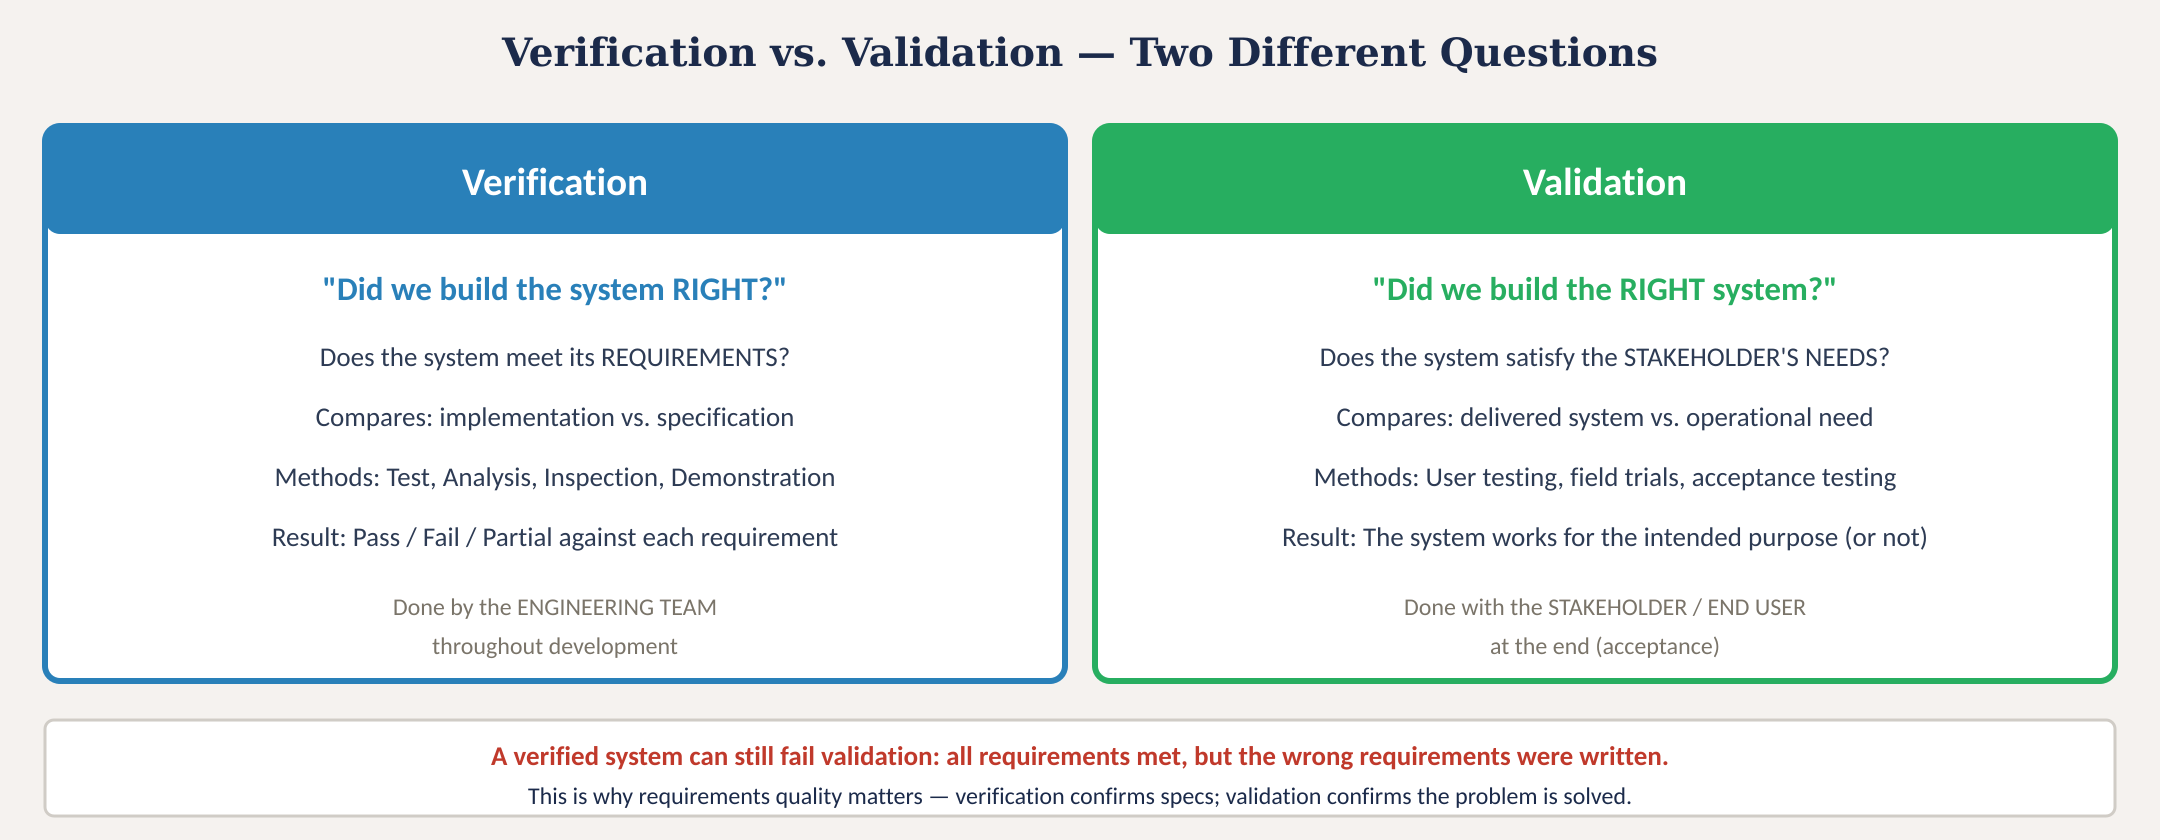
\includegraphics[width=\textwidth]{Verification, Validation, and Test Plans/fig_vv_comparison.png}
\caption{Verification (meets requirements) vs.\ validation (meets needs) --- two different questions.}\label{fig:vv}
\end{figure}

\textbf{Verification} asks: ``Did we build the system RIGHT?'' It compares the implemented system against the written specification. Done by the engineering team using Test, Analysis, Inspection, or Demonstration (TAID). Each requirement receives an individual PASS/FAIL verdict.

\textbf{Validation} asks: ``Did we build the RIGHT system?'' It compares the delivered system against the stakeholder's actual operational need. Done with the stakeholder through user testing, field trials, or acceptance testing.

\needspace{4\baselineskip}
\begin{warningbox}[A Verified System Can Fail Validation]
All requirements met perfectly, but the wrong requirements were written. This is why requirements quality matters --- verification confirms specs; validation confirms the problem is actually solved. You need both.
\end{warningbox}

\FloatBarrier
\section{Four Verification Methods --- TAID}
\begin{figure}[ht!]\centering
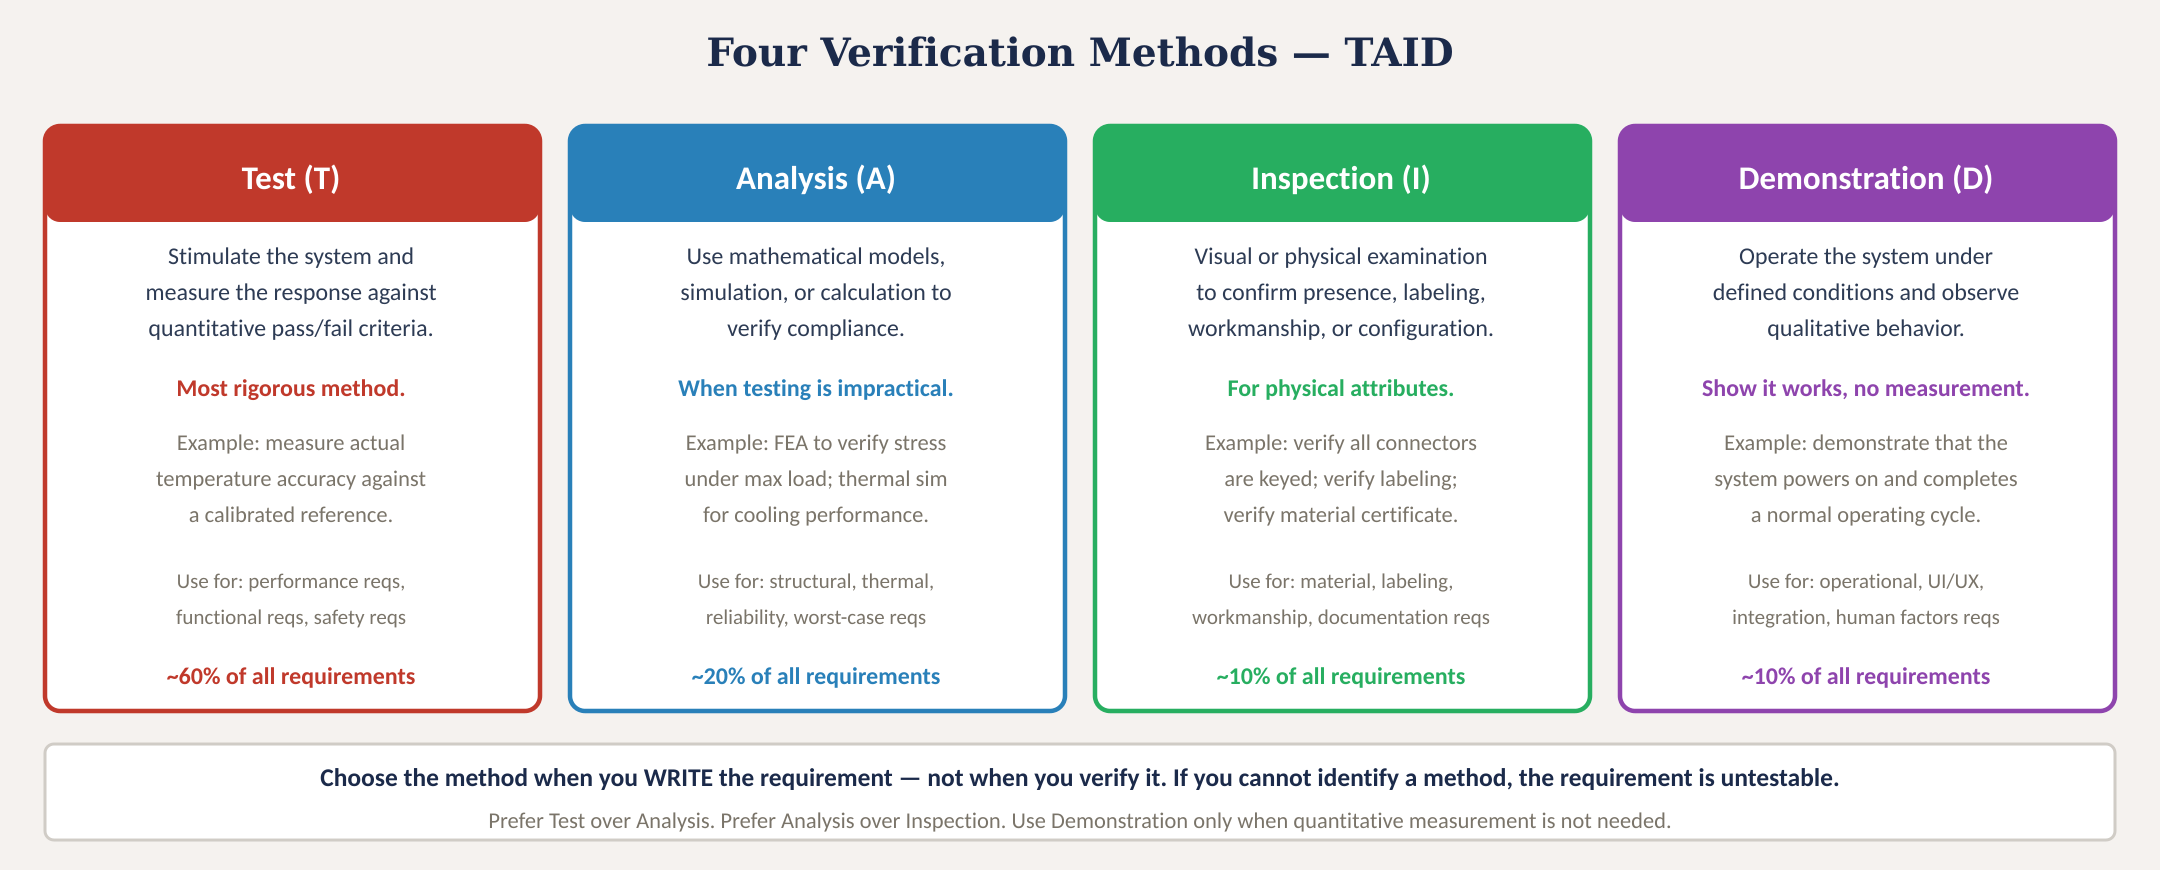
\includegraphics[width=\textwidth]{Verification, Validation, and Test Plans/fig_taid_methods.png}
\caption{Test, Analysis, Inspection, and Demonstration with usage percentages and selection guidance.}\label{fig:taid}
\end{figure}

\begin{itemize}[leftmargin=1.5em]
\item \textbf{Test (T, $\sim$60\% of reqs)}: Stimulate the system and measure the response against quantitative criteria. Most rigorous. Preferred whenever feasible.
\item \textbf{Analysis (A, $\sim$20\%)}: Mathematical models, simulation, or calculation. Used when testing is impractical (FEA, thermal sim, worst-case analysis). Must document assumptions.
\item \textbf{Inspection (I, $\sim$10\%)}: Visual/physical examination --- presence, labeling, workmanship, material certificates.
\item \textbf{Demonstration (D, $\sim$10\%)}: Operate under defined conditions and observe qualitative behavior. No measurement. Used when quantitative testing is not needed.
\end{itemize}

\needspace{4\baselineskip}
\begin{tipbox}[Assign the Method When You Write the Requirement]
If you cannot identify a verification method, the requirement is untestable and must be rewritten. The method check is the single best quality gate for requirements.
\end{tipbox}

\FloatBarrier
\section{Writing Test Plans}
\subsection{What Makes a Good Test Plan}
The gold standard: another engineer with no project knowledge can reproduce your results exactly. Five qualities: \textbf{Traceable} (maps to requirement IDs), \textbf{Reproducible} (specific enough for independent replication), \textbf{Binary} (quantitative pass/fail, no judgment calls), \textbf{Complete} (all sections filled), \textbf{Executed as written} (no ad-hoc deviations).

\subsection{Test Procedure Structure}
\begin{figure}[ht!]\centering
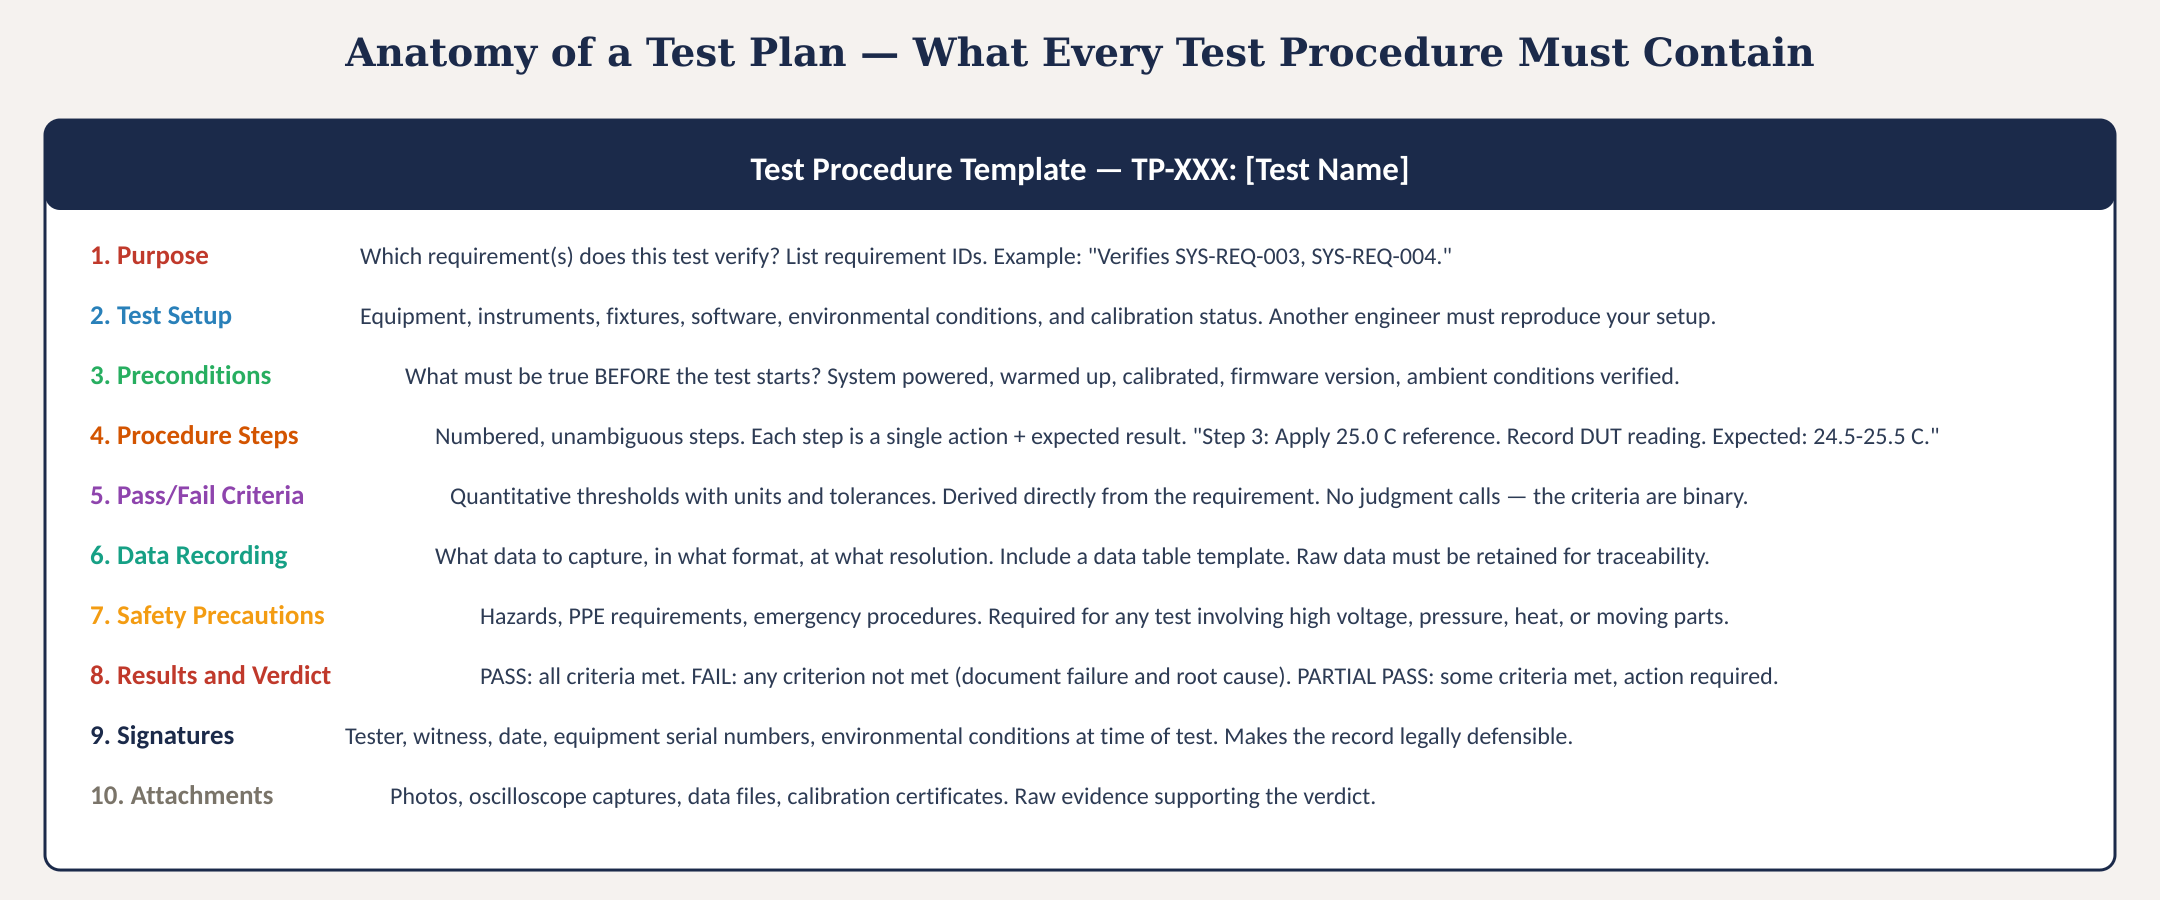
\includegraphics[width=\textwidth]{Verification, Validation, and Test Plans/fig_test_plan_template.png}
\caption{Complete test procedure template with all 10 required sections.}\label{fig:tp}
\end{figure}

Every test procedure contains: (1) Purpose --- requirement IDs verified; (2) Test setup --- equipment with model numbers and calibration; (3) Preconditions --- system state before starting; (4) Procedure steps --- numbered, single-action, imperative voice, with expected results; (5) Pass/fail criteria --- quantitative thresholds from requirements; (6) Data recording --- format, resolution, blank table; (7) Safety precautions; (8) Results and verdict; (9) Signatures; (10) Attachments.

\subsection{Writing Good Procedure Steps}
Each step is a single action with an expected result. Use specific values (``Set reference bath to 25.0 $\pm$ 0.1\,$^{\circ}$ C''), not vague instructions (``check temperature''). Include wait times for stabilization. Imperative voice: ``Set\ldots'' ``Record\ldots'' ``Verify\ldots''

\FloatBarrier
\section{Handling Results}
\begin{figure}[ht!]\centering
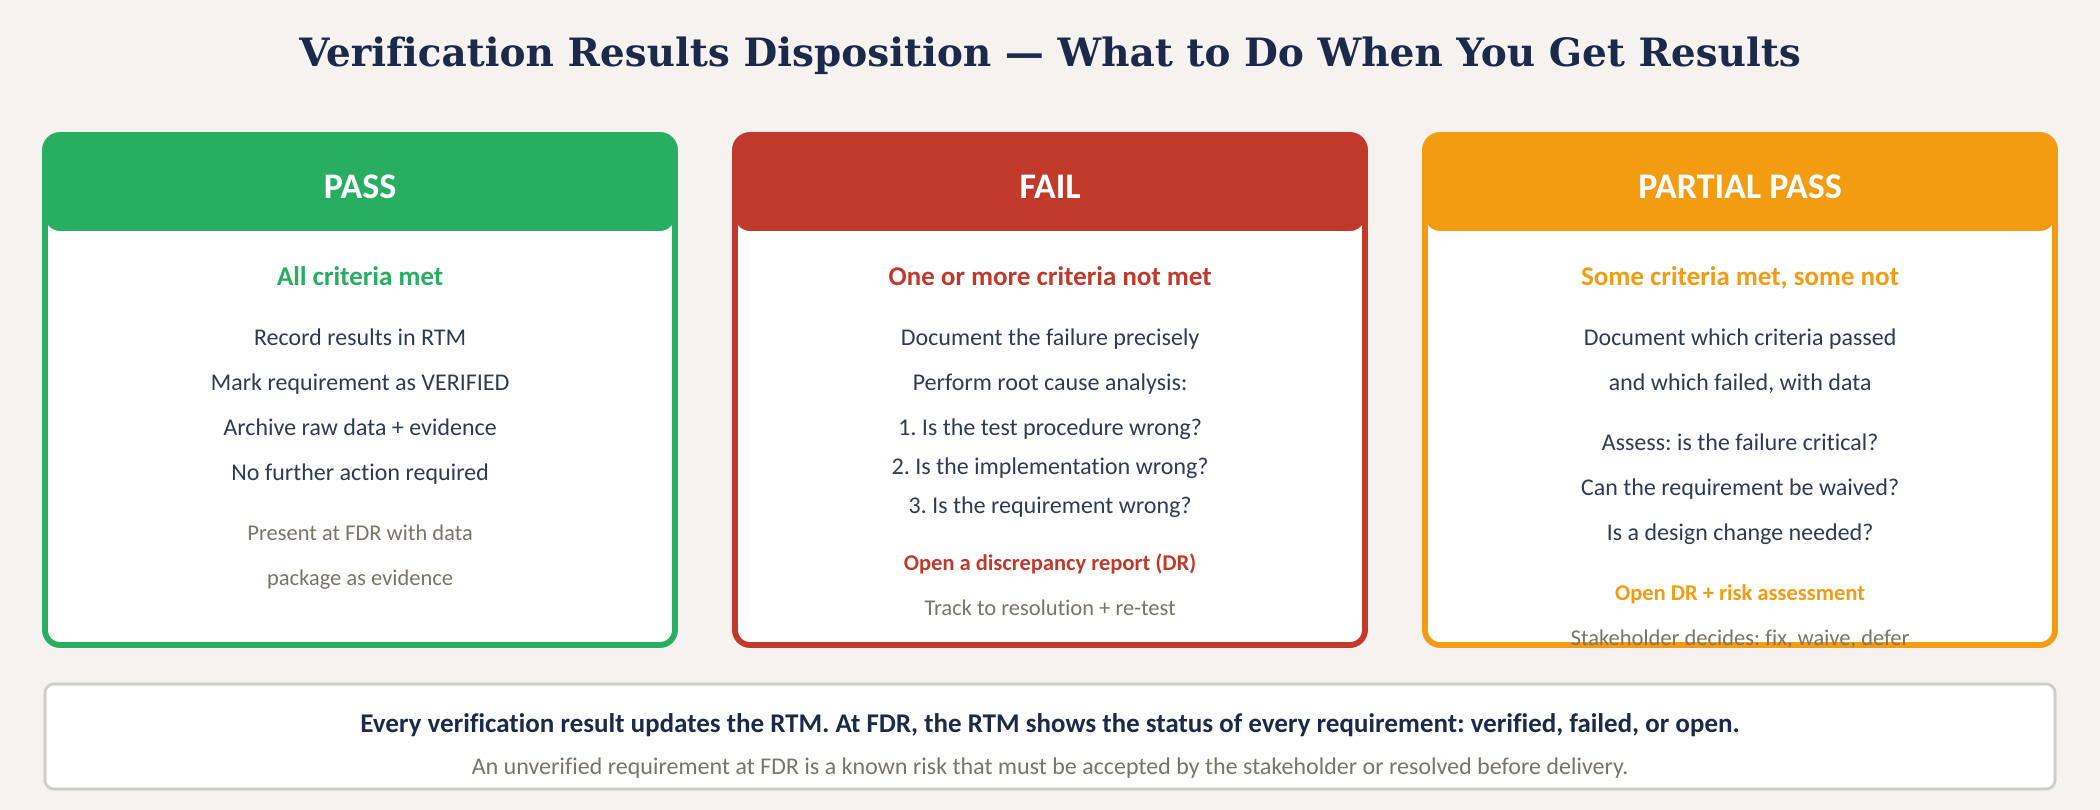
\includegraphics[width=\textwidth]{Verification, Validation, and Test Plans/fig_results_disposition.png}
\caption{Three verification outcomes: PASS, FAIL, PARTIAL PASS with disposition workflows.}\label{fig:disp}
\end{figure}

\subsection{PASS}
All criteria met. Record results in RTM, mark requirement VERIFIED, archive raw data. Include actual measurement values, not just ``PASS.''

\subsection{FAIL}
One or more criteria not met. Root cause analysis in order: (1) Is the test procedure wrong? (2) Is the implementation wrong? (3) Is the requirement wrong? Open a Discrepancy Report (DR), assign corrective action, track to resolution, re-test after correction.

\subsection{PARTIAL PASS}
Some criteria met, some not. Document which passed and which failed with data. Three resolution paths: \textbf{Fix} (redesign + re-test), \textbf{Waive} (stakeholder formally accepts the deviation with documented risk), or \textbf{Defer} (postpone with a plan and deadline). A waiver transfers risk to the stakeholder.

\subsection{Root Cause Analysis}
Three possible root causes, investigated in order: (1) the test is wrong (procedure error, calibration issue); (2) the implementation is wrong (most common); (3) the requirement is wrong (overly conservative or based on incorrect assumptions). Changing a requirement requires formal change control --- never silently.

\needspace{4\baselineskip}
\begin{tipbox}[Root Cause as Differential Diagnosis]
Think of root cause analysis like a doctor's differential diagnosis: (1)~Is the \emph{test} sick? Check your procedure, calibration, and equipment before blaming the patient. (2)~Is the \emph{patient} sick? The most common case---your implementation has a defect. (3)~Is our \emph{definition of healthy} wrong? The rarest but most important case---the requirement itself is based on incorrect assumptions. Always investigate in this order. Jumping to ``the requirement must be wrong'' without first verifying your test procedure is the engineering equivalent of malpractice.
\end{tipbox}

\FloatBarrier
\section{The VCRM}
The Verification Cross-Reference Matrix (VCRM) links every requirement to its verification method, test procedure, and current status. It is the single most important tracking artifact in the V\&V process. Maintain the VCRM from the day you write your first requirement. At FDR, the VCRM tells the complete story of what was verified, how, and with what results.

VCRM columns: Req ID, Requirement Text, Type (F/P/NFR), Verification Method (T/A/I/D), Test Procedure ID, Responsible Engineer, Status (Open/In Progress/Verified/Failed/Waived/Deferred), Date Verified, Notes.

\subsection{VCRM Evolution Over Time}
The VCRM is a living document that evolves through the project lifecycle:

\needspace{4\baselineskip}
\begin{keyconceptbox}[GreenShield: VCRM Fragment at Three Milestones]
\textbf{At PDR} (requirements defined, methods assigned):
\begin{center}\small
\begin{tabularx}{\textwidth}{l X l l l}
\toprule
\textbf{ID} & \textbf{Requirement} & \textbf{Method} & \textbf{Test ID} & \textbf{Status} \\
\midrule
SYS-01 & Monitor temp $\geq$1/min & T & --- & Open \\
SYS-02 & Activate heater when $T < T_{\text{set}}$ & T & --- & Open \\
SYS-03 & Activation within 60\,s & T & --- & Open \\
SYS-04 & SMS alert within 120\,s & D & --- & Open \\
\bottomrule
\end{tabularx}
\end{center}

\textbf{At CDR} (test procedures drafted):
\begin{center}\small
\begin{tabularx}{\textwidth}{l X l l l}
\toprule
\textbf{ID} & \textbf{Requirement} & \textbf{Method} & \textbf{Test ID} & \textbf{Status} \\
\midrule
SYS-01 & Monitor temp $\geq$1/min & T & TP-001 & Open \\
SYS-02 & Activate heater when $T < T_{\text{set}}$ & T & TP-002 & Open \\
SYS-03 & Activation within 60\,s & T & TP-002 & Open \\
SYS-04 & SMS alert within 120\,s & D & TP-003 & Open \\
\bottomrule
\end{tabularx}
\end{center}

\textbf{At FDR} (testing complete):
\begin{center}\small
\begin{tabularx}{\textwidth}{l X l l l}
\toprule
\textbf{ID} & \textbf{Requirement} & \textbf{Method} & \textbf{Test ID} & \textbf{Status} \\
\midrule
SYS-01 & Monitor temp $\geq$1/min & T & TP-001 & \textbf{Verified} \\
SYS-02 & Activate heater when $T < T_{\text{set}}$ & T & TP-002 & \textbf{Verified} \\
SYS-03 & Activation within 60\,s & T & TP-002 & \textbf{Verified} (42\,s actual) \\
SYS-04 & SMS alert within 120\,s & D & TP-003 & \textbf{Waived} (150\,s; stakeholder accepted) \\
\bottomrule
\end{tabularx}
\end{center}
Notice how SYS-04 was waived rather than verified---the system took 150 seconds instead of 120, and the stakeholder formally accepted this deviation after reviewing the risk. The waiver is documented in the VCRM notes with the stakeholder's signature.
\end{keyconceptbox}

\subsection{End-to-End Traceability Example}
To see how the full SE trace works from need to verified result:

\begin{center}\small
\begin{tabularx}{\textwidth}{l X}
\toprule
\textbf{Artifact} & \textbf{Content} \\
\midrule
Stakeholder Need (Ch.~1) & Operator needs to know greenhouse temp is being controlled \\
ConOps sentence (Ch.~1) & ``\ldots activates heater within 60 seconds of frost detection\ldots'' \\
System Requirement (Ch.~2) & SYS-03: Shall complete activation within 60\,s \\
Subsystem Allocation (Ch.~2) & SS-03a: Controller shall issue relay command within 5\,s; SS-03b: Relay shall close within 100\,ms \\
Verification Method (Ch.~4) & Test (T): measure elapsed time from threshold crossing to relay closure \\
Test Procedure (Ch.~4) & TP-002: Inject sub-threshold temp via calibrated bath, record relay closure timestamp \\
Result (Ch.~4) & PASS: 42\,s measured (margin: 18\,s) \\
\bottomrule
\end{tabularx}
\end{center}

This trace demonstrates that every verified result connects, through an unbroken chain, back to the stakeholder's original need.

\FloatBarrier
\section{V\&V and the V-Model}
The V-Model maps development phases (left descending arm) to verification phases (right ascending arm): stakeholder needs $\leftrightarrow$ validation, system requirements $\leftrightarrow$ system testing, subsystem requirements $\leftrightarrow$ integration testing, component specifications $\leftrightarrow$ unit testing. Implementation is at the vertex.

The most important principle of the V-Model is that \textbf{test planning happens on the LEFT side}---you design your tests \emph{while writing requirements}, not after building the system. This ensures that every requirement is testable as written and that test resources (equipment, calibration standards, facilities) are identified early enough to procure.

The V-Model is not a waterfall. Arrows flow both directions: insights from testing feed back to refine requirements and architecture. A test failure may reveal that a requirement is wrong (too conservative, based on incorrect assumptions) rather than that the implementation is wrong. The formal change control process (Chapter~2) governs these feedback loops.

\FloatBarrier
\section{Statistical Confidence and Test Rigor}
Students often believe that testing a single prototype once proves a requirement. This is insufficient for any requirement with inherent variability---which includes nearly all performance requirements.

\subsection{Developmental Testing vs.\ Production Qualification}
In MEGN~301, you perform \textbf{developmental testing}: you have one prototype and limited test time. Developmental testing demonstrates that the design \emph{can} meet the requirement under controlled conditions. It does not prove that every unit produced \emph{will} meet the requirement. \textbf{Production qualification testing} uses statistical sampling to establish confidence that a manufacturing process consistently produces conforming units. This distinction matters because a single PASS result on one unit provides very limited statistical confidence.

\subsection{Practical Implications for Student Projects}
Even with a single prototype, you can increase confidence in your results:
\begin{enumerate}[leftmargin=1.5em]
\item \textbf{Repeat measurements}: Test the same condition at least 3 times (5 is better). Report the mean, standard deviation, and range. A requirement that passes with $\bar{x} = 0.48$\,\degC\ and $\sigma = 0.02$\,\degC\ is much more convincing than a single measurement of $0.48$\,\degC.
\item \textbf{Test at boundaries}: A system that works at the nominal condition may fail at the extremes of the operating envelope. Always test at the limits of the specified range.
\item \textbf{Report margin}: state how far the measured value is from the pass/fail threshold. ``PASS with 36\% margin'' is more informative than ``PASS.''
\item \textbf{Quantify uncertainty}: every measurement has uncertainty from the instrument, the environment, and the procedure. If your measurement uncertainty is comparable to the margin, your PASS verdict is not robust. A practical rule of thumb: your measurement instrument's resolution should be at least \textbf{10$\times$ finer than your tolerance} (the ``Rule of 10''). If your requirement is $\pm 0.5$\,\degC, your thermometer must resolve to at least 0.05\,\degC. If your thermometer reads to the nearest 1\,\degC, your test is invalid before you even run it.
\end{enumerate}

\FloatBarrier
\section{Edge Case and Boundary Testing}
Nominal testing (room temperature, no load, no vibration) is necessary but insufficient. Systems fail at the boundaries of their operating envelope---the extremes of temperature, voltage, load, speed, and input rate where component behaviors become nonlinear, margins shrink, and failure modes emerge.

\textbf{Boundary testing} verifies requirements at the specified limits of each environmental and operational parameter. If a requirement specifies $-20$ to $+60$\,\degC, test at $-20$\,\degC\ and $+60$\,\degC\ ---not just at $+25$\,\degC.

\textbf{Corner case testing} combines multiple boundary conditions simultaneously: maximum temperature + maximum load + maximum input rate. Corner cases are where systems are most likely to fail because design margins that are adequate individually may be insufficient in combination.

\textbf{Off-nominal testing} explores what happens when inputs exceed the specified range: what does the system do at $-25$\,\degC\ when the requirement specifies $-20$\,\degC? The answer should be ``degrades gracefully'' (reduced performance, error indication) rather than ``fails catastrophically'' (damage, fire, data corruption).

\needspace{4\baselineskip}
\begin{warningbox}[The Room-Temperature Trap]
The most common student testing failure is verifying everything at room temperature on a benchtop and declaring the system ``works.'' Your greenhouse system will operate at 3\,\degC\ at 3:00 AM with condensation on every surface. If you only tested at 22\,\degC\ in a dry lab, you have not verified the requirement---you have verified a subset of conditions that does not include the actual operating environment.
\end{warningbox}

\FloatBarrier
\section{Minimum Viable V\&V for MEGN~301}
Given the constraints of a one-semester student project, here is what you should actually produce:

\begin{enumerate}[leftmargin=1.5em]
\item A complete \textbf{VCRM} linking every system requirement to a verification method and test procedure ID. Status updated through FDR.
\item At least one \textbf{formal test procedure} (all 10 sections) for each critical performance requirement---typically 3--5 procedures for a typical project.
\item \textbf{Verification by Analysis} documentation for requirements that cannot be practically tested (thermal simulations, structural FEA, worst-case circuit analysis). Include assumptions, models used, and results.
\item \textbf{Verification by Inspection} checklist for physical/visual requirements (labeling, workmanship, material compliance).
\item A \textbf{test results summary} with actual measured values, not just PASS/FAIL verdicts.
\item For any FAIL or PARTIAL PASS items: root cause analysis, corrective action plan, and re-test results (or a documented waiver with stakeholder signature).
\end{enumerate}

\FloatBarrier
\section{External Team Testing}
In MEGN~301, your test plan will be executed by an \textbf{external team}---a different project team that has no prior knowledge of your system. This practice mirrors industry acceptance testing, where the test organization is independent from the development organization. The purpose is to validate that your test plan is clear, complete, and reproducible without the implicit knowledge that your team carries.

\subsection{Why External Testing Matters}
When the team that designed the system also tests it, they unconsciously compensate for ambiguities in the test procedure. They know which button to press, which cable to connect first, and what ``normal'' looks like---even if the procedure does not explicitly state these things. An external team has none of this implicit knowledge. Every gap in your test plan becomes a failure to reproduce.

External testing reveals three categories of problems:
\begin{enumerate}[leftmargin=1.5em]
\item \textbf{Procedure ambiguities}: Steps that are unclear, missing, or assume knowledge the tester does not have. Example: ``Connect the sensor'' without specifying which connector, which port, or which orientation.
\item \textbf{Missing preconditions}: States or configurations the system must be in before the test can begin, which the procedure does not specify. Example: the system must be powered on for 5 minutes to warm up before temperature readings are valid, but the procedure says nothing about warm-up.
\item \textbf{Actual system defects}: The external team may discover failure modes that your team never encountered because they operate the system differently---pressing buttons in unexpected sequences, connecting cables in unexpected orders, or testing at different speeds.
\end{enumerate}

\subsection{Preparing for External Testing}
Before handing your system to the external team:
\begin{itemize}[leftmargin=1.5em]
\item Review every test procedure as if you have never seen the system. Can you follow each step without additional information?
\item Ensure all required equipment, cables, fixtures, and reference materials are identified and available.
\item Provide a quick-start guide (see Chapter~6) that explains how to power on, configure, and operate the system.
\item Include clear photographs showing the correct system configuration for each test.
\item Identify any safety precautions the external team must follow.
\end{itemize}

The external team will document any issues they encounter---unclear instructions, failed tests, and unexpected behaviors---in the External Testing Report. Your team then uses this feedback to refine both the system and the test procedures before the final demonstration.

\FloatBarrier
\section{Artifact Handoff: What Chapter~4 Produces}

\begin{center}
\small
\begin{tabularx}{\textwidth}{l X X}
\toprule
\textbf{Artifact from Ch.~4} & \textbf{Primary Contents} & \textbf{Used Directly In\ldots} \\
\midrule
VCRM (updated) & All reqs with methods, procedures, status & FDR deliverable; stakeholder acceptance \\
Test procedures & 10-section formal procedures & Integration testing (Ch.~5); executed during V\&V \\
Test results \& data & Measured values, pass/fail verdicts, uncertainty & FDR evidence; maintenance baselines (Ch.~6) \\
Discrepancy reports & Root cause, corrective action, re-test results & Configuration management (Ch.~5) \\
Validation results & Stakeholder acceptance testing outcomes & Final project acceptance \\
\bottomrule
\end{tabularx}
\end{center}

\needspace{4\baselineskip}
\begin{tipbox}[Industry SE Parallels]
This chapter corresponds to INCOSE SEH Section~4.5 (Verification) and~4.6 (Validation), and to IEEE~1012 (Standard for System, Software, and Hardware Verification and Validation). The TAID methods are codified in NASA SP-2016-6105 Section~5.3. The VCRM is the student-project equivalent of what industry calls the Verification Cross-Reference Matrix or Requirements Verification Matrix (RVM). In industry, the test plan and VCRM are typically reviewed at the Test Readiness Review (TRR), which precedes formal qualification testing.
\end{tipbox}

\FloatBarrier
\section{Practice Questions}
Questions are tiered: \textbf{C} = Comprehension, \textbf{A} = Application, \textbf{CT} = Critical Thinking.
\begin{enumerate}[leftmargin=1.5em]
\item \textbf{[C]} Explain how a system can pass all verification tests but fail validation. Give a concrete example.
\item Classify each requirement by verification method (T/A/I/D): (a) ``Shall withstand 50\,N load without permanent deformation.'' (b) ``Shall display the company logo on the front panel.'' (c) ``Shall complete a power-on sequence within 10 seconds.'' (d) ``Shall have a thermal margin of $\geq$20\,$^{\circ}$ C at max power under worst-case ambient.''
\item Write a complete test procedure (all 9 sections) for verifying: ``SYS-REQ-007: The system shall measure ambient temperature with accuracy of $\pm$0.5\,$^{\circ}$ C over 0 to 50\,$^{\circ}$ C.''
\item A test result shows 0.6\,$^{\circ}$ C error against a requirement of $\pm$0.5\,$^{\circ}$ C. What is the verdict? Describe the three possible root causes and the investigation sequence.
\item Your VCRM shows 18 PASS, 2 FAIL, and 1 PARTIAL PASS out of 21 requirements at FDR. What do you present to the stakeholder?
\end{enumerate}

\subsection{Answers}
\begin{enumerate}[leftmargin=1.5em]
\item A greenhouse monitoring system meets all temperature accuracy, data rate, and communication requirements (verified). But the stakeholder discovers the display is unreadable in direct sunlight --- a need that was never captured as a requirement. The system was built right (verification), but it was not the right system (validation failed). This is a requirements-capture failure.
\item (a) Test --- apply 50\,N load and measure deformation. (b) Inspection --- visually confirm logo presence and placement. (c) Demonstration --- power on and time the sequence. (d) Analysis --- thermal simulation under worst-case conditions.
\item Purpose: verifies SYS-REQ-007. Setup: NIST-traceable temperature bath ($\pm$0.05\,$^{\circ}$ C), calibrated reference thermometer, DUT powered and warmed 30 min. Preconditions: DUT firmware v2.1, ambient 23$\pm$3\,$^{\circ}$ C. Steps: (1) Set bath to 0.0\,$^{\circ}$ C, wait 10 min, record DUT and reference. (2) Repeat at 10, 20, 30, 40, 50\,$^{\circ}$ C. Pass/fail: $|$DUT $-$ reference$|$ $\leq$ 0.5\,$^{\circ}$ C at every point. Data: table with columns for setpoint, reference, DUT, error. Safety: bath uses water, standard lab PPE. Signatures: tester, witness, date.
\item Verdict: FAIL (0.6 $>$ 0.5). Investigation: (1) Check test: was the reference bath stable? Was the reference thermometer calibrated? Repeat with verified equipment. (2) Check implementation: sensor calibration coefficients, ADC linearity, thermal coupling. (3) Check requirement: was $\pm$0.5\,$^{\circ}$ C justified? If the application can tolerate $\pm$1.0\,$^{\circ}$ C, a requirements change (with stakeholder approval) may be appropriate. Open a DR regardless.
\item Present the VCRM showing all 21 requirements with status. For the 18 PASS items, show evidence summaries. For the 2 FAIL items, present root cause analysis, corrective actions, and re-test plan with timeline. For the PARTIAL PASS, present which criteria passed, which failed, risk assessment, and recommendation (fix, waive, or defer). The stakeholder decides on the partial pass and accepts or rejects the open items.
\end{enumerate}

\FloatBarrier
\chapter{Subsystem Integration}

\vspace{1em}

Integration is where systems engineering either succeeds or fails. It is the process of combining individually verified components and subsystems into a working system, and it is the phase where the consequences of every earlier decision---good architecture, clear ICDs, rigorous component testing, or the lack thereof---become visible. Industry data consistently shows that 60--80\% of system-level defects are discovered during integration, and the vast majority of those defects are \emph{interface} failures, not component failures. This chapter provides the systematic methodology for managing this critical phase.

\needspace{4\baselineskip}
\begin{keyconceptbox}[Bottom Line]
Never big-bang. Add one element at a time, test at every stage, and when something breaks, use the five-step debug process: reproduce, isolate, characterize, root-cause, fix-and-regression-test. 80\% of integration failures are at interfaces---write your ICDs during architecture (Chapter~2), not during integration. Use an N$^2$ diagram to find every interface. Change one variable at a time.
\end{keyconceptbox}

\vspace{1em}

\begin{figure}[ht!]\centering
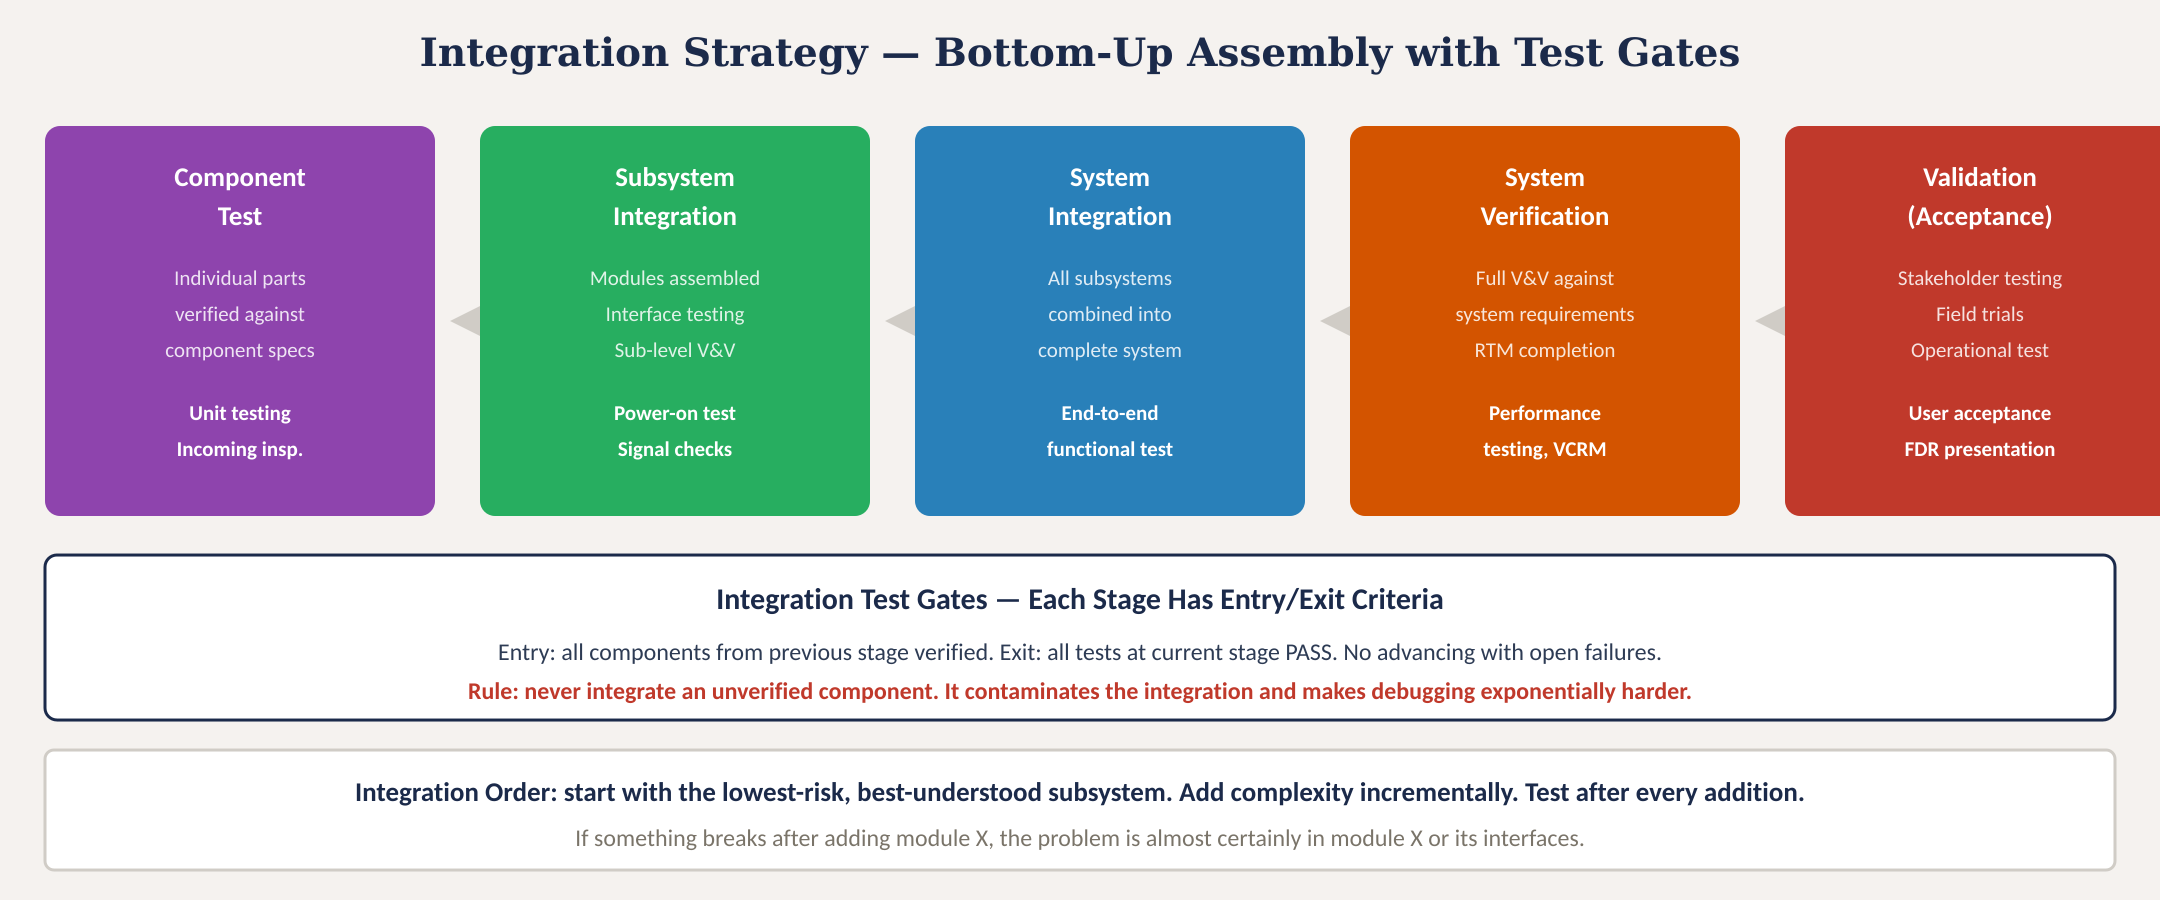
\includegraphics[width=\textwidth]{Subsystem Integration/fig_integration_strategy.png}
\caption{Bottom-up integration with test gates.}\end{figure}

\begin{figure}[ht!]\centering
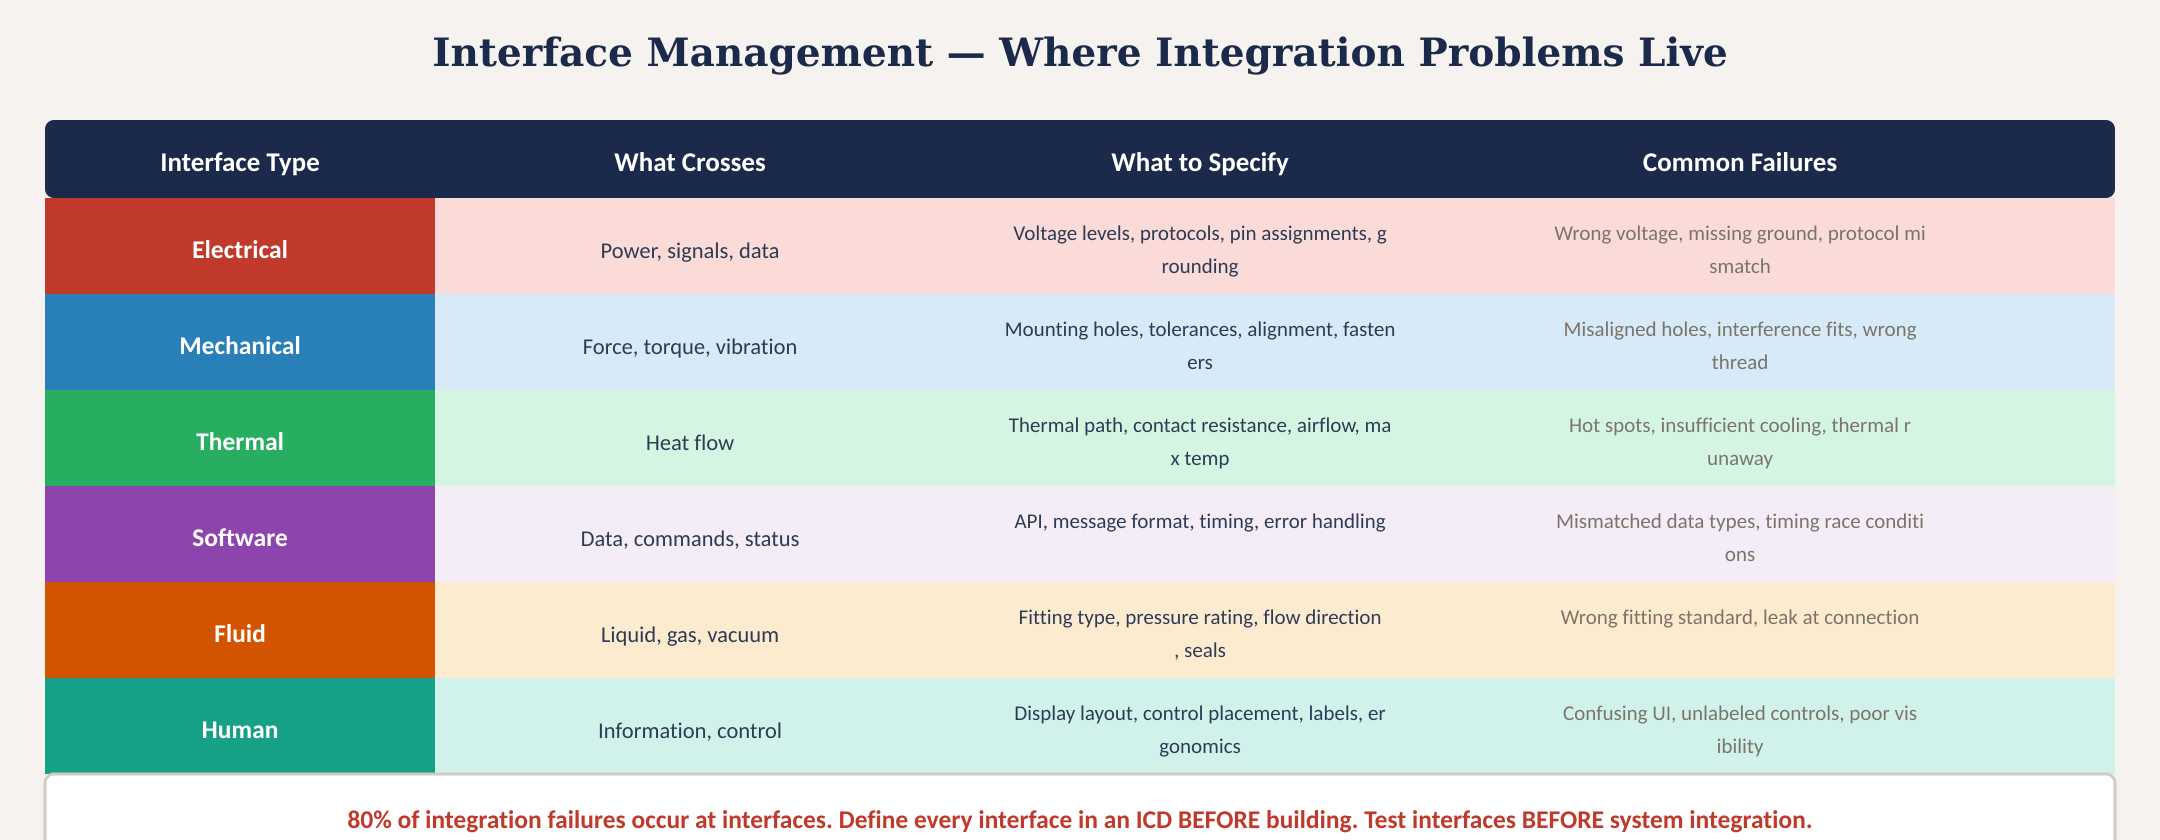
\includegraphics[width=\textwidth]{Subsystem Integration/fig_interface_management.png}
\caption{Interface types and common failure modes.}\end{figure}

\begin{figure}[ht!]\centering
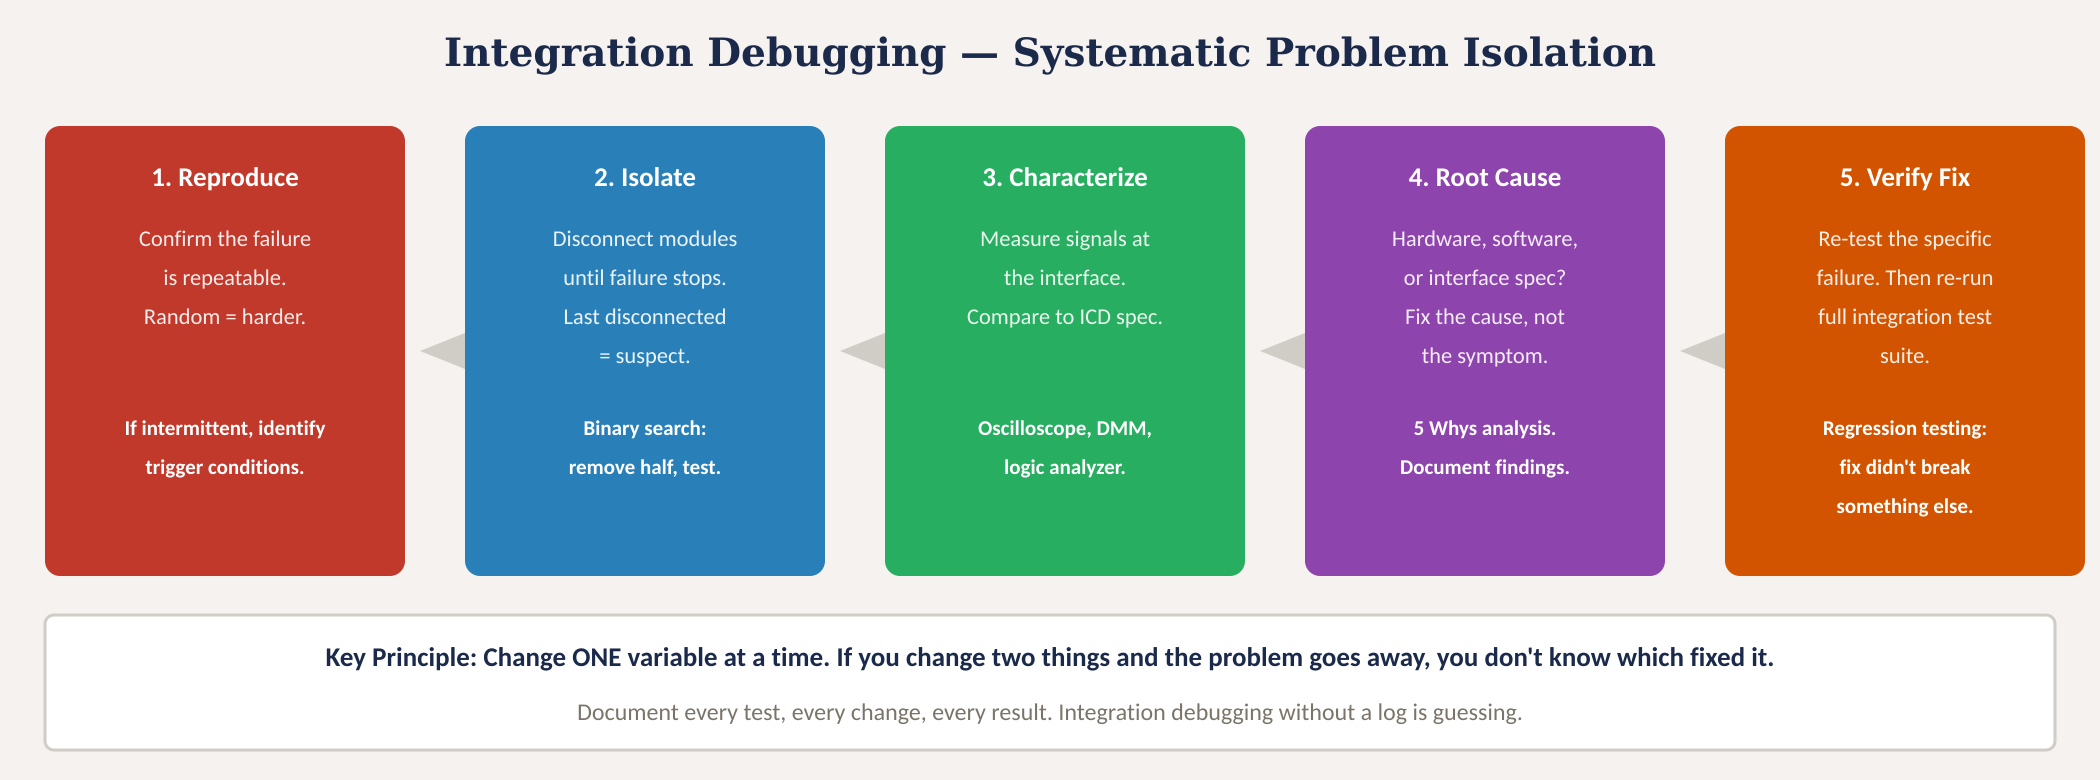
\includegraphics[width=\textwidth]{Subsystem Integration/fig_debugging_process.png}
\caption{Five-step systematic debugging process.}\end{figure}

\begin{figure}[ht!]\centering
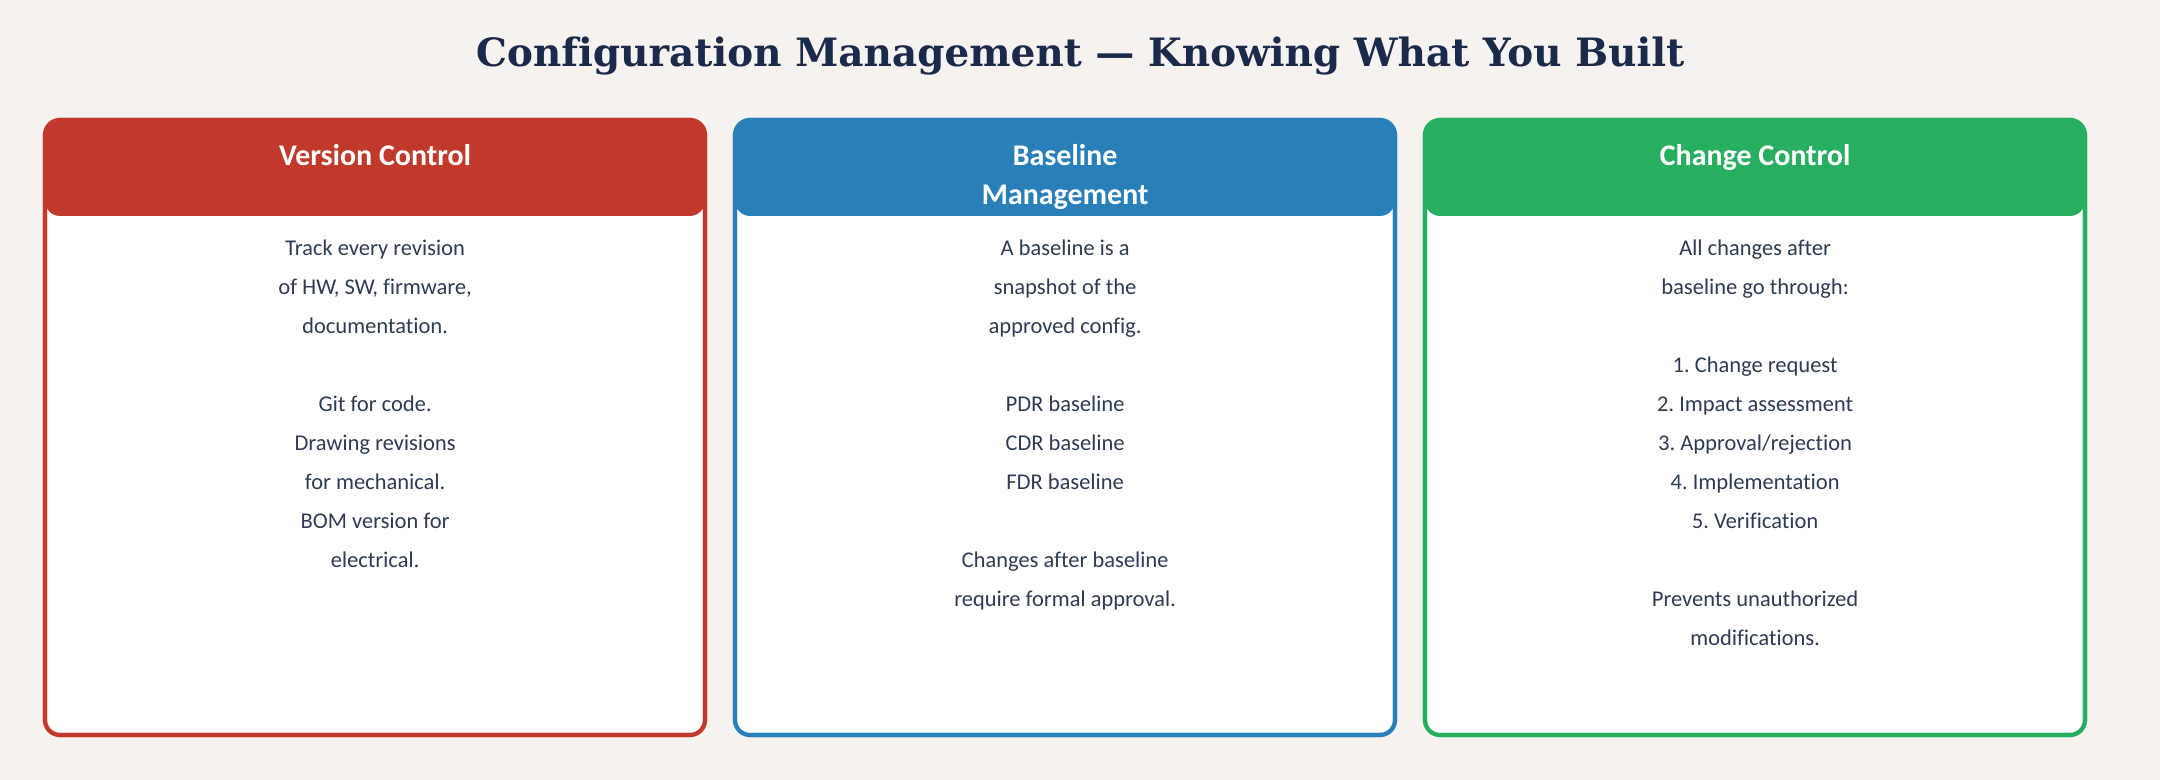
\includegraphics[width=\textwidth]{Subsystem Integration/fig_config_management.png}
\caption{Configuration management pillars.}\end{figure}

\FloatBarrier
\section{Integration Strategy}
\subsection{Bottom-Up Integration}
Verify components individually $\to$ integrate into subsystems $\to$ test each subsystem $\to$ combine into system $\to$ system test. At each stage, add \textbf{ONE new element} and test. If something breaks, the new element or its interface is the prime suspect.

\needspace{4\baselineskip}
\begin{warningbox}[Never Big-Bang]
``Big-bang'' integration---assembling every component at once and powering on---is the fastest route to an undebuggable system. When everything is connected simultaneously and nothing works, you have no information about where the failure is. Bottom-up integration with incremental addition provides \emph{isolation by construction}: the last thing you added is the first thing you investigate.
\end{warningbox}

\subsection{Integration Stages and the V-Model}
Integration stages map directly to the verification levels on the right side of the V-Model:

\begin{center}
\small
\begin{tabularx}{\textwidth}{l X X}
\toprule
\textbf{Integration Stage} & \textbf{V-Model Level} & \textbf{What Is Verified} \\
\midrule
Component testing & Unit test & Individual component meets its specification \\
Subsystem integration & Integration test & Components within a subsystem communicate correctly; subsystem requirements met \\
System integration & System test & All subsystems work together; system requirements met \\
Acceptance testing & Validation & Complete system meets stakeholder's operational needs \\
\bottomrule
\end{tabularx}
\end{center}

Each stage has \textbf{entry criteria} (what must be true before you begin) and \textbf{exit criteria} (what must be demonstrated before you advance). Entry for subsystem integration: all components in the subsystem individually verified. Exit: all subsystem-level tests PASS. Never advance with open failures---they compound at the next level.

\needspace{4\baselineskip}
\begin{tipbox}[Integration Checklist: Before You Connect Anything]
Before connecting subsystem B to subsystem A, verify:
\begin{enumerate}[nosep]
\item Both subsystems individually pass their standalone tests.
\item You have measured the interface signals against the ICD (voltage levels, protocol, pinout).
\item Connector polarity is confirmed (mark pin 1 on both sides with a dot of paint or tape).
\item The power supply can source the combined current draw of both subsystems.
\item You have a known-good rollback point: the last configuration that worked is documented and reproducible.
\end{enumerate}
If any of these are ``no,'' stop. Fix them before proceeding. Skipping entry criteria to ``save time'' always costs more time.
\end{tipbox}

\subsection{Integration Sequence Planning}
The order in which you integrate subsystems matters. Start with the subsystems that have the most interfaces (they affect the most other subsystems) or the highest technical risk (they are most likely to fail). For most electromechanical projects, the integration sequence is: (1)~power supply (everything else depends on it), (2)~controller (the central node), (3)~sensors (simplest interfaces), (4)~actuators (highest power, most failure modes), (5)~communication (can be tested last because it is not required for core function).

\FloatBarrier
\section{Critical Subsystem Demonstrations}
Before attempting full system integration, each critical subsystem must demonstrate that it can perform its allocated functions independently. In MEGN~301, you will identify your two most critical subassemblies, define demonstration goals for each, and demonstrate them to your instructor before proceeding to full system integration (Sprint~4).

A \textbf{critical subassembly} is one that carries the highest technical risk, has the most complex interfaces, or whose failure would prevent the entire system from functioning. For the GreenShield system, the two critical subassemblies might be: (1)~the sensor-controller data acquisition chain (can it read temperature accurately?) and (2)~the relay-heater actuation chain (can it switch the heater reliably?).

\subsection{Planning a Subsystem Demonstration}
For each critical subassembly, define:
\begin{enumerate}[leftmargin=1.5em]
\item \textbf{Demonstration goals}: Specific, measurable outcomes that prove the subassembly works. Not ``show that the sensor works'' but ``demonstrate that the sensor module reads temperature within $\pm 1$\,\degC\ of a reference thermometer at three test points (0\,\degC, 25\,\degC, 50\,\degC).''
\item \textbf{Required hardware and setup}: What physical components, power supplies, test equipment, and fixtures are needed?
\item \textbf{Success criteria}: Binary pass/fail criteria derived from subsystem requirements. If the demonstration does not meet all criteria, document what failed and what modifications are needed.
\item \textbf{Demonstration procedure}: Step-by-step instructions that could be followed by someone unfamiliar with your subsystem.
\end{enumerate}

\subsection{After the Demonstration}
Document the results in a demo report covering: (1)~goals and whether they were met, with specific measured performance values, (2)~any deviations from the proposed procedure, (3)~problems encountered and how they were resolved, and (4)~modifications needed before full system integration. A successful subsystem demonstration is the \textbf{entry criterion} for system integration---do not proceed to full integration until both critical subassemblies have demonstrated their core functionality.

\needspace{4\baselineskip}
\begin{warningbox}[The Demo Trap]
A common student failure is to rush through subsystem demonstrations and declare ``it works'' based on a single successful trial. A subsystem that works once under ideal conditions may fail intermittently under real operating conditions. Run multiple trials, test at boundary conditions (not just room temperature on a benchtop), and document actual measured values---not just ``PASS.''
\end{warningbox}

\FloatBarrier
\section{Interface Management}
80\% of integration failures occur at interfaces. This statistic is consistent across industries, project sizes, and technology domains. It is the single most important fact in systems engineering.

\subsection{Interface Types}
Six types of interfaces exist between subsystems. Every interface in your system falls into at least one category:

\textbf{Electrical}: voltage levels, signal protocols (I$^2$C, SPI, UART, CAN), grounding schemes, current limits, impedance matching, EMI/EMC. The most common failure: logic level mismatch (3.3V vs.\ 5V).

\textbf{Mechanical}: mounting points, tolerances, alignment features, thermal expansion, vibration isolation, fastener specifications. The most common failure: interference fit or misaligned mounting holes.

\textbf{Thermal}: heat flow paths, contact resistance, thermal interface materials, operating temperature limits, heat sinking. The most common failure: component overheating because the thermal path was not designed.

\textbf{Software/Data}: APIs, data formats, message protocols, timing constraints, endianness, byte ordering, error handling. The most common failure: data format mismatch or race condition.

\textbf{Fluid}: fitting types (see Part~II), pressure ratings, flow rates, seal types, material compatibility. The most common failure: leak at a fitting due to incorrect thread type or inadequate tightening.

\textbf{Human}: display visibility, control layout, labeling, ergonomics, error prevention. The most common failure: operator error due to ambiguous or poorly placed controls.

\subsection{The N$^2$ (N-Squared) Diagram}
The N$^2$ diagram is a standard systems engineering tool for systematically identifying and documenting all interfaces between subsystems. It is a square matrix where subsystems are listed along the diagonal. Each off-diagonal cell represents a potential interface: the cell at row~$i$, column~$j$ shows what subsystem~$i$ sends to subsystem~$j$.

\needspace{4\baselineskip}
\begin{keyconceptbox}[GreenShield: N$^2$ Diagram]
\begin{center}\small
\begin{tabular}{l|c|c|c|c|c}
 & \textbf{Sensor} & \textbf{Controller} & \textbf{Relay} & \textbf{Comm} & \textbf{Power} \\
\hline
\textbf{Sensor} & \cellcolor{LightBG}\textbf{Sensor} & I$^2$C temp data & --- & --- & --- \\
\hline
\textbf{Controller} & I$^2$C clock & \cellcolor{LightBG}\textbf{Controller} & GPIO on/off & UART cmd & --- \\
\hline
\textbf{Relay} & --- & Status feedback & \cellcolor{LightBG}\textbf{Relay} & --- & --- \\
\hline
\textbf{Comm} & --- & UART alerts & --- & \cellcolor{LightBG}\textbf{Comm} & --- \\
\hline
\textbf{Power} & 3.3V rail & 5V rail & 12V rail & 3.3V rail & \cellcolor{LightBG}\textbf{Power} \\
\end{tabular}
\end{center}

Reading the diagram: the Sensor sends I$^2$C temperature data to the Controller. The Controller sends a GPIO on/off signal to the Relay. The Power Supply provides voltage rails to every subsystem. Each non-empty off-diagonal cell requires an ICD. Empty cells confirm that no interface exists---this is also valuable information.
\end{keyconceptbox}

\subsection{Interface Control Documents (ICDs)}
An ICD formally specifies everything that crosses a subsystem boundary. For student projects, a complete ICD for an electrical interface should contain:

\begin{center}
\small
\begin{tabularx}{\textwidth}{l X}
\toprule
\textbf{ICD Field} & \textbf{Example (Sensor $\to$ Controller)} \\
\midrule
Interface ID & IF-01 \\
Subsystems & Sensor Module $\leftrightarrow$ Controller \\
Physical connection & 4-pin JST PH connector, P/N B4B-PH-K-S \\
Pinout & Pin 1: VCC (3.3V), Pin 2: GND, Pin 3: SDA, Pin 4: SCL \\
Protocol & I$^2$C, 100\,kHz standard mode \\
Data format & 16-bit signed integer, resolution 0.0625\,\degC/LSB \\
Voltage levels & 3.3V logic, 4.7\,k$\Omega$ pull-ups on SDA and SCL \\
Max current & 1.5\,mA during conversion; 1\,$\mu$A standby \\
Cable & 4-conductor, 26~AWG, max length 30\,cm \\
Owner & Sensor sub-team \\
\bottomrule
\end{tabularx}
\end{center}

Write ICDs \textbf{during architecture definition} (Chapter~2), not during integration. If you wait until integration to discover that two subsystems use incompatible voltage levels, you have an expensive rework problem. The ICD is the contract between sub-teams: if both sides build to the ICD, the interface will work when connected.

\FloatBarrier
\section{Debugging}
When integration reveals a failure, systematic debugging prevents wasted time. Follow this five-step process:

\begin{enumerate}[leftmargin=1.5em]
\item \textbf{Reproduce}: Make the failure happen reliably and consistently. Note the exact conditions: input values, timing, sequence, environmental state. A failure you cannot reproduce is a failure you cannot fix.
\item \textbf{Isolate}: Disconnect modules one at a time until the failure stops. The last module disconnected (or its interface) is the prime suspect. If the failure persists with a single module, the problem is within that module.
\item \textbf{Characterize}: Measure signals at the interface against the ICD specification. Use an oscilloscope for timing and voltage levels, a logic analyzer for digital protocols, a multimeter for power rails. Compare measured values to ICD specifications---any discrepancy is a potential root cause.
\item \textbf{Root-cause}: Is the problem in hardware (wrong component, bad solder joint, miswired connector), software (logic error, timing bug, incorrect register configuration), or the interface specification (ICD is wrong or incomplete)?
\item \textbf{Fix and verify}: Implement the correction. Verify the fix resolves the original failure. Then \textbf{regression-test}: re-run all previously passed tests to confirm the fix did not break anything else.
\end{enumerate}

\textbf{Change ONE variable at a time.} If you change the firmware and swap a component simultaneously, and the problem goes away, you do not know which change fixed it---and the other change may have introduced a new latent defect.

\needspace{4\baselineskip}
\begin{keyconceptbox}[GreenShield: Integration Failure Case Study]
\textbf{Scenario}: The sensor module and controller work individually. When connected, the controller reads temperature as $-127$\,\degC\ (the DS18B20 error code for communication failure).

\textbf{Step 1 (Reproduce)}: Failure occurs every time on power-up. Consistent.

\textbf{Step 2 (Isolate)}: Disconnect sensor cable. Controller reads default value (expected). Reconnect---failure returns. Problem is at the Sensor$\leftrightarrow$Controller interface.

\textbf{Step 3 (Characterize)}: Oscilloscope on I$^2$C lines. SDA and SCL are stuck LOW. ICD specifies 4.7\,k$\Omega$ pull-ups to 3.3V. Measure pull-up resistors: not installed. The sensor module PCB has unpopulated pull-up footprints.

\textbf{Step 4 (Root-cause)}: Interface specification error---the ICD assigned pull-up responsibility to the sensor sub-team, but the sensor PCB was assembled without them. Root cause: BOM for sensor module did not include pull-up resistors.

\textbf{Step 5 (Fix)}: Solder 4.7\,k$\Omega$ pull-ups onto sensor PCB. Re-test: controller reads 22.3\,\degC\ (correct). Regression-test: verify relay actuation, SMS alert, and setpoint adjustment still function. All pass.

\textbf{Lesson}: This failure would have been caught during subsystem testing if the sensor module had been tested against the ICD before integration. The ICD existed but was not used as a test reference.
\end{keyconceptbox}

\FloatBarrier
\section{Configuration Management}
Configuration management ensures that everyone on the team is working with the same, correct version of every artifact---hardware, software, documents, and test data.

Three pillars:

\textbf{Version control}: Git for source code and firmware (branch per feature, merge to main with review). Revision letters for engineering drawings (Rev~A at PDR, Rev~B at CDR, etc.). Versioned BOMs with date stamps. Every file that could change must be under version control.

\needspace{4\baselineskip}
\begin{tipbox}[Version Control for ME Students]
If the command line is intimidating, use a GUI Git client like \textbf{GitHub Desktop} or \textbf{Sourcetree}---they do the same thing with buttons instead of typed commands. For CAD files and hardware drawings that Git handles poorly, use a simple naming convention in a shared Google Drive folder: \texttt{Enclosure\_V3-2\_2026-04-15.SLDPRT}. This is infinitely better than \texttt{Final\_Final\_reallyFinal.SLDPRT}. Whatever system you choose, use it from day one---not the night before CDR.
\end{tipbox}

\textbf{Baseline management}: A baseline is a snapshot of the complete system state at a milestone. PDR baseline, CDR baseline, and FDR baseline capture the requirements, architecture, code, drawings, and BOM at that point. After a baseline is established, \emph{any change requires formal change control}.

\textbf{Change control}: The process for modifying a baselined artifact: (1)~Change request documenting the proposed change and its justification, (2)~Impact assessment on all affected artifacts (does changing this requirement invalidate a test? does changing this pinout require a PCB respin?), (3)~Approval by the configuration control authority (typically the project lead or faculty advisor), (4)~Implementation of the change in all affected artifacts, (5)~Verification that the change works and that previously verified items are re-verified (regression testing).

\needspace{4\baselineskip}
\begin{warningbox}[Regression Testing After Changes]
Any change to a subsystem---firmware update, component substitution, wiring modification---may invalidate prior verification results. After making a change, you must re-run all tests affected by that change. This is \textbf{regression testing}. Without it, you may fix one problem and silently introduce three others. The VCRM should track which requirements need re-verification after each change.
\end{warningbox}

\needspace{4\baselineskip}
\begin{keyconceptbox}[Case Study: Diagnosing the Brown-Out Blues]
\textbf{Symptom}: Your microcontroller resets every time the motor starts. The system works fine without the motor connected.

\textbf{Reproduce}: Power the system, command motor start $\to$ MCU resets (brown-out detected on serial monitor). 100\% reproducible.

\textbf{Isolate}: Disconnect the motor. System runs indefinitely. Reconnect the motor with a separate benchtop supply $\to$ no reset. The problem is the shared power path, not the motor itself.

\textbf{Characterize}: Measure the 5\,V MCU rail with an oscilloscope during motor start. The rail dips to 3.1\,V for 50\,ms as the motor draws 8\,A inrush through the shared wire. The MCU's brown-out threshold is 3.3\,V.

\textbf{Root-cause}: Star grounding violation. The motor's return current flows through the same ground wire as the MCU, creating a voltage drop ($V = I \times R_{\text{wire}}$). Combined with insufficient bulk capacitance on the MCU rail, the transient pulls the MCU below its operating voltage.

\textbf{Fix}: (1)~Add a 1000\,$\mu$F electrolytic capacitor on the MCU rail to absorb the transient. (2)~Run separate power and ground wires from the supply to the motor (star topology, Chapter~9). (3)~Verify the fix: motor starts without MCU reset. (4)~Regression test: re-run all sensor and communication tests to confirm nothing else changed.

This is the most common integration failure in student projects. The fix costs \$0.50 and ten minutes---but only if you measure with an oscilloscope instead of guessing.
\end{keyconceptbox}

\FloatBarrier
\section{Artifact Handoff: What Chapter~5 Produces}

\begin{center}
\small
\begin{tabularx}{\textwidth}{l X X}
\toprule
\textbf{Artifact from Ch.~5} & \textbf{Primary Contents} & \textbf{Used Directly In\ldots} \\
\midrule
Integration test results & Subsystem and system test data, pass/fail & VCRM update (Ch.~4), FDR evidence \\
Updated ICDs & Revised interface specs from integration findings & Maintenance documentation (Ch.~6) \\
Discrepancy reports & Interface failures, root causes, corrective actions & Lessons learned, configuration management \\
Configuration baselines & FDR-baseline BOM, firmware version, drawings & Maintenance and spare parts (Ch.~6) \\
N$^2$ diagram (verified) & All interfaces confirmed operational & System documentation \\
\bottomrule
\end{tabularx}
\end{center}

\needspace{4\baselineskip}
\begin{tipbox}[Industry SE Parallels]
This chapter corresponds to INCOSE SEH Section~4.5.3 (Integration) and NASA SP-2016-6105 Section~5.4 (Product Integration). The N$^2$ diagram is a standard tool described in NASA SP-2016-6105 Section~4.4.1. Configuration management follows the principles of ANSI/EIA-649 (Configuration Management Standard) and is described in INCOSE SEH Section~4.8. In industry, integration testing is typically preceded by a Test Readiness Review (TRR) and followed by a System Verification Review (SVR) before the system proceeds to acceptance testing.
\end{tipbox}

\FloatBarrier
\section{Practice Questions}
Questions are tiered: \textbf{C} = Comprehension, \textbf{A} = Application, \textbf{CT} = Critical Thinking.
\begin{enumerate}[leftmargin=1.5em]
\item \textbf{[A]} Your system works with subsystems A and B connected, but fails when you add subsystem C. Describe your debugging approach step by step using the five-step process.
\item Draw an N$^2$ diagram for a system with a sensor module, controller board, motor driver, and power supply. Identify all interfaces. Which interfaces are highest risk and why?
\item Your teammate changes the firmware without telling anyone and the system stops working. What configuration management failure occurred? What process should have been followed?
\item Write entry and exit criteria for the subsystem integration stage of a greenhouse monitoring system.
\item Write a complete ICD (all fields from the template in this chapter) for the interface between a motor driver subsystem and a controller board that uses PWM speed control.
\item Explain why regression testing is necessary after fixing an integration defect. Give a concrete example where a fix to one subsystem could break a previously verified capability in another subsystem.
\item A system has four subsystems and six interfaces. The team has two weeks for integration. Propose an integration sequence with justification, and identify which interface you would test first and why.
\end{enumerate}

\subsection{Answers}
\begin{enumerate}[leftmargin=1.5em]
\item (1) Reproduce: confirm failure happens consistently with A+B+C connected. Document symptoms. (2) Isolate: disconnect C, verify A+B still works. Reconnect C's power but not its signal lines---does it fail? If yes, C is loading the power supply. If no, reconnect signal lines one at a time. (3) Characterize: measure signals at the C interface with an oscilloscope. Compare to ICD specs. Look for voltage level mismatches, missing pull-ups, excessive current draw, timing violations. (4) Root-cause: determine whether C's hardware is faulty, C's firmware has a bug, or the ICD between B and C is incorrect. (5) Fix the root cause, verify the fix, then re-test A+B and A+B+C to confirm nothing else broke.

\item N$^2$ diagram has sensor, controller, motor driver, power on the diagonal. Interfaces: Sensor$\to$Controller (analog/digital temp data), Controller$\to$Motor Driver (PWM + direction signals), Power$\to$All (voltage rails), Motor Driver$\to$Controller (fault/status feedback). Highest risk: Controller$\to$Motor Driver (high-power switching near low-power logic creates EMI, ground bounce, and potential latch-up) and Power$\to$Motor Driver (motor stall current may exceed power supply capacity, causing voltage droop that resets the controller).

\item Two configuration management failures: (1) No version control---the firmware change was not committed with a version number and change log. (2) No change control---changes to baselined artifacts (post-CDR firmware) require a change request, impact assessment, and approval before implementation. Correct process: file a change request, assess impact on all subsystems, get approval, implement with a new version number, test the change, regression-test all affected functions, update the VCRM.

\item Entry criteria: all four subsystem modules (sensor, controller, relay, comm) individually verified per their subsystem test procedures; all ICDs reviewed and approved; integration test procedures written and reviewed; test equipment calibrated; team briefed on integration sequence. Exit criteria: all subsystem-to-subsystem interfaces verified per ICD specifications; all system-level test procedures executed with PASS verdicts; VCRM updated with all system requirement statuses; no open Severity-1 discrepancy reports.

\item ICD example --- Motor Driver $\leftrightarrow$ Controller: Interface ID: IF-03. Subsystems: Controller $\leftrightarrow$ Motor Driver. Connector: 6-pin Molex Mini-Fit Jr., P/N 39-01-2060. Pinout: Pin 1: PWM (3.3V logic, 20\,kHz, 0--100\% duty cycle), Pin 2: DIR (3.3V logic, HIGH=forward), Pin 3: EN (3.3V logic, HIGH=enabled), Pin 4: FAULT (open-drain output, active LOW, 10\,k$\Omega$ pull-up to 3.3V), Pin 5: GND (power ground), Pin 6: GND (signal ground). Protocol: Hardware PWM, no software handshake. Max current: 20\,mA per signal pin; motor power on separate connector. Cable: 6-conductor, 22~AWG, max 50\,cm, twisted pairs for PWM/GND and FAULT/GND. Owner: Motor driver sub-team.

\item A fix to the motor driver firmware (changing PWM frequency to reduce audible noise) could shift the EMI spectrum and cause the sensor module's ADC readings to become noisy, failing the temperature accuracy requirement that was previously verified. Without regression testing, this new failure remains latent until the next time someone checks temperature accuracy---which may be at FDR, when it is too late to fix cleanly.

\item Integration sequence: (1) Power supply first---all other subsystems depend on it; test output voltage regulation and current capacity. (2) Controller second---central communication hub; verify boot sequence and self-test. (3) Sensor third---simplest interface (I$^2$C), low risk; verify data acquisition. (4) Motor driver fourth---highest power interface, most EMI risk; verify PWM control and fault detection. Test the Power$\to$Motor Driver interface first because motor stall current is the most likely cause of system-level power issues, and a voltage droop during motor start could reset the controller and corrupt sensor data.
\end{enumerate}

\FloatBarrier
\chapter{Operations \& Maintenance}

\vspace{1em}

This chapter extends the systems engineering lifecycle beyond the V-Model into the operational phase---the longest and most expensive period of a system's life. Operations and maintenance (O\&M) is not an afterthought; it is the phase where the system delivers value to the stakeholder, and where the quality of every earlier design decision is ultimately judged. A system that works perfectly on the test bench but cannot be maintained, repaired, or eventually retired is not a successful engineering product.

\needspace{4\baselineskip}
\begin{keyconceptbox}[Bottom Line]
O\&M is 50--70\% of lifecycle cost, and 80\% of that cost is locked in by your early design decisions. Design for Access, Modularity, Diagnostics, and Standardization \emph{during} Chapters~2--3, not after FDR. Use the FMECA to mathematically justify which components need preventive maintenance. For your Final Design Report, your Quick-Start Guide should enable your instructor to operate the system, and your maintenance appendix should include a spare parts list and FMECA results.
\end{keyconceptbox}

\vspace{1em}

\begin{figure}[ht!]\centering
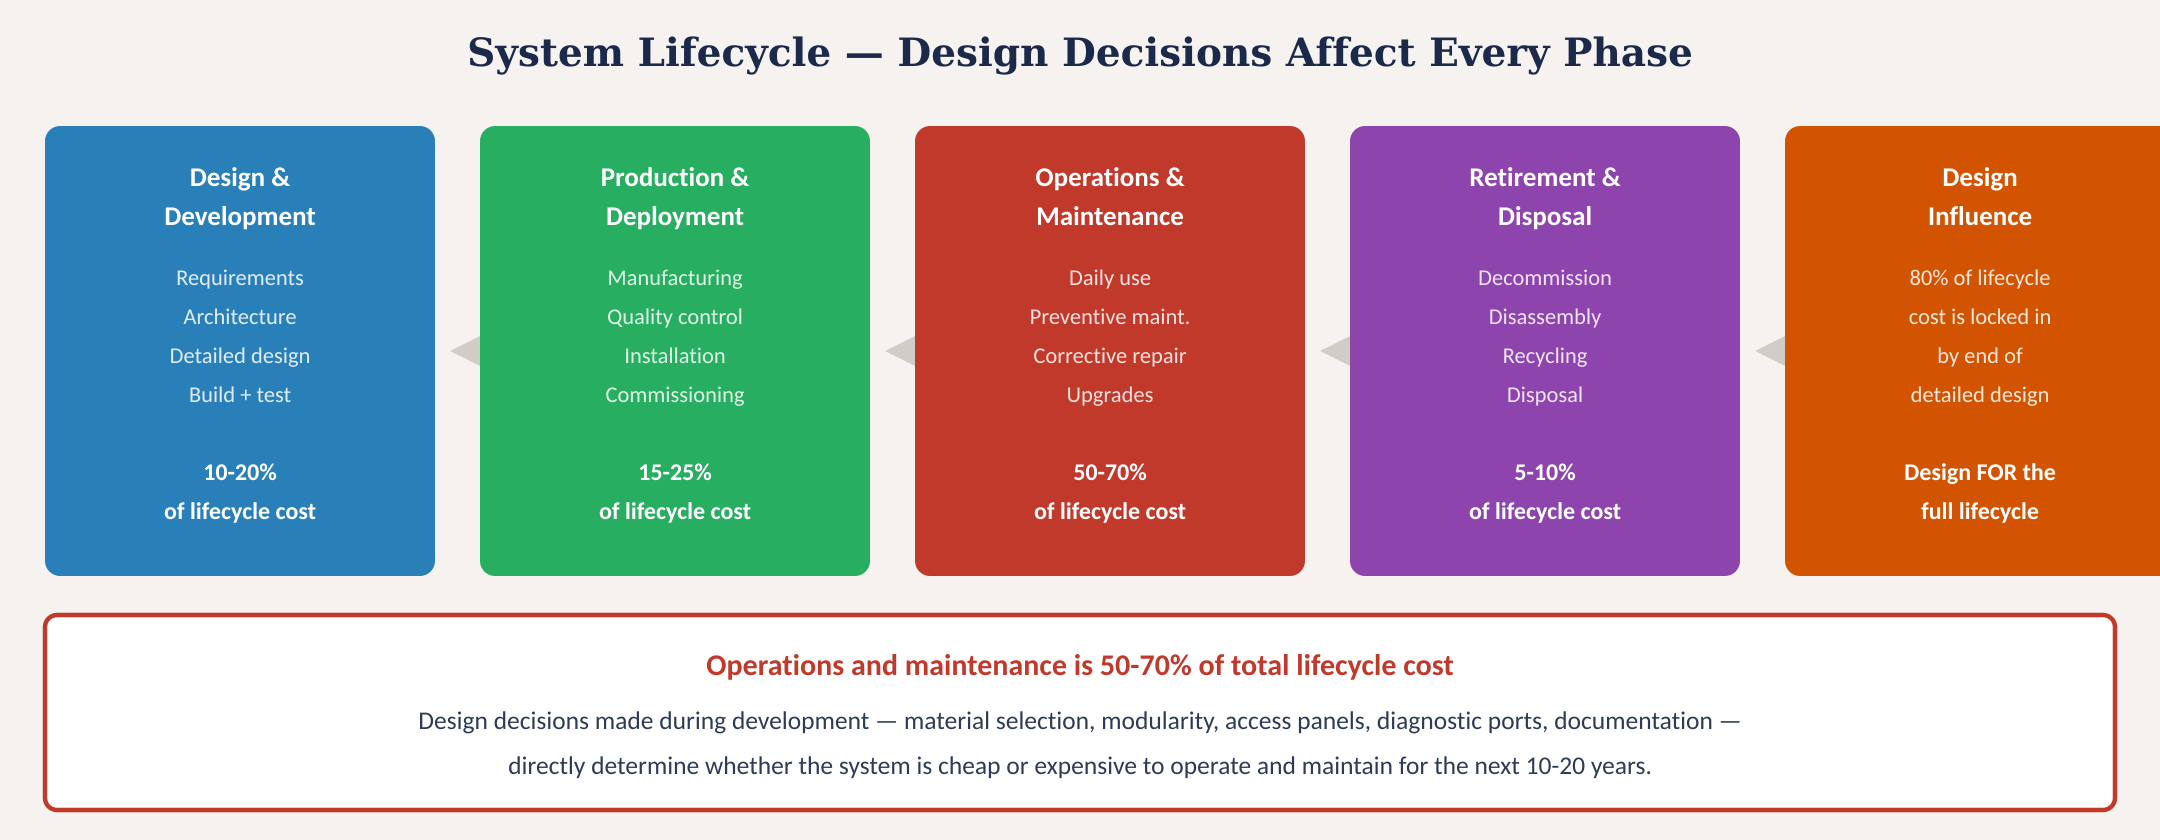
\includegraphics[width=\textwidth]{Ops and Maintenance/fig_system_lifecycle.png}
\caption{System lifecycle with cost distribution.}\end{figure}

\begin{figure}[ht!]\centering
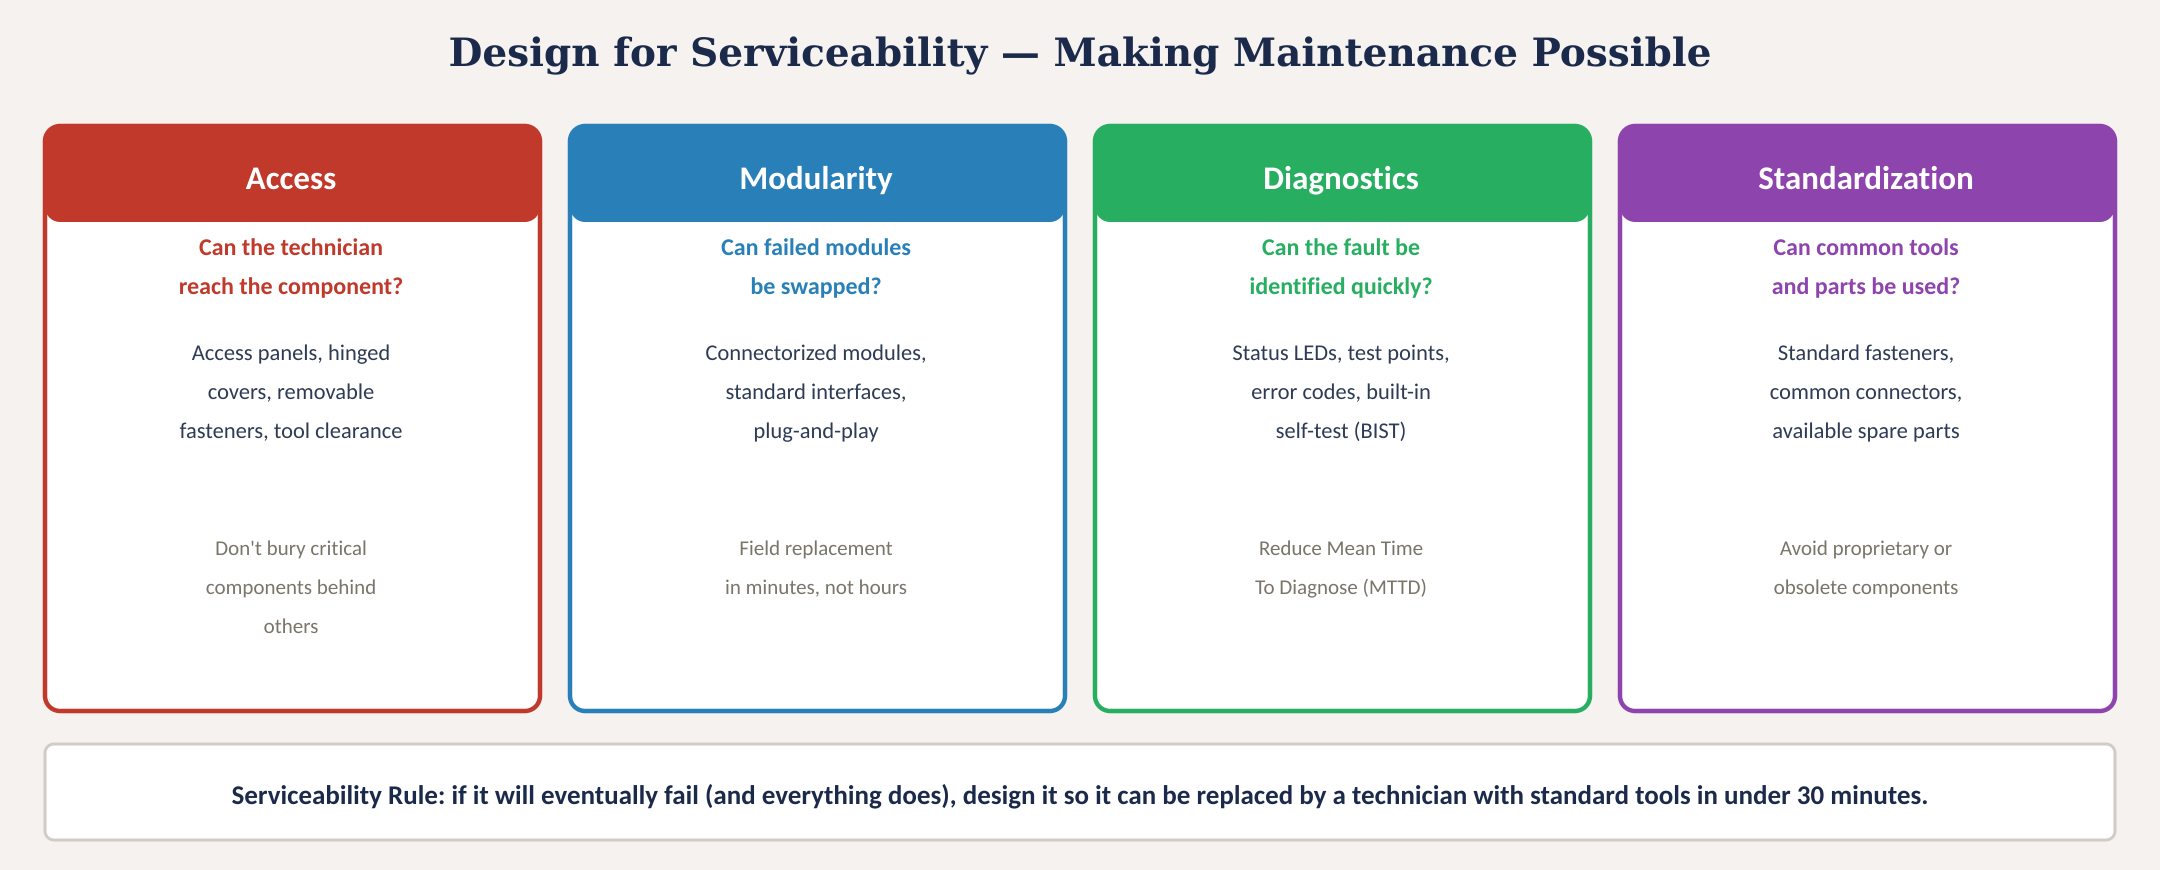
\includegraphics[width=\textwidth]{Ops and Maintenance/fig_serviceability.png}
\caption{Four serviceability principles.}\end{figure}

\begin{figure}[ht!]\centering
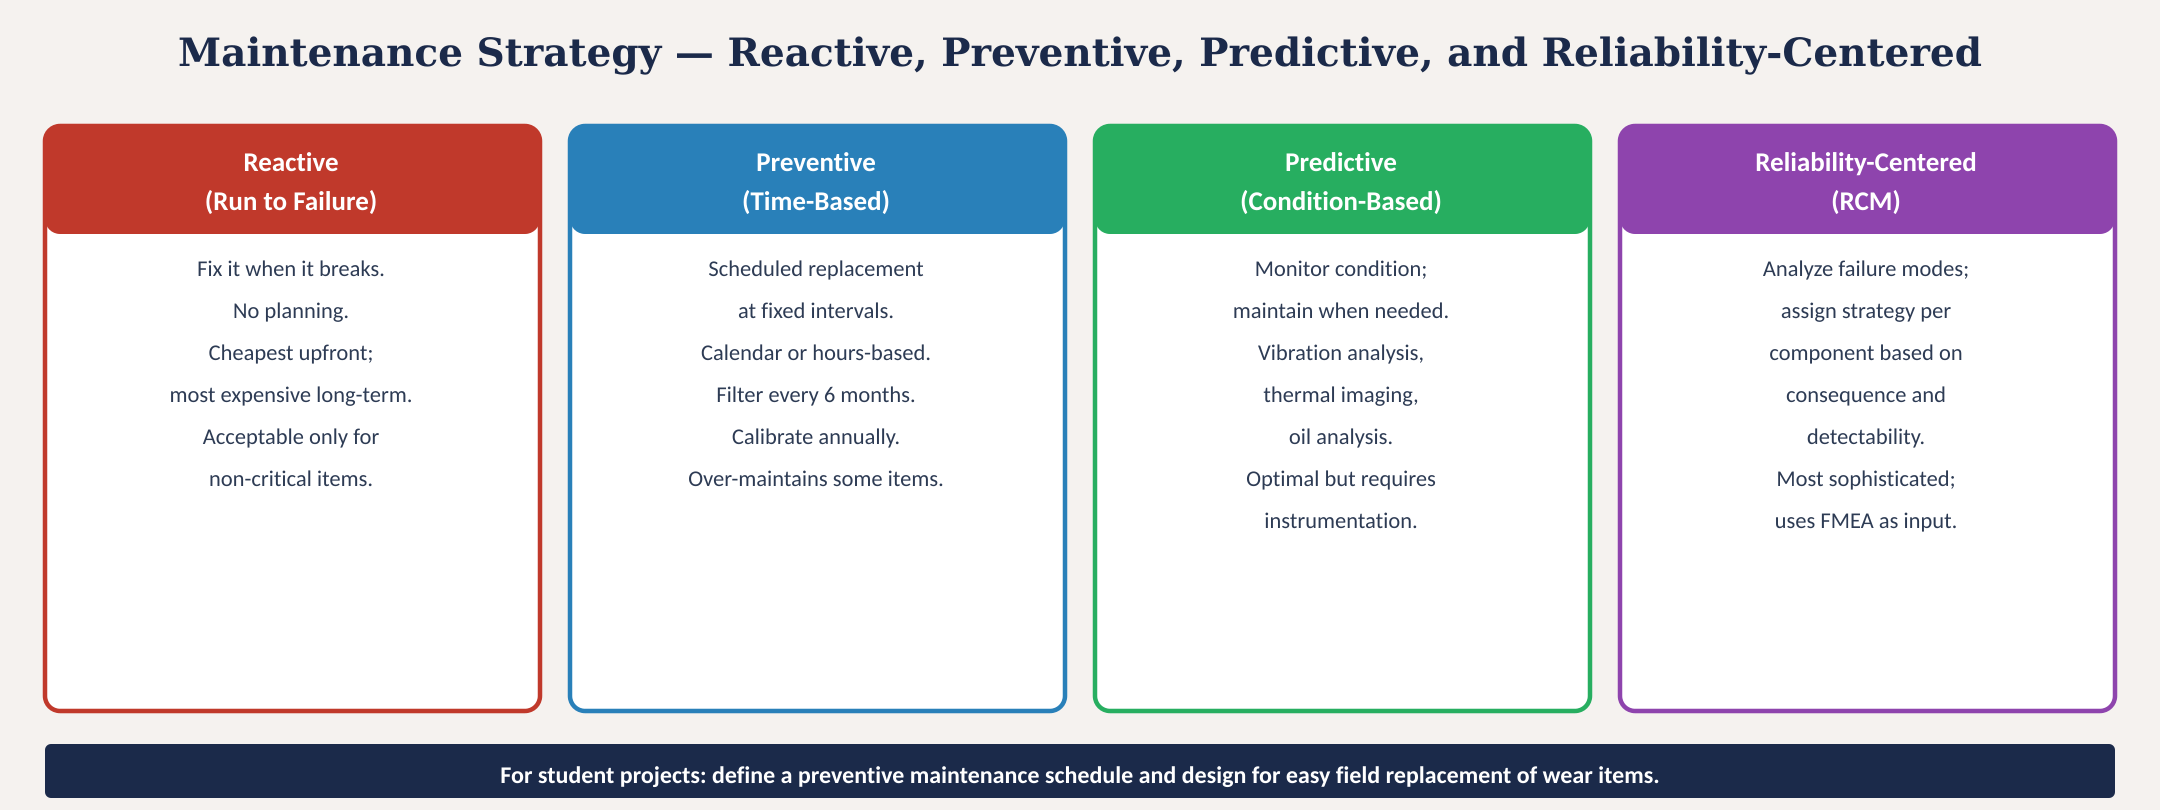
\includegraphics[width=\textwidth]{Ops and Maintenance/fig_maintenance_strategies.png}
\caption{Maintenance strategies from reactive to RCM.}\end{figure}

\begin{figure}[ht!]\centering
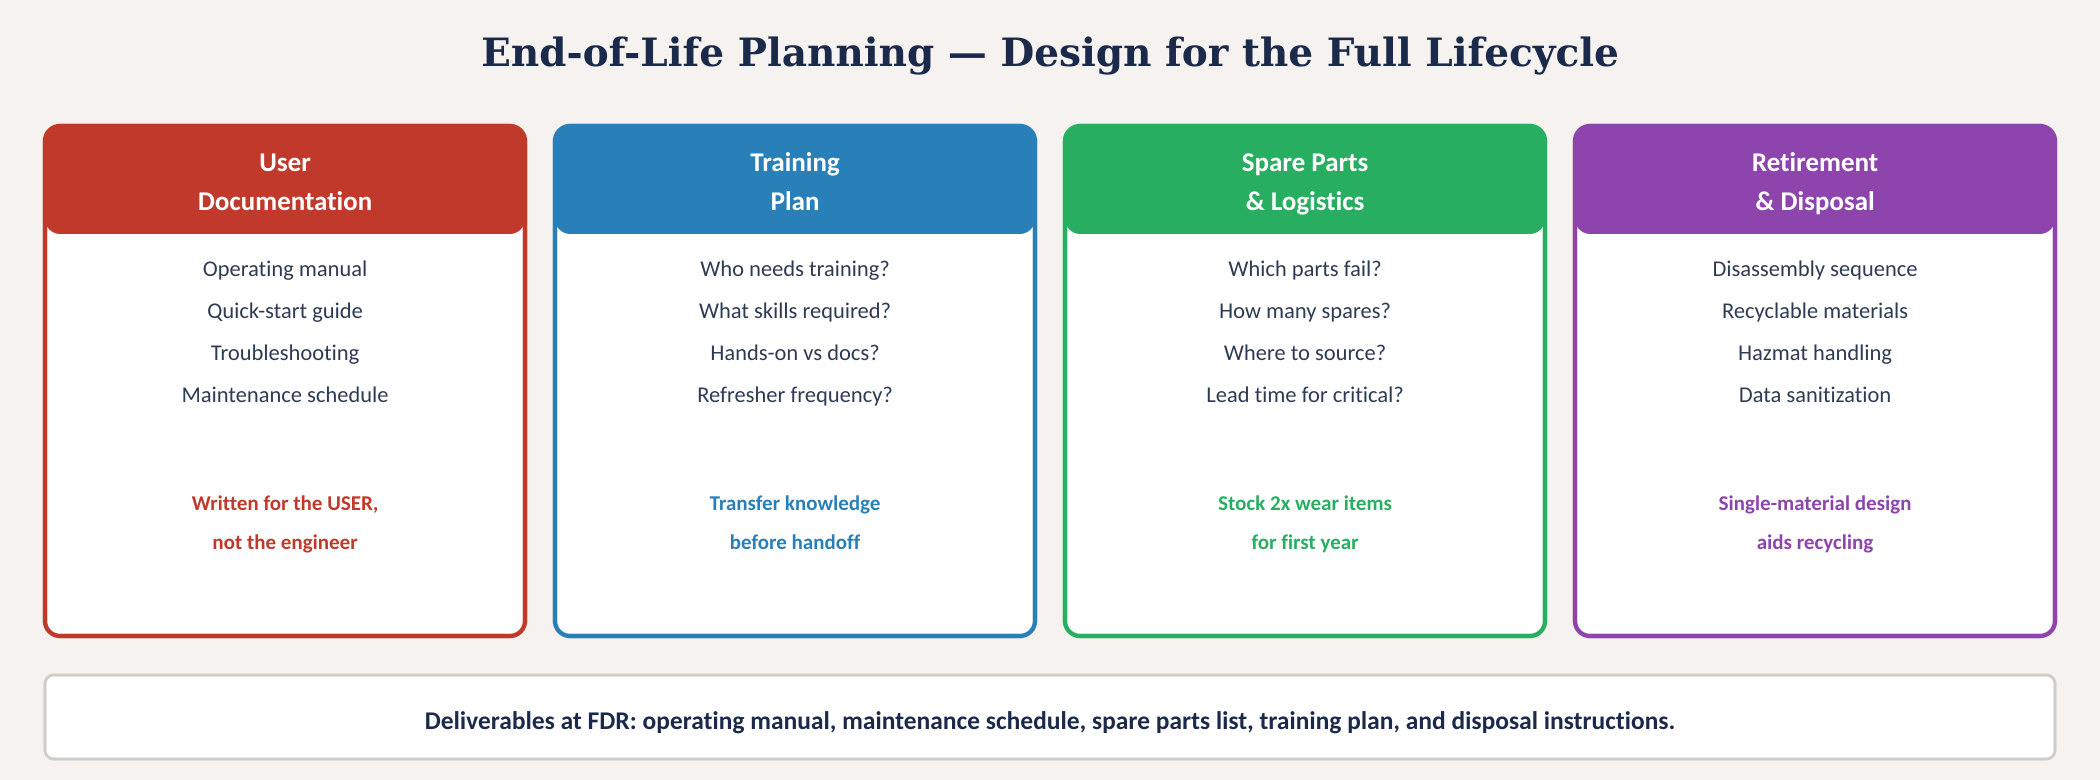
\includegraphics[width=\textwidth]{Ops and Maintenance/fig_eol_planning.png}
\caption{End-of-life planning deliverables.}\end{figure}

\FloatBarrier
\section{Lifecycle Thinking}
Operations and maintenance accounts for 50--70\% of total lifecycle cost---far more than development. Yet 80\% of that cost is locked in by decisions made during concept and preliminary design, when the team has the most freedom and the least information. This paradox---that the decisions with the greatest lifecycle impact are made earliest, with the least data---is one of the central challenges of systems engineering.

The practical implication is clear: design-for-serviceability, maintainability, reliability, and disposability must be considered \emph{during design} (Chapters~2--3), not after the system is built and deployed. Every architecture decision, component selection, and interface design carries a maintenance consequence. Choosing a soldered connection instead of a connector saves \$0.50 in production but adds 30 minutes of labor and a soldering iron to every field repair. Choosing a proprietary sensor saves 2 weeks of development time but creates a single-source dependency that may strand the system when the vendor discontinues the part.

\FloatBarrier
\section{Reliability Engineering Fundamentals}

\subsection{The Bathtub Curve}
The failure rate of most engineered systems follows a characteristic pattern known as the \textbf{bathtub curve}, which has three distinct phases:

\textbf{Phase 1: Infant Mortality} (decreasing failure rate). Failures occur early due to manufacturing defects, assembly errors, weak components, and latent defects that escaped quality control. In industry, this phase is addressed through ``burn-in'' testing: operating the system under stress for a defined period to force early failures before delivery. For student projects, your first few hours of operation often reveal soldering defects, loose connectors, and firmware bugs.

\textbf{Phase 2: Useful Life} (constant, low failure rate). After infant mortality issues are resolved, the system enters its useful life with a roughly constant failure rate. Failures in this phase are random and not predictable for individual units, though the \emph{rate} is statistically predictable across a population. This is the phase described by MTBF.

\textbf{Phase 3: Wear-Out} (increasing failure rate). Components reach the end of their useful life. Bearings wear, seals degrade, capacitors dry out, batteries lose capacity. These failures are predictable and preventable through scheduled replacement---the basis of preventive maintenance.

Understanding which phase a component is in determines the correct maintenance strategy. Preventive replacement during Phase~2 is wasteful (you are replacing working parts). Reactive maintenance during Phase~3 is negligent (you are waiting for predictable failures to cause damage).

\subsection{Reliability Metrics}
\textbf{MTBF (Mean Time Between Failures)}: The average operating time between failures for a repairable system. A system with MTBF = 2000 hours does not mean it will last exactly 2000 hours---it means that over many operating cycles, the average time between failures is 2000 hours. MTBF is a statistical measure, not a guarantee.

\textbf{MTTR (Mean Time To Repair)}: The average time to diagnose, repair, and restore a failed system to operation. MTTR is driven by design decisions: access to components, modularity, diagnostic capability, spare parts availability, and documentation quality.

\textbf{Availability}: The fraction of time the system is operational:
\[
A = \frac{\text{MTBF}}{\text{MTBF} + \text{MTTR}}
\]

For example, a system with MTBF = 2000\,hr and MTTR = 24\,hr has $A = 2000/(2000+24) = 0.988$, or 98.8\% availability. This sounds good---but it means the system is down for roughly 105 hours per year. Moving to 99.9\% availability (``three nines'') reduces downtime to about 9 hours per year. ``Five nines'' (99.999\%) means less than 6 minutes of downtime per year---a requirement so stringent it demands redundant hardware, automatic failover, and 24/7 monitoring. The distance between 99\% and 99.999\% is not a minor improvement; it is an entirely different class of engineering. For MEGN~301 projects, targeting 95--99\% availability is realistic. Improving MTTR through better serviceability design is often cheaper and faster than improving MTBF through better components. Halving MTTR from 24\,hr to 12\,hr raises availability to $2000/2012 = 0.994$ (99.4\%), while doubling MTBF to 4000\,hr only reaches $4000/4024 = 0.994$---the same result, but typically at far greater cost.

\subsection{FMECA: Failure Modes, Effects, and Criticality Analysis}
The FMECA is a systematic method for identifying potential failure modes, assessing their effects on system performance, and prioritizing them for design action. It is the primary tool for translating reliability concerns into concrete design improvements.

For each component or function, the FMECA asks three questions: (1)~How can this fail? (failure mode), (2)~What happens when it fails? (effect on system), and (3)~How bad is it? (criticality). The output is a ranked list of failure modes that drives design decisions, maintenance strategies, and spare parts planning.

\subsubsection{The Risk Priority Number (RPN)}
Each failure mode is scored on three scales (each rated 1--10):

\textbf{Severity (S)}: How serious is the effect if this failure occurs? (1 = no effect; 10 = safety hazard or complete system loss)

\textbf{Occurrence (O)}: How likely is this failure mode? (1 = extremely unlikely; 10 = almost certain)

\textbf{Detection (D)}: How likely is the failure to be detected before it causes harm? (1 = certainly detected; 10 = undetectable)

\[
\text{RPN} = S \times O \times D
\]

RPN ranges from 1 to 1000. Higher RPN values indicate higher priority for corrective action. A common threshold for action is RPN $\geq 100$, though this varies by industry and application. \textbf{Important}: RPN is a \emph{ranking} tool, not a linear measurement. Because it is the product of three ordinal scales, an RPN of 200 is not ``twice as bad'' as an RPN of 100---it simply ranks higher in the prioritization queue (e.g., an RPN drop from 200 to 100 does not mean the risk is ``50\% better,'' only that it is now lower in the priority queue). Use RPN to sort your failure modes from most to least critical and to allocate your limited design effort accordingly, but do not attempt to calculate percentage improvements or ratios between RPN values.

\needspace{4\baselineskip}
\begin{keyconceptbox}[GreenShield: FMECA Fragment]
\begin{center}\small
\begin{tabularx}{\textwidth}{X l l l l X}
\toprule
\textbf{Failure Mode} & \textbf{S} & \textbf{O} & \textbf{D} & \textbf{RPN} & \textbf{Action} \\
\midrule
Temp sensor reads high (frost not detected) & 9 & 3 & 5 & 135 & Add redundant sensor; implement plausibility check \\
Relay welds closed (heater cannot turn off) & 8 & 2 & 4 & 64 & Add thermal fuse in series; monitor heater current \\
SMS module loses network & 5 & 4 & 2 & 40 & Autonomous local control; retry logic \\
Power supply fails & 9 & 2 & 3 & 54 & Add UPS / battery backup for 4\,hr operation \\
\bottomrule
\end{tabularx}
\end{center}

The highest-RPN failure (sensor reading high, RPN = 135) receives the most attention: a redundant sensor and software plausibility check are added to the design. Notice that the relay welding failure has high severity (8) but low RPN (64) because it is unlikely (O = 2) and somewhat detectable (D = 4). The FMECA provides a mathematical basis for allocating limited design resources to the failures that matter most.
\end{keyconceptbox}

\FloatBarrier
\section{Design for Serviceability}
Four design principles that reduce MTTR and improve field maintainability:

\textbf{Access}: Can the technician physically reach the component that needs service? Design with access panels, hinged covers, quick-release fasteners. Allow tool clearance around fasteners (minimum two wrench lengths). Place high-replacement-rate components at the system exterior, not buried behind three other subsystems.

\textbf{Modularity}: Can a failed module be swapped in the field without specialized equipment? Design with connectorized interfaces (not soldered wires), independently testable modules (each module can be bench-tested before installation), and standardized mechanical mounting (so a replacement module from inventory fits without modification).

\textbf{Diagnostics}: Can the fault be identified without disassembly? Provide status LEDs on each subsystem, accessible test points at key interfaces, error codes displayed on the operator interface, and Built-In Self-Test (BIST) routines that the system runs at power-up or on command.

\textbf{Standardization}: Can common tools and commercially available parts be used? Specify standard fastener sizes (minimize the number of wrench sizes needed). Use multi-source components (not sole-source or proprietary). Design for common hand tools rather than specialized fixtures.

\subsection{Writing Maintainability Requirements}
Maintainability is not a vague aspiration---it is a set of quantitative requirements that should be defined in Chapter~2 alongside functional and performance requirements. Examples:

\begin{itemize}[leftmargin=1.5em]
\item ``A trained technician shall be able to replace the temperature sensor module within 15 minutes using only a Phillips screwdriver and a 10\,mm wrench.''
\item ``The system shall provide a visual fault indication (LED or display message) within 10 seconds of detecting a sensor communication failure.''
\item ``All field-replaceable modules shall be connectorized with keyed connectors that prevent incorrect installation.''
\item ``The system shall achieve an availability of $\geq 99\%$ based on MTBF $\geq 2000$\,hr and MTTR $\leq 2$\,hr.''
\end{itemize}

These requirements are testable (Chapter~4) and traceable to stakeholder needs (the operator needs the system to be available during frost-risk periods). They also drive design decisions: the 15-minute sensor replacement requirement dictates that the sensor must be accessible, connectorized, and mounted with quick-release hardware.

\needspace{4\baselineskip}
\begin{keyconceptbox}[GreenShield: O\&M Requirement Trace]
\textbf{Stakeholder need} (Ch.~1): ``I can't afford to lose a night of protection while waiting for a repair.''

\textbf{O\&M requirement} (Ch.~2): ``SYS-REQ-20: A trained operator shall be able to replace any single failed field-replaceable unit and restore system operation within 30 minutes.''

\textbf{Design implication} (Ch.~3): Sensor module designed with quick-disconnect JST connector, DIN-rail clip mount, no tools required for removal.

\textbf{Verification} (Ch.~4): Maintenance procedure test---give a trained operator a spare sensor module and time the replacement.

\textbf{Maintenance plan} (Ch.~6): Spare sensor module included in field kit; replacement interval = on-failure (Phase~2 random failure).
\end{keyconceptbox}

\FloatBarrier
\section{Maintenance Planning}
Four strategies, listed in order of increasing sophistication and decreasing long-term cost:

\textbf{Reactive (run-to-failure)}: No scheduled maintenance. Replace or repair only when the system fails. Cheapest upfront but most expensive long-term because unplanned downtime occurs at the worst possible moment. Appropriate only for non-critical components with low replacement cost and no safety implications.

\textbf{Preventive (time-based)}: Replace components at fixed intervals based on expected life, regardless of condition. Replaces components that may still have useful life remaining (wasteful) but prevents unplanned failures. Appropriate for wear-out items with well-characterized lifetimes (belts, filters, seals, batteries).

\textbf{Predictive (condition-based)}: Monitor component health indicators (vibration, temperature, current draw, degradation trends) and replace only when indicators cross a threshold. More efficient than preventive because it uses actual condition rather than calendar time. Requires sensors and monitoring infrastructure.

\textbf{Reliability-Centered Maintenance (RCM)}: Uses FMECA results to assign the optimal maintenance strategy to each component based on its failure mode, consequence, and detectability. Different components in the same system may receive different strategies. RCM is the most sophisticated approach and is standard in aerospace, nuclear, and critical infrastructure.

For student projects: define a \textbf{preventive schedule} for all wear items and design for \textbf{easy field replacement}. Identify all wear items (bearings, seals, belts, batteries, filters), define replacement intervals based on manufacturer data or engineering estimates, create a spare parts list with vendor part numbers and lead times, and establish a calibration schedule for all sensors.

\FloatBarrier
\section{Documentation, Training, and End-of-Life}
Four documentation deliverables, each serving a different audience and purpose:

\needspace{4\baselineskip}
\begin{tipbox}[Mapping to Your Final Design Report]
For your MEGN~301 Final Design Report: Section~1 (Design Requirements) should reference your SDRD and VCRM results. Section~2 (Design Process) should contain your design evolution with photos. Section~3 (Hazards Discussion) should present your FMEA results and risk mitigations. Section~4 (Future Work) should include your maintenance recommendations. The Appendix should contain your Quick-Start Guide, spare parts list, and any remaining FMECA or test data. Write these documents \emph{as you go}---do not attempt to reconstruct them the night before submission.
\end{tipbox}

\textbf{Quick-Start Guide} (1 page): Enables a new operator to set up and start the system within 10 minutes. Numbered steps, photographs, no assumptions about prior knowledge. This is the document that accompanies the system when it leaves your hands.

\begin{tipbox}[Quick-Start Guide Template]
Your Quick-Start Guide must include these six elements, each with a photograph:
\begin{enumerate}[nosep]
\item \textbf{Unbox and verify}: List all components; photo of laid-out contents.
\item \textbf{Physical setup}: Mount/position the system; connect cables; photo of correct configuration.
\item \textbf{Power up}: Plug in or switch on; expected LED/display behavior on startup.
\item \textbf{Configure}: Set user-adjustable parameters (setpoints, times, modes).
\item \textbf{Operate}: Walk through one complete operating cycle in normal mode.
\item \textbf{Verify it works}: A simple self-test the operator performs to confirm the system is functioning (e.g., ``Press TEST---relay clicks, heater activates for 5 seconds, display shows OK'').
\end{enumerate}
If your instructor cannot follow your Quick-Start Guide and have the system running in 10 minutes without asking you a single question, the guide is not finished.
\end{tipbox}

\textbf{Operating Manual} (complete reference): Organized by task rather than by subsystem. Covers every operating mode, every user-adjustable parameter, every status indication. Includes a troubleshooting section organized by symptom (``display shows ERR-03'' $\to$ ``sensor communication failure; see Section~4.2'').

\textbf{Maintenance Manual}: Step-by-step procedures for every maintenance task, with photographs showing hand positions, tool usage, and component orientation. Includes a complete spare parts list with part numbers, vendors, and quantities.

\textbf{Troubleshooting Guide}: Symptom-based flowcharts that lead the maintainer from an observed problem to a root cause and corrective action. Organized as decision trees: ``Is the status LED on? Yes $\to$ go to Step~3. No $\to$ check power supply.''

\subsection{Training Plan}
Identify three audiences: \textbf{operators} (daily users who need to run the system), \textbf{maintainers} (technicians who need to repair and calibrate it), and \textbf{trainers} (people who will train future operators and maintainers after your team is gone). For each audience, define training methods (hands-on demonstration, written procedures, video walkthroughs) and competency assessment (can they independently perform the required tasks?).

\subsection{Knowledge Transfer and Design Rationale}
The most perishable artifact in any engineering project is the \emph{rationale} for design decisions. Document why decisions were made, not just what was decided. Record known limitations, workarounds, and gotchas. Future maintainers will encounter situations your team did not anticipate, and the design rationale gives them the context to make good decisions.

\subsection{End-of-Life Planning}
Design for disassembly: use fasteners rather than adhesives, minimize material types for recyclability, label materials. Identify and plan for hazardous materials: batteries (lithium recycling programs), solvents, lead-containing components. Plan for data sanitization if the system stores user data or configuration settings.

\FloatBarrier
\section{Artifact Handoff: What Chapter~6 Produces}

\begin{center}
\small
\begin{tabularx}{\textwidth}{l X X}
\toprule
\textbf{Artifact from Ch.~6} & \textbf{Primary Contents} & \textbf{Purpose} \\
\midrule
FMECA table & Failure modes, RPNs, mitigation actions & Drives maintenance strategy and spare parts \\
Maintenance schedule & Wear items, intervals, procedures & Operational planning \\
Spare parts list & Part numbers, vendors, quantities, lead times & Logistics and inventory \\
Documentation suite & Quick-start, ops manual, maintenance manual, troubleshooting & Operator and maintainer support \\
Training plan & Audiences, methods, competency criteria & Knowledge transfer \\
End-of-life plan & Disassembly, recycling, hazmat handling & Responsible disposal \\
\bottomrule
\end{tabularx}
\end{center}

\needspace{4\baselineskip}
\begin{tipbox}[Industry SE Parallels]
This chapter corresponds to INCOSE SEH Section~4.7 (Operation) and~4.8 (Maintenance and Disposal). FMECA follows MIL-STD-1629A and IEC~60812. The bathtub curve is a fundamental concept in reliability engineering described in IEC~60300 (Dependability Management). Reliability-Centered Maintenance (RCM) is codified in SAE~JA1011. In industry, the maintenance plan and FMECA are typically deliverables reviewed at the Production Readiness Review (PRR) or as part of the Integrated Logistics Support (ILS) package.
\end{tipbox}

\FloatBarrier
\section{Practice Questions}
Questions are tiered: \textbf{C} = Comprehension, \textbf{A} = Application, \textbf{CT} = Critical Thinking.
\begin{enumerate}[leftmargin=1.5em]
\item \textbf{[A]} A system has MTBF = 2000 hrs and MTTR = 24 hrs. Calculate availability. Propose two design changes to improve availability, one targeting MTBF and one targeting MTTR. Calculate the new availability for each.
\item Write a quick-start guide (1 page, numbered steps) for a greenhouse temperature monitoring system. Include safety precautions and a ``verify it works'' step.
\item Your project sponsor asks why you budgeted \$200 for spare parts on a \$2000 project. Justify the expenditure using lifecycle cost arguments and the availability equation.
\item Identify all wear items in an electromechanical system with a DC motor, belt drive, pressure sensor, and lithium battery. Define replacement intervals for each and justify your choice of maintenance strategy (reactive, preventive, or predictive) for each item.
\item A DC motor in your system has the following failure mode: bearing seizure. Rate this failure mode for Severity (1--10), Occurrence (1--10), and Detection (1--10). Calculate the RPN. Propose a design change that reduces the RPN by at least 50\% and explain which factor(s) your change addresses.
\item Explain the three phases of the bathtub curve. For each phase, give a concrete example of a failure that would occur in an electromechanical greenhouse control system, and state the appropriate maintenance strategy for that phase.
\item Construct a partial FMECA table (at least four failure modes) for a battery-powered outdoor sensor node. Calculate RPNs and identify which failure modes exceed the action threshold of RPN $\geq 100$.
\item Why is reducing MTTR often more cost-effective than increasing MTBF? Use the availability equation to show numerically that halving MTTR has a greater effect on availability than doubling MTBF for a system with MTBF = 1000\,hr and MTTR = 50\,hr.
\end{enumerate}

\subsection{Answers}
\begin{enumerate}[leftmargin=1.5em]
\item $A = 2000/(2000+24) = 0.9881$ or 98.81\%. Targeting MTBF: upgrade to industrial-grade components with screened reliability data, increasing MTBF to 4000\,hr. New $A = 4000/4024 = 0.9940$ (99.40\%). Targeting MTTR: redesign for modular replacement with connectorized subsystems, pre-diagnosed fault codes, and a spare parts kit on-site, reducing MTTR to 4\,hr. New $A = 2000/2004 = 0.9980$ (99.80\%). The MTTR improvement yields higher availability at likely lower cost---confirming that serviceability design is usually more cost-effective than component upgrades.

\item Quick-Start Guide: (1) Unbox system; verify all components against packing list (controller, sensor probe, relay module, power adapter, mounting hardware). (2) Mount controller box inside greenhouse at eye level using provided screws. (3) Insert sensor probe through access grommet; position probe at plant canopy height, at least 30\,cm from walls and heat sources. (4) Connect sensor cable to controller (keyed connector---only fits one way). (5) Connect heater control cable from relay module to heater power cord (follow wiring diagram). \textbf{Safety}: disconnect heater from mains before connecting relay. (6) Plug power adapter into mains outlet. (7) Verify startup: controller display shows current temperature within 60 seconds. Press ``Test'' button---relay clicks, heater activates for 5 seconds. (8) Set frost threshold using UP/DOWN buttons (default: 3\,\degC). (9) System is operational. Monitor for 24 hours and verify SMS alert during first frost event.

\item A \$200 spare parts budget is 10\% of the project cost and provides insurance against downtime. Without spares, a single \$15 sensor failure could leave the system non-operational for 1--2 weeks (component lead time), during which frost events cause crop losses of \$500+/event. The spare parts kit (backup sensor, spare relay, fuses, connectors) costs \$200 and reduces MTTR from weeks (order and wait) to hours (swap from kit). Using the availability equation: without spares, effective MTTR = 336\,hr (2 weeks); $A = 2000/2336 = 0.856$ (85.6\%). With spares, MTTR = 2\,hr; $A = 2000/2002 = 0.999$ (99.9\%). The \$200 investment raises availability from 86\% to 99.9\%.

\item Wear items: (a) DC motor brushes---preventive replacement at 2000\,hrs (manufacturer specification); brushes are a well-characterized wear-out item. (b) Belt---preventive replacement at 1500\,hrs or upon visible cracking/stretching; belts fatigue and degrade with UV and heat. (c) Pressure sensor diaphragm---predictive (monitor zero-drift trend); diaphragms degrade slowly and failure is detectable before total loss. (d) Lithium battery---preventive replacement at 2 years or when capacity drops below 80\% (manufacturer cycle-life data); battery degradation is calendar- and cycle-dependent. The motor bearings (not listed but present) should be monitored predictively via vibration or noise increase.

\item Bearing seizure: Severity = 8 (motor stops, system loses actuation capability; not a safety hazard if thermal fuse is present). Occurrence = 3 (unlikely in normal operating conditions with proper lubrication; more likely if dusty environment or overloaded). Detection = 6 (bearing noise may be masked by ambient noise; no built-in monitoring). RPN = $8 \times 3 \times 6 = 144$. Design change: add a motor current monitoring circuit that detects the increased current draw preceding seizure (current rises as bearing friction increases). This improves Detection from 6 to 2, reducing RPN to $8 \times 3 \times 2 = 48$---a 67\% reduction.

\item Phase 1 (Infant Mortality): cold solder joint on the relay driver transistor causes intermittent failure during the first week of operation. Strategy: burn-in testing---run the system under load for 48 hours before deployment; inspect all solder joints. Phase 2 (Useful Life): random firmware crash due to a cosmic-ray-induced bit flip in RAM after 8 months of operation. Strategy: watchdog timer resets the controller automatically; reactive maintenance (restart if it occurs). Phase 3 (Wear-Out): relay contact degradation after 100,000 cycles (approximately 3 years of daily cycling) causes increased contact resistance and eventual failure to switch. Strategy: preventive replacement at 80,000 cycles (80\% of rated life).

\item Outdoor sensor node FMECA: (a) Battery depletion in cold weather: S=7, O=5, D=3, RPN=105 ($>$100, action required---add low-battery alert and oversized battery). (b) Antenna connector corroded: S=6, O=3, D=6, RPN=108 ($>$100---specify sealed SMA connector and conformal coating). (c) Enclosure seal cracked by UV: S=8, O=3, D=5, RPN=120 ($>$100---use UV-stabilized EPDM gasket, add UV shield). (d) Sensor drift over temperature: S=5, O=4, D=4, RPN=80 ($<$100---monitor with periodic calibration check, no immediate design change needed).

\item With MTBF = 1000\,hr and MTTR = 50\,hr: baseline $A = 1000/1050 = 0.9524$ (95.24\%). Doubling MTBF to 2000\,hr: $A = 2000/2050 = 0.9756$ (97.56\%), an improvement of 2.32 percentage points. Halving MTTR to 25\,hr: $A = 1000/1025 = 0.9756$ (97.56\%), the same improvement. However, if we halve MTTR further to 12.5\,hr: $A = 1000/1012.5 = 0.9877$ (98.77\%). Doubling MTBF again to 4000\,hr: $A = 4000/4050 = 0.9877$---same result. The diminishing returns are symmetric, but in practice reducing MTTR is cheaper because it involves design changes (access panels, connectors, diagnostics) rather than component upgrades (more expensive parts, redundancy, derating). MTTR reductions also compound with spare parts availability, training, and documentation quality.
\end{enumerate}


\part{Technical Reference}

\FloatBarrier
\chapter{Electrical \& Fluid Connectors}

% ── Title Block ───────────────────────────────────────────────────────


\vspace{1em}

% ── Learning Outcomes ─────────────────────────────────────────────────



\vspace{1em}

% ══════════════════════════════════════════════════════════════════════
\FloatBarrier
\section{Electrical Connectors}
% ══════════════════════════════════════════════════════════════════════

\subsection{Connector Anatomy}

Every electrical connector consists of three fundamental elements:

\begin{enumerate}[leftmargin=1.5em]
  \item \textbf{Contacts} --- The conductive pins (male) and sockets (female) that carry electrical current. Typical base metals are phosphor bronze and beryllium copper (BeCu), plated with either gold (best corrosion resistance, lowest contact resistance) or tin (lower cost, adequate for benign environments).

  \item \textbf{Housing} --- The insulating body that mechanically positions and electrically isolates the contacts. Common housing materials include:
  \begin{itemize}[nosep]
    \item Nylon (PA66) --- general purpose, good toughness, low cost.
    \item PBT (polybutylene terephthalate) --- higher stiffness, better chemical resistance.
    \item LCP (liquid crystal polymer) --- highest temperature rating, used in reflow-soldered connectors.
  \end{itemize}

  \item \textbf{Termination} --- The mechanical and electrical joint between the wire conductor and the contact. The five major termination methods are detailed in Section~\ref{sec:termination}.
\end{enumerate}

\subsection{Gender Convention}

\begin{itemize}[leftmargin=1.5em]
  \item \textbf{Male} (plug/header): pins protrude from the connector face.
  \item \textbf{Female} (receptacle/socket): pins are received into sockets.
  \item In wire-to-wire assemblies, one cable carries the plug, the other the receptacle.
  \item In wire-to-board applications, the board-mounted header is typically male.
\end{itemize}

\subsection{Keying and Polarization}

Connectors use physical features to ensure correct mating orientation and prevent damage from incorrect insertion. Common keying methods include key slots, asymmetric housing profiles, color coding, and differentiated contact arrangements.

\needspace{4\baselineskip}
\begin{warningbox}[Design Rule]
Always specify keyed connectors when your design has multiple similar-looking connections. Incorrect mating can destroy components, and in student projects this is one of the most common causes of electrical failure on first power-up.
\end{warningbox}


\subsection{Connection Types}

Electrical connectors are classified by \emph{what} they connect:

\begin{table}[ht!]
\centering
\small
\begin{tabularx}{\textwidth}{l X X}
  \toprule
  \textbf{Type} & \textbf{Description} & \textbf{Typical Examples} \\
  \midrule
  Wire-to-Wire & Joins two discrete wires or cable harnesses. Both sides are free-hanging connectors. &
    Molex Mini-Fit Jr., JST SM, Deutsch DT, automotive weatherpacks \\[4pt]
  Wire-to-Board & Connects a wire harness to a printed circuit board (PCB). One side is a cable connector; the other is soldered to the board. &
    JST XH/PH, Molex KK 254, pin headers with crimp housings \\[4pt]
  Board-to-Board & Connects two PCBs directly, often in stacked or mezzanine configurations. No wires involved. &
    Board-to-board headers, mezzanine connectors, card-edge connectors \\
  \bottomrule
\end{tabularx}
\caption{Electrical connector classification by connection type.}
\end{table}

\begin{figure}[ht!]
\centering
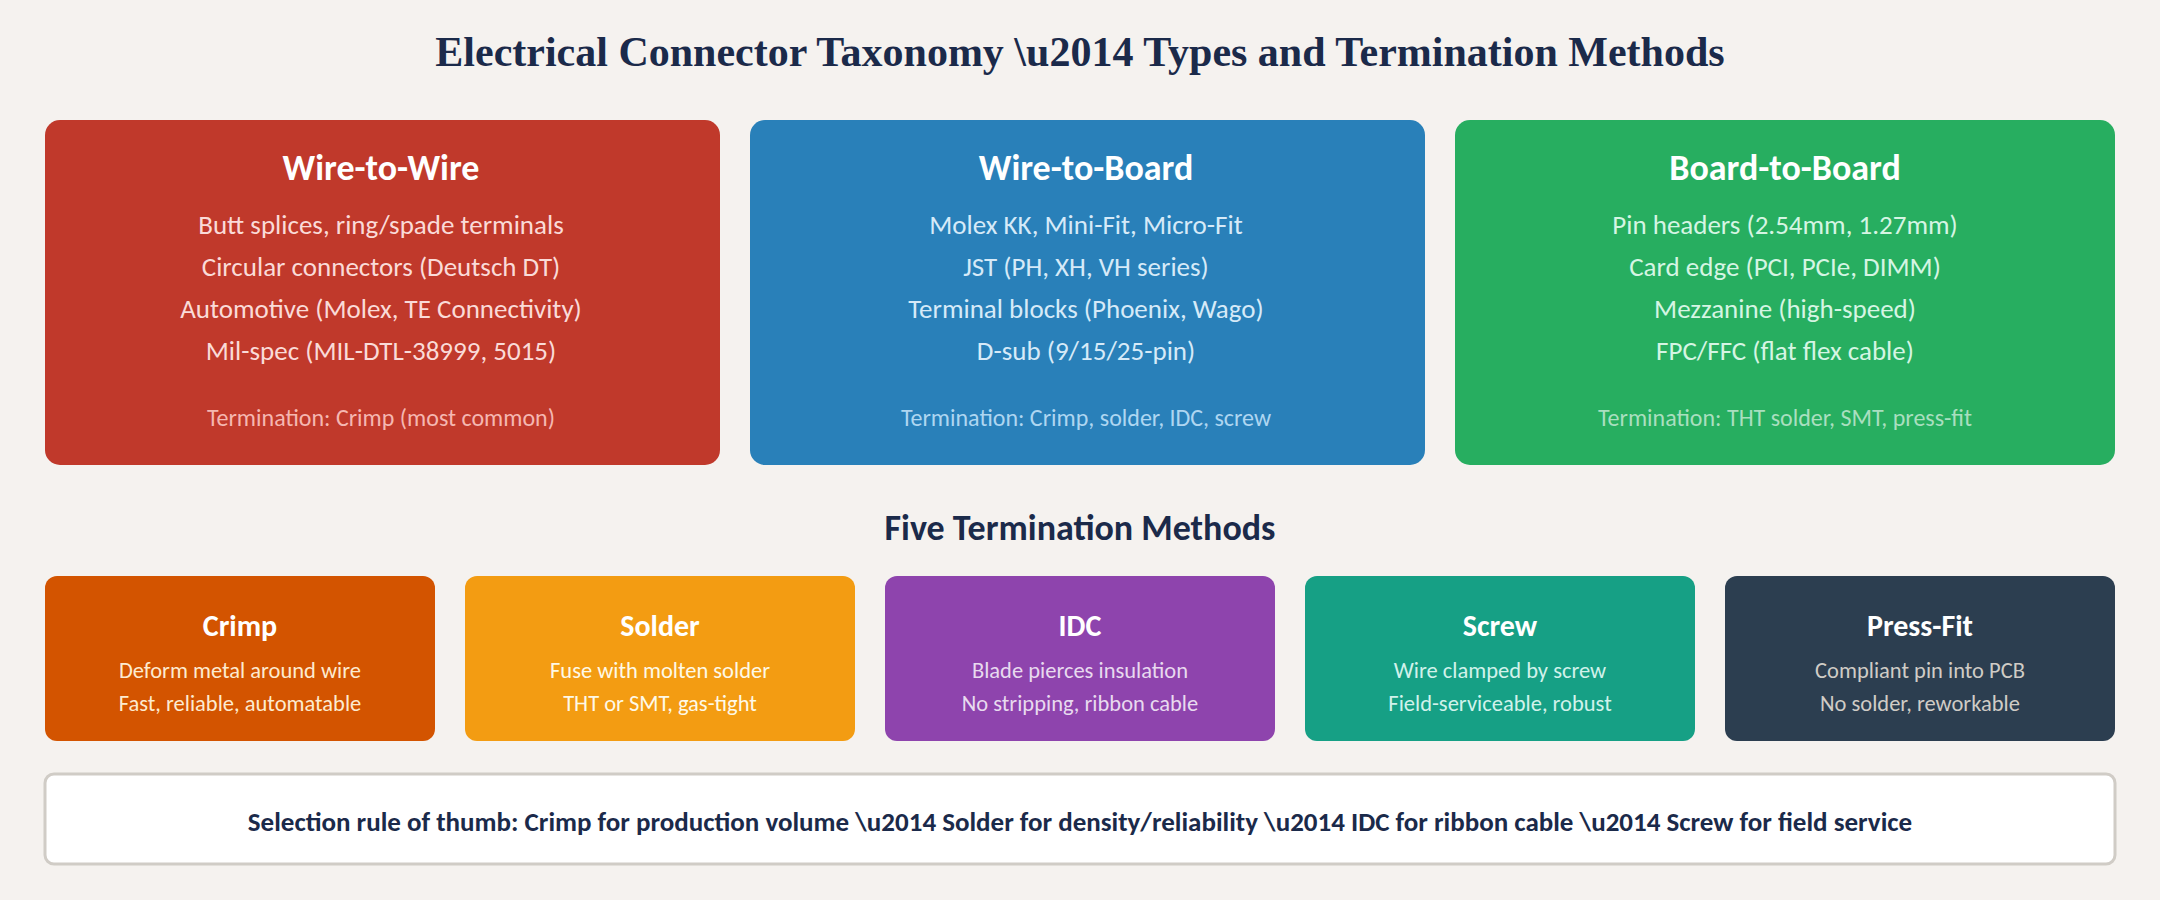
\includegraphics[width=\textwidth]{Electrical and Fluid Connectors/fig1_connector_taxonomy.png}
\caption{Electrical connector taxonomy by connection type with five termination methods~[1],~[2].}
\label{fig:connector_taxonomy}
\end{figure}

\subsection{Harsh-Environment Connectors}

Students designing vehicle harnesses, outdoor systems, or launch hardware will encounter connectors engineered for abuse. Understanding the physical components of these systems is essential for specifying them correctly.

\textbf{Deutsch DT / DTM Series} (automotive/off-highway): These use a wedgelock that mechanically retains all contacts simultaneously, independent of the wire seal. Each cavity receives a silicone wire seal that grips the insulation OD, providing IP67/IP69K protection. Contacts are stamped-and-formed with a barrel crimp --- the crimp must capture both the conductor and the insulation for strain relief. Deutsch connectors are the de facto standard for SAE Baja, Formula SAE, and agricultural equipment harnesses.

\textbf{MIL-DTL-38999 Series III} (aerospace/defense): A bayonet-coupled circular connector with a self-locking coupling ring that resists vibration. Uses machined contacts (not stamped) with interference-fit rear grommets for environmental sealing. Rated for extreme vibration (per MIL-STD-810), wide temperature ranges ($-65$ to $+200$\,\degC), and EMI shielding via conductive shell-to-shell contact. If your design involves launch hardware, flight systems, or classified defense work, 38999 is the starting point.

\textbf{Common to both}: Proper barrel crimps are critical --- the crimp must form a gas-tight cold weld in the conductor barrel \emph{and} a secure grip in the insulation barrel. Using generic pliers instead of a calibrated ratchet tool produces crimps that look acceptable but fail under vibration or thermal cycling.


\subsection{Termination Methods}
\label{sec:termination}

The termination method is how the wire conductor is mechanically and electrically bonded to the connector contact. Each method involves different tools, skill levels, and performance characteristics.

\subsubsection{Crimp}

A precision die compresses a metal barrel around a stripped wire conductor, creating a gas-tight joint through cold-welding at the metal interface.

\begin{itemize}[nosep,leftmargin=1.5em]
  \item \textbf{Strengths}: Fast, repeatable, no heat required, excellent vibration resistance, gas-tight joint resists corrosion.
  \item \textbf{Limitations}: Requires calibrated crimp tools (hand ratchet or pneumatic); die must match the contact exactly. Poor crimps are invisible failures.
  \item \textbf{Best for}: Production wiring, automotive harnesses, harsh-environment connectors.
  \item \textbf{Quality verification}: Pull-test a sample of crimps per IPC/WHMA-A-620. Cross-section crimps periodically to verify cold-weld zone.
\end{itemize}

\needspace{4\baselineskip}
\begin{warningbox}[Pin Extraction: Use the Right Tool]
In prototype environments, students inevitably insert a contact into the wrong cavity. \textbf{Never} yank the wire or use a paperclip to extract a crimped pin --- this damages the housing retention lance and the contact, creating an unreliable connection that will fail in service. Every connector family has a specific extraction tool (typically a thin-walled sleeve that depresses the retention lance). Keep the correct extraction tools on hand alongside your crimp tools; they cost a few dollars and save hours of rework and scrapped housings.
\end{warningbox}

\subsubsection{Solder}

Molten solder alloy (typically SAC305 lead-free or Sn63/Pb37) forms a metallurgical bond between wire and contact.

\begin{itemize}[nosep,leftmargin=1.5em]
  \item \textbf{Strengths}: Low contact resistance, well-understood process, easy visual inspection.
  \item \textbf{Limitations}: Requires heat (risk of insulation damage), not reworkable without desoldering tools, solder joints are brittle under vibration and thermal cycling.
  \item \textbf{Best for}: Board-level connections (through-hole and SMT), prototype wiring, low-vibration environments.
\end{itemize}

\subsubsection{Insulation Displacement Contact (IDC)}

A sharp, slotted contact blade pierces through wire insulation and makes contact with the conductor, all in a single operation.

\begin{itemize}[nosep,leftmargin=1.5em]
  \item \textbf{Strengths}: Extremely fast, no stripping required, good for mass-termination of ribbon cables.
  \item \textbf{Limitations}: Limited to small wire gauges (typically 22--28~AWG), not suitable for high-vibration environments, contact can relax over time.
  \item \textbf{Best for}: Ribbon cable connectors, low-current signal wiring, internal PCB connections.
\end{itemize}

\subsubsection{Screw Terminal}

A screw clamp compresses the wire conductor against a metal plate or barrel inside the terminal block.

\begin{itemize}[nosep,leftmargin=1.5em]
  \item \textbf{Strengths}: Tool-free or simple screwdriver, field-serviceable, wide wire gauge range, easy to inspect.
  \item \textbf{Limitations}: Bulky, screws can loosen under vibration, relatively high contact resistance compared to crimp.
  \item \textbf{Best for}: Panel-mount terminal blocks, DIN-rail wiring, power distribution, industrial controls.
\end{itemize}

\subsubsection{Press-Fit (Compliant Pin)}

A specially shaped contact pin (often an ``eye-of-needle'' or ``action pin'' geometry) is pressed into a plated through-hole on a PCB, creating a gas-tight interference fit.

\begin{itemize}[nosep,leftmargin=1.5em]
  \item \textbf{Strengths}: No solder required, excellent reliability, eliminates solder joint fatigue, good for backplane connectors.
  \item \textbf{Limitations}: Requires controlled insertion force and tooling, board must have proper hole tolerances, not field-reworkable.
  \item \textbf{Best for}: Backplane connectors, automotive ECU headers, high-reliability board-level connections.
\end{itemize}

\needspace{4\baselineskip}
\begin{tipbox}[Termination Method Selection Summary]

\end{tipbox}

\begin{figure}[ht!]
\centering
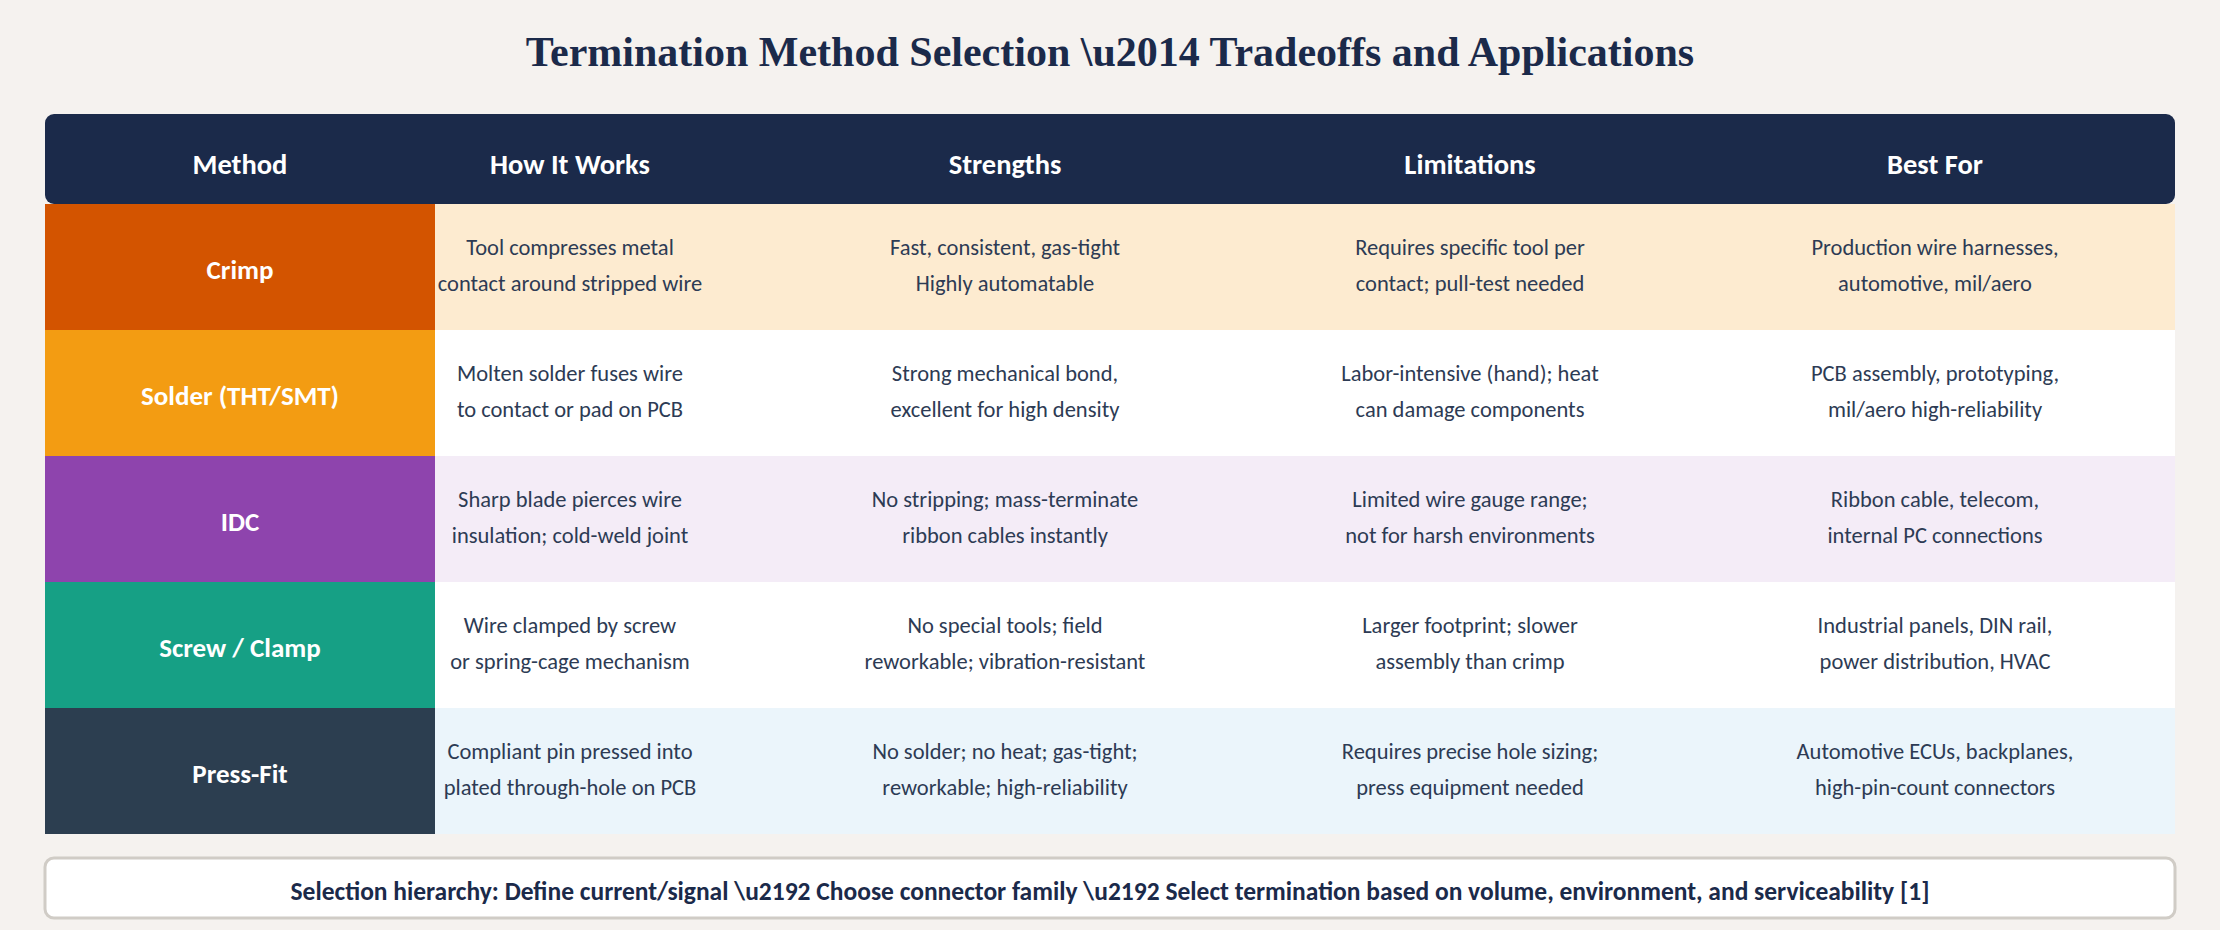
\includegraphics[width=\textwidth]{Electrical and Fluid Connectors/fig2_termination_matrix.png}
\caption{Termination tradeoff matrix --- mechanism, strengths, limitations, and best applications~[1],~[2].}
\label{fig:termination_matrix}
\end{figure}


\subsection{Key Electrical Specifications}
\label{sec:elecspecs}

When specifying an electrical connector in your design documentation, you must define each of the following parameters.

\subsubsection{Current Rating}

The maximum continuous current per contact, in amperes. This depends on contact size, material, plating type, and number of loaded contacts. 

\needspace{4\baselineskip}
\begin{warningbox}[Thermal Derating]
Always derate for multi-pin loaded connectors. When adjacent contacts all carry current, thermal stacking raises the temperature inside the housing, reducing each contact's effective capacity. A connector rated at 10\,A per contact at 25\,\degC may only safely handle 7\,A per contact at 85\,\degC ambient. Manufacturers provide derating curves; never ignore them.
\end{warningbox}

\needspace{4\baselineskip}
\begin{tipbox}[Bridging to Wire Selection (AWG)]
The connector's current rating sets the \emph{minimum} wire gauge you can use. Standard practice: select wire whose ampacity (per NEC Table~310.16 or MIL-W-22759 for aerospace) meets or exceeds the derated connector contact rating. Common reference points for chassis wiring in free air at 30\,\degC: 22~AWG $\approx$ 7\,A, 18~AWG $\approx$ 10\,A, 16~AWG $\approx$ 13\,A, 14~AWG $\approx$ 17\,A, 12~AWG $\approx$ 23\,A, 10~AWG $\approx$ 33\,A. Always verify that the connector contact accepts your chosen wire gauge --- crimp contacts are rated for a specific AWG range (e.g., 18--22~AWG), and using the wrong gauge produces unreliable crimps.
\end{tipbox}

\subsubsection{Voltage Rating}

The maximum working voltage (VAC or VDC). This is determined by creepage (surface distance) and clearance (air gap) distances between adjacent contacts, as specified by IEC~61984~[2]. 

\textbf{Important}: Always specify the \emph{rated working voltage}, not the dielectric withstand (breakdown) voltage. Working voltage includes safety margin; breakdown voltage does not.

\subsubsection{Contact Resistance}

The electrical resistance measured across a mated contact pair, typically in milliohms (\si{\milli\ohm}). Gold-plated contacts achieve $<20\,\mohm$; tin-plated contacts may range from \SIrange{20}{50}{\milli\ohm} when new.

\textbf{Why it matters}: At 10\,A, even $50\mohm$ of contact resistance produces:
\begin{equation}
  P = I^2 R = (10)^2 \times 0.050 = 0.5\,\text{W} \text{ of heat per contact}
\end{equation}
Contact resistance increases with mating cycles and in corrosive environments. Always verify with a milliohm meter during commissioning.

\subsubsection{IP Rating (Ingress Protection)}

Defined by IEC~60529~[3], the IP code uses two digits:
\begin{itemize}[nosep,leftmargin=1.5em]
  \item \textbf{First digit (0--6)}: Protection against solid objects, from ``no protection'' (0) to ``dust-tight'' (6).
  \item \textbf{Second digit (0--9K)}: Protection against liquids, from ``no protection'' (0) to ``high-pressure, high-temperature washdown'' (9K).
\end{itemize}

\begin{table}[ht!]
\centering
\small
\begin{tabular}{c l l}
  \toprule
  \textbf{IP Rating} & \textbf{Meaning} & \textbf{Typical Application} \\
  \midrule
  IP20 & Finger-safe; no liquid protection & Indoor panel wiring \\
  IP54 & Dust-protected; splash-proof & General industrial \\
  IP67 & Dust-tight; 1\,m immersion for 30\,min & Outdoor, vehicle, marine \\
  IP68 & Dust-tight; continuous submersion & Submersible equipment \\
  IP69K & Dust-tight; high-pressure washdown & Food/pharma equipment \\
  \bottomrule
\end{tabular}
\caption{Common IP ratings and their applications.}
\end{table}

\subsubsection{Mating Cycles}

The rated number of connect/disconnect operations before mechanical or electrical degradation. Ranges vary enormously:
\begin{itemize}[nosep,leftmargin=1.5em]
  \item 25--50 cycles: permanent/semi-permanent installations.
  \item 500--1,000 cycles: periodic maintenance access.
  \item 5,000--10,000+ cycles: test fixtures, instrumentation.
\end{itemize}
Gold plating significantly outlasts tin plating. Contact wear directly increases resistance over mating life.


\subsection{Electrical Connector Failure Modes}
\label{sec:elecfailure}

Understanding failure modes is essential for designing robust connections. These are listed roughly in order of how commonly they cause problems in practice.

\subsubsection{Fretting Corrosion}

\textbf{Mechanism}: Micro-motion from vibration (amplitudes as small as 10\,$\mu$m) wears through the contact plating, exposing base metal. Oxides form on the exposed metal, creating high-resistance debris particles that accumulate at the contact interface.

\textbf{Why it's dangerous}: Fretting corrosion is the most insidious failure mode because it develops slowly, manifests as intermittent contact, and is difficult to diagnose. Resistance may fluctuate between normal and open-circuit depending on vibration state.

\textbf{Mitigations}:
\begin{itemize}[nosep,leftmargin=1.5em]
  \item Gold plating (resists oxide formation).
  \item Higher contact normal force (resists micro-motion).
  \item Strain-relief on cables (reduces transmitted vibration).
  \item Secondary locking features on connectors.
\end{itemize}

\begin{figure}[ht!]
\centering
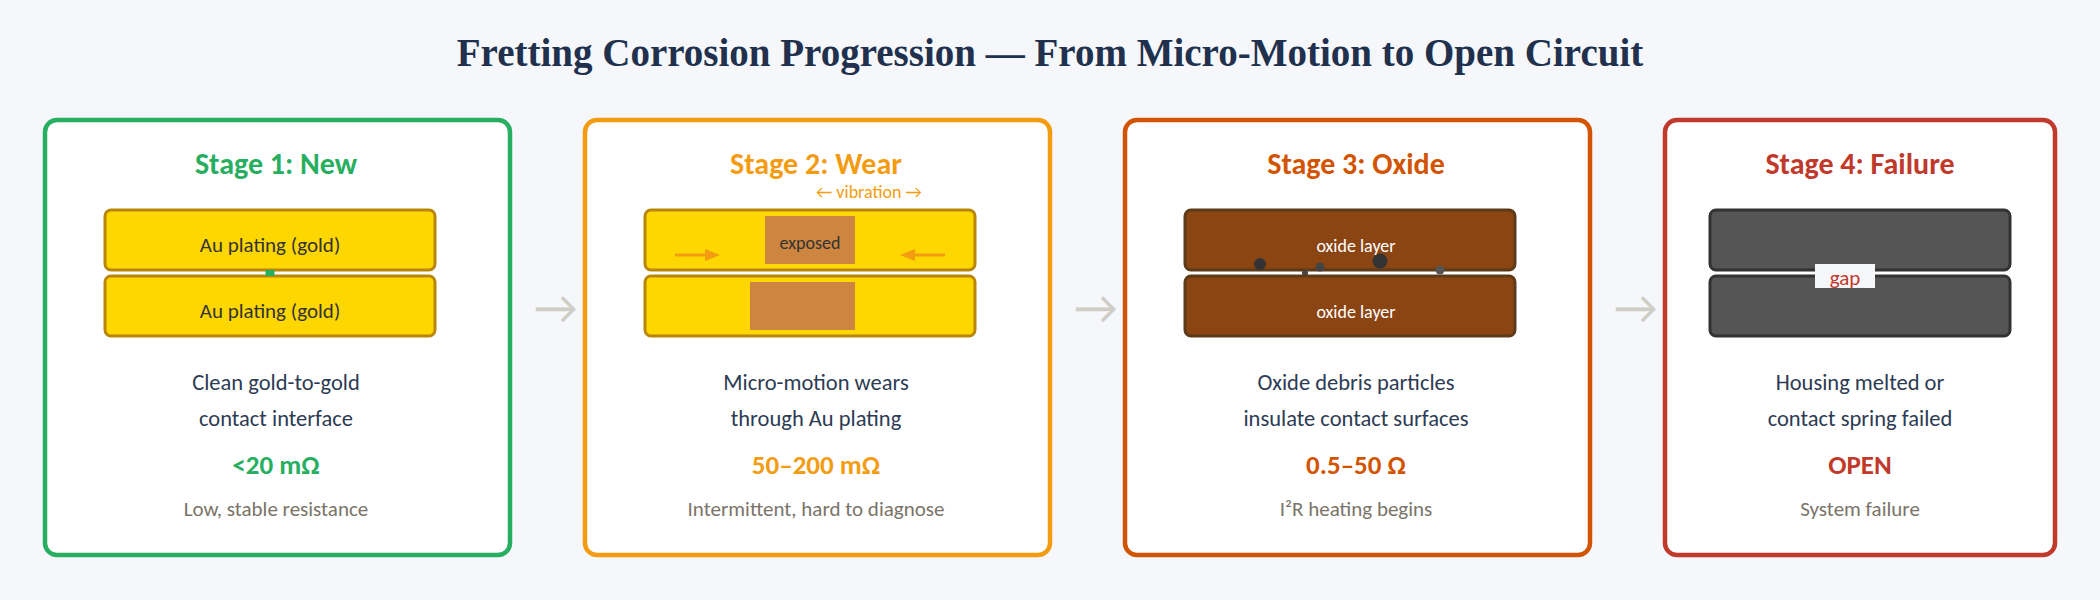
\includegraphics[width=\textwidth]{Electrical and Fluid Connectors/fig7_fretting_progression.png}
\caption{Fretting corrosion progression --- from clean gold-plated contacts through oxide accumulation to open-circuit failure. Note resistance escalation across stages.}
\label{fig:fretting_progression}
\end{figure}

Figure~\ref{fig:fretting_progression} illustrates the four-stage progression of fretting corrosion.  At Stage~1, clean gold-plated contacts exhibit stable resistance below $20\mohm$. Vibration-induced micro-motion gradually wears through the plating at Stage~2, intermittently exposing base metal and raising resistance to \SIrange{50}{200}{\milli\ohm} --- often misdiagnosed as a ``loose connection.'' By Stage~3, accumulated oxide debris insulates the contact surfaces, resistance climbs to the ohm range, and $I^2R$ heating accelerates further degradation. Stage~4 is outright failure: melted housing, collapsed contact springs, or open circuit. Because Stage~2 symptoms are intermittent and position-dependent, fretting often passes bench-top continuity checks only to fail under dynamic load --- a pattern students must learn to recognize.

\subsubsection{Overheating ($I^2 R$ Heating)}

\textbf{Mechanism}: Exceeding the current rating causes resistive heating at the contact interface. Heat accumulates in the housing, softening thermoplastic materials and potentially igniting adjacent insulation or components.

\textbf{Mitigations}:
\begin{itemize}[nosep,leftmargin=1.5em]
  \item Never exceed rated current --- derate for ambient temperature.
  \item Select contacts with lower resistance (gold plating, larger cross-section).
  \item Distribute high currents across multiple contacts.
\end{itemize}

\subsubsection{Creep and Stress Relaxation}

\textbf{Mechanism}: Contact springs gradually lose their clamping force at elevated temperatures. The contact normal force decreases over time, increasing resistance and accelerating other failure modes.

\textbf{Mitigations}:
\begin{itemize}[nosep,leftmargin=1.5em]
  \item Specify beryllium copper (BeCu) contacts for any application above 60\,\degC continuous. BeCu resists creep far better than brass or phosphor bronze.
  \item Overspecify contact normal force for high-temperature applications.
\end{itemize}

\subsubsection{Moisture Ingress}

\textbf{Mechanism}: Water bridges between contacts, causing electrochemical corrosion, increased resistance, or direct short circuits.

\textbf{Mitigations}:
\begin{itemize}[nosep,leftmargin=1.5em]
  \item Specify appropriate IP rating per IEC~60529~[3].
  \item Use sealed connectors with O-ring face seals and wire seals for any outdoor, vehicle, or washdown application.
  \item Apply conformal coating on exposed PCB connections.
\end{itemize}


% ══════════════════════════════════════════════════════════════════════
\FloatBarrier
\section{Fluid System Connectors}
% ══════════════════════════════════════════════════════════════════════

\subsection{Threaded Pipe Fitting Standards}

Two incompatible tapered thread standards dominate global pipe fitting. Geography determines which you encounter.

\subsubsection{NPT --- National Pipe Taper (ASME B1.20.1)}

\begin{itemize}[leftmargin=1.5em]
  \item \textbf{Thread angle}: \ang{60} with pointed crests and roots.
  \item \textbf{Taper}: 1:16 (\textonequarter\,inch per inch of thread length, equivalent to \textthreequarters\,inch per foot).
  \item \textbf{Sealing mechanism}: Thread interference creates a metal-to-metal wedge seal. Because the thread form has clearance at crests and roots, NPT joints \emph{always} require supplemental sealing --- either PTFE (Teflon) tape or anaerobic pipe dope.
  \item \textbf{NPTF variant}: ``Dryseal'' NPT uses a modified thread form with tighter root/crest tolerances that crushes metal at the interface, theoretically sealing without sealant. In practice, sealant is still recommended.
  \item \textbf{Size range}: 1/8\,in.\ to 24\,in.\ nominal pipe size (NPS).
  \item \textbf{Pressure rating}: Up to 15000\,psi depending on material and size.
  \item \textbf{Geography}: Dominant in the United States and Canada.
\end{itemize}

\subsubsection{BSP --- British Standard Pipe (ISO 228 / ISO 7-1)}

\begin{itemize}[leftmargin=1.5em]
  \item \textbf{Thread angle}: \ang{55} Whitworth form with rounded crests and roots.
  \item \textbf{Two sub-types}:
  \begin{itemize}[nosep]
    \item \textbf{BSPT} (designation ``R''): Tapered threads, seals like NPT via thread interference plus sealant.
    \item \textbf{BSPP} (designation ``G''): Parallel (straight) threads that \emph{do not} seal on the threads. Sealing is achieved with a bonded washer or O-ring compressed against a flat face.
  \end{itemize}
  \item \textbf{Size range}: 1/8\,in.\ to 6\,in.\ (inch-denominated but used globally outside North America).
  \item \textbf{Pressure rating}: Up to 6000\,psi typical.
  \item \textbf{Geography}: Dominant in Europe, Asia, and most of the world outside North America.
\end{itemize}

\needspace{4\baselineskip}
\begin{warningbox}[Critical Incompatibility]
NPT (\ang{60} pointed threads) and BSP (\ang{55} rounded threads) are \textbf{NOT} interchangeable. They may appear to engage for a few turns but will not seal properly. Cross-threading causes galling, thread damage, and leaks that may develop catastrophically under pressure. \textbf{Always} verify thread standard with a thread pitch gauge before assembly.
\end{warningbox}

\begin{table}[ht!]
\centering
\small
\begin{tabularx}{\textwidth}{l X X}
  \toprule
  \textbf{Feature} & \textbf{NPT (ASME B1.20.1)} & \textbf{BSP (ISO 228 / ISO 7-1)} \\
  \midrule
  Thread angle & \ang{60}, pointed crests/roots & \ang{55} Whitworth, rounded crests/roots \\
  Taper & 1:16 (all NPT tapered) & BSPT tapered; BSPP parallel \\
  Sealing & Thread interference + sealant & BSPT: thread + sealant; BSPP: washer/O-ring \\
  Geography & U.S., Canada & Europe, Asia, rest of world \\
  Max pressure & 15000\,psi & 6000\,psi typical \\
  \bottomrule
\end{tabularx}
\caption{NPT vs.\ BSP thread comparison.}
\end{table}

\begin{figure}[ht!]
\centering
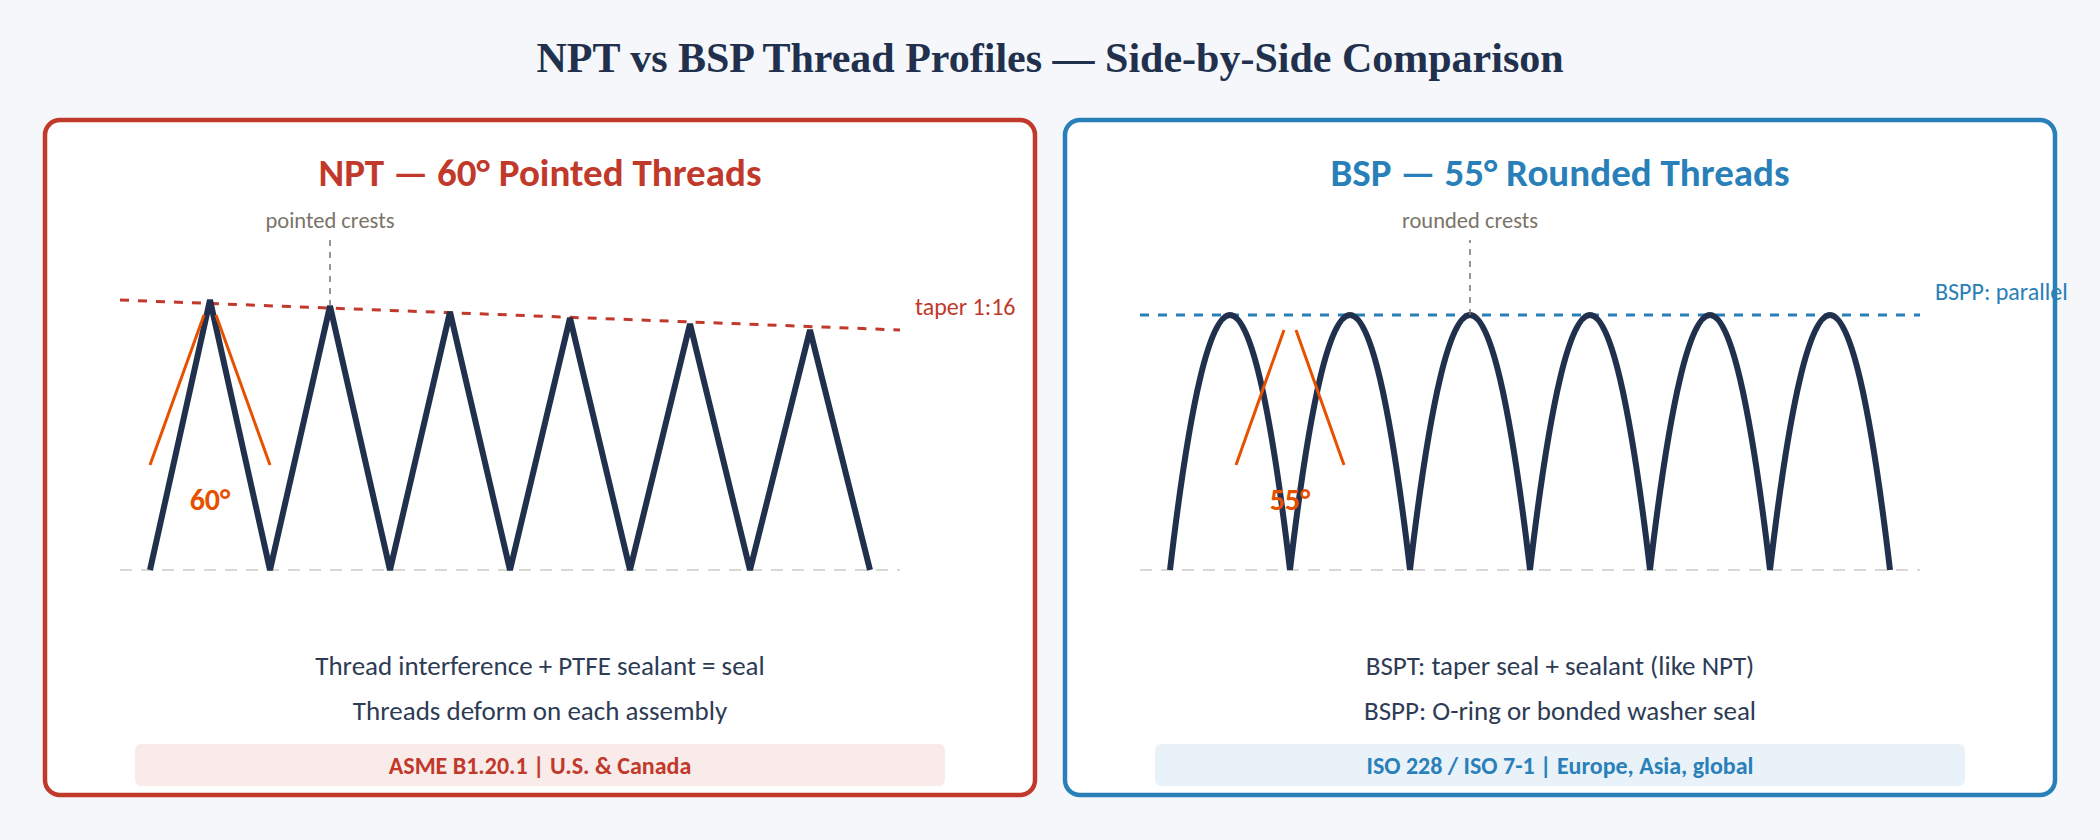
\includegraphics[width=\textwidth]{Electrical and Fluid Connectors/fig5_thread_profiles.png}
\caption{NPT vs.\ BSP thread profiles --- note the pointed \ang{60} crests on NPT versus the rounded \ang{55} Whitworth crests on BSP. These subtle geometric differences make the two standards completely incompatible.}
\label{fig:thread_profiles}
\end{figure}

Figure~\ref{fig:thread_profiles} places the two thread forms side by side so the geometric distinction is immediately visible. NPT's \ang{60} pointed crests create a wedging action as the taper engages --- metal deforms at each assembly, which is why PTFE sealant is required and why each reassembly cycle slightly degrades the thread. BSP's \ang{55} Whitworth form uses rounded crests that are less prone to galling but follow an entirely different pitch schedule. The BSPP (parallel) variant does not seal on the thread at all; the thread merely provides clamping force while an O-ring or bonded washer creates the pressure boundary against a flat face. This is a critical distinction: applying PTFE tape to a BSPP fitting is a common student mistake that serves no purpose and can actually prevent proper washer compression.


\subsection{Tube Fittings and Quick-Connect Couplings}

Unlike threaded pipe fittings (which connect pipes), tube fittings connect \emph{tubing} --- a product specified by outside diameter (OD) and wall thickness, with tighter dimensional tolerances than pipe.

\subsubsection{JIC 37$^{\circ}$\ Flare (SAE J514)}

The tube end is flared to a \ang{37} cone that mates with a matching seat in the fitting body. The joint seals metal-to-metal --- no sealant, tape, or elastomeric seal is required. The fitting uses a straight (non-tapered) thread; the thread provides clamping force only and does not contribute to sealing.

\begin{itemize}[nosep,leftmargin=1.5em]
  \item Reassemblable without degradation (unlike taper threads which deform with each assembly).
  \item The hydraulic industry standard worldwide.
  \item Pressure ratings to 10000\,psi.
  \item AN (Army--Navy) fittings are the military equivalent of JIC, with identical \ang{37} geometry.
\end{itemize}

\subsubsection{Compression Fittings (Swagelok-type)}

One or two ferrules (metal rings) are swaged (compressed) onto the tube OD when the nut is tightened. The ferrule bites into the tube, creating both a grip and a seal.

\begin{itemize}[nosep,leftmargin=1.5em]
  \item No welding, brazing, flaring, or special tools required.
  \item Tube OD is the sizing basis (1/4\,in., 3/8\,in., 1/2\,in., etc.).
  \item \textbf{Gaugeable}: Many designs include a visual indicator (gap gauge) so you can verify proper assembly by inspection.
  \item Pressure ratings up to 20000\,psi for medium-pressure configurations.
  \item Brands: Swagelok, Parker CPI/A-LOK, Ham-Let.
\end{itemize}

\subsubsection{Push-to-Connect}

The tube pushes into the fitting body. An internal collet (toothed ring) grips the tube OD, and an O-ring provides the seal. Assembly is one-handed and tool-free.

\begin{itemize}[nosep,leftmargin=1.5em]
  \item Common in pneumatics (air systems), typically up to $\sim$250\,psi.
  \item Common brands: SMC, Festo, John Guest.
  \item Fast assembly but limited to lower pressures and non-critical sealing applications.
\end{itemize}

\subsubsection{Quick-Disconnect (QD) Couplings}

Two halves --- a plug and a socket --- connect and disconnect by hand, often with a locking sleeve or collar. Self-sealing valves in one or both halves prevent fluid loss on disconnect.

\begin{itemize}[nosep,leftmargin=1.5em]
  \item \textbf{Flat-face}: Minimal fluid spillage on disconnect, used in clean or environmentally sensitive applications.
  \item \textbf{Poppet-valve}: Spring-loaded valve seals on disconnect, less expensive but more spillage.
  \item Common applications: hydraulic tool circuits, coolant loops, test equipment.
\end{itemize}

\begin{table}[ht!]
\centering
\small
\begin{tabularx}{\textwidth}{l c c X}
  \toprule
  \textbf{Fitting Family} & \textbf{Pressure} & \textbf{Seal Type} & \textbf{Key Characteristic} \\
  \midrule
  JIC 37$^{\circ}$\ Flare & 10000\,psi & Metal-to-metal & Reassemblable; hydraulic standard \\
  Compression & 20000\,psi & Ferrule swage & No special tools; gaugeable \\
  Push-to-Connect & 250\,psi & O-ring & Tool-free; pneumatics \\
  Quick-Disconnect & Varies & Valve + O-ring & Hand-connect; self-sealing \\
  \bottomrule
\end{tabularx}
\caption{Tube fitting and coupling comparison.}
\end{table}

\begin{figure}[ht!]
\centering
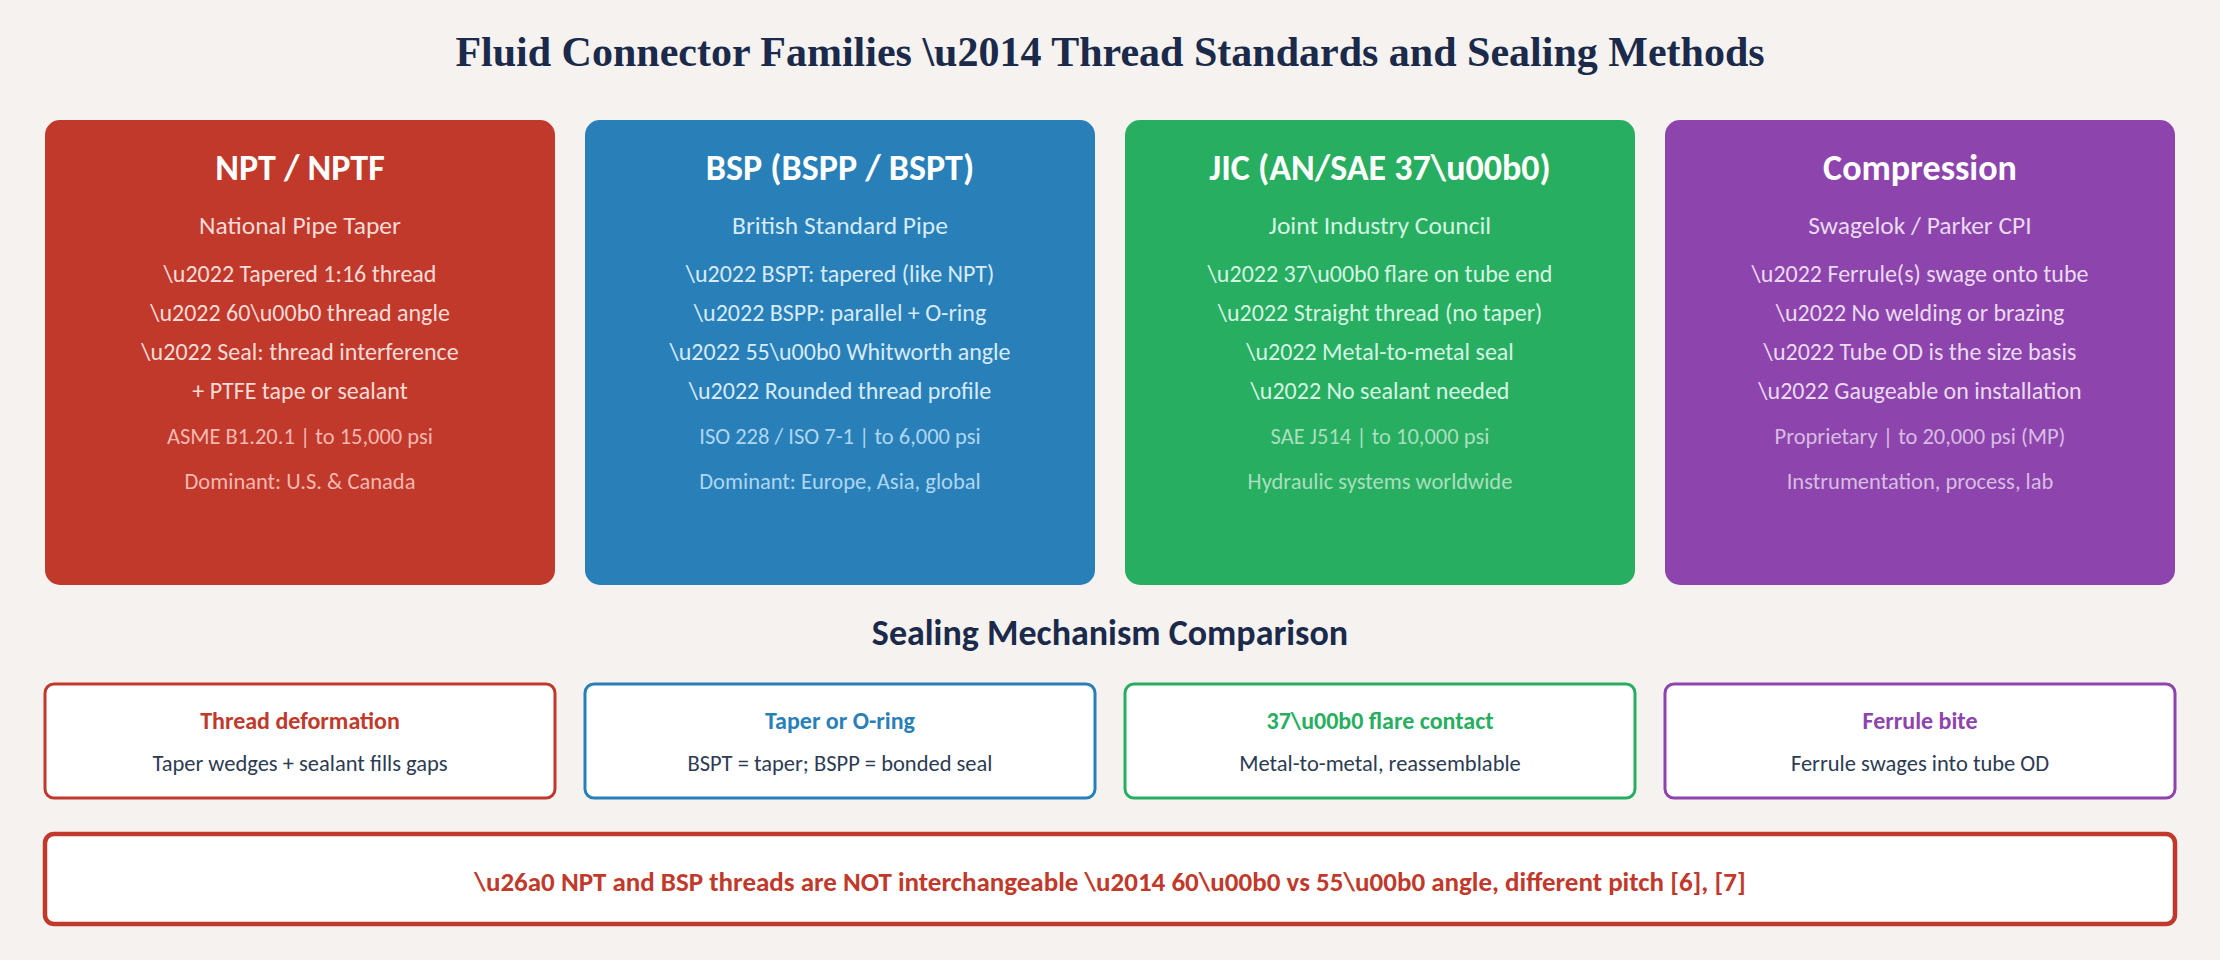
\includegraphics[width=\textwidth]{Electrical and Fluid Connectors/fig3_fluid_connectors.png}
\caption{Four major fluid connector families with thread standards, pressure ratings, and sealing mechanisms.}
\label{fig:fluid_connectors}
\end{figure}

\begin{figure}[ht!]
\centering
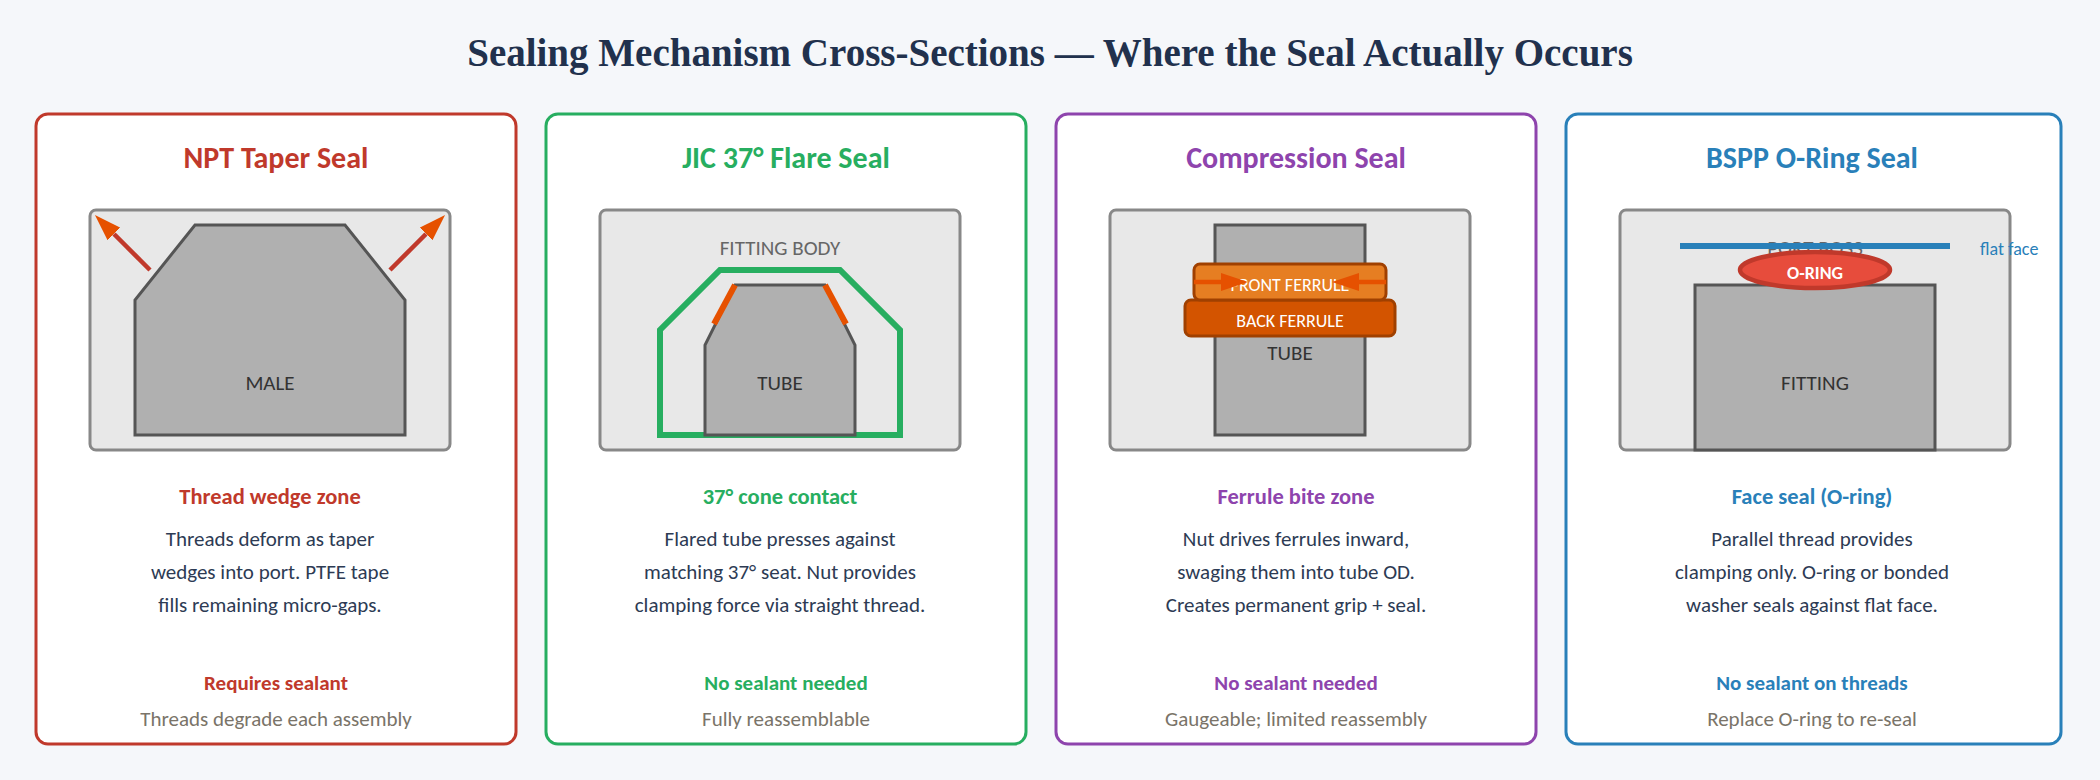
\includegraphics[width=\textwidth]{Electrical and Fluid Connectors/fig6_seal_cross_sections.png}
\caption{Sealing mechanism cross-sections showing exactly where each seal forms: NPT thread wedge, JIC \ang{37} flare cone contact, compression ferrule bite zone, and BSPP face-seal O-ring.}
\label{fig:seal_cross_sections}
\end{figure}

Figure~\ref{fig:seal_cross_sections} shows the internal geometry of each sealing method so students can visualize \emph{why} proper torque and assembly procedures matter. In the NPT taper seal, the thread flanks themselves deform to create a pressure boundary --- which is why sealant is mandatory to fill the remaining micro-gaps and why repeated assembly progressively damages the seal surfaces. In the JIC \ang{37} flare, the cone-shaped tube end presses against a matching seat in the fitting body; the straight thread provides clamping force only. This metal-to-metal geometry is fully reassemblable because the sealing surfaces do not deform. In compression fittings, the front ferrule bites radially into the tube OD while the back ferrule provides axial grip; the nut drives both ferrules during initial makeup. Once swaged, the ferrule is permanently deformed, which limits reassembly. In the BSPP face seal, the parallel thread clamps the fitting against the port face while an O-ring in a groove creates the pressure boundary --- the thread contributes zero sealing.


\subsection{Key Fluid Connector Specifications}
\label{sec:fluidspecs}

When specifying a fluid connector in your design documentation, define each of the following.

\subsubsection{Working Pressure}

The maximum continuous operating pressure (psi or bar). Always specify \emph{working} pressure, not burst pressure. Standard safety factors:
\begin{itemize}[nosep,leftmargin=1.5em]
  \item Hydraulic: burst $\geq 4\times$ working.
  \item Pneumatic: burst $\geq 3\times$ working.
  \item \textbf{Design rule}: Never operate above 25\% of burst pressure.
\end{itemize}

\subsubsection{Temperature Range}

Temperature determines seal material selection:

\begin{table}[ht!]
\centering
\small
\begin{tabularx}{\textwidth}{l c X}
  \toprule
  \textbf{Seal Material} & \textbf{Range} & \textbf{Notes} \\
  \midrule
  Buna-N (Nitrile, NBR) & $-40$ to 250\,$^{\circ}$F & General purpose; petroleum-compatible \\
  Viton (FKM) & $-20$ to 400\,$^{\circ}$F & Chemical resistance; fuel systems \\
  PTFE (Teflon) & $-100$ to 500\,$^{\circ}$F & Widest range; chemically inert; no elasticity \\
  EPDM & $-65$ to 300\,$^{\circ}$F & Steam/water service; not oil-compatible \\
  \bottomrule
\end{tabularx}
\caption{Seal material temperature ranges and applications.}
\end{table}

Always verify seal compatibility with both the fluid \emph{and} the operating temperature.

\subsubsection{Fluid Compatibility}

Verify fitting body material and seal material against the working fluid using manufacturer chemical compatibility charts:
\begin{itemize}[nosep,leftmargin=1.5em]
  \item \textbf{Stainless steel}: Resists most chemicals; highest cost.
  \item \textbf{Brass}: Common for water, air, and general service; not for ammonia or acetylene.
  \item \textbf{Carbon steel}: Standard for hydraulic oil systems; requires corrosion protection.
\end{itemize}

\subsubsection{Thread / Tube Size}

\begin{itemize}[nosep,leftmargin=1.5em]
  \item \textbf{Threaded fittings}: Specified by Nominal Pipe Size (NPS). Note that NPS does \emph{not} equal the actual outside diameter. For example, 1/2\,in.\ NPS pipe has an OD of 0.840\,in.
  \item \textbf{Tube fittings}: Specified by tube outside diameter (OD). Common sizes: 1/4\,in., 3/8\,in., 1/2\,in.
  \item \textbf{Always measure with calipers and thread gauges} --- never assume a size by visual inspection.
\end{itemize}

\subsubsection{End Configuration}

Select the geometry that connects the fitting to your system: straight, elbow (45$^{\circ}$\ or 90$^{\circ}$), tee, cross, union, reducer, or bulkhead. 

\needspace{4\baselineskip}
\begin{tipbox}[Minimize Joints]
Every fitting joint is a potential leak point. Design your routing to minimize the total number of fittings in a line. Avoid stacking street elbows in series --- use a single 90$^{\circ}$\ elbow or a pre-bent tube run instead.
\end{tipbox}


\subsection{Fluid Connector Failure Modes}
\label{sec:fluidfailure}

\subsubsection{Cross-Threading}

\textbf{Mechanism}: Attempting to mate NPT into BSP (or vice versa) --- or even same-standard threads started at an angle --- destroys thread profiles and causes immediate or delayed leaks.

\textbf{Mitigations}:
\begin{itemize}[nosep,leftmargin=1.5em]
  \item Always verify thread standard with a thread pitch gauge before assembly.
  \item Start threads by hand for at least two full turns before applying a wrench.
  \item NPT: \ang{60} pointed threads. BSP: \ang{55} rounded threads. They \emph{feel} similar but are not compatible.
\end{itemize}

\subsubsection{Over-Tightening}

\textbf{Mechanism}: Excessive torque cracks port bosses (especially aluminum and cast iron), deforms compression ferrules beyond recovery, and splits flare cones. Over-tightening destroys more fittings than under-tightening.

\textbf{Mitigations}:
\begin{itemize}[nosep,leftmargin=1.5em]
  \item Always use manufacturer-specified torque values.
  \item Use a calibrated torque wrench, not a ``feel'' wrench.
  \item For Swagelok-type fittings, follow the turns-past-finger-tight specification exactly.
\end{itemize}

\subsubsection{Seal Degradation}

\textbf{Mechanism}: O-rings and gaskets deteriorate from chemical attack (incompatible fluid), UV exposure, thermal cycling, and simple age. Seals swell, harden, crack, or take a permanent compression set.

\textbf{Mitigations}:
\begin{itemize}[nosep,leftmargin=1.5em]
  \item Establish replacement intervals based on seal material and service conditions.
  \item Keep spare seal kits on hand.
  \item Verify seal material compatibility with the fluid and temperature range before installation.
\end{itemize}

\subsubsection{Vibration Fatigue}

\textbf{Mechanism}: Cyclic stress at tube-to-fitting junctions nucleates fatigue cracks. Under pressure, these cracks propagate to failure --- potentially a sudden, high-pressure fluid release.

\textbf{Mitigations}:
\begin{itemize}[nosep,leftmargin=1.5em]
  \item Use proper tube support clamps spaced per manufacturer recommendations.
  \item Route tubing to avoid sharp bends and unsupported cantilever lengths.
  \item Include flexible hose segments at vibration sources (pumps, engines).
\end{itemize}

\needspace{4\baselineskip}
\begin{warningbox}[High-Pressure Fluid Injection Injury]
A hydraulic line leak may be invisible --- a pinhole stream at 2000\,psi can penetrate skin and inject fluid deep into tissue, causing catastrophic damage that requires emergency surgery within hours. \textbf{Never} check for hydraulic leaks by running a bare hand along a pressurized line. Use a piece of cardboard or a thermal camera instead. This is one of the most serious and least-understood hazards in hydraulic system work, and students designing or testing any pressurized fluid system must be explicitly aware of it before commissioning.
\end{warningbox}


% ══════════════════════════════════════════════════════════════════════
\FloatBarrier
\section{Selection and Design Practice}
% ══════════════════════════════════════════════════════════════════════

\subsection{Connector Selection Logic}

Whether electrical or fluid, connector selection follows a universal logic sequence:

\begin{enumerate}[leftmargin=1.5em]
  \item \textbf{Rating}: What current, voltage, pressure, or flow must it handle?
  \item \textbf{Environment}: Temperature range, vibration, moisture/IP, chemical exposure?
  \item \textbf{Serviceability}: How often must it be connected/disconnected? What tools are available?
  \item \textbf{Cost}: What is the budget per connection, including tooling?
  \item \textbf{Standards}: Which industry/regulatory standards apply (IEC, SAE, ASME, MIL)?
  \item \textbf{Space}: What are the physical envelope constraints?
\end{enumerate}

\begin{figure}[ht!]
\centering
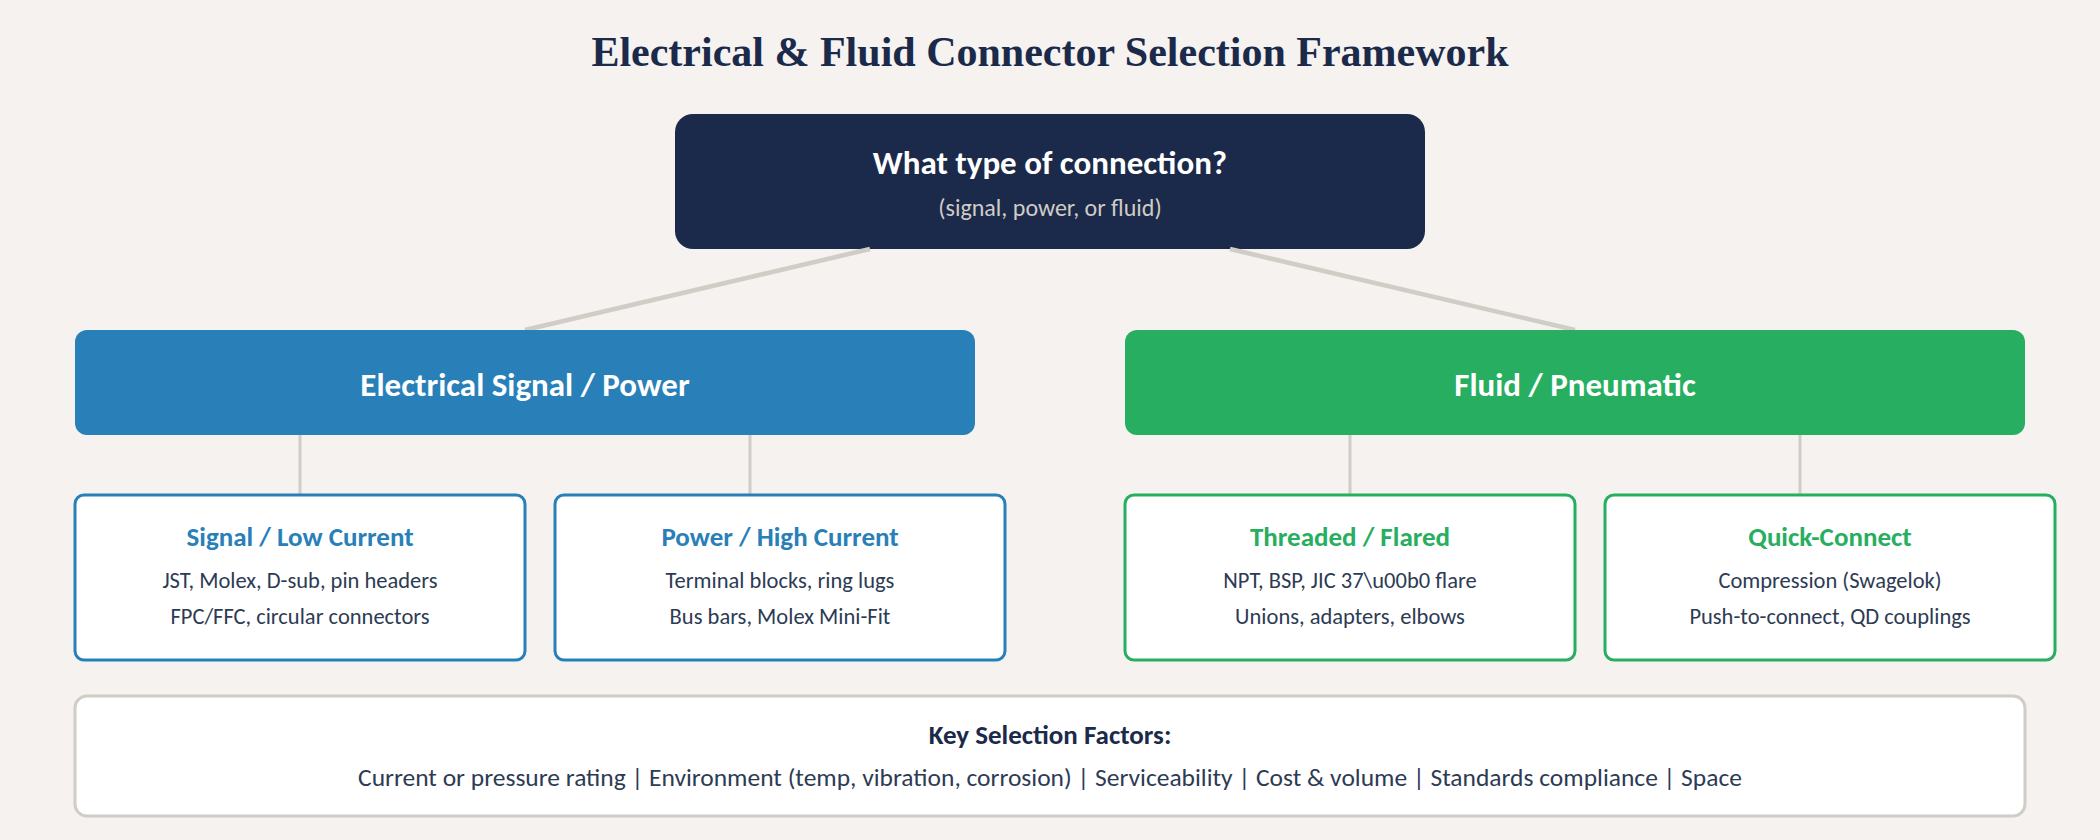
\includegraphics[width=\textwidth]{Electrical and Fluid Connectors/fig4_selection_framework.png}
\caption{Decision tree for electrical and fluid connector selection.}
\label{fig:selection_framework}
\end{figure}

\needspace{4\baselineskip}
\begin{tipbox}[Spec the Connector First]
The connector determines wire gauge, tube OD, termination tooling, and housing envelope. Select the connector family first (based on rating, environment, and serviceability), then design the wiring or tubing around it --- not the other way around.
\end{tipbox}

\subsection{Design Rules of Thumb}

\begin{enumerate}[leftmargin=1.5em]
  \item \textbf{Derate everything.} Never operate at 100\% of rated current, pressure, or temperature. A 25\% safety margin is minimum engineering practice; 50\% is professional practice for critical systems.

  \item \textbf{Design for Assembly (DFA).} Provide wrench clearance around fittings. Group fluid connections for leak-test access. Use consistent connector families within a subsystem to reduce tool count and spare parts inventory.

  \item \textbf{For fluid systems}: Verify thread standard with a gauge before assembly. Use manufacturer torque specifications. Pressure-test every joint before commissioning --- hydrostatic test at $1.5\times$ working pressure per ASME B31.3~[8].

  \item \textbf{For electrical systems}: Pull-test a sample of crimps per IPC/WHMA-A-620. Verify contact resistance with a milliohm meter. Document every connector in your wire harness schedule.

  \item \textbf{Document every choice.} Record part number, manufacturer, specifications, and selection rationale in your Bill of Materials (BOM). Your future self and your teammates will need this information for procurement, assembly, and troubleshooting.
\end{enumerate}


\subsection{Key Standards Reference}

\begin{longtable}{l l p{7.5cm}}
  \toprule
  \textbf{Standard} & \textbf{Org} & \textbf{Scope} \\
  \midrule
  \endfirsthead
  \toprule
  \textbf{Standard} & \textbf{Org} & \textbf{Scope} \\
  \midrule
  \endhead
  IEC 61984~[2] & IEC & Electrical connector safety requirements, testing, and performance criteria \\
  IEC 60529~[3] & IEC & IP ingress protection rating system (IP67, IP68, IP69K) \\
  MIL-DTL-38999~[4] & U.S.\ DoD & Military circular connectors for high-performance, harsh-environment applications \\
  UL 486A-486B & UL & Safety certification for wire connectors: crimp, solder, and IDC terminations \\
  SAE J514~[5] & SAE & JIC 37$^{\circ}$\ flare hydraulic tube fittings --- dimensions and performance requirements \\
  ASME B1.20.1~[6] & ASME & NPT tapered pipe thread form, dimensions, and tolerances \\
  ISO 228 / ISO 7-1~[7] & ISO & BSP parallel (BSPP) and tapered (BSPT) pipe thread standards \\
  ASME B31.3~[8] & ASME & Process piping code --- materials, fabrication, inspection, and testing \\
  \bottomrule
\end{longtable}


% ══════════════════════════════════════════════════════════════════════
\FloatBarrier
\section{Applying Connectors in Your Design Projects}
% ══════════════════════════════════════════════════════════════════════

Incorrect connector selection is one of the most common failure modes in student design projects. The following workflow ensures systematic coverage.

\begin{enumerate}[leftmargin=1.5em]
  \item \textbf{Create a connection schedule early.} List every electrical and fluid joint in your design. Classify each by type (wire-to-wire, wire-to-board, NPT, JIC, etc.). This becomes a living document through your design reviews.

  \item \textbf{For every electrical connection, specify}: connector family, pin count, current rating (derated), voltage rating, IP rating, termination method, wire gauge, and mating cycles.

  \item \textbf{For every fluid connection, specify}: fitting standard (NPT, BSP, JIC, or compression), nominal size, working pressure, seal material, fluid compatibility, and assembly torque.

  \item \textbf{Build a complete BOM} with manufacturer part numbers and procurement sources. Recommended suppliers:
  \begin{itemize}[nosep]
    \item Electrical: Digi-Key, Mouser, Newark, Allied.
    \item Fluid: Swagelok, Parker, McMaster-Carr, Grainger.
  \end{itemize}

  \item \textbf{Design review milestones}:
  \begin{itemize}[nosep]
    \item \textbf{PDR}: Present your connection schedule.
    \item \textbf{CDR}: Present datasheets and torque specifications.
    \item \textbf{FDR}: Demonstrate assembly procedures and test results.
  \end{itemize}

  \item \textbf{Test every connection before commissioning}: Pull-test electrical crimps, measure contact resistance with a milliohm meter, and pressure-test all fluid joints at $1.5\times$ working pressure.
\end{enumerate}


% ══════════════════════════════════════════════════════════════════════
\FloatBarrier
\section{Quick-Reference Summary}
% ══════════════════════════════════════════════════════════════════════

\needspace{4\baselineskip}
\begin{keyconceptbox}[Five Key Takeaways]
\begin{enumerate}[nosep,leftmargin=1.5em]
  \item Electrical connectors are classified by \emph{what they connect} (wire-to-wire, wire-to-board, board-to-board) and \emph{how they terminate} (crimp, solder, IDC, screw, press-fit).
  \item For every electrical connection, specify: current rating, voltage rating, IP rating, contact resistance, and mating cycles --- and derate for temperature.
  \item Fluid connectors require matching thread standards --- NPT $\neq$ BSP. JIC 37$^{\circ}$\ flare and compression fittings avoid the pitfalls of tapered-thread sealing.
  \item Failure modes differ by domain: electrical joints fail from fretting corrosion and $I^2R$ overheating; fluid joints fail from cross-threading and seal degradation.
  \item Every connector specification follows the same logic: \textbf{rating $\to$ environment $\to$ serviceability $\to$ cost $\to$ standards $\to$ space}. Document everything in your BOM.
\end{enumerate}
\end{keyconceptbox}


% ══════════════════════════════════════════════════════════════════════
\FloatBarrier
\section{Practice Questions for Quiz Preparation}
% ══════════════════════════════════════════════════════════════════════

Use these questions to test your understanding. Answers follow on the next page.

\subsection{Conceptual Questions}

\begin{enumerate}[leftmargin=1.5em]
  \item What are the three fundamental elements of every electrical connector?

  \item A connector is rated at 15\,A per contact at 25\,\degC. Your design has an ambient temperature of 75\,\degC and all 12 contacts are loaded. Why should you \emph{not} assume 15\,A per contact is safe?

  \item Explain why fretting corrosion is considered the ``most insidious'' electrical connector failure mode.

  \item You need to connect a hydraulic line rated at 5000\,psi that will be disconnected for maintenance monthly. Which fitting family is most appropriate? Why?

  \item A colleague suggests using PTFE tape on a BSPP fitting. Is this correct? Explain.

  \item What is the difference between rated working voltage and dielectric withstand voltage? Which should appear in your design documentation?

  \item Why does NPS (Nominal Pipe Size) create confusion when specifying fittings?

  \item Describe two mitigations for vibration fatigue in fluid tubing systems.

  \item You measure $50\mohm$ contact resistance on a connector carrying 8\,A. How much power is dissipated as heat at that contact? Is this a concern?

  \item Compare the sealing mechanisms of NPT, JIC 37$^{\circ}$\ flare, and compression fittings. Which requires sealant?
\end{enumerate}

\subsection{Application / Scenario Questions}

\begin{enumerate}[resume,leftmargin=1.5em]
  \item Your design team is designing an outdoor weather station. You need a 6-pin connector for sensor signals (all under 500\,mA) that will be installed once and never disconnected. What IP rating, plating, and mating-cycle specification would you select? Justify your choices.

  \item A pneumatic system in your project uses 1/4\,in.\ OD nylon tubing at 80\,psi. Recommend a fitting type and explain why.

  \item Your design uses both NPT and BSP components (sourced from U.S.\ and European manufacturers). What steps must you take to ensure safe assembly?

  \item You are specifying connectors for a cooling loop carrying a 50/50 ethylene glycol--water mix at 200\,$^{\circ}$F and 50\,psi. What seal material would you select? What body material?

  \item At your CDR, a reviewer asks: ``How did you verify your crimp terminations are reliable?'' Describe the test procedure you would reference.

  \item \textbf{Diagnostic scenario}: Your team's prototype passes a low-voltage continuity check on the bench (all connections show $<1\,\Omega$), but the system experiences intermittent sensor dropouts and a motor controller that occasionally faults when the prototype is running on a vibration table or driving over rough terrain. Where do you start your investigation, and what failure modes should you suspect? Describe the diagnostic steps you would take, referencing at least three concepts from this module.
\end{enumerate}


\newpage
\subsection{Answers}

\begin{enumerate}[leftmargin=1.5em]
  \item Contacts (conductive pins/sockets), housing (insulating body), and termination (wire-to-contact joint).

  \item Two derating effects compound: (a) elevated ambient temperature reduces the thermal headroom of the housing, and (b) thermal stacking from all 12 contacts being loaded raises the internal housing temperature further. The manufacturer's derating curve must be consulted; actual safe current per contact could be as low as 10\,A or less.

  \item Fretting corrosion develops slowly from micro-vibration, manifests as intermittent (not permanent) high resistance, is invisible without disassembly, and is difficult to reproduce during troubleshooting. By the time symptoms are consistent, oxide debris has accumulated extensively.

  \item JIC 37$^{\circ}$\ flare (SAE J514). It handles 10000\,psi (well above 5000\,psi), provides a metal-to-metal seal that doesn't degrade with reassembly, and is designed for repeated disconnect/reconnect without special tools beyond standard wrenches. Compression would also work but ferrules deform on initial assembly, making reassembly less reliable.

  \item Incorrect. BSPP (G-type) uses parallel threads that do \emph{not} seal on the threads. Sealing is achieved with a bonded washer or O-ring against a flat face. PTFE tape is used on \emph{tapered} threads (NPT, BSPT) where the thread interference provides the primary seal. Applying tape to BSPP serves no useful purpose and may prevent proper washer compression.

  \item Working voltage is the maximum voltage at which the connector is rated for continuous, safe operation, including creepage and clearance margins per IEC 61984. Dielectric withstand (breakdown) voltage is the voltage at which insulation fails --- it is a destructive test limit, not an operating specification. Always specify working voltage in design documentation.

  \item NPS is a nominal designation, not a physical dimension. For example, 1/2\,in.\ NPS has an OD of 0.840\,in. Engineers unfamiliar with this convention may attempt to match fittings by measuring OD, leading to incorrect specifications. Always reference the NPS table and verify with thread gauges.

  \item (a) Install tube support clamps at manufacturer-recommended intervals to eliminate unsupported spans. (b) Include flexible hose segments at vibration sources (pumps, engines) to decouple cyclic motion from rigid tubing.

  \item $P = I^2R = (8)^2 \times 0.050 = 3.2\,\text{W}$. Yes, this is a concern --- 3.2\,\text{W} of localized heat will raise the contact and housing temperature significantly. This level of contact resistance suggests degraded contacts that should be inspected and potentially replaced.

  \item NPT: Thread interference creates a wedge seal, but clearance at crests/roots requires supplemental sealant (PTFE tape or pipe dope). JIC 37$^{\circ}$: Metal-to-metal cone seal at the flared tube end; no sealant required. Compression: Ferrule swaged onto tube OD creates the seal mechanically; no sealant required. Only NPT (and BSPT) requires sealant.

  \item IP67 (dust-tight, survives 1\,m immersion for rain/flooding protection). Gold plating (resists corrosion in outdoor environment with humidity and temperature cycling). 25--50 mating cycles (permanent installation, only disconnected for rare maintenance). Lower mating cycle connectors are less expensive and can be more robust.

  \item Push-to-connect fittings. At 80\,psi with nylon tubing, this is well within the 250\,psi range of push-to-connect. Benefits: tool-free assembly, compatible with nylon tubing, easy reconfiguration, and widely available in 1/4\,in.\ OD size from SMC, Festo, or John Guest.

  \item (a) Create a thread identification chart for the project listing which ports are NPT and which are BSP. (b) Verify every connection with a thread pitch gauge (\ang{60} = NPT, \ang{55} = BSP) before assembly. (c) If adaptation is needed, use NPT-to-BSP adapter fittings from a reputable manufacturer --- never force-thread. (d) Label all ports on your assembly drawings with thread standard.

  \item Seal: Viton (FKM) --- compatible with ethylene glycol, rated to 400\,$^{\circ}$F (above the 200\,$^{\circ}$F operating temperature). Body: stainless steel or brass (both compatible with glycol--water). Avoid carbon steel unless corrosion-protected, as glycol solutions can be mildly corrosive to unprotected ferrous metals.

  \item Reference IPC/WHMA-A-620 standard. Procedure: (a) Pull-test a statistical sample of crimps at the specified force for the wire gauge and contact size. (b) Cross-section a sample crimp to verify the cold-weld zone under magnification. (c) Measure contact resistance across each mated pair with a milliohm meter --- verify $<20\,\mohm$ for gold-plated contacts. (d) Document results with crimp force values, pass/fail criteria, and inspector sign-off.

  \item This scenario synthesizes three interconnected failure modes. \textbf{Primary suspect: fretting corrosion.} The hallmark is a system that passes static bench testing but fails under dynamic load --- exactly the intermittent, vibration-dependent behavior described in the fretting progression (Section~\ref{sec:elecfailure}, Figure~\ref{fig:fretting_progression}). Diagnostic steps: (a)~Measure contact resistance across every mated connector pair with a milliohm meter \emph{while the system is subject to vibration} (tap on connectors, flex cables). Resistance that fluctuates from milliohms to ohms on disturbance confirms fretting. (b)~Check for $I^2R$ heating: use a thermal camera to identify hot connectors under load. A connector running 10\,A through a fretting contact at $500\mohm$ dissipates 5\,\text{W} --- enough to soften a nylon housing. (c)~Inspect strain relief: if cables transmit vehicle vibration directly to the contact zone, fretting is accelerated regardless of plating. (d)~Check connector specifications: are tin-plated contacts being used in a high-vibration application where gold plating is warranted? Is the contact normal force sufficient? (e)~For the motor controller faults specifically, consider whether the power connector is derated for the actual ambient temperature inside the enclosure under operation. Resolution: replace affected contacts with gold-plated equivalents, add proper strain-relief clamps, install secondary locking features (CPA clips), and retest under dynamic load with milliohm monitoring.
\end{enumerate}


% ══════════════════════════════════════════════════════════════════════

\FloatBarrier
\chapter{Power Supplies, Motors \& Pumps}

\vspace{1em}




\vspace{1em}

% ══════════════════════════════════════════════════════════════════════
\FloatBarrier
\section{Power Supply Selection}
% ══════════════════════════════════════════════════════════════════════

\subsection{What a Power Supply Does}

A power supply converts electrical energy from a source --- AC mains, battery, solar panel, or USB --- into one or more regulated DC voltage rails that your circuits and actuators require. Every component in your design has a specific voltage and current requirement. A typical student project might need 3.3\,V for the microcontroller, 5\,V for sensors and logic, and 12\,V or 24\,V for motors and solenoids. The power supply must deliver all of these simultaneously with adequate regulation and current capacity.

\subsection{Linear Regulators (LDO)}

Linear regulators are the simplest power supply topology. They are essentially a controllable series resistance that drops the input voltage to the desired output, dissipating the excess as heat.

\begin{equation}
  P_{\text{waste}} = (V_{\text{in}} - V_{\text{out}}) \times I_{\text{load}}, \qquad \eta = \frac{V_{\text{out}}}{V_{\text{in}}} \times 100\%
\end{equation}

An LM7805 producing 5\,V from 12\,V at 1\,A wastes 7\,\text{W} as heat with only 42\% efficiency. A low-dropout (LDO) regulator reduces the minimum input-to-output voltage difference to as little as 200\,mV, improving efficiency when the differential is small.

\needspace{4\baselineskip}
\begin{tipbox}[When to Use an LDO]
Use LDOs when: (1) the voltage drop is small ($<2\,V$), (2) current is under $\sim$1\,A, (3) noise matters (analog sensors, audio, ADCs), or (4) simplicity matters (only 2 capacitors, no inductor needed). Common devices: LM7805 (5\,V/1\,A), AMS1117-3.3 (3.3\,V/1\,A), MCP1700 (3.3\,V/250\,mA, ultra-low quiescent current).
\end{tipbox}

\subsection{Switching Regulators (DC-DC Converters)}

Switching regulators chop the input voltage at high frequency (100\,kHz--2\,MHz) and use an inductor to transfer energy efficiently, achieving 85--95\% efficiency.

\subsubsection{Buck (Step-Down): $V_{\text{out}} < V_{\text{in}}$}

The workhorse of DC-DC conversion. A switching FET, inductor, and capacitor step voltage down. Typical efficiency 85--95\%. Common devices: LM2596 (3\,A), MP1584 (3\,A), TPS54302 (3\,A). Pre-built module boards are available for under \$2 --- recommended for student projects because the critical PCB layout is already done.

\textbf{Example}: 12\,V battery $\to$ 5\,V at 2\,A. At 90\% efficiency, waste heat is only 1.1\,\text{W} compared to 14\,\text{W} for a linear regulator.

\subsubsection{Boost (Step-Up): $V_{\text{out}} > V_{\text{in}}$}

Stores energy in an inductor during the switch-on phase, then releases it at higher voltage during switch-off. Typical efficiency 80--93\%. Common devices: MT3608 (2\,A), TPS61088 (10\,A). Important limitation: most boost converters cannot fully disconnect the load from the input.

\subsubsection{Buck-Boost: $V_{\text{out}} \gtrless V_{\text{in}}$}

Handles input voltage that swings above and below the output --- essential for battery applications. A LiPo cell ranges from 4.2\,V (full) to 3.0\,V (depleted). If your circuit needs 3.3\,V, the input crosses the output during discharge. Only buck-boost works through this transition. Common: TPS63020 (3.6\,A), LTC3780.

\needspace{4\baselineskip}
\begin{warningbox}[EMI from Switching Regulators]
All switching regulators generate electromagnetic interference at their switching frequency. This can corrupt ADC readings, cause radio interference, and inject noise into audio circuits. Always follow the datasheet layout recommendations: keep switching traces short, use a continuous ground plane, and place input/output capacitors as close to the regulator as physically possible. When powering noise-sensitive circuits, add an LDO downstream of the switcher as a noise filter.
\end{warningbox}

\subsection{AC-DC Power Supplies}

For systems that plug into AC mains (120/240\,VAC), you need an AC-to-DC conversion stage with galvanic isolation to separate lethal mains voltage from safe low-voltage outputs.

\needspace{4\baselineskip}
\begin{warningbox}[Student Project Rule]
\textbf{Never design your own AC-DC converter.} Always use a pre-certified wall adapter (UL/CE listed) that provides a regulated DC output. These are fully enclosed, safety-certified, and eliminate all mains-voltage hazards from your design. If a wall adapter cannot meet your requirements, use an enclosed industrial supply (Mean Well, TDK-Lambda) with proper enclosure design.
\end{warningbox}

\subsection{Key Power Supply Specifications}
\label{sec:psu_specs}

\begin{table}[ht!]
\centering\small
\begin{tabularx}{\textwidth}{l X}
  \toprule
  \textbf{Specification} & \textbf{Description} \\
  \midrule
  Output Voltage & Nominal output with tolerance (e.g., 5.0\,V $\pm$2\%). Must match each load rail. \\
  Output Current & Max continuous delivery. Must exceed total load current with $\geq$20\% margin. \\
  Regulation & Line regulation: output change when input varies. Load regulation: output change when load varies. Expressed as \% or mV. \\
  Ripple \& Noise & Peak-to-peak AC on the DC output. Switchers: 20--100\,mV. LDOs: $<$1\,mV. \\
  Efficiency & $P_{\text{out}} / P_{\text{in}} \times 100\%$. LDO: 40--80\%. Buck: 85--95\%. Determines waste heat and battery life. \\
  Isolation \& Safety & Galvanic isolation for AC-DC. Look for UL/CSA/CE marks. \\
  \bottomrule
\end{tabularx}
\caption{Key power supply specifications.}
\end{table}

\subsection{Power Supply Failure Modes}

\begin{itemize}[leftmargin=1.5em]
  \item \textbf{Overcurrent}: Motor inrush can be 6--10$\times$ running current. Size for peak, not average.
  \item \textbf{Thermal failure}: Every supply has a derating curve --- output current decreases with ambient temperature.
  \item \textbf{Input transients}: Voltage spikes from motor switching. Mitigate with input capacitors and TVS diodes.
  \item \textbf{Capacitor aging}: Electrolytic caps dry out, increasing ripple. Use 105\,\degC{} rated caps.
\end{itemize}


\begin{figure}[ht!]
\centering
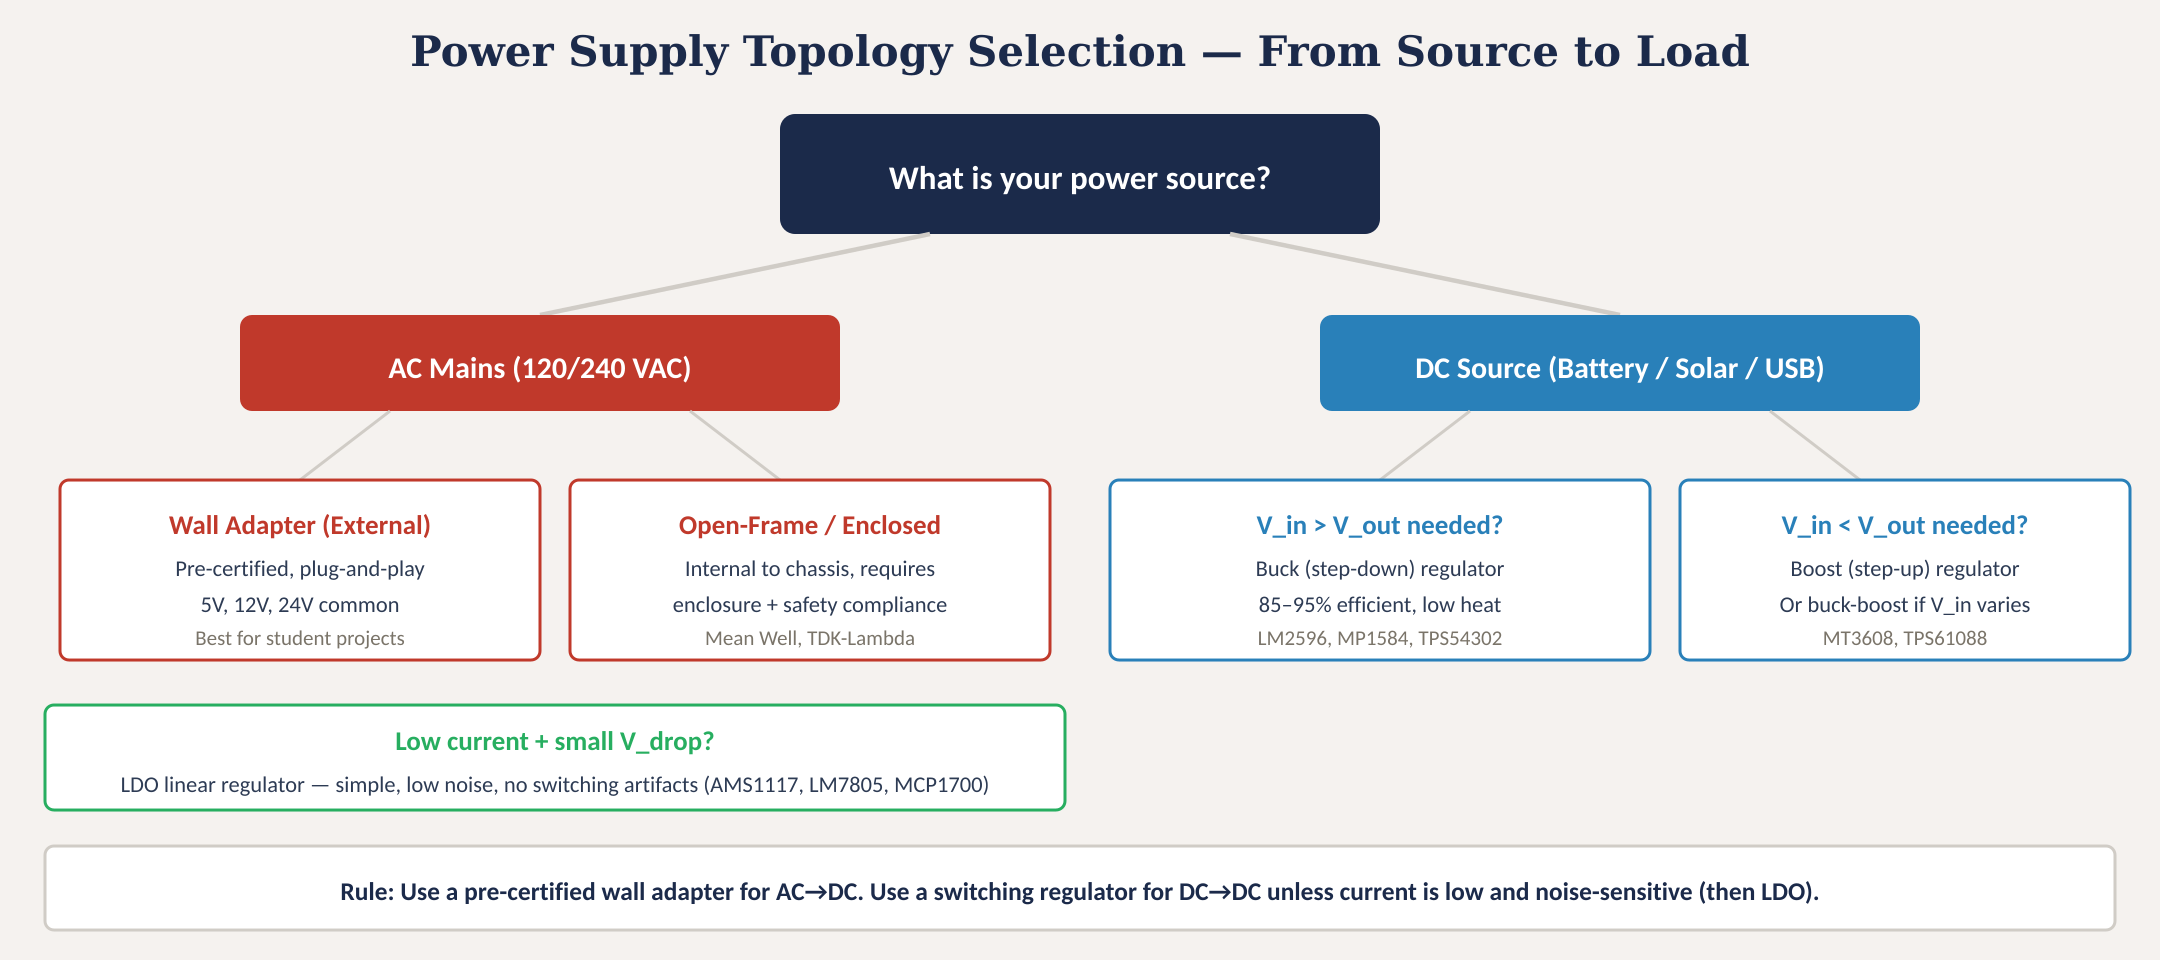
\includegraphics[width=\textwidth]{Power Supplies, Motors, and Pumps/fig_psu_topology.png}
\caption{Power supply topology decision tree --- from source type through voltage conversion to specific regulator selection.}
\label{fig:psu_topology}
\end{figure}


% ══════════════════════════════════════════════════════════════════════
\FloatBarrier
\section{DC Motors}
% ══════════════════════════════════════════════════════════════════════

\subsection{Motor Fundamentals}

Every DC motor operates on the Lorentz force: a current-carrying conductor in a magnetic field experiences a force. Two equations govern motor behavior:

\begin{align}
  \tau &= K_t \times I \quad \text{(torque is proportional to current)} \\
  V_{\text{back-EMF}} &= K_e \times \omega \quad \text{(back-EMF is proportional to speed)}
\end{align}

At stall ($\omega = 0$), back-EMF is zero and current is limited only by winding resistance: $I_{\text{stall}} = V / R_{\text{winding}}$. This is typically 6--10$\times$ the rated running current and causes rapid overheating.

\subsection{Brushed DC Motors}

Simplest motor type. Mechanical commutation via carbon brushes on a copper commutator. Apply voltage, it spins; reverse polarity, it reverses. Speed control via PWM. The torque-speed curve is linear from stall torque at zero speed to no-load speed at zero torque.

\textbf{Advantages}: Cheap, simple to drive (just PWM + H-bridge), widely available.

\textbf{Limitations}: Brush wear limits lifetime (1,000--5,000 hours), EMI from brush arcing, moderate efficiency (70--85\%).

\subsection{Brushless DC (BLDC) Motors}

Permanent magnets on the rotor, three-phase windings on the stator. An Electronic Speed Controller (ESC) sequentially energizes the stator phases. The motor \emph{cannot function without its ESC} --- they are an inseparable system.

\textbf{Advantages}: 85--95\% efficiency, 10,000+ hour life, higher power density, flat torque curve in the mid-range, lower EMI.

\textbf{Limitations}: Requires ESC (adds cost and complexity), cannot be driven directly from DC, commutation tuning matters.

\subsection{Stepper Motors}

Rotate in discrete angular steps (typically \ang{1.8} = 200 steps/rev). Open-loop positioning: count steps to know position without an encoder. NEMA 17 is the standard frame size for student projects. Driver boards (A4988, TMC2209) accept step/direction signals from any microcontroller.

\textbf{Advantages}: Precise positioning, high holding torque, no encoder needed.

\textbf{Limitations}: Torque drops rapidly with speed, runs hot (always energized), skips steps silently under overload.

\subsection{Servo Motors}

A motor + encoder + controller in a closed-loop system. Hobby servos (SG90, MG996R) are self-contained with PWM control. Industrial servos use BLDC motors with high-resolution encoders and dedicated controllers running PID loops at kHz rates.

\begin{figure}[ht!]
\centering
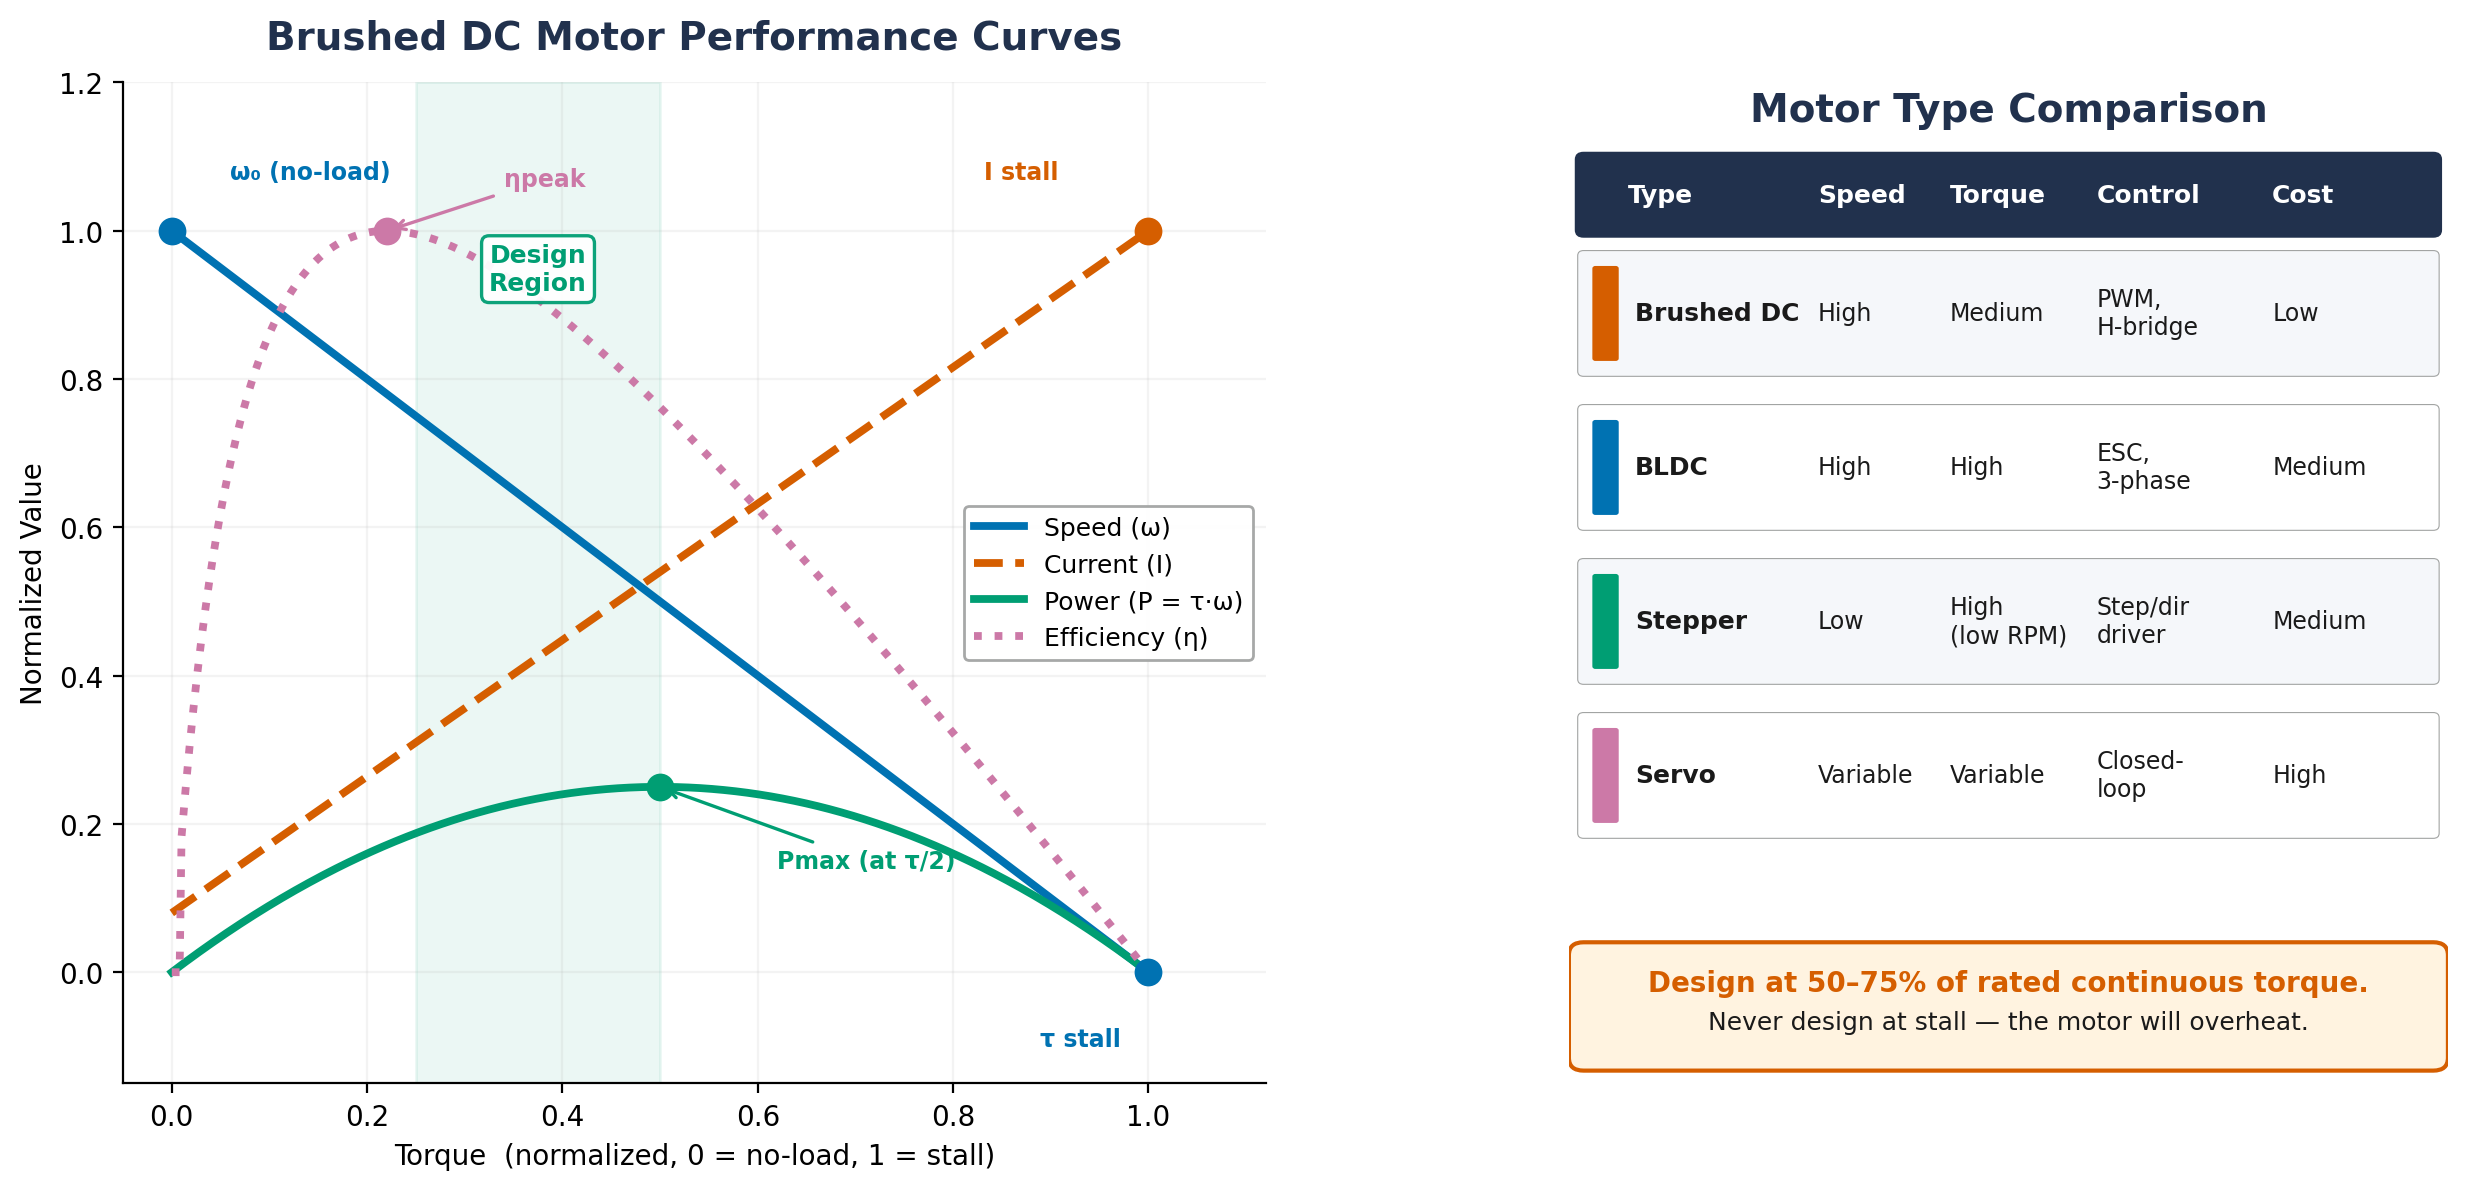
\includegraphics[width=\textwidth]{Power Supplies, Motors, and Pumps/fig_motor_curves.png}
\caption{Torque--speed characteristics for brushed DC (linear), BLDC (flat mid-range), and stepper (high-torque at low RPM) with comparison table.}
\label{fig:motor_curves}
\end{figure}

\subsection{Key Motor Specifications}

\begin{table}[ht!]
\centering\small
\begin{tabularx}{\textwidth}{l X}
  \toprule
  \textbf{Specification} & \textbf{Description} \\
  \midrule
  Rated Voltage & Nominal operating voltage. Must match your supply rail. \\
  No-Load Speed & Max speed with no load (RPM). Actual speed under load is lower. \\
  Stall Torque & Max torque at zero speed. \textbf{NOT your design point} --- stall current overheats the motor. \\
  Rated / Continuous Torque & Torque the motor delivers indefinitely. Your design ceiling. Derate to 50--75\%. \\
  Rated Current & Current at rated torque. Sizes your driver and power supply. \\
  Torque Constant ($K_t$) & Torque per ampere (\ensuremath{\text{N}\cdot\text{m}}/A). Calculate required current: $I = \tau_{\text{load}} / K_t$. \\
  \bottomrule
\end{tabularx}
\caption{Key motor specifications.}
\end{table}

\needspace{4\baselineskip}
\begin{warningbox}[Never Design at Stall Torque]
Stall current = $V_{\text{rated}} / R_{\text{winding}}$, typically 6--10$\times$ the rated running current. At stall, all electrical power converts to heat in the windings. A motor will overheat and fail within seconds to minutes. Always design at 50--75\% of the \emph{continuous} rated torque.
\end{warningbox}

\subsection{Motor Drive Electronics}
\label{sec:motor_drivers}

Every motor type needs a matched driver circuit:

\begin{itemize}[leftmargin=1.5em]
  \item \textbf{H-Bridge (Brushed DC)}: Four transistors for bidirectional current. L298N (2A, legacy), BTS7960 (43A), DRV8871 (3.6A). \textbf{Must include flyback diodes} --- back-EMF from inductive loads will destroy unprotected transistors.
  \item \textbf{ESC (BLDC)}: Converts DC + throttle signal to three-phase AC. Drone ESCs are cheap and widely available. Use bidirectional or 4-quadrant ESC for reversing.
  \item \textbf{Stepper Driver}: Converts step + direction signals into motor phase currents. A4988 (2A), DRV8825 (2.5A), TMC2209 (2A, silent). \textbf{Set the current limit potentiometer before powering on.}
  \item \textbf{Servo Controller}: Hobby servos need only a PWM signal (1--2\,ms pulse, 50\,Hz). Industrial servos require dedicated controllers.
\end{itemize}


% ══════════════════════════════════════════════════════════════════════
\FloatBarrier
\section{Pumps}
% ══════════════════════════════════════════════════════════════════════

\subsection{Positive Displacement vs.\ Dynamic}

\textbf{Positive displacement (PD)} pumps trap a fixed volume per cycle and force it into the discharge. Flow is proportional to speed and nearly independent of pressure. Self-priming. Pulsating flow. Types: gear, diaphragm, peristaltic, piston, vane.

\textbf{Dynamic (centrifugal)} pumps impart kinetic energy to the fluid via a spinning impeller. Flow varies with discharge pressure (follows a pump curve). Smooth, continuous flow. \emph{Not} self-priming. Best for high-volume, lower-pressure applications.

\subsection{Pump Types}

\subsubsection{Gear Pumps}
Two meshing gears trap fluid between teeth and housing. Self-priming, handles viscous fluids (oil, glycol). Constant flow rate. Used in hydraulic systems and lubrication. Primary failure mode: wear from particle contamination --- always use inline filtration.

\subsubsection{Diaphragm Pumps}
A flexible diaphragm oscillates to create suction and discharge. Seal-less design isolates fluid from moving parts. Self-priming, handles corrosive and abrasive fluids. Pulsating flow requires dampeners.

\subsubsection{Peristaltic Pumps}
Rollers compress a flexible tube, pushing fluid forward. Zero contamination risk --- fluid only contacts the tube. Easy maintenance: swap the tube. Gentle on shear-sensitive fluids. Limited to $\sim$30\,psi. Tube fatigue is the primary maintenance concern.

\subsubsection{Centrifugal / Impeller Pumps}
Spinning impeller accelerates fluid radially. Smooth, high-volume flow. Requires flooded suction (not self-priming). Poor with viscous fluids. Small 12V DC impeller pumps are widely available for student cooling and circulation projects.

\begin{figure}[ht!]
\centering
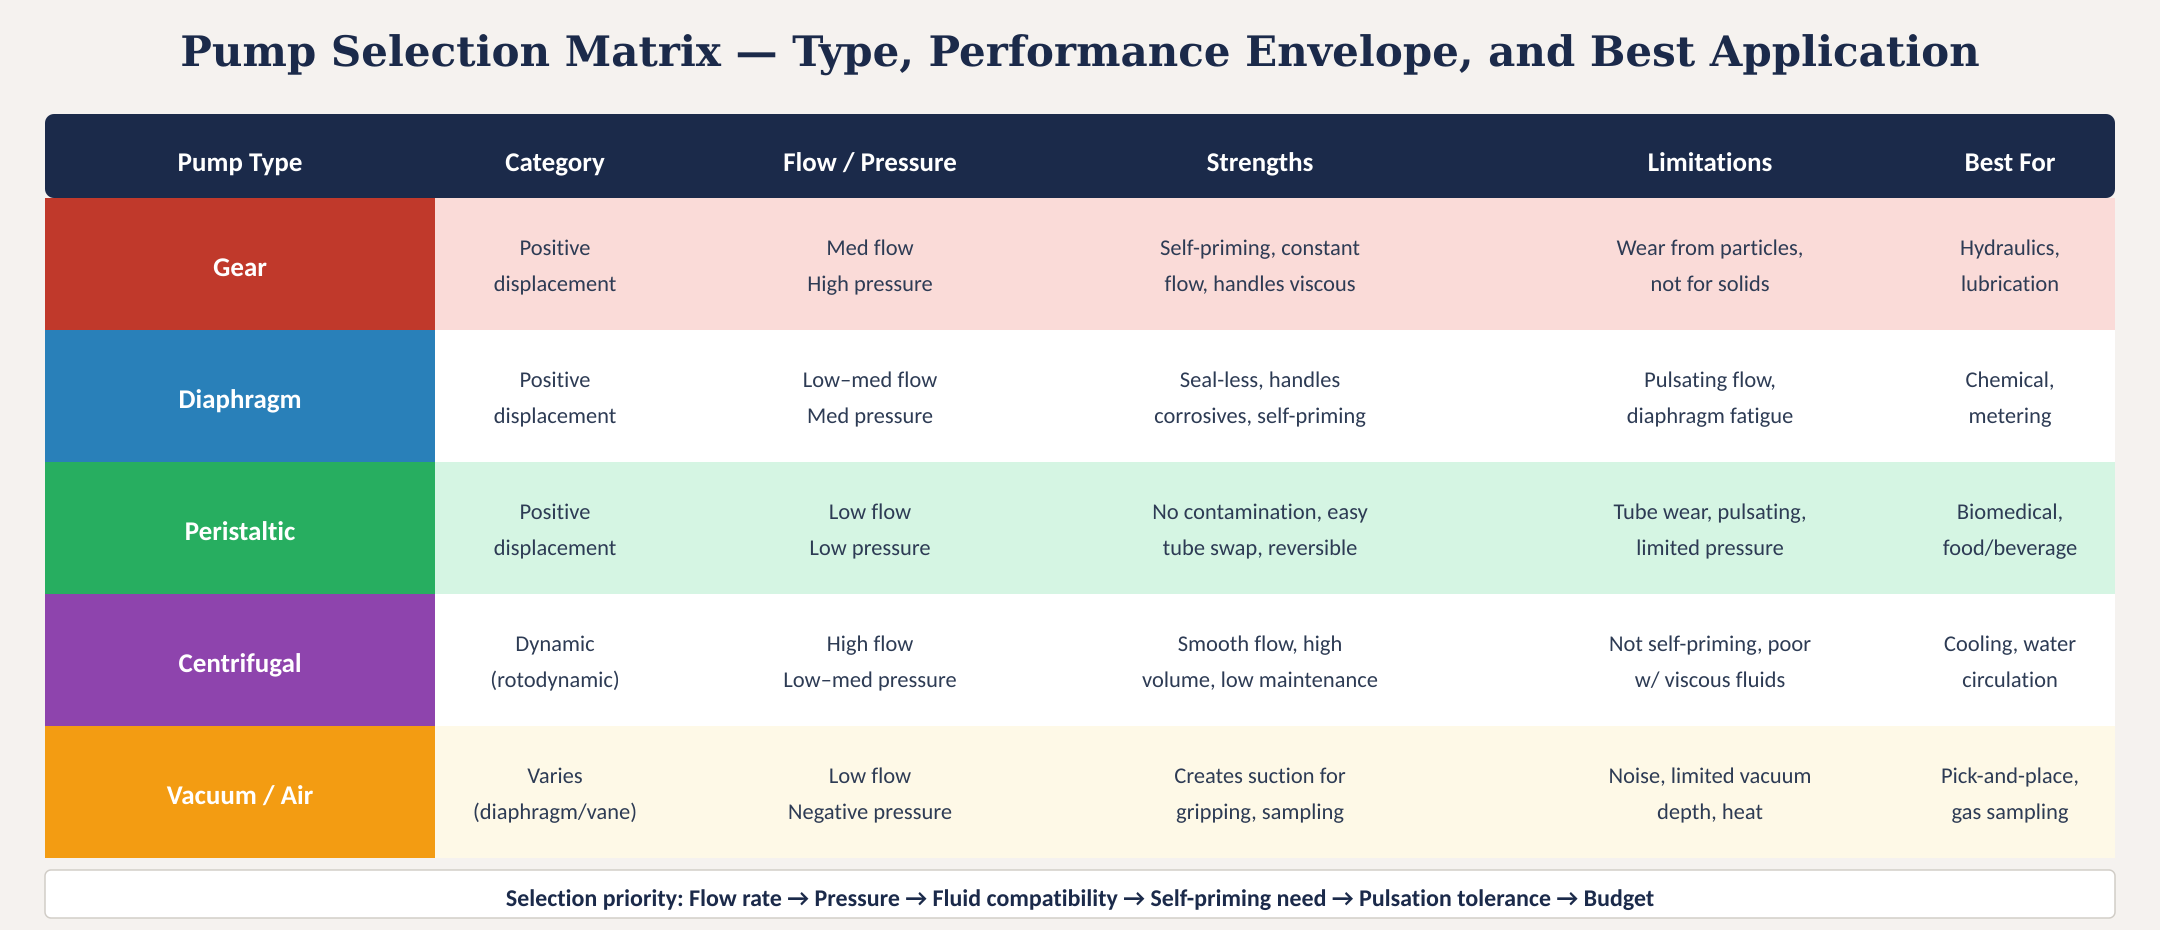
\includegraphics[width=\textwidth]{Power Supplies, Motors, and Pumps/fig_pump_matrix.png}
\caption{Pump selection matrix --- type, performance envelope, strengths, limitations, and best applications.}
\label{fig:pump_matrix}
\end{figure}

\subsection{Key Pump Specifications}

\begin{table}[ht!]
\centering\small
\begin{tabularx}{\textwidth}{l X}
  \toprule
  \textbf{Specification} & \textbf{Description} \\
  \midrule
  Flow Rate & Volume per unit time (L/min, mL/min). Must meet demand with $\geq$25\% margin. \\
  Discharge Pressure / Head & Max pressure (psi/bar) or total dynamic head (ft/m). Must exceed system losses. \\
  Fluid Compatibility & Wetted materials must be compatible with the pumped fluid. Check seal charts. \\
  Self-Priming & PD pumps: yes. Centrifugal: no (must be flooded). \\
  Motor Integration & Many small pumps include integrated 12V/24V DC motors --- specify the assembly. \\
  \bottomrule
\end{tabularx}
\caption{Key pump specifications.}
\end{table}


% ══════════════════════════════════════════════════════════════════════
\FloatBarrier
\section{Selection and Design Practice}
% ══════════════════════════════════════════════════════════════════════

\subsection{Unified Selection Framework}

\begin{figure}[ht!]
\centering
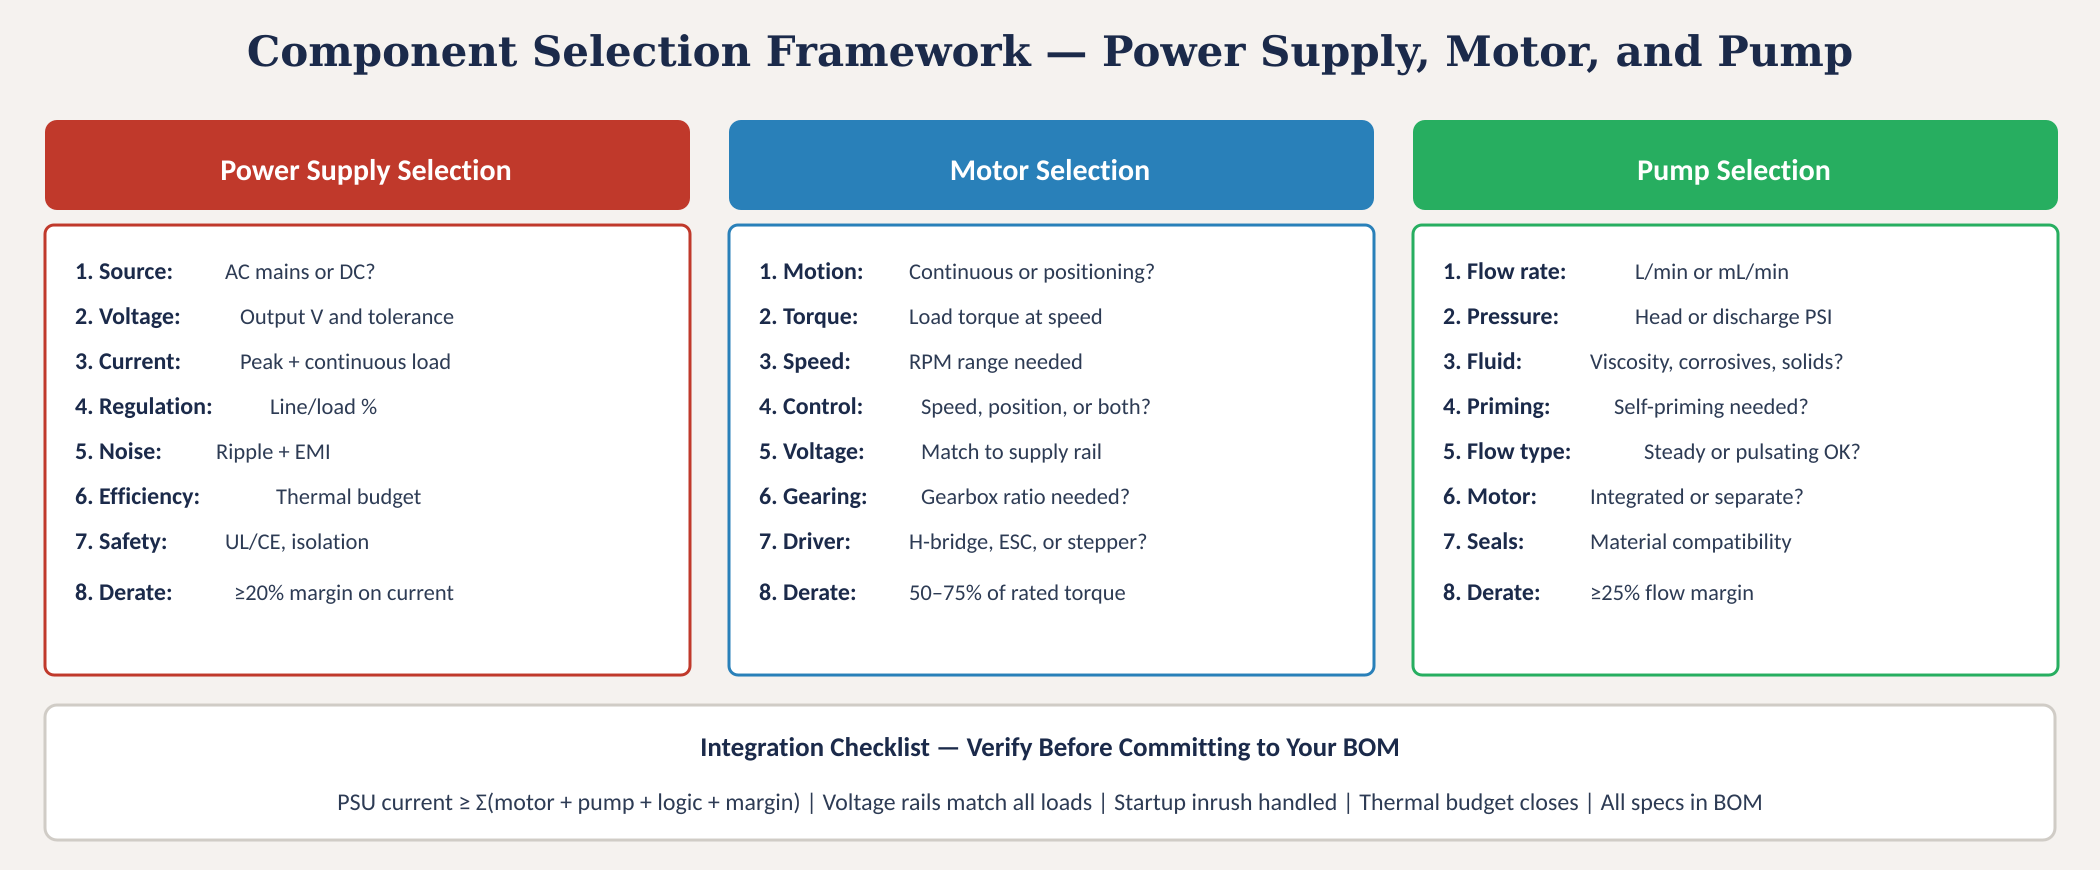
\includegraphics[width=\textwidth]{Power Supplies, Motors, and Pumps/fig_selection_framework.png}
\caption{Parallel selection flows for power supply, motor, and pump with integration verification checklist.}
\label{fig:selection_framework}
\end{figure}

\subsection{Design Rules}

\begin{enumerate}[leftmargin=1.5em]
  \item \textbf{Build a power budget spreadsheet first.} List every component with its voltage rail, continuous current, and peak current. Sum the columns. Add 25\% margin.
  \item \textbf{Calculate mechanical load torque before selecting a motor.} $\tau = F \times r$ for linear-to-rotary. Include friction, inertia, and acceleration torque. Select a motor with rated torque $\geq 1.5\times$ your load.
  \item \textbf{For fluid systems, map your complete flow circuit} --- pipe lengths, fittings, elevation, filters --- to calculate total system head loss. Select a pump whose curve crosses your system curve with margin.
  \item \textbf{Motor inrush is the \#1 power supply problem.} A motor rated at 2\,A running may draw 15\,A at startup. Size your supply for inrush, or use soft-start circuits.
  \item \textbf{Separate power and signal grounds.} Run motor power on dedicated wires back to the supply --- never share ground wires between motors and sensitive electronics.
  \item \textbf{Document everything in your BOM:} part number, manufacturer, voltage, current, torque, flow rate, and procurement source.
\end{enumerate}

\needspace{4\baselineskip}
\begin{keyconceptbox}[Five Key Takeaways]
\begin{enumerate}[nosep,leftmargin=1.5em]
  \item Power supplies: use pre-certified wall adapters for AC-DC; switching regulators for efficient DC-DC; LDOs only for low-current, noise-sensitive loads.
  \item Motors: match type to control need --- brushed DC for simplicity, BLDC for efficiency, stepper for open-loop positioning, servo for closed-loop precision. Every motor needs a driver.
  \item Pumps: positive displacement for precise flow and self-priming; centrifugal for high-volume smooth flow. Match wetted materials to your fluid.
  \item Derating is non-negotiable: 20\% current margin on power supplies, 25--50\% torque margin on motors, 25\% flow margin on pumps.
  \item Integration: build a power budget first, size for inrush, separate power and signal grounds, document every selection in your BOM.
\end{enumerate}
\end{keyconceptbox}


% ══════════════════════════════════════════════════════════════════════
\FloatBarrier
\section{Practice Questions}
% ══════════════════════════════════════════════════════════════════════

\subsection{Conceptual Questions}

\begin{enumerate}[leftmargin=1.5em]
  \item What is the fundamental difference between how a linear regulator and a switching regulator convert voltage?

  \item A 12\,V motor has a winding resistance of 0.$5\,\Omega$ and a rated current of 4\,A. What is the stall current? Why is this dangerous?

  \item Explain why a BLDC motor cannot function without an ESC, while a brushed DC motor can operate with just a battery connection.

  \item Your project needs to regulate a LiPo battery (3.0\,--4.2\,V) down to 3.3\,V. Why would a standard buck converter fail during battery discharge?

  \item Compare the self-priming capability of gear pumps versus centrifugal pumps. How does this affect installation design?

  \item Why must you include flyback diodes when driving a motor with an H-bridge? What happens without them?

  \item A power supply is rated at 10\,A at 25\,$^{\circ}$C. If your enclosure reaches 50\,$^{\circ}$C, can you still draw 10\,A? Explain.

  \item What is the primary advantage of a peristaltic pump over a gear pump for biomedical applications?
\end{enumerate}

\subsection{Application / Scenario Questions}

\begin{enumerate}[resume,leftmargin=1.5em]
  \item Your design uses a 24\,V wall adapter powering two DC motors (24\,V, 3\,A each running, 20\,A stall each) and an Arduino (5\,V, 200\,mA). Design the power architecture: what regulators are needed, what is the minimum supply current rating, and how do you handle motor inrush?

  \item You need to pump ethylene glycol coolant at 2\,L/min through a closed cooling loop with 3\,m of tubing, six fittings, and no elevation change. Which pump type do you recommend and why? What seal material?

  \item Your team selects a NEMA 17 stepper for a linear stage. The required force is 20\,N at 50\,mm/s using a 10\,mm lead screw. Calculate the required torque and verify whether a standard NEMA 17 (0.4\,\ensuremath{\text{N}\cdot\text{m}} rated) is adequate.

  \item \textbf{Diagnostic scenario}: Your prototype's motor operates normally when powered from a bench supply but stutters and resets the microcontroller when powered from the project's 12\,V battery pack. The battery is fully charged. What is the most likely cause, and how do you fix it?
\end{enumerate}

\subsection{Answers}

\begin{enumerate}[leftmargin=1.5em]
  \item A linear regulator dissipates excess voltage as heat (acts as a variable resistor). A switching regulator rapidly switches the input on/off and uses an inductor to transfer energy efficiently, achieving 85--95\% efficiency versus 40--80\% for linear.

  \item $I_{\text{stall}} = V/R = 12/0.5 = 24\,A$ --- six times the rated current. At stall, all 288\,\text{W} ($24 \times 12$) converts to heat in the windings. The motor will overheat and fail within seconds.

  \item A brushed DC motor has mechanical commutation (brushes and commutator) that automatically reverses current in the rotor windings. A BLDC motor's rotor has permanent magnets and the stator windings must be energized in a precise three-phase sequence by the ESC, which reads rotor position via Hall sensors or back-EMF sensing. Without the ESC, there is no commutation and no rotation.

  \item A buck converter requires $V_{\text{in}} > V_{\text{out}}$ to regulate. When the LiPo discharges below 3.3\,V (which happens as the cell depletes toward 3.0\,V), the buck cannot maintain the output. A buck-boost converter is required because it handles the input crossing the output voltage.

  \item Gear pumps are self-priming: they can draw fluid up from below the pump inlet by creating suction through the gear tooth spaces. Centrifugal pumps are not self-priming and require a flooded suction (pump inlet below fluid level). This means centrifugal pumps must be installed below the tank or use a foot valve and check valve to maintain prime.

  \item A motor is an inductive load. When current is suddenly switched off, the collapsing magnetic field generates a voltage spike (back-EMF) that can be many times the supply voltage. Without flyback diodes, this spike destroys the H-bridge transistors. Flyback diodes clamp the spike by providing a current path for the decaying magnetic energy.

  \item No. Every power supply has a thermal derating curve. At 50\,$^{\circ}$C, the supply has less thermal headroom to dissipate heat. A typical derating might reduce capacity to 70--80\% of the 25\,$^{\circ}$C rating, meaning 7\,--8\,A. Always check the datasheet derating curve.

  \item The fluid in a peristaltic pump only contacts the inside of a disposable tube --- no seals, rotors, or metal surfaces touch the fluid. This eliminates contamination risk and allows easy sterilization by swapping the tube. A gear pump has fluid contact with gears, housing, and shaft seals, making sterilization far more difficult.

  \item Architecture: wall adapter provides 24\,V rail directly to motors via H-bridges. A buck converter (e.g., LM2596) steps 24\,V down to 5\,V for the Arduino. Minimum supply current: continuous = $2 \times 3 + 0.2 = 6.2\,A$, but inrush = $2 \times 20 = 40\,A$ simultaneously. A 10\,A supply with bulk capacitance ($\geq$4700\,$\mu$F) on the motor rail to absorb inrush, plus staggered motor startup in firmware (start one motor, wait 500\,ms, start the second), is the practical solution.

  \item A small DC centrifugal impeller pump is appropriate: the loop is closed (no priming issue if pump is at the bottom), flow is moderate, ethylene glycol is low viscosity, and smooth non-pulsating flow is preferred for cooling. Seal material: Viton (FKM) or EPDM --- both compatible with ethylene glycol at moderate temperatures.

  \item Torque = force $\times$ lead / ($2\pi \times$ efficiency). $\tau = 20 \times 0.010 / (2\pi \times 0.9) = 0.035\,\ensuremath{\text{N}\cdot\text{m}}$. The NEMA 17 at 0.4\,\ensuremath{\text{N}\cdot\text{m}} rated torque provides $0.4 / 0.035 = 11.4\times$ margin. However, at the required speed: $50\text{ mm/s} / 10\text{ mm/rev} = 5\text{ rev/s} = 300\text{ RPM}$. Check the stepper's torque-speed curve at 300 RPM --- torque typically drops to 40--60\% of holding torque, giving 0.16\,--0.24\,\ensuremath{\text{N}\cdot\text{m}}. Still adequate ($4.6$--$6.9\times$ margin), but verify on the actual datasheet curve.

  \item Most likely cause: the battery cannot supply the motor inrush current. Unlike a bench supply (which can deliver virtually unlimited current), a battery has internal resistance. During motor startup, the inrush current ($6$--$10\times$ running) causes a voltage drop across the battery's internal resistance, drooping the 12\,V rail. If it drops below the buck converter's minimum input or the microcontroller's brown-out threshold ($\sim$2.7\,V for most AVR/ARM), the MCU resets. Fix: add a large bulk capacitor ($\geq$4700\,$\mu$F) on the battery rail close to the motor driver, use a battery with lower internal resistance (higher C-rating), implement soft-start in firmware, and add a separate regulated supply for the MCU with adequate input capacitance.
\end{enumerate}


% ══════════════════════════════════════════════════════════════════════

\FloatBarrier
\chapter{Power Architecture \& Circuit Safety}

\vspace{1em}




\vspace{1em}


% ══════════════════════════════════════════════════════════════════════
\FloatBarrier
\section{Power Architecture}
\label{sec:arch}
% ══════════════════════════════════════════════════════════════════════

\subsection{System-Level Design}

A well-designed power system flows from source through three functional stages before reaching the loads. The \textbf{input stage} is where power enters through a single, well-defined connector. This is where you place first-line protections: a keyed connector (prevents miswiring), reverse polarity protection, an input fuse, and a TVS diode for transient suppression. The \textbf{regulation stage} converts raw input voltage into the specific rails your system needs --- commonly cascading from the highest voltage down (e.g., 24\,V input $\to$ 12\,V motor rail $\to$ 5\,V sensor rail $\to$ 3.3\,V MCU rail). The \textbf{distribution stage} delivers regulated power to each load through individual protection --- per-rail fuses or electronic current limiters that prevent a fault in one subsystem from cascading.

\begin{figure}[ht!]
\centering
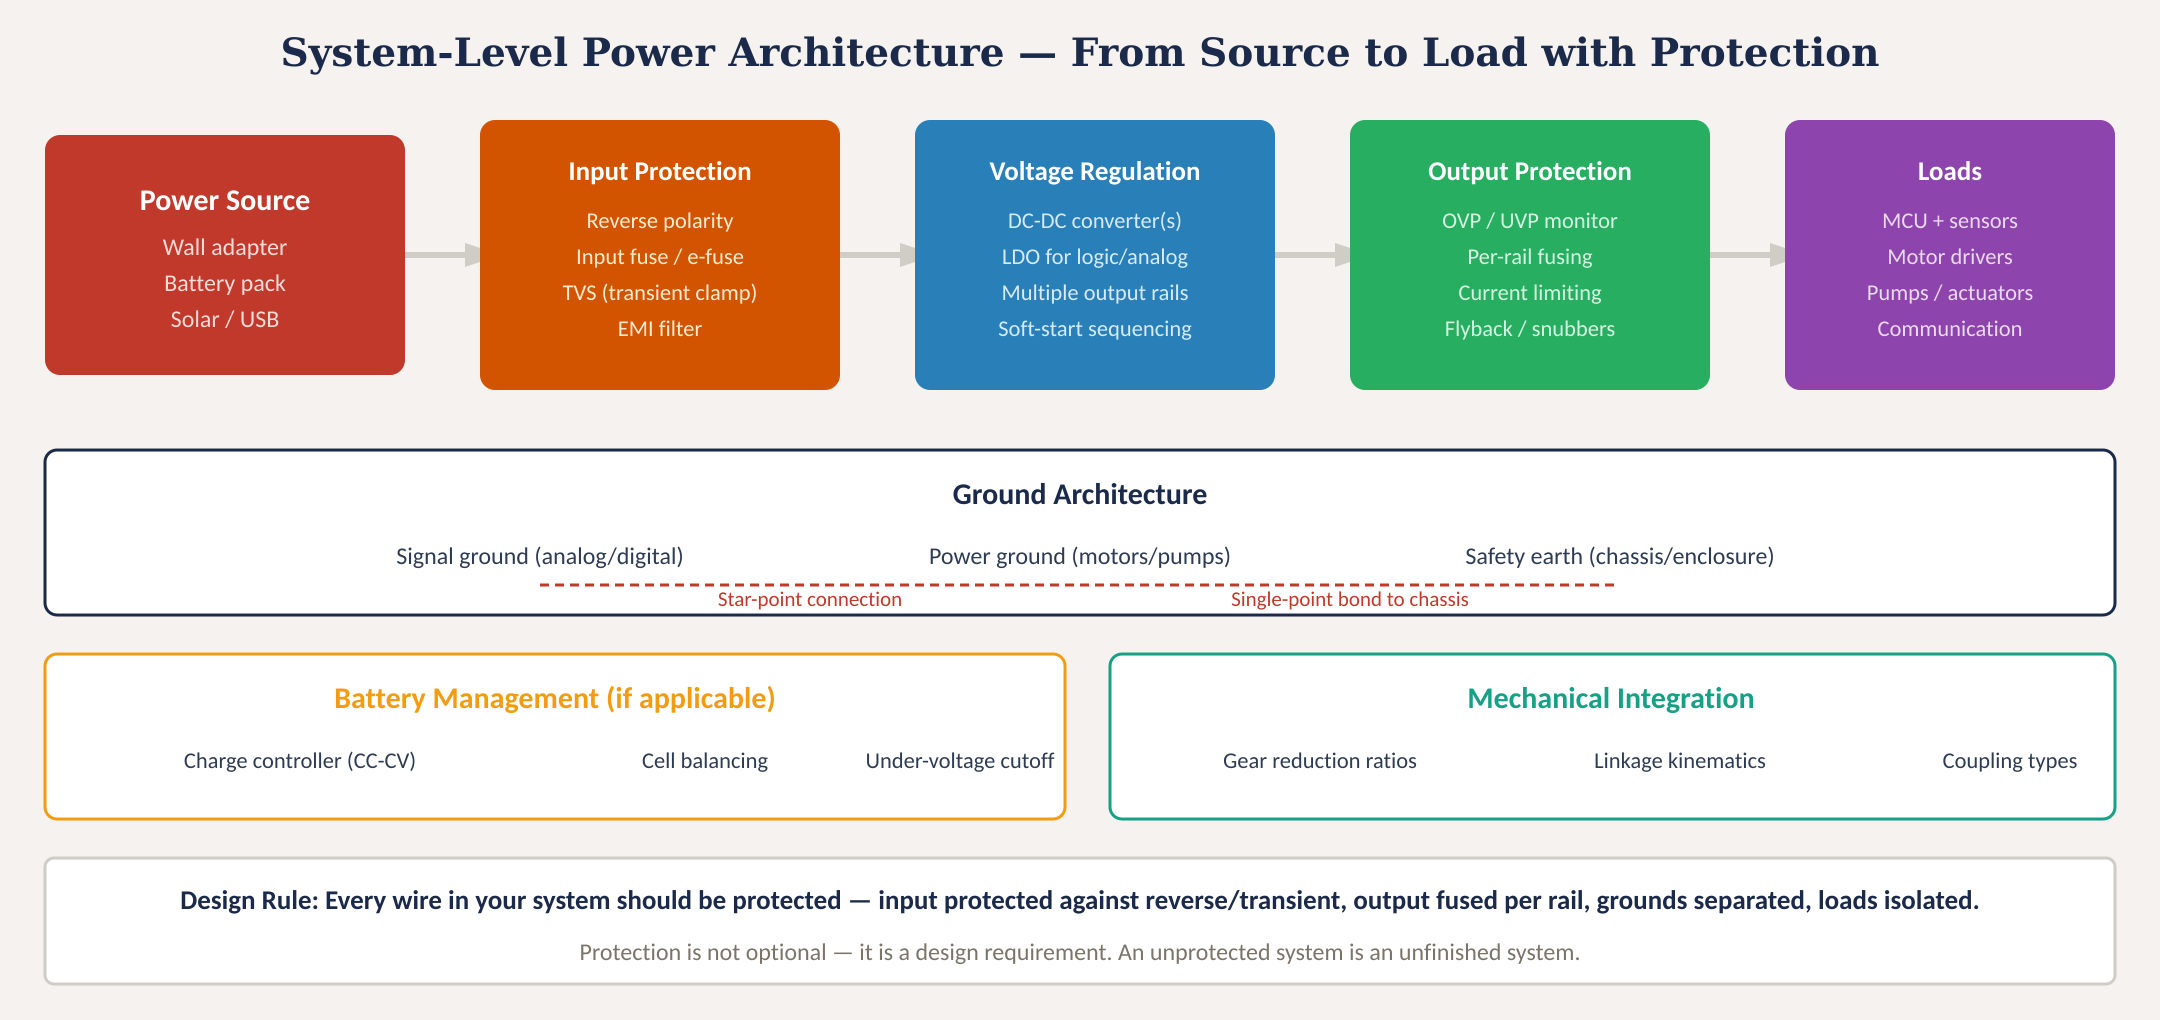
\includegraphics[width=\textwidth]{Power Architecture/fig_power_architecture.png}
\caption{System-level power architecture from source to load with protection stages, ground architecture, battery management, and mechanical integration.}
\label{fig:architecture}
\end{figure}

\subsection{Grounding Strategy}
\label{sec:grounding}

Ground is not a magical zero-volt reference --- it is a real conductor with real resistance and inductance. When a motor draws 5\,A through a ground trace with $50\mohm$ resistance, there is a 250\,mV drop along that trace. If your ADC's ground reference shares that path, your sensor readings are corrupted.

\subsubsection{Star-Point Grounding}
Run separate ground conductors from each subsystem back to a single point near the power supply. Motor ground, sensor ground, and MCU ground each get their own conductor. They meet at \emph{one star point}. This prevents motor return current from flowing through sensor ground paths.

\subsubsection{Three Ground Domains}
\begin{itemize}[nosep,leftmargin=1.5em]
  \item \textbf{Signal ground}: analog sensors, ADCs, digital logic. Low current, noise-sensitive.
  \item \textbf{Power ground}: motors, pumps, solenoids, heaters. High current, noisy.
  \item \textbf{Safety earth}: metal enclosure, chassis. Fault-current path for AC-powered systems.
\end{itemize}

\needspace{4\baselineskip}
\begin{warningbox}[The \#1 Debugging Time Sink]
Poor grounding is the single most common cause of difficult-to-diagnose intermittent failures in student projects. If your sensor readings are noisy, your MCU resets when a motor starts, or your serial communication drops characters --- check your grounding first.
\end{warningbox}

\subsubsection{AC Mains Safety}
Use a Class~II (double-insulated) wall adapter whenever possible --- no earth ground connection is needed. If you must use an internal open-frame supply, bond the metal enclosure to earth ground through a 3-prong inlet with proper strain relief. \textbf{Never defeat a ground prong.}

\subsubsection{Signal Isolation}
Use optocouplers or digital isolators (Si8620, ADUM1201) to pass signals between high-voltage and low-voltage domains. Essential when controlling AC loads (relays, triacs) from a microcontroller.


\subsection{Battery Integration}
\label{sec:battery}

Lithium cells (LiPo, Li-ion, LiFePO\textsubscript{4}) store enormous energy density and can cause fire or explosion if mishandled. A Battery Management System (BMS) is \textbf{mandatory}:

\begin{itemize}[nosep,leftmargin=1.5em]
  \item Overcharge cutoff: 4.2\,V/cell maximum.
  \item Deep-discharge cutoff: 3.0\,V/cell minimum (irreversible damage below this).
  \item Overcurrent / short-circuit shutoff.
  \item Cell balancing for multi-cell packs.
\end{itemize}

Common modules: TP4056 (single-cell charger, CC-CV profile), BQ25895 (buck-boost charger IC), BQ76940 (multi-cell BMS). During development, always store and charge lithium batteries in a fireproof LiPo-safe bag. \textbf{Never charge unattended without a BMS.}

\needspace{4\baselineskip}
\begin{tipbox}[DC Generation Sources (Solar, Alternator)]
Solar panels produce variable voltage --- use an MPPT charge controller to extract maximum power. Always include a blocking diode to prevent battery discharge through the panel at night. For alternators: rectify the AC output, regulate with a charge controller, and add TVS/MOV protection against load-dump voltage spikes if the battery disconnects while the alternator is running.
\end{tipbox}


% ══════════════════════════════════════════════════════════════════════
\FloatBarrier
\section{Protection Circuits}
\label{sec:protection}
% ══════════════════════════════════════════════════════════════════════

The philosophy is \textbf{defense in depth}: layer multiple protections so that each catches what the previous one missed. No single device guards against all threats.

\begin{figure}[ht!]
\centering
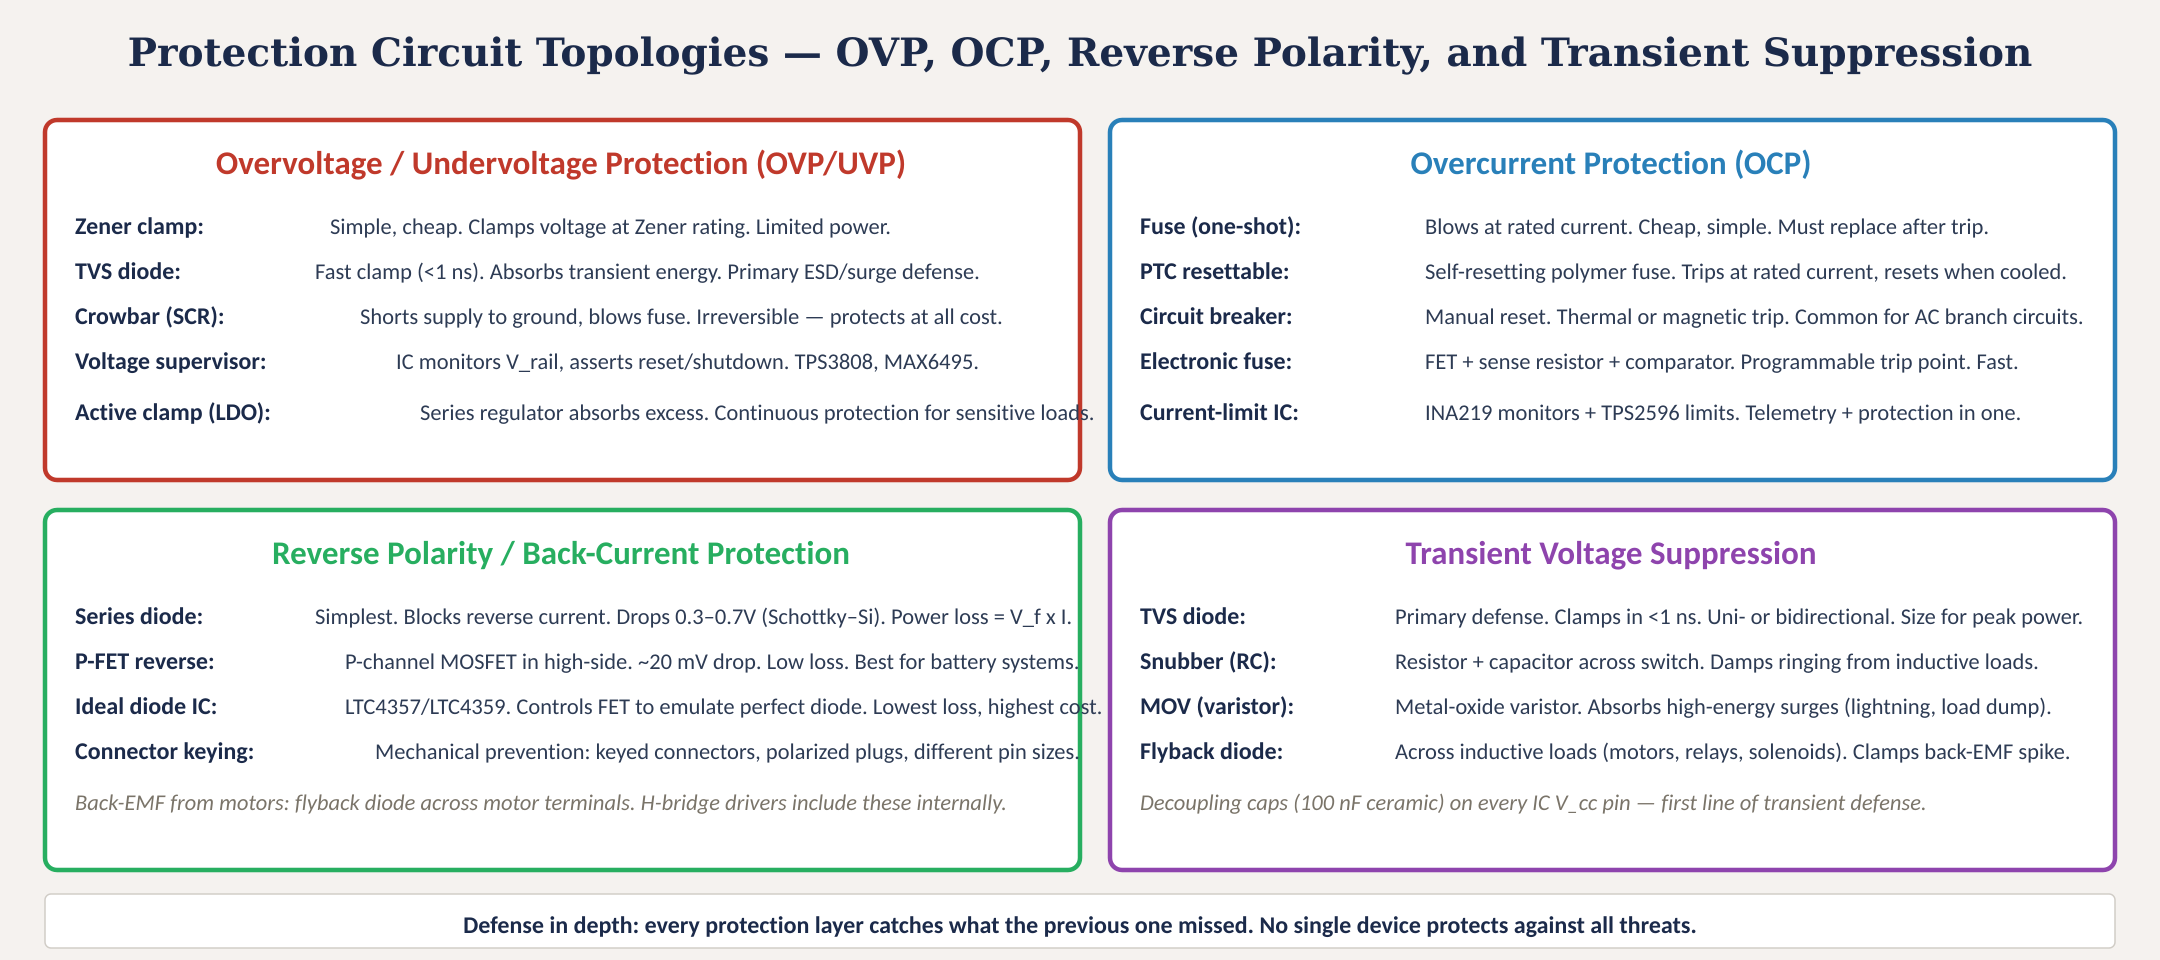
\includegraphics[width=\textwidth]{Power Architecture/fig_protection_topologies.png}
\caption{Four protection categories: OVP/UVP, OCP, reverse polarity/back-current, and transient suppression with specific device options.}
\label{fig:protection}
\end{figure}


\subsection{Overvoltage and Undervoltage Protection (OVP / UVP)}

\textbf{Overvoltage} pushes components beyond absolute maximum ratings --- gate oxide breakdown, latch-up, permanent damage. \textbf{Undervoltage} causes unpredictable behavior: brown-outs, corrupted flash memory, and erratic execution.

\subsubsection{Zener Clamp}
A Zener diode across the supply rail conducts when voltage exceeds its breakdown value, clamping the rail. Simple and cheap but limited by power dissipation ($P = (V_{\text{spike}} - V_Z) \times I$). Select $V_Z$ slightly above your nominal rail (e.g., 5.6\,V Zener for a 5\,V rail).

\subsubsection{TVS Diode}
A Transient Voltage Suppressor --- essentially a heavy-duty bidirectional Zener optimized for high peak power. Responds in $<$1\,\,ns. The primary defense against ESD, inductive spikes, and power supply transients. \textbf{Every power input in a professional design has a TVS diode.}

\textbf{Selection}: standoff voltage $\geq$ operating voltage; clamping voltage $<$ component absolute maximum rating. Common series: SMAJ, SMBJ, 1.5KE.

\subsubsection{Voltage Supervisor IC}
Monitors the supply rail and asserts a reset or shutdown signal when voltage is out of range. Does not clamp --- it shuts the system down gracefully. Essential for microcontroller brown-out protection. Common: TPS3808 (adjustable OVP/UVP), MAX6495 (OVP with FET control), TLV803 (simple reset).

\subsubsection{Crowbar Circuit}
An SCR (thyristor) fires when voltage exceeds a threshold, shorting the supply to ground and blowing the upstream fuse. \textbf{Irreversible} --- the fuse must be replaced. Used as a last resort when the overvoltage source has enough sustained energy to overwhelm a clamp.


\subsection{Overcurrent Protection (OCP)}
\label{sec:ocp}

Every power rail must have current limiting. A short circuit without protection delivers the full energy of the supply into the fault.

\subsubsection{Fuses (One-Shot)}
A fusible element melts at its rated current. \textbf{Fast-blow} for sensitive electronics; \textbf{slow-blow} (time-delay) for motor circuits where inrush exceeds steady-state. The fuse must blow \emph{before} the wire or component is damaged. Must be accessible for replacement.

\subsubsection{PTC Resettable Fuses}
Polymer PTC (positive temperature coefficient) devices. Resistance increases dramatically at the trip point, limiting current. Self-resets when cooled. Slower than traditional fuses. Best for USB ports and sensor circuits where the fault is intermittent.

\subsubsection{Electronic Fuses (eFuse)}
A MOSFET in series with the load, controlled by a current-sense amplifier. Programmable trip point, fast response, automatic retry or latched shutdown. Provides current \emph{limiting} (not just cutting) --- can hold current at a safe level during motor inrush. Common: TPS2596, LTC4368, MAX14690.

\subsubsection{Circuit Breakers}
Thermal or magnetic trip mechanism with manual reset. Common for AC branch circuits (15\,A, 20\,A per NEC). In DC systems, used for battery main disconnects. \textbf{Must be DC-rated} --- an AC breaker may not safely interrupt DC arcs because DC does not cross zero.

\needspace{4\baselineskip}
\begin{warningbox}[Fuse + Wire Sizing Rule]
The fuse must blow before the wire overheats. This means the fuse rating must be \emph{below} the wire's ampacity. Size them together using NEC Table 310.16 or AWG ampacity charts: the fuse protects the wire, the wire carries the current, and the load defines the requirement.
\end{warningbox}


\subsection{Reverse Polarity and Back-Current Protection}
\label{sec:reverse}

A battery connected backwards forward-biases body diodes of every downstream MOSFET and IC, often destroying the entire board in milliseconds.

\subsubsection{Series Diode}
Simplest approach. A Schottky diode ($\sim$0.3\,V drop) or silicon diode ($\sim$0.7\,V drop) in the positive rail blocks reverse current. Power loss = $V_f \times I_{\text{load}}$. Best for low-current ($<$2\,A) circuits where the voltage drop is acceptable.

\subsubsection{P-Channel MOSFET}
A P-FET in the high-side power path conducts when polarity is correct (body diode initially conducts, pulling gate low, fully enhancing the FET) and blocks when reversed. Voltage drop = $I \times R_{DS(\text{on})}$, typically 10\,--$50\mohm$. At 5\,A with $20\mohm$: only 0.1\,V drop, 0.5\,\text{W} loss. \textbf{Best for battery-powered systems.} Common: Si2301, IRLML6402, DMG2307L.

\subsubsection{Ideal Diode IC}
An IC controlling an external N-FET to emulate a perfect diode with $\sim$20\,mV forward drop. Lowest loss, fastest reverse blocking, highest cost. LTC4357, LTC4359, MAX40200. Also used for OR-ing redundant supplies and solar/battery combining.

\subsubsection{Mechanical Prevention}
Keyed connectors, polarized plugs, and different-sized pins physically prevent reverse connection. The first line of defense --- always use polarized connectors for DC power.


\subsection{Transient Voltage Suppression}
\label{sec:transient}

Every time you switch an inductive load --- motor, relay, solenoid --- you create a voltage transient. The physics: $V = -L \times dI/dt$. Current cannot change instantaneously in an inductor, so the collapsing magnetic field generates a spike that can reach hundreds of volts from a 12\,V motor.

\begin{figure}[ht!]
\centering
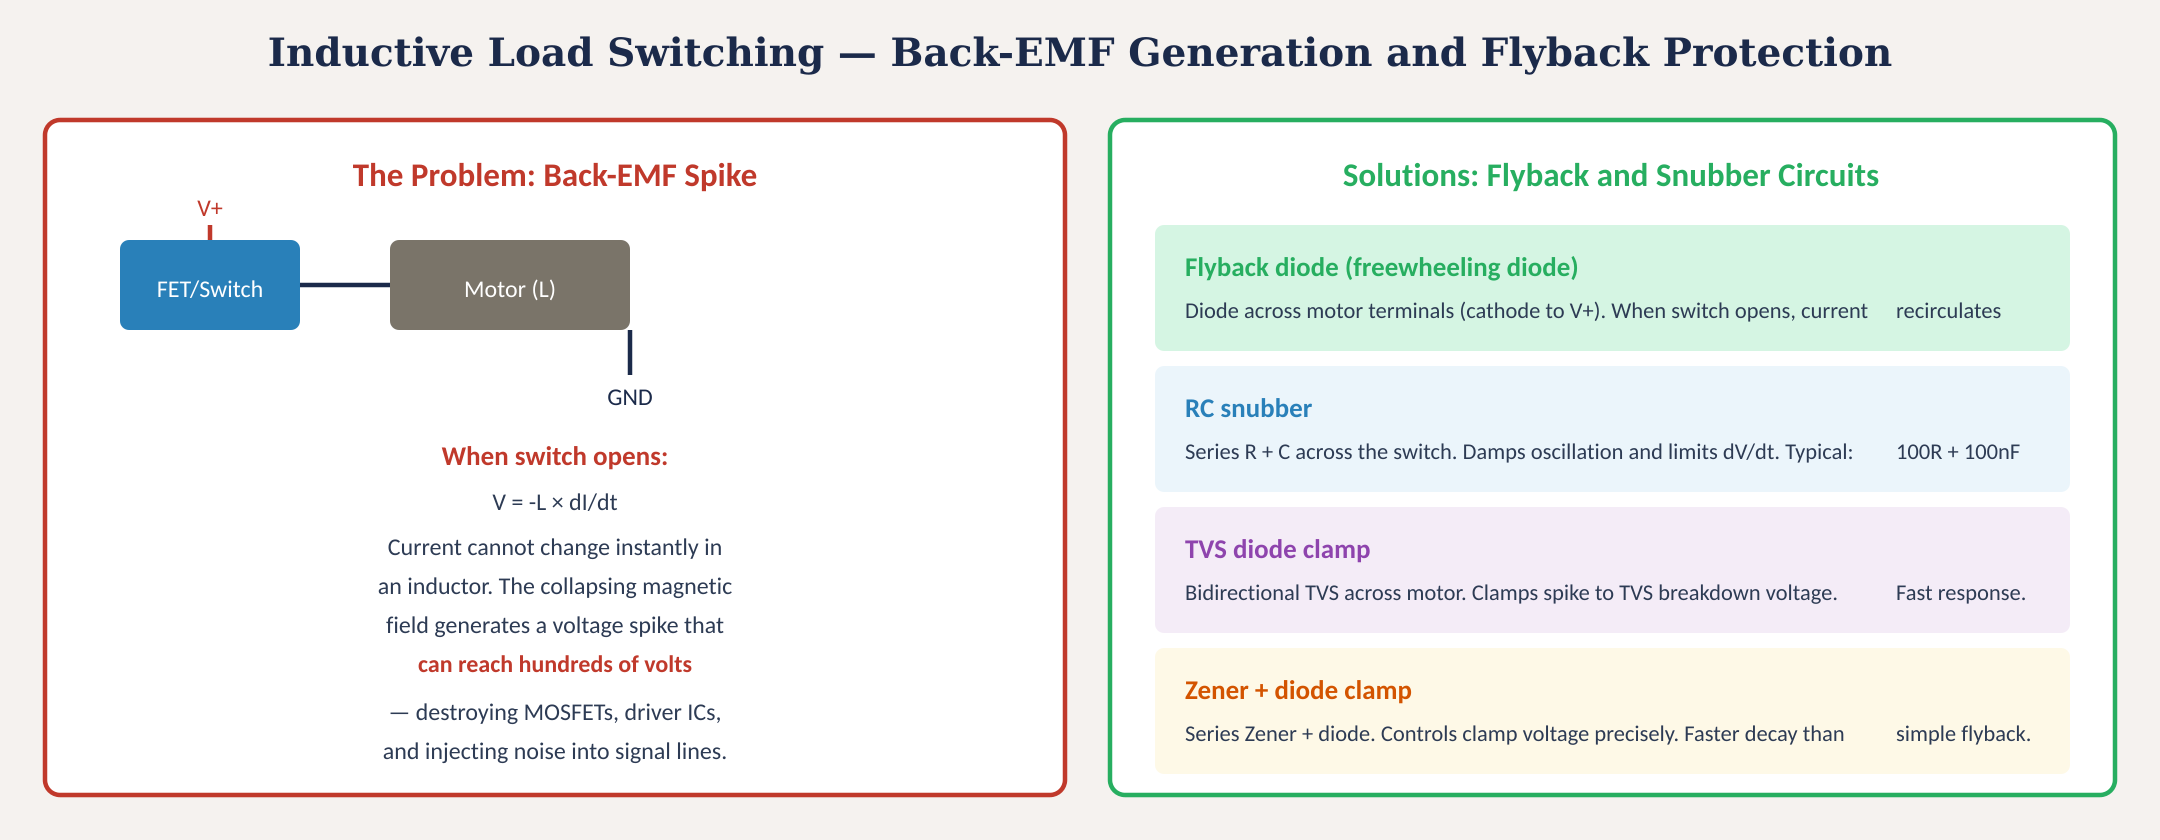
\includegraphics[width=\textwidth]{Power Architecture/fig_back_emf.png}
\caption{Back-EMF generation from inductive load switching and four protection solutions: flyback diode, RC snubber, TVS clamp, and Zener+diode.}
\label{fig:backemf}
\end{figure}

\subsubsection{Flyback Diode (Freewheeling Diode)}
\textbf{The single most important protection for inductive loads.} A diode across the motor, relay, or solenoid (cathode to V+) provides a current path when the switch opens. Without it, the collapsing field generates a spike that destroys the switching device. Use a fast-recovery or Schottky diode. H-bridge driver ICs include these internally, but if you drive a relay or solenoid with a bare MOSFET, you \textbf{must} add one externally.

\subsubsection{RC Snubber}
A resistor-capacitor network across a switch or relay contact. The capacitor absorbs the initial spike; the resistor dissipates energy and damps oscillation. Typical starting values: $100\,\Omega$ + $100$\,nF for relay contacts. Tune by observing the transient on an oscilloscope.

\subsubsection{TVS Diode (Board-Level)}
Place a TVS across each power rail at the board edge where external cables connect. Absorbs energy from ESD, cable transients, and motor switching spikes propagating through the power bus.

\subsubsection{Decoupling Capacitors}
100\,\,nF ceramic capacitors on \textbf{every} IC $V_{CC}$ pin, as close to the pin as physically possible. These absorb high-frequency transients before they reach the IC. For power regulators, add bulk capacitance (10\,--100\,$\mu$F) per the datasheet. \textbf{Decoupling is not optional.}


% ══════════════════════════════════════════════════════════════════════
\FloatBarrier
\section{Electromechanical Integration}
\label{sec:mechint}
% ══════════════════════════════════════════════════════════════════════

Electrical power must ultimately be converted to mechanical work. The interface between the electrical system (Chapter~8) and the mechanical load is where power architecture meets physical reality. For detailed coverage of gear trains, belt drives, chains, shafts, couplings, lead screws, and linkages, see the \textbf{Mechanical Power Transmission} chapter. For fasteners, bearings, and mounting, see the \textbf{Mechanical Fasteners \& Bearings} chapter. This section covers the integration principle that links them.

\begin{figure}[ht!]
\centering
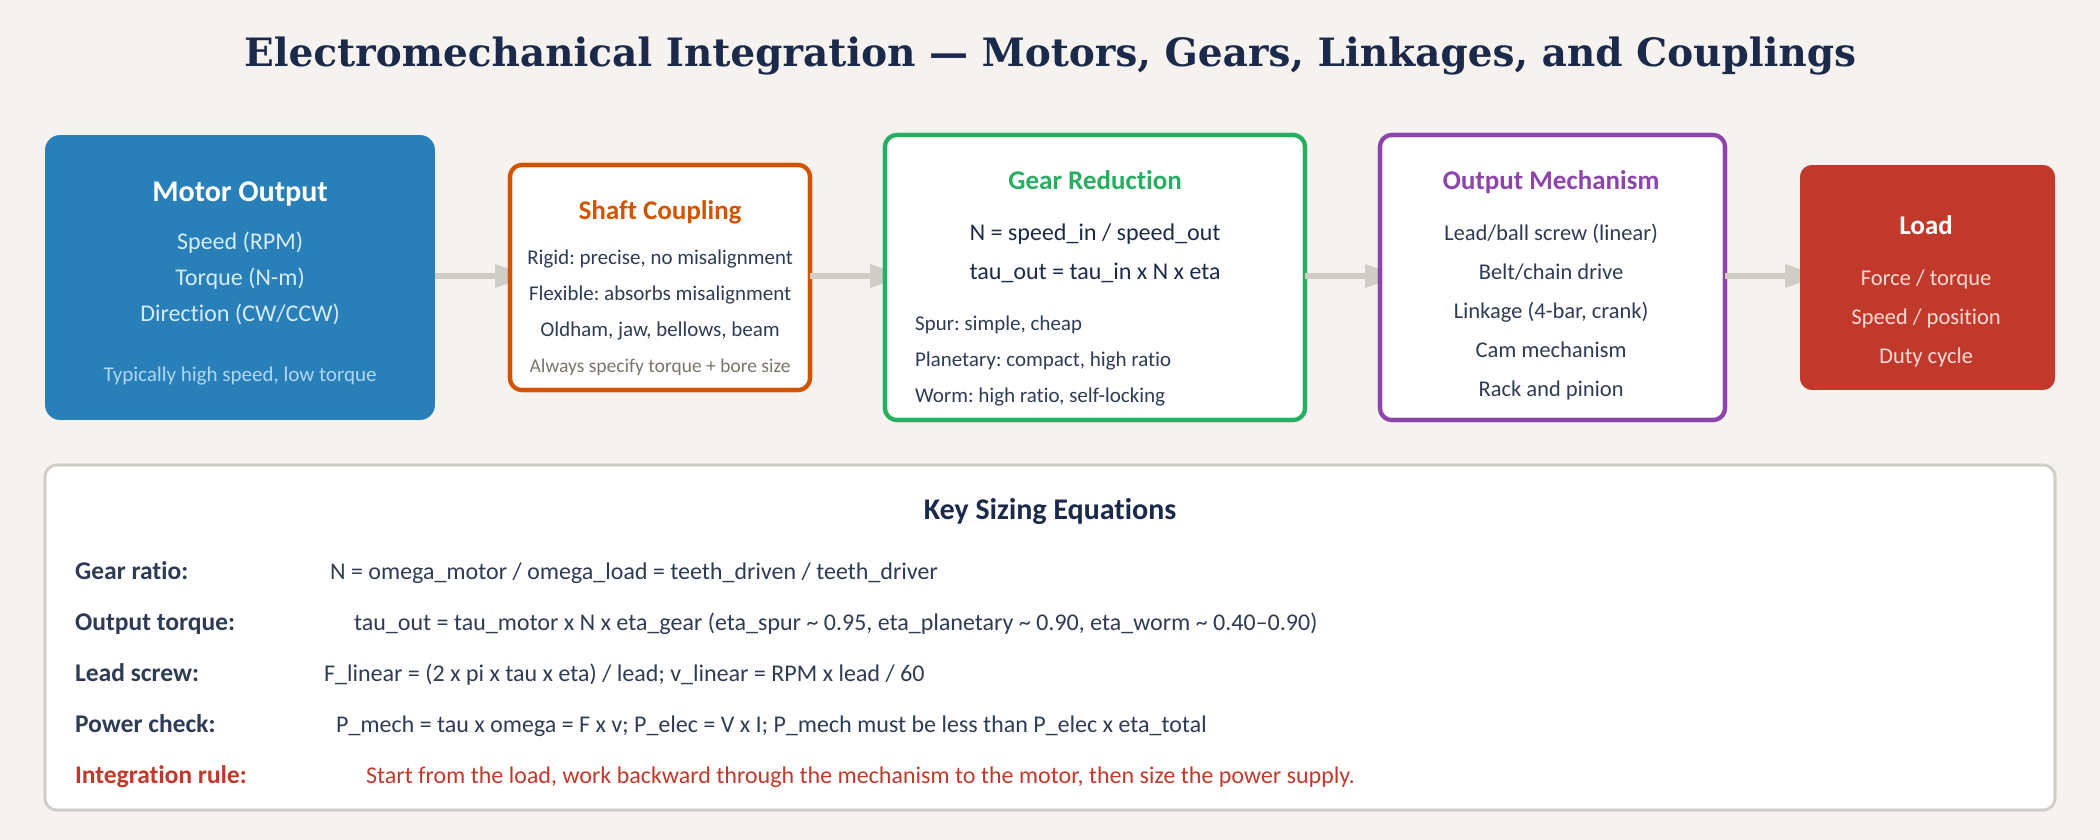
\includegraphics[width=\textwidth]{Power Architecture/fig_mech_integration.png}
\caption{Motor-to-load power flow through coupling, gear reduction, and output mechanism with key sizing equations.}
\label{fig:mech}
\end{figure}

\needspace{4\baselineskip}
\begin{keyconceptbox}[The Integration Rule: Start from the Load]
\textbf{Always design backward from the load}: calculate the force/torque and speed the load requires $\to$ select the transmission mechanism and gear ratio (Mechanical Power Transmission chapter) $\to$ calculate the required motor torque $\to$ select the motor (Chapter~8) $\to$ calculate the current draw $\to$ size the power supply and protection circuits (this chapter). The power check at every stage: $P_{\text{mech}} = \tau \omega = F v$ must be $\leq P_{\text{elec}} \times \eta_{\text{total}}$. If the numbers do not close, resize from the load backward---never from the motor forward.
\end{keyconceptbox}


% ══════════════════════════════════════════════════════════════════════
\FloatBarrier
\section{Safety Design Checklist}
\label{sec:checklist}
% ══════════════════════════════════════════════════════════════════════

Every item must be addressed before commissioning:

\begin{enumerate}[leftmargin=1.5em]
  \item Input has reverse polarity protection (P-FET or series diode).
  \item Input has a fuse or electronic current limiter rated for expected peak current.
  \item TVS diode on every power input where external cables connect.
  \item Voltage supervisor on MCU power rail (brown-out reset).
  \item Flyback diode on every inductive load not protected by the driver IC.
  \item Per-rail fusing --- each output rail has its own current protection.
  \item 100\,\,nF decoupling capacitor on every IC $V_{CC}$ pin.
  \item Signal and power grounds separated, joined at a single star point.
  \item Enclosure bonded to earth ground (if using internal AC-DC supply).
  \item All wire gauges sized for their maximum current with appropriate derating.
\end{enumerate}


% ══════════════════════════════════════════════════════════════════════
\FloatBarrier
\section{Practice Questions}
\label{sec:practice}
% ══════════════════════════════════════════════════════════════════════

\subsection{Conceptual Questions}

\begin{enumerate}[leftmargin=1.5em]
  \item Explain why star-point grounding prevents motor noise from corrupting ADC readings. What happens if motor current returns through a shared ground trace?

  \item A TVS diode has a standoff voltage of 12\,V and a clamping voltage of 19.9\,V at 10\,A. Is this suitable for protecting a 12\,V circuit whose components have a 20\,V absolute maximum rating?

  \item Compare a series Schottky diode versus a P-channel MOSFET for reverse polarity protection at 5\,A. Calculate the power loss for each (Schottky $V_f = 0.3\,V$, P-FET $R_{DS(\text{on})} = 20\,\mohm$).

  \item Why must a DC circuit breaker be specifically rated for DC voltage? What is the hazard of using an AC-rated breaker on a DC circuit?

  \item A relay coil has 50\,\text{mH} inductance and draws 100\,mA at 12\,V. If the switch opens in 1\,$\mu$s, estimate the back-EMF spike voltage ($V = L \times dI/dt$). Why does this destroy a 60\,V MOSFET?

  \item What is the difference between a crowbar circuit and a TVS diode clamp? When would you use each?

  \item Explain why decoupling capacitors must be placed as close to the IC power pin as possible, not just ``somewhere on the same board.''
\end{enumerate}

\subsection{Application / Scenario Questions}

\begin{enumerate}[resume,leftmargin=1.5em]
  \item Your robot uses a 4S LiPo battery (14.8\,V nominal, 16.8\,V max charge, 12.0\,V cutoff) powering two DC motors (5\,A each continuous, 30\,A each stall), a Raspberry Pi (5\,V, 2.5\,A), and three servos (6\,V, 1\,A each peak). Design the complete power architecture: draw a block diagram showing every rail, regulator, and protection device. Specify part numbers where possible.

  \item Your capstone team's prototype works perfectly on the bench but fails intermittently in the field. Symptoms: the motor runs fine, but the microcontroller occasionally resets, and analog sensor readings drift by 200\,mV when the motor switches direction. Diagnose the root cause and propose a fix using concepts from this module.

  \item A classmate argues that a flyback diode is unnecessary because ``the motor driver IC already handles back-EMF.'' Under what conditions is the classmate correct? Under what conditions is the classmate dangerously wrong?

  \item Design a protection scheme for a solar panel (18\,V open-circuit, 5\,A short-circuit) charging a 3S LiPo (11.1\,V nominal) that also powers a 12\,V water pump. Include reverse-current blocking, charge control, and load protection.
\end{enumerate}

\subsection{Answers}

\begin{enumerate}[leftmargin=1.5em]
  \item In a shared ground, motor current ($I_M$) flows through the same trace as sensor return current. The trace has resistance $R$, so the sensor sees a ground voltage offset of $V_{\text{noise}} = I_M \times R$. With star-point grounding, motor current returns through its own dedicated conductor, so the sensor ground conductor carries only the small sensor current. The noise voltage on the sensor ground drops from $I_M \times R$ to $I_{\text{sensor}} \times R$, which is typically orders of magnitude smaller.

  \item Yes --- the standoff voltage (12\,V) is at or above the operating voltage, so the TVS does not conduct during normal operation. The clamping voltage (19.9\,V) is below the 20\,V absolute maximum, so the TVS clamps before the components are damaged. However, the margin is very tight (0.1\,V). A TVS with a 16.7\,V or lower clamping voltage would provide better margin. Always verify the clamping voltage at the expected peak current, not just the rated value.

  \item Schottky: $P = V_f \times I = 0.3 \times 5 = 1.5\,\text{W}$. P-FET: $P = I^2 \times R_{DS} = 25 \times 0.020 = 0.5\,\text{W}$. The P-FET dissipates one-third the power. At 5\,A, the Schottky also drops the voltage rail by 0.3\,V, which may push the rail below the minimum operating voltage of downstream components. The P-FET drops only 0.1\,V. For battery-powered systems where efficiency and voltage headroom matter, the P-FET is strongly preferred.

  \item AC current crosses zero 120 times per second (at 60\,Hz), which naturally extinguishes any arc at the breaker contacts. DC current never crosses zero, so a DC arc can sustain indefinitely. An AC-rated breaker's contacts and arc chute may not be designed to extinguish a sustained DC arc, potentially causing the breaker to fail to interrupt the circuit --- or worse, catch fire internally.

  \item $V = L \times dI/dt = 0.050 \times (0.100 / 0.000001) = 5000\,V$. This 5\,kV spike (in theory) far exceeds the 60\,V MOSFET's drain-source breakdown voltage. In practice, the MOSFET avalanches and the spike is clamped at the breakdown voltage, but the energy dissipated during avalanche can destroy the device. A flyback diode clamps the spike to approximately $V_{\text{supply}} + V_f \approx 12.7\,V$, well within the MOSFET's rating.

  \item A TVS diode \emph{clamps} the voltage --- it conducts just enough to limit the voltage and absorbs the transient energy, then stops conducting when the voltage returns to normal. Operation is non-destructive. A crowbar circuit \emph{shorts} the supply to ground via an SCR, deliberately blowing the upstream fuse. It is destructive (fuse replacement required) but provides guaranteed protection when the overvoltage has enough sustained energy to overwhelm a TVS. Use TVS for transient spikes (ESD, inductive switching); use crowbar for sustained overvoltage from a failed regulator.

  \item Decoupling caps work by providing a low-impedance path for high-frequency transients to bypass the IC rather than entering through the power pins. The trace between the capacitor and the IC pin has inductance proportional to its length. A long trace adds enough inductance to negate the capacitor's effectiveness at high frequencies. Placing the cap within a few millimeters of the pin minimizes this parasitic inductance and keeps the bypass impedance low at the frequencies where transients occur.

  \item Architecture: Battery $\to$ main fuse (80\,A --- covers dual motor stall) $\to$ reverse polarity P-FET (IRLML6402 or similar) $\to$ TVS diode (18\,V standoff) $\to$ power distribution bus. Motor rail: direct from battery through individual 40\,A slow-blow fuses per motor, H-bridge drivers with integrated flyback diodes. 5\,V rail: buck converter (e.g., LM2596 or MP1584, 3A rated) from battery bus, with 100\,$\mu$F bulk cap + 100\,\,nF ceramic decoupling. 6\,V servo rail: buck converter (adjustable output set to 6\,V, 5A rated --- TPS54560) with per-servo PTC fuses. BMS: 4S BMS module with 12.0\,V cutoff, 16.8\,V overcharge protection, and cell balancing. Grounds: star-point near main fuse; separate motor ground bus and logic ground bus.

  \item Root cause: ground-coupled motor noise. When the motor reverses direction via the H-bridge, the current transient creates a voltage spike on the shared ground that (a) momentarily shifts the MCU's ground reference, triggering a brown-out reset, and (b) offsets the ADC's reference voltage by 200\,mV, corrupting readings. Fix: (a)~separate motor power ground and MCU signal ground, joining at a star point near the battery; (b)~add a voltage supervisor (TPS3808) on the MCU rail to hold the MCU in clean reset during transients rather than allowing corrupted execution; (c)~add bulk capacitance (470\,$\mu$F) on the MCU's supply rail to absorb the transient; (d)~add a TVS diode on the motor power bus.

  \item The classmate is correct when using a properly rated H-bridge driver IC (like L298N, DRV8871, BTS7960) that includes integrated flyback/freewheeling diodes across the output MOSFETs. These diodes handle the back-EMF from the motor. The classmate is \textbf{dangerously wrong} when: (a)~driving a relay, solenoid, or valve directly from a bare MOSFET or BJT --- these loads have no integrated protection; (b)~the motor's back-EMF exceeds the driver's clamping capability; or (c)~using a driver module where the ``protection diodes'' are actually for the logic section, not the motor outputs. \textbf{Rule}: verify in the driver's datasheet that flyback diodes are explicitly rated for the motor's inductive energy.

  \item Solar input: blocking diode (Schottky, e.g., MBR2045) prevents battery discharge through panel at night. MPPT charge controller (e.g., Genasun GV-5 or Victron 75/15) sized for 3S LiPo with 12.6\,V charge termination. Reverse polarity: P-FET on both the solar input and the battery connector. TVS diode (18\,V standoff) on the solar input for transient protection. Load: battery feeds pump through a slow-blow fuse (3\,A for a 2\,A pump). Flyback diode across pump motor terminals. Voltage supervisor monitors battery voltage and disables pump via a load switch when battery drops below 10.5\,V to protect cells. The charge controller's MPPT algorithm ensures maximum solar harvest even as panel voltage varies with sun angle and temperature.
\end{enumerate}


% ══════════════════════════════════════════════════════════════════════


\FloatBarrier
\chapter{Mechanical Fasteners \& Bearings}

\vspace{1em}

\begin{keyconceptbox}[Bottom Line]
Every mechanical system is held together by fasteners and supported by bearings. Selecting the wrong bolt grade, under-torquing a critical joint, or choosing a bearing that cannot handle the load will cause your system to fail --- often catastrophically and without warning. This chapter covers the fastener and bearing knowledge you need to specify these components correctly in your BOM and engineering drawings.
\end{keyconceptbox}

\vspace{1em}

\FloatBarrier
\section{Threaded Fasteners}

\subsection{Bolt and Screw Anatomy}
A threaded fastener converts rotational torque into axial clamping force (preload) that holds a joint together. The key geometric parameters are: \textbf{nominal diameter} (the major diameter of the thread, e.g., M6 = 6\,mm, 1/4-20 = 0.250\,in), \textbf{pitch} (distance between adjacent threads --- metric specifies pitch directly in mm; imperial uses threads per inch, TPI), \textbf{thread length} (the portion of the shank that is threaded), and \textbf{head type} (hex, socket, flat, pan, button --- each serves a different function and requires a different tool).

\textbf{Bolts vs.\ screws}: A bolt passes through a clearance hole and is secured by a nut on the other side. A screw threads directly into a tapped hole in one of the parts being joined. The distinction matters because a bolt can be tightened from one side while a screw requires access to the hole side for assembly.

\subsection{Thread Standards}

\begin{table}[ht!]
\centering\small
\begin{tabularx}{\textwidth}{l l X l}
\toprule
\textbf{Standard} & \textbf{Designation} & \textbf{Description} & \textbf{Example} \\
\midrule
Metric Coarse & M $\times$ pitch & Default metric; pitch implied if omitted & M6 (= M6$\times$1.0) \\
Metric Fine & M $\times$ pitch & Smaller pitch for precision, thin walls, vibration & M6$\times$0.75 \\
UNC (Unified Coarse) & dia-TPI & Default imperial; general purpose & 1/4-20 \\
UNF (Unified Fine) & dia-TPI & Finer pitch; stronger in thin materials & 1/4-28 \\
\bottomrule
\end{tabularx}
\caption{Common thread standards.}
\end{table}

\needspace{4\baselineskip}
\begin{warningbox}[Metric and Imperial Do Not Mix]
An M6$\times$1.0 bolt will \emph{appear} to start threading into a 1/4-20 nut but will cross-thread and strip after 2--3 turns. The diameters are close (6.0\,mm vs.\ 6.35\,mm) but the thread forms are incompatible. Cross-threading destroys both parts. Always verify thread standard before assembly --- if it does not turn freely by hand for at least 3 full turns, stop.
\end{warningbox}

\subsection{Bolt Grades and Strength Classes}

\begin{figure}[ht!]\centering
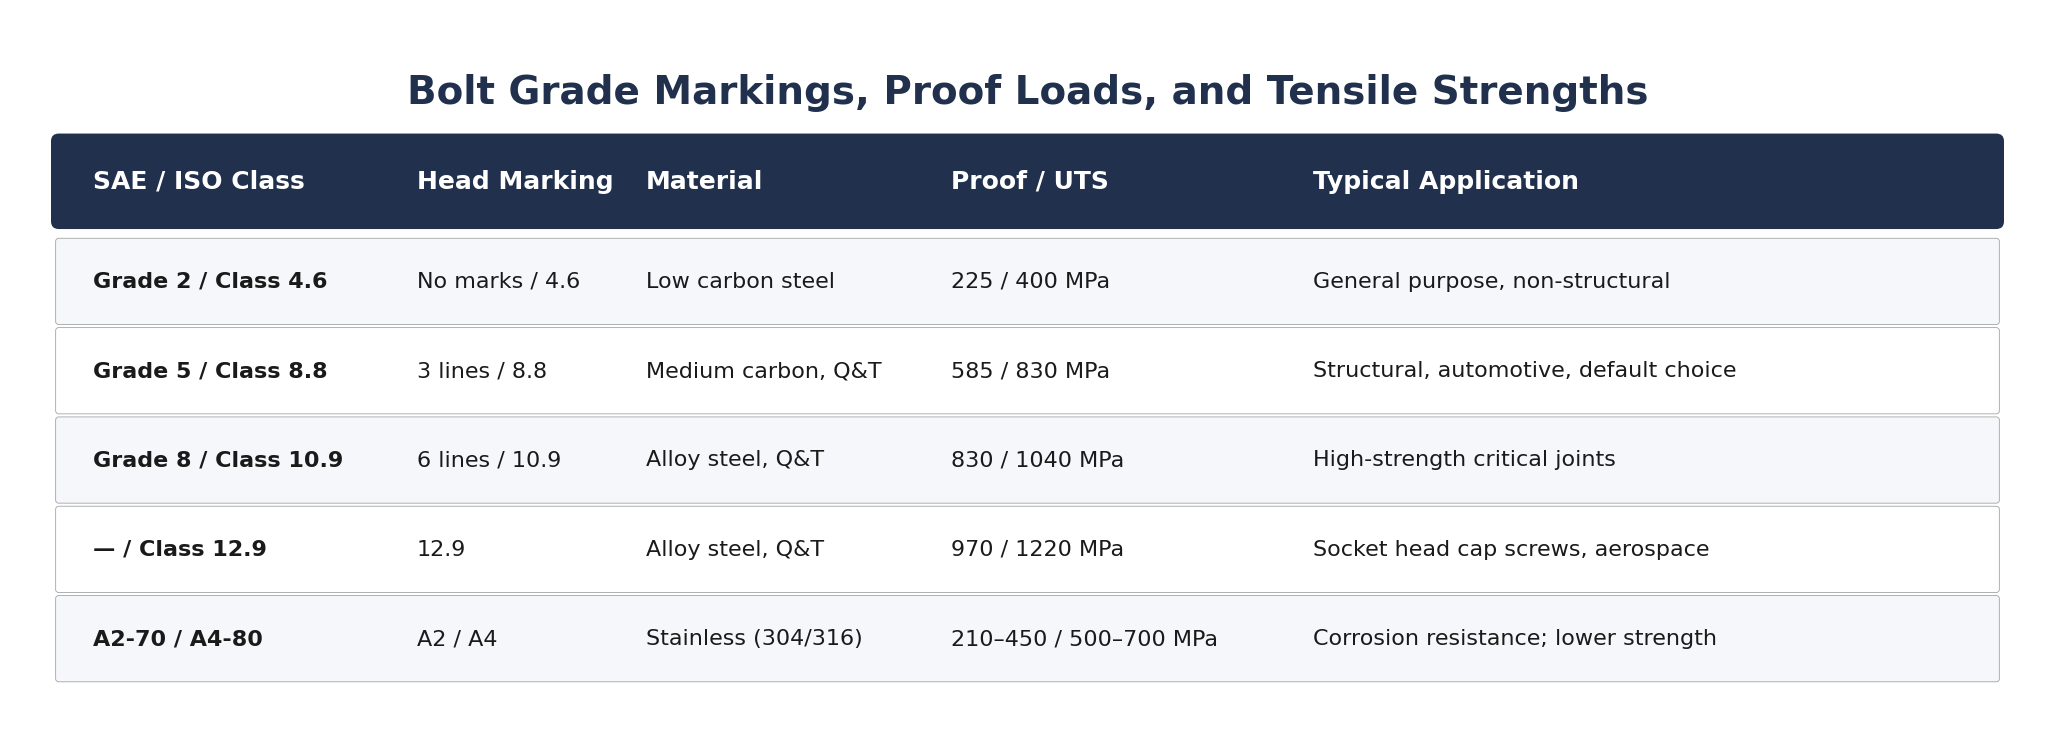
\includegraphics[width=\textwidth]{Mechanical Fasteners and Bearings/fig_fastener_grades.png}
\caption{Bolt grade markings, proof loads, and tensile strengths for SAE and ISO metric classes.}\label{fig:grades}
\end{figure}

\textbf{SAE grades} (imperial): Grade~2 (low carbon, no markings, general purpose), Grade~5 (medium carbon, 3 radial lines, structural), Grade~8 (alloy steel, 6 radial lines, high-strength critical joints). \textbf{ISO metric classes}: Class~4.6 ($\approx$ Grade~2), Class~8.8 ($\approx$ Grade~5), Class~10.9 ($\approx$ Grade~8), Class~12.9 (highest strength, socket head cap screws).

The class designation directly encodes strength: for Class~8.8, the first digit $\times$ 100 = ultimate tensile strength in MPa ($800$\,MPa), and first $\times$ second $\times$ 10 = yield strength in MPa ($8 \times 8 \times 10 = 640$\,MPa). Proof load (the maximum load without permanent deformation) is approximately 90\% of yield.

\needspace{4\baselineskip}
\begin{tipbox}[Specify the Grade]
In your BOM and engineering drawings, always specify the fastener grade: ``M6$\times$1.0$\times$20, Class~8.8, zinc plated.'' A drawing that says only ``M6 bolt'' allows the machine shop to use the cheapest hardware-store fastener, which may be Class~4.6 --- half the strength you designed for. Grade~8.8 (metric) or Grade~5 (SAE) should be your default for structural joints.
\end{tipbox}

\needspace{4\baselineskip}
\begin{tipbox}[MEGN 301 in Practice: Torque Specs and Sourcing]
For standard dry steel bolts, approximate starting torques are: M3: 1.2\,Nm, M4: 2.9\,Nm, M5: 5.7\,Nm, M6: 10\,Nm, M8: 25\,Nm (all Class~8.8, 75\% proof load). Always consult a torque chart or \emph{Machinery's Handbook} for your specific bolt size, grade, and lubrication condition. Common fastener sources for student projects: McMaster-Carr (widest selection, fast shipping, premium price), Bolt Depot (good variety, lower cost), Amazon (convenience, verify grade markings on arrival). For bearing sourcing: a standard 6001-2RS (12\,mm bore) is available from McMaster-Carr for about \$7 or from Amazon for \$3--5 in multi-packs.
\end{tipbox}

\subsection{Torque, Preload, and the Bolted Joint}
The purpose of tightening a bolt is to generate \textbf{preload} --- axial clamping force that holds the joint together by friction. The relationship between applied torque and preload is:
\begin{equation}
T = K \cdot F_i \cdot d
\end{equation}
where $T$ is the applied torque, $K$ is the nut factor (dimensionless, typically 0.15--0.20 for lubricated steel, 0.20--0.25 for dry steel), $F_i$ is the desired preload force, and $d$ is the nominal bolt diameter. A target preload of 75\% of proof load is standard for static joints; 60\% for joints subject to fatigue.

\needspace{4\baselineskip}
\begin{warningbox}[90\% of Torque Becomes Friction]
Only about 10\% of the torque you apply actually generates clamping force. The rest is consumed by friction under the bolt head ($\sim$50\%) and in the threads ($\sim$40\%). This means that surface condition (lubricated vs.\ dry, plated vs.\ bare) dramatically affects the actual preload achieved at a given torque. A lubricated bolt at 25\,ft-lbs achieves the same preload as a dry bolt at 35\,ft-lbs. Always specify the lubrication condition alongside the torque spec.
\end{warningbox}

\subsection{Locking Methods}
Vibration loosens fasteners. Use locking methods for any joint subject to vibration, thermal cycling, or dynamic loads:

\textbf{Nylon-insert lock nuts (Nyloc)}: A nylon ring deforms around the bolt threads, creating friction. Effective, inexpensive, and the most common locking method in student projects. Single-use --- replace after removal.

\textbf{Thread-locking adhesive (Loctite)}: Blue (242, medium strength, removable with hand tools) for fasteners you may need to disassemble. Red (271, high strength, requires heat to remove) for permanent joints. Apply to clean, degreased threads.

\textbf{Lock washers}: Split (Belleville) lock washers maintain spring tension. Less effective than Nyloc or threadlocker but reusable. Tooth (star) lock washers bite into the bearing surface. \textbf{Nord-Lock wedge washers} are the gold standard for vibration resistance but are expensive.

\textbf{Safety wire}: Used in aerospace and motorsport where failure is catastrophic. Wire threads through drilled bolt heads and anchors to an adjacent bolt, physically preventing rotation.

\subsection{Non-Threaded Fasteners}
\textbf{Dowel pins}: Precision-ground cylinders pressed into reamed holes. Provide accurate alignment between parts (locating pins) or transmit shear loads. Always use two dowel pins for rotational constraint.

\textbf{Retaining rings} (snap rings, Circlips): Spring-steel rings that snap into grooves on shafts (external) or bores (internal) to retain components axially. Require special pliers for installation/removal. Specify the groove dimensions from the retaining ring manufacturer's catalog.

\textbf{Rivets}: Permanent fasteners that are installed from one side. Pop rivets (blind rivets) are the most common in student projects --- they require only a rivet gun and access from one side. Structural rivets (Cherry, Huck) are used in aerospace. Riveted joints cannot be disassembled nondestructively.

\textbf{Press fits}: An interference fit where the shaft is slightly larger than the bore. The parts are assembled by pressing or thermal expansion/contraction. Provides zero-backlash torque transmission and precise alignment. Requires tight tolerances (H7/p6 or H7/r6 for typical shaft-hub fits).

\FloatBarrier
\section{Bearings}

\subsection{What Bearings Do}
Bearings constrain relative motion between two parts while minimizing friction. They support loads (radial, axial, or combined) and define the axis of rotation. The bearing selection determines the precision, speed, load capacity, and life of the rotating system.

\subsection{Bearing Types}

\begin{figure}[ht!]\centering
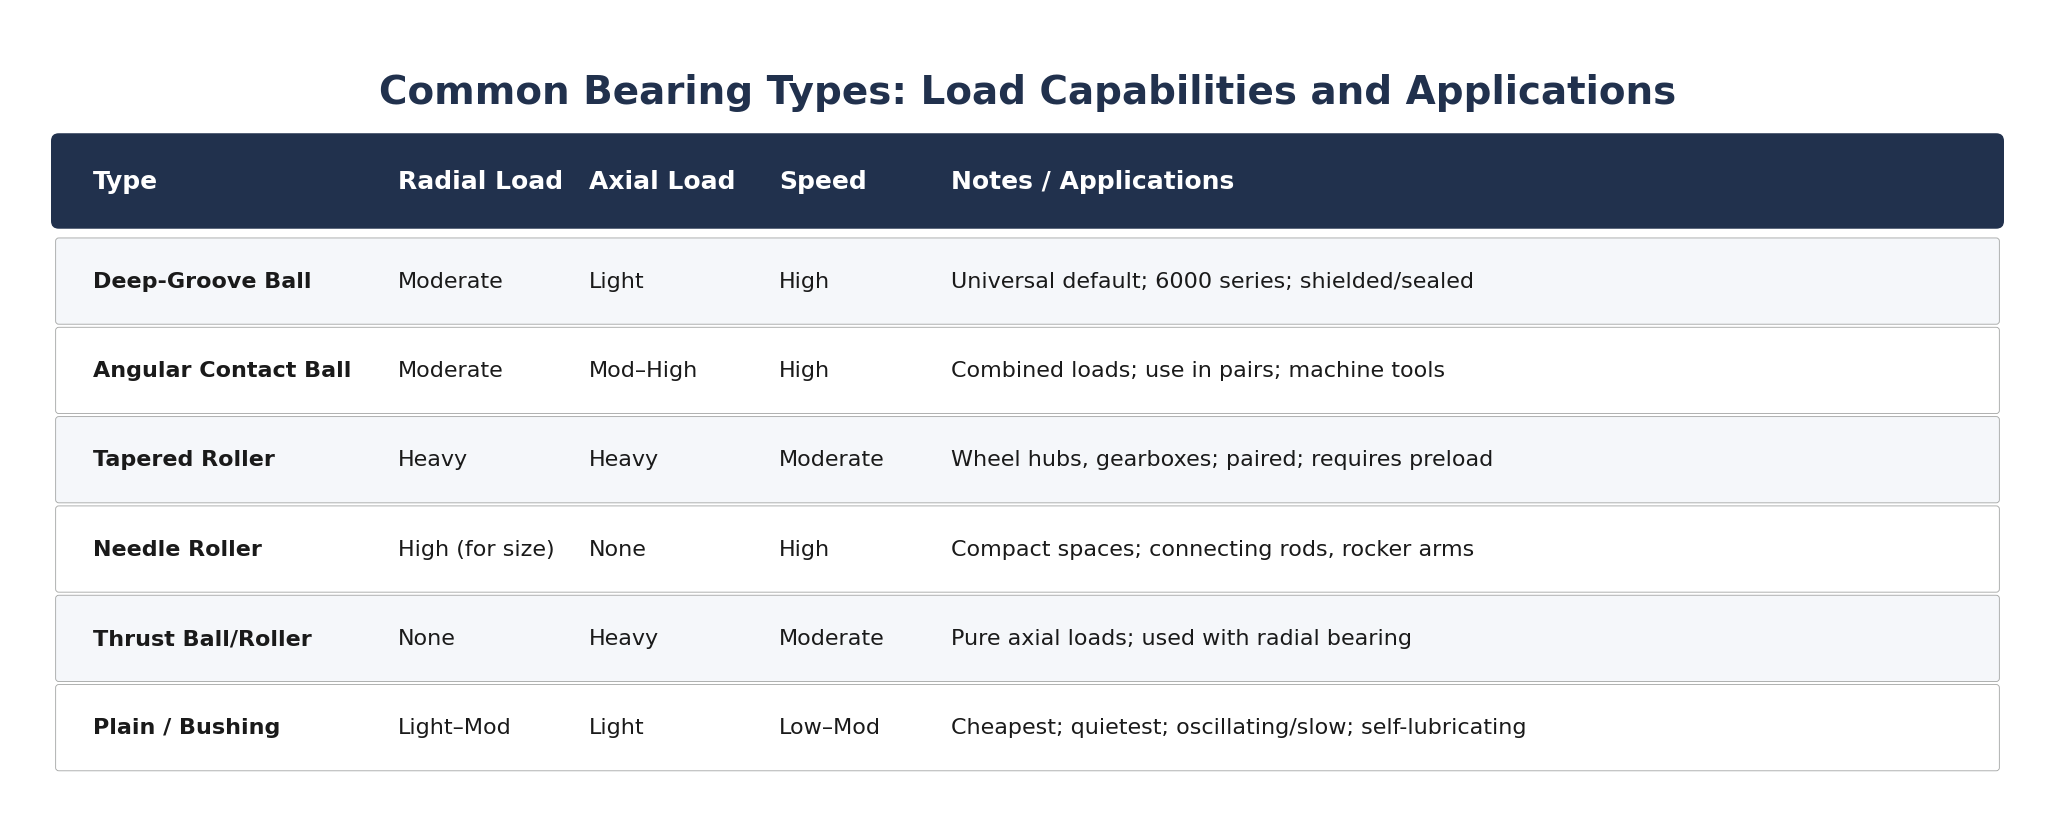
\includegraphics[width=\textwidth]{Mechanical Fasteners and Bearings/fig_bearing_types.png}
\caption{Common bearing types with load capabilities, speed ratings, and typical applications.}\label{fig:bearings}
\end{figure}

\textbf{Deep-groove ball bearings}: The universal default. Handle moderate radial and light axial loads. High speed capability. Low friction. Available in every size from 1\,mm bore to 300\,mm+. Shielded (ZZ) or sealed (2RS) variants include integral grease retention. Use these unless you have a specific reason not to.

\textbf{Angular contact ball bearings}: Handle combined radial and axial loads. The contact angle (typically 15\ensuremath{{}^{\circ}}, 25\ensuremath{{}^{\circ}}, or 40\ensuremath{{}^{\circ}}) determines the axial-to-radial load ratio. Must be used in pairs (back-to-back or face-to-face) to handle axial loads in both directions. Common in machine tool spindles.

\textbf{Tapered roller bearings}: Handle heavy combined radial and axial loads. Used in wheel hubs, gearboxes, and heavy machinery. Always used in pairs. Require careful preload adjustment.

\textbf{Needle roller bearings}: Very thin cross-section for applications where radial space is limited. High radial load capacity for their size. Cannot handle axial loads. Used in connecting rods, rocker arms, and compact gearboxes.

\textbf{Thrust bearings} (ball or roller): Handle pure axial loads. Cannot handle radial loads. Used in conjunction with a radial bearing when axial loads must be carried separately.

\textbf{Plain bearings} (bushings, journal bearings): A simple sleeve (bronze, PTFE-lined, polymer) that supports a rotating shaft. Lower speed and load capacity than rolling-element bearings, but much cheaper, quieter, and more compact. Excellent for oscillating or slow-rotation applications. Self-lubricating polymer bushings (Igus iglide) are ideal for student projects.

\subsection{Bearing Selection}

\begin{figure}[ht!]\centering
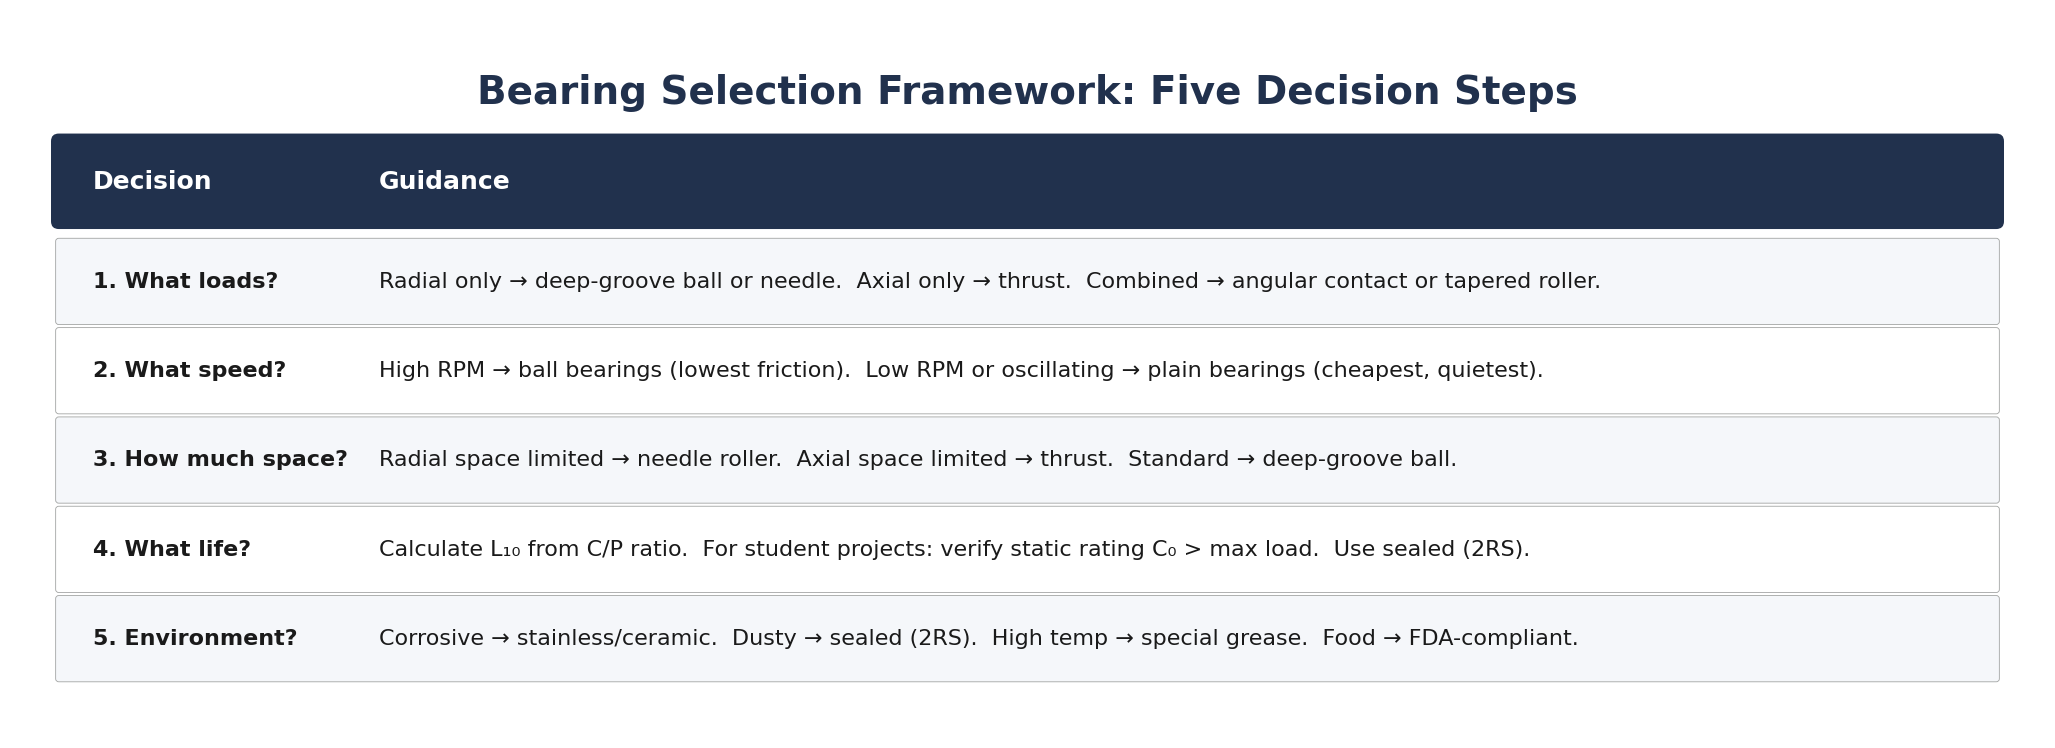
\includegraphics[width=\textwidth]{Mechanical Fasteners and Bearings/fig_bearing_selection.png}
\caption{Bearing selection framework: load type, speed, space, and life requirements drive the choice.}\label{fig:bearsel}
\end{figure}

Selection starts with four questions: (1)~What loads must the bearing carry? (radial, axial, or combined --- and how heavy?), (2)~What speed will the shaft rotate at? (RPM determines the speed rating requirement), (3)~How much space is available? (bore diameter, outer diameter, and width constraints), (4)~What life is required? (hours of operation at the design load).

\textbf{Bearing life} is predicted using the basic dynamic load rating $C$ (from the manufacturer's catalog) and the equivalent dynamic load $P$:
\begin{equation}
L_{10} = \left(\frac{C}{P}\right)^3 \times 10^6 \text{ revolutions (for ball bearings)}
\end{equation}
$L_{10}$ is the life at which 10\% of a population of identical bearings will have failed. For roller bearings, the exponent is 10/3 instead of 3. Convert revolutions to hours: $L_{10h} = L_{10} / (60 \times n)$ where $n$ is RPM.

\needspace{4\baselineskip}
\begin{tipbox}[Bearing Sizing for Student Projects]
For most MEGN~301 projects, bearing life calculation is overkill --- your prototype will operate for tens of hours, not thousands. Instead, focus on: (1)~correct bore size to match your shaft, (2)~adequate static load rating $C_0$ to handle your maximum load without permanent deformation (brinelling), and (3)~sealed or shielded variants to avoid the need for external lubrication systems. Deep-groove ball bearings (6000 series) with 2RS seals are the default choice.
\end{tipbox}

\subsection{Bearing Mounting}
Bearings require proper fits on both the shaft and in the housing to function correctly. The shaft fit is typically a light interference fit (k5 or k6) so the inner ring rotates with the shaft without slipping. The housing fit is typically a sliding fit (H7) so the outer ring can be pressed into the housing but does not spin.

\textbf{Axial retention}: Bearings must be constrained axially. Common methods: shoulder on shaft + retaining ring, shoulder + lock nut, press fit into a blind bore, or snap ring in housing groove. Always constrain at least one ring axially.

\textbf{Preload}: For precision applications (machine tools, spindles), bearing pairs are preloaded to eliminate internal clearance, increase stiffness, and improve accuracy. For student projects, standard clearance (C0 or CN) is adequate.

\needspace{4\baselineskip}
\begin{tipbox}[Mounting Bearings in 3D Prints]
Standard bearing fits (H7 housing, k6 shaft) assume machined metal with tolerances of $\pm 0.01$\,mm. FDM and resin printers cannot reliably achieve this --- typical FDM tolerances are $\pm 0.2$\,mm. If you CAD an H7 bore and print it in PLA, the bearing will either rattle loosely or crack the plastic when press-fit. Three practical solutions for 3D-printed bearing housings: (1)~Design \textbf{crush ribs}---three or four small radial ribs inside the bore that deform when the bearing is pressed in, providing a snug fit without requiring precise bore diameter. (2)~Design the bore \textbf{line-to-line} (nominal bearing OD) and secure the outer ring with \textbf{retaining compound} (Loctite 609 or 638). (3)~Print the bore 0.1--0.2\,mm undersize and \textbf{ream to final dimension} with a hand reamer. Option~1 is the simplest and most forgiving for student projects.
\end{tipbox}

\subsection{Fastener and Bearing Failure Modes}

\begin{table}[ht!]
\centering\small
\begin{tabularx}{\textwidth}{l l X X}
\toprule
\textbf{Component} & \textbf{Failure Mode} & \textbf{Root Cause} & \textbf{Prevention} \\
\midrule
Bolt & Fatigue fracture & Cyclic loading above endurance limit & Adequate preload; rolled threads; avoid stress risers \\
Bolt & Vibration loosening & Transverse vibration overcomes friction & Nyloc nut, threadlocker, or Nord-Lock washers \\
Bolt & Hydrogen embrittlement & High-strength steel + hydrogen source & Avoid Grade~8/Class~10.9+ in corrosive or plated applications without baking \\
Bolt & Stripping & Over-torque or insufficient engagement & Min 1.5$\times$ diameter thread engagement; use torque wrench \\
Bearing & Fatigue spalling & Normal wear; rolling contact fatigue & Design for adequate $L_{10}$ life \\
Bearing & Brinelling & Static overload; impact; improper mounting & Verify static load rating $C_0$; never hammer bearings \\
Bearing & Contamination & Dirt, water, or debris entry & Use sealed (2RS) bearings; proper housing seals \\
Bearing & Misalignment & Shaft/housing not coaxial & Self-aligning bearings or precision machining \\
Bearing & Lubrication failure & Grease breakdown or depletion & Sealed bearings for student projects; relubrication schedule for production \\
Bolt & Galvanic corrosion & Dissimilar metals + electrolyte (moisture) & Use compatible metals; dielectric grease; insulating washers \\
\bottomrule
\end{tabularx}
\caption{Common fastener and bearing failure modes with prevention strategies.}
\end{table}

\needspace{4\baselineskip}
\begin{warningbox}[Never Hammer a Bearing]
Mounting bearings by striking them with a hammer transmits impact loads through the rolling elements, creating permanent dents (brinelling) in the raceways. These dents cause vibration, noise, and premature failure from the moment the system first turns. Use a bearing press or a properly sized mounting tube that contacts only the ring being fitted. If mounting the inner ring onto a shaft, the force must pass through the inner ring --- never through the outer ring and balls.
\end{warningbox}

\FloatBarrier
\section{Design Rules of Thumb}

\begin{enumerate}[leftmargin=1.5em]
\item \textbf{Thread engagement}: minimum 1.5$\times$ bolt diameter in steel, 2.0$\times$ in aluminum, 2.5$\times$ in plastic. Less engagement = stripped threads under load.
\item \textbf{Bolt spacing}: minimum 3$\times$ bolt diameter center-to-center; minimum 1.5$\times$ diameter from bolt center to edge. Closer spacing risks tear-out.
\item \textbf{Bolt patterns}: Use at least 3 bolts for a bolted joint (2 for shear alignment, 3+ for moment resistance). Distribute bolts symmetrically around the load path.
\item \textbf{Bearing shaft fits}: Rotating inner ring = interference fit (k5/k6). Stationary inner ring = sliding fit (h6/g6). Housing: stationary outer ring = interference (M7/N7). Rotating outer ring = sliding (H7).
\item \textbf{Shaft shoulders}: Provide a shoulder for axial location. Shoulder height $\geq$ bearing fillet radius (check catalog). Undercut or relief groove if the shoulder radius is too large.
\item \textbf{Heat-set inserts}: For threaded connections into 3D-printed or injection-molded plastic, use brass heat-set inserts rather than tapping threads directly into the plastic. The insert provides a metal-to-metal thread engagement that does not strip, degrade with thermal cycling, or creep under sustained load.
\end{enumerate}

\FloatBarrier
\section{Practice Questions}
Questions are tiered: \textbf{C} = Comprehension, \textbf{A} = Application, \textbf{CT} = Critical Thinking.
\begin{enumerate}[leftmargin=1.5em]
\item \textbf{[C]} Explain the difference between a bolt and a screw. When would you choose one over the other?
\item \textbf{[C]} What do the numbers in ``Class 8.8'' mean? Calculate the ultimate tensile strength and yield strength.
\item \textbf{[A]} A joint requires 5\,kN of clamping force using an M8 bolt. The nut factor is $K = 0.20$. Calculate the required torque. If the bolt is Class~8.8, is this within the proof load?
\item \textbf{[A]} Your motor mount experiences significant vibration. The mount uses four M5 bolts. Specify an appropriate locking method and justify your choice.
\item \textbf{[A]} Select a bearing for a shaft that rotates at 1500\,RPM under a 200\,N radial load and 50\,N axial load. The shaft is 10\,mm diameter. Justify your bearing type selection and specify a part number from a standard catalog.
\item \textbf{[CT]} Your teammate's design uses M3 screws threaded directly into a PLA 3D-printed bracket to mount a motor that produces 0.4\,Nm of torque. Identify every failure mode and propose a redesign using appropriate fastening methods.
\item \textbf{[CT]} A bearing in your system is making a grinding noise after 20 hours of operation. The bearing is a deep-groove ball bearing, 6001-2RS. Walk through a systematic diagnosis: what are the possible causes and how would you investigate each?
\end{enumerate}

\subsection{Answers}
\begin{enumerate}[leftmargin=1.5em]
\item A bolt passes through clearance holes in both parts and is secured by a nut; a screw threads into a tapped hole in one part. Use a bolt when: you need to clamp thick stacks, you want to access the joint from one side with a wrench, or you need the nut as a locking device (Nyloc). Use a screw when: you cannot access the back side, the mating part is thick enough for adequate thread engagement, or you need a flush surface (countersunk screw).

\item Class 8.8: first digit $\times$ 100 = UTS = 800\,MPa. First $\times$ second $\times$ 10 = yield = 640\,MPa. Proof load $\approx$ 580\,MPa (90\% of yield).

\item $T = K \cdot F_i \cdot d = 0.20 \times 5000\,\text{N} \times 0.008\,\text{m} = 8.0$\,Nm. M8 Class~8.8 proof load: stress area $= 36.6$\,mm$^2$, proof stress $= 580$\,MPa, $F_{\text{proof}} = 36.6 \times 580 = 21.2$\,kN. 5\,kN preload is 23.6\% of proof load --- well within the safe range (target 60--75\%).

\item Nyloc lock nut is the best choice: effective against vibration loosening, easy to install, low cost, and readily available in M5. Thread-locking adhesive (Loctite 242 blue) is a good alternative if you need to reuse the bolts. Split lock washers are the weakest option and are not recommended for vibration-critical joints. Specify: ``M5$\times$0.8$\times$16, Class~8.8, with M5 Nyloc nut, torque to 5.5\,Nm.''

\item Load: 200\,N radial + 50\,N axial. This is a combined load that a deep-groove ball bearing handles well. For 10\,mm bore: 6000-2RS (OD 26\,mm, width 8\,mm, $C = 4.75$\,kN, $C_0 = 1.96$\,kN). Equivalent dynamic load $P = F_r + Y \cdot F_a \approx 200 + 1.5 \times 50 = 275$\,N. $L_{10} = (4750/275)^3 = 5151 \times 10^6$ rev $= 57{,}200$ hours at 1500\,RPM. Far more than adequate. The 2RS seal provides lifetime lubrication.

\item Failure modes: (a) PLA threads strip under sustained torque --- PLA creeps under load and has very low shear strength in layer-line direction. (b) Motor vibration loosens M3 screws --- no locking method specified. (c) PLA softens above 60\degC{} --- motor heat may reach this. Redesign: (a) Install M3 brass heat-set inserts into the PLA bracket. (b) Use M3 Class~8.8 socket head cap screws with Loctite 242. (c) Increase bracket wall thickness around inserts to 2$\times$ insert OD. (d) Add locating features (dowel pins or alignment boss) so the bolt pattern does not carry the full shear load.

\item Systematic diagnosis: (1) Contamination --- most common cause. Even sealed bearings can ingest debris during improper mounting. Inspect for visible contamination by removing the bearing and checking for gritty feel when rotated by hand. (2) Brinelling --- check for evenly spaced dents from impact during mounting (hammering). Rotate slowly by hand and feel for periodic ``bumps.'' (3) Misalignment --- check shaft and housing concentricity with a dial indicator. Misalignment causes uneven loading and heat. (4) Lubrication failure --- sealed bearings should not need relubrication at 20 hours; if the seal was damaged during mounting, grease may have escaped. (5) Overload --- verify actual loads against the bearing rating. Resolution: replace the bearing (bearings are consumables, not repairable), correct the root cause before installing the replacement, and use proper mounting techniques (press, not hammer).
\end{enumerate}

\needspace{4\baselineskip}
\begin{tipbox}[Industry SE Parallels]
Fastener and bearing specifications appear in multiple SE artifacts: the BOM (part numbers, grades, quantities), engineering drawings (torque callouts, fit tolerances), ICDs (mounting interface definitions), maintenance manuals (torque re-check schedules, bearing replacement intervals), and the FMECA (fastener loosening and bearing failure as identified failure modes). Fastener torque verification is a common inspection-method (I) requirement in the VCRM.
\end{tipbox}



\FloatBarrier
\chapter{Mechanical Power Transmission}

\vspace{1em}

\begin{keyconceptbox}[Bottom Line]
Power transmission converts the torque and speed at a motor shaft into the force and velocity your mechanism needs. Every transmission element---belt, chain, gear, shaft, linkage, or lead screw---trades speed for torque (or vice versa), and every one introduces losses. Selecting the right transmission and sizing it correctly is the bridge between your electrical power budget (Chapter~8) and the mechanical work your system must perform.
\end{keyconceptbox}

\vspace{1em}

\FloatBarrier
\section{Fundamental Relationships}

All mechanical power transmission obeys a small set of relationships. \textbf{Power} is conserved (minus losses):
\begin{equation}
P = T \cdot \omega = F \cdot v
\end{equation}
where $T$ is torque (Nm), $\omega$ is angular velocity (rad/s), $F$ is linear force (N), and $v$ is linear velocity (m/s). The \textbf{gear ratio} (or transmission ratio) $i$ relates input and output:
\begin{equation}
i = \frac{\omega_{\text{in}}}{\omega_{\text{out}}} = \frac{T_{\text{out}}}{T_{\text{in}} \cdot \eta} = \frac{N_{\text{driven}}}{N_{\text{driver}}}
\end{equation}
where $\eta$ is the efficiency of the transmission stage and $N$ is the number of teeth (gears), grooves (pulleys), or teeth (sprockets). A ratio $i > 1$ is a speed reduction (torque multiplication); $i < 1$ is a speed increase (torque reduction). Most mechanisms need speed reduction because motors spin fast ($\sim$1000--10{,}000\,RPM) but mechanisms need slow, forceful motion.

\textbf{Efficiency} is always less than 100\%. Each transmission stage introduces losses from friction, windage, and deformation. Losses compound multiplicatively: three stages at 95\% each yield $0.95^3 = 85.7\%$ overall. Minimize the number of stages.

\FloatBarrier
\section{Belt and Pulley Drives}

\begin{figure}[ht!]\centering
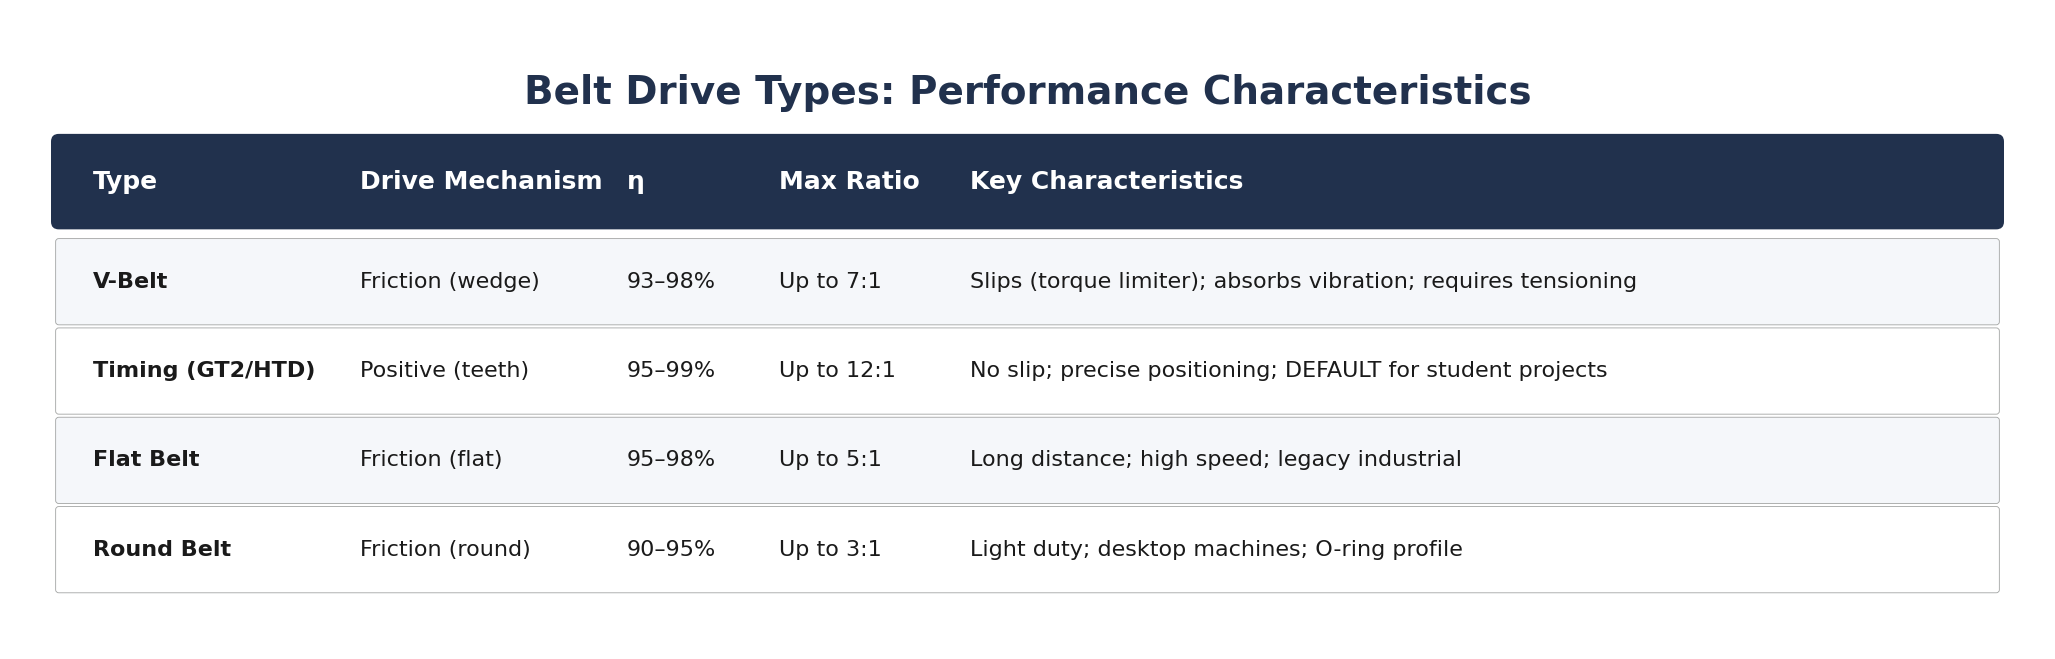
\includegraphics[width=\textwidth]{Mechanical Power Transmission/fig_belt_types.png}
\caption{Belt drive types: V-belt, timing (synchronous), flat, and round with performance characteristics.}\label{fig:belts}
\end{figure}

\subsection{V-Belts}
Wedge-shaped cross-section grips the pulley groove through friction. Absorbs shock and vibration. Slips under overload (acts as a torque limiter, which can be a safety feature). Efficiency: 93--98\%. Speed ratio limited to about 7:1 per stage. Tension must be maintained --- belts stretch over time and require periodic re-tensioning. Common in HVAC, compressors, and automotive accessories.

\subsection{Timing Belts (Synchronous)}
Toothed belt meshes with toothed pulleys. \textbf{No slip} --- positive engagement means precise speed ratio and position control. Efficiency: 95--99\%. Quiet operation. No re-tensioning needed (teeth prevent slip). Used in 3D printers, CNC machines, robotics, and automotive camshaft drives. \textbf{This is the default choice for student projects requiring linear or rotary positioning.}

\needspace{4\baselineskip}
\begin{tipbox}[GT2 Timing Belts for Student Projects]
The GT2 profile (2\,mm pitch) is the standard for hobby and prototyping applications. Belt widths of 6\,mm or 10\,mm are common. GT2 pulleys are available in 16, 20, 36, and 60 tooth variants for standard NEMA~17 motor shafts (5\,mm bore). A 20T driving a 60T pulley gives a 3:1 reduction. GT2 belt, pulleys, and idlers are inexpensive (\$5--15 per axis) and available from Amazon, Aliexpress, and robotics suppliers.
\end{tipbox}

\needspace{4\baselineskip}
\begin{tipbox}[MEGN 301 in Practice: Power Transmission Sourcing]
Common sources for student projects: \textbf{ServoCity / Actobotics} (gears, hubs, shafts, couplings with matching mounting patterns), \textbf{Pololu} (gearmotors with integrated gearboxes, timing belts, linear actuators), \textbf{SDP/SI} (stock metric and imperial spur gears, timing pulleys, precision shafts), \textbf{McMaster-Carr} (everything, premium price, fast), \textbf{Amazon} (GT2 belt kits, planetary gearboxes for NEMA~17, couplings). A complete GT2 linear axis kit (belt, pulleys, linear rail, carriage, motor mount) is available for \$15--25 and provides an instant X or Y axis for your project.
\end{tipbox}

\subsection{Flat and Round Belts}
Flat belts are used for long-distance power transmission (lathe line shafts, conveyor systems). Round belts (O-ring style) are used for light-duty applications like desktop machines. Neither is common in student projects.

\FloatBarrier
\section{Chain Drives}

\textbf{Roller chain} (bicycle chain, ANSI standard) provides positive engagement like timing belts but handles much higher loads. Standard sizes: \#25 (1/4\,in pitch), \#35 (3/8\,in), \#40 (1/2\,in), \#50 (5/8\,in). Efficiency: 95--98\%. Requires lubrication. Noisy at high speed. Used when loads exceed belt capacity or in dirty/oily environments where belts would degrade.

\textbf{Selection}: Match chain pitch to load. \#25 chain handles about 100\,lbs working load; \#35 handles 250\,lbs; \#40 handles 500\,lbs. Sprocket tooth count: minimum 17 teeth on the driver to avoid ``chordal action'' (speed pulsation). Speed ratio up to 7:1 per stage.

\needspace{4\baselineskip}
\begin{warningbox}[Chain Requires Lubrication and Tensioning]
An unlubricated chain wears rapidly --- the pins and bushings lose material, the chain ``stretches'' (actually elongates from wear), and eventually jumps teeth or breaks. For student projects, apply chain lubricant (or light oil) before every test session. Chain tension must be adjustable --- include a slot or adjustable mount for the driven sprocket.
\end{warningbox}

\FloatBarrier
\section{Gear Trains}

\begin{figure}[ht!]\centering
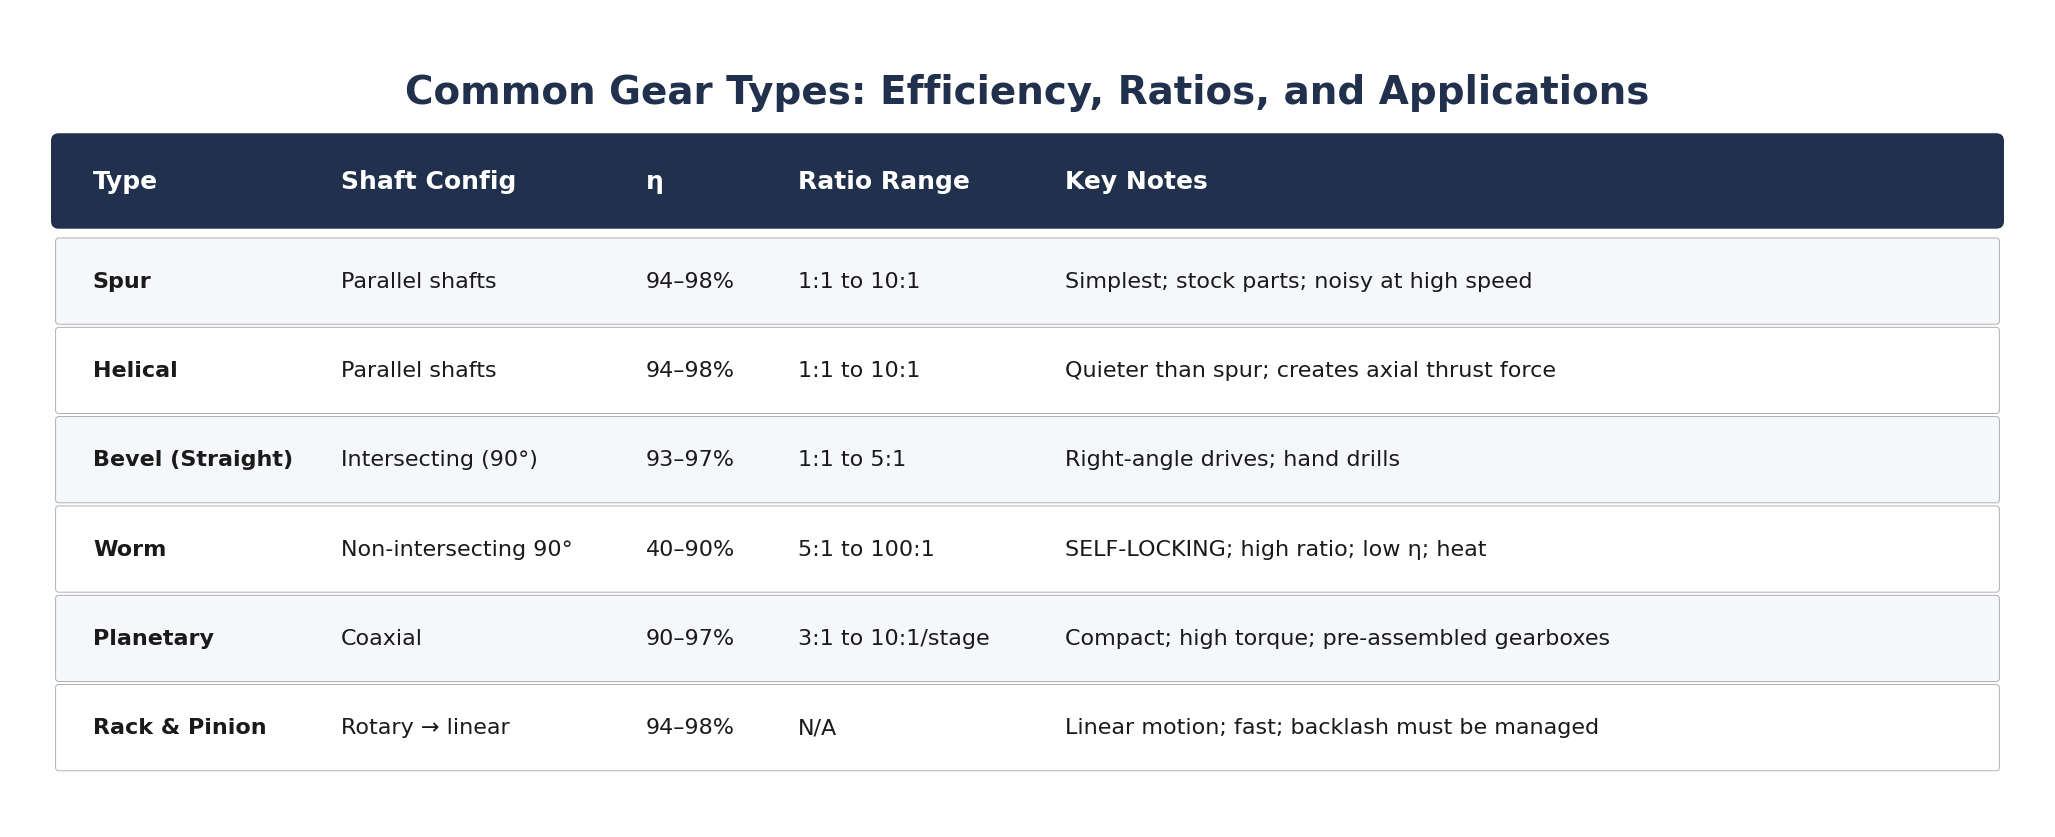
\includegraphics[width=\textwidth]{Mechanical Power Transmission/fig_gear_types.png}
\caption{Common gear types with efficiency, ratio range, and typical applications.}\label{fig:gears}
\end{figure}

\subsection{Spur Gears}
Straight teeth parallel to the shaft axis. The simplest and most common gear type. Mesh on parallel shafts. Efficiency: 94--98\% per mesh. Noisy at high speed because the entire tooth face engages and disengages simultaneously. Available as stock components in standard modules (metric) or diametral pitches (imperial) from suppliers like SDP/SI, McMaster-Carr, and ServoCity.

\subsection{Helical Gears}
Teeth cut at an angle to the shaft axis. Quieter and smoother than spur gears because engagement is gradual. However, the helix angle produces an axial (thrust) force that must be supported by the shaft bearings. Efficiency: 94--98\%.

\subsection{Bevel Gears}
Transmit motion between intersecting shafts (typically 90\ensuremath{{}^{\circ}}). Straight bevel gears are the simplest; spiral bevel gears are quieter and handle higher loads. Common in hand drills, differential gears, and right-angle drives.

\subsection{Worm Gears}
A worm (helical screw) meshes with a worm wheel. Very high ratios in a single stage (5:1 to 100:1). The key advantage: many worm gear sets are \textbf{self-locking} --- the load cannot back-drive the motor. This is critical for applications like hoists, jacks, and positioning stages where the mechanism must hold position without power. Efficiency: 40--90\% (lower than other gear types due to sliding contact). The self-locking property exists when the lead angle is below the friction angle (typically below $\sim$6\ensuremath{{}^{\circ}}).

\subsection{Planetary (Epicyclic) Gears}
A sun gear, planet gears, and a ring gear in a compact coaxial arrangement. High torque density --- very high ratios (3:1 to 10:1 per stage) in a small package. Coaxial input and output (the shaft stays on the same axis). Used in cordless drills, robotic joints, and automotive transmissions. Pre-assembled planetary gearboxes for NEMA~17 and NEMA~23 motors are available for \$20--80 and are the easiest way to add gear reduction to a stepper or DC motor in a student project.

\needspace{4\baselineskip}
\begin{tipbox}[Gear Selection for Student Projects]
For most MEGN~301 projects, you have three practical options: (1)~A pre-assembled \textbf{planetary gearbox} that bolts directly to your motor. Easiest integration; highest cost (\$25--80). (2)~\textbf{Spur gears} from a robotics supplier (ServoCity, Actobotics) with matching hubs and shafts. Most flexible; moderate cost and effort. (3)~\textbf{3D-printed gears} for low-load, low-speed applications. Cheapest but lowest strength and precision; use herringbone profile to eliminate axial thrust and improve meshing.

\textbf{Quick Decision Tree:}
\begin{itemize}[nosep]
\item Need to hold position without power? $\to$ \textbf{Worm gear} (self-locking) or \textbf{lead screw}.
\item Need precise linear positioning? $\to$ \textbf{Lead screw} + stepper motor.
\item Need fast linear motion? $\to$ \textbf{GT2 belt-driven stage} on linear rails.
\item Need speed reduction, parallel shafts? $\to$ \textbf{Planetary gearbox} or \textbf{timing belt}.
\item Need right-angle drive? $\to$ \textbf{Bevel gears} or \textbf{worm gear}.
\item Need shock absorption? $\to$ \textbf{V-belt} or \textbf{flexible coupling}.
\end{itemize}
\end{tipbox}

\FloatBarrier
\section{Shafts and Couplings}

\subsection{Shaft Design}
Shafts transmit torque and support rotating components. Key design parameters: \textbf{diameter} (sized for torque via $\tau = T \cdot c / J$ and deflection), \textbf{material} (1045 steel for general purpose; 4140 for high strength; 303/304 stainless for corrosion resistance; aluminum 6061-T6 for light weight), \textbf{keyways} (transmit torque from shaft to hub via a rectangular key), and \textbf{surface finish} (bearing journals require ground finish, Ra $\leq$ 0.4\,$\mu$m).

\subsection{Shaft-Hub Connections}
\textbf{Set screws}: Simplest; a screw in the hub bears against the shaft (or a flat machined on the shaft). Adequate for light loads but slips under high torque. Two set screws at 90\ensuremath{{}^{\circ}}{} are better than one.

\textbf{Keyways}: A rectangular key in matching slots in shaft and hub transmits torque positively. Standard key sizes are tabulated by shaft diameter (Machinery's Handbook). Most reliable for moderate-to-high torque. Requires milling a keyway in both shaft and hub.

\textbf{Clamping hubs}: A split hub that clamps concentrically around the shaft via bolts. No keyway needed; provides zero-backlash torque transmission. Common in robotics (ServoCity clamp hubs).

\textbf{Press fits}: Interference fit between shaft and bore. Zero backlash, highest torque capacity, but permanent (requires a press to assemble and disassemble). Used in production; rare in student prototypes.

\subsection{Shaft Couplings}
Couplings connect two shafts end-to-end. Types ranked by misalignment tolerance:

\textbf{Rigid couplings}: Zero misalignment tolerance. Both shafts must be perfectly coaxial. Simple and stiff but unforgiving.

\textbf{Flexible jaw couplings} (Lovejoy, spider coupling): Accommodate up to 1\ensuremath{{}^{\circ}}{} angular and 0.5\,mm parallel misalignment. The elastomer spider absorbs shock and vibration. Good default choice for motor-to-gearbox connections in student projects.

\textbf{Beam couplings} (helical couplings): A single piece of aluminum with helical cuts. Very flexible in angular, parallel, and axial misalignment. Zero backlash. Common in precision positioning systems (CNC, 3D printers). Fragile under high torque.

\textbf{Oldham couplings}: Handle large parallel misalignment but zero angular misalignment. Used when shafts are parallel but offset.

\textbf{Universal joints} (U-joints, Cardan joints): Handle large angular misalignment (up to 45\ensuremath{{}^{\circ}}). Non-constant velocity at a single joint; use in pairs to cancel the velocity variation. Used in automotive driveshafts.

\FloatBarrier
\section{Linear Motion Systems}

\begin{figure}[ht!]\centering
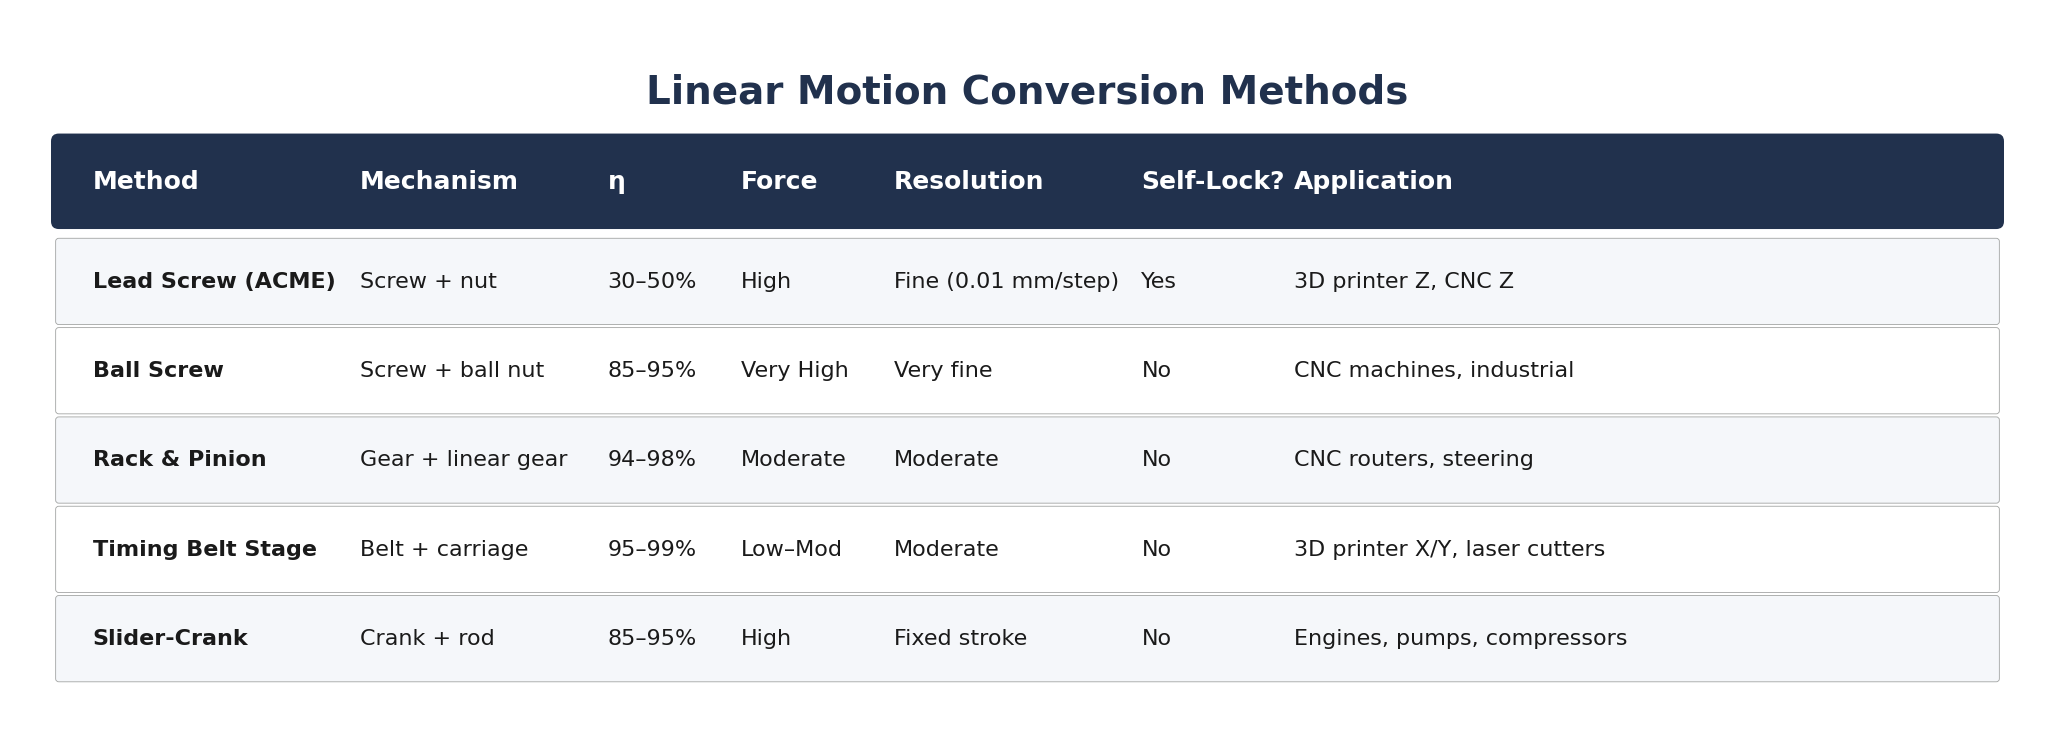
\includegraphics[width=\textwidth]{Mechanical Power Transmission/fig_linear_motion.png}
\caption{Linear motion conversion methods: lead screw, ball screw, rack and pinion, belt drive, and linkage.}\label{fig:linear}
\end{figure}

\subsection{Lead Screws}
A threaded rod (lead screw) turns inside a nut, converting rotary motion to linear motion. The \textbf{lead} is the linear distance the nut travels per revolution of the screw. A 2\,mm lead screw advances 2\,mm per turn; at 200 steps/rev (stepper motor), resolution is 0.01\,mm/step. Advantages: high force, fine resolution, self-locking (cannot be back-driven). Disadvantages: friction limits speed and efficiency ($\sim$30--50\% for ACME threads). Used in 3D printers (Z-axis), CNC machines, and positioning stages.

\subsection{Ball Screws}
Like a lead screw but with recirculating ball bearings between the screw and nut, dramatically reducing friction. Efficiency: 85--95\%. Higher speed capability. \textbf{Not self-locking} --- the load can back-drive the motor (requires a brake or motor holding torque). More expensive than lead screws. Used in CNC machines, industrial automation, and precision stages.

\subsection{Rack and Pinion}
A spur gear (pinion) meshes with a linear gear (rack), converting rotary to linear motion. Linear speed = $\pi \cdot d \cdot n$ where $d$ is the pinion pitch diameter and $n$ is RPM. Bidirectional, fast, and capable of long travel distances. Backlash is inherent and must be managed (spring-loaded split pinion or anti-backlash rack). Used in CNC routers, camera sliders, and steering systems.

\subsection{Belt-Driven Linear Stages}
A GT2 timing belt in a closed loop, with one span attached to a carriage running on linear rails. The motor turns a pulley; the belt moves the carriage linearly. Fast, quiet, lightweight, and the most common linear drive in 3D printers (X and Y axes) and desktop CNC machines. No self-locking. Load capacity limited by belt tension.

\FloatBarrier
\section{Linkages}

\subsection{Four-Bar Linkages}
The most fundamental planar mechanism: four rigid links connected by four revolute (pin) joints. By varying the link lengths, a four-bar linkage can produce: \textbf{crank-rocker} (one link rotates fully, the other oscillates), \textbf{double-crank} (both input and output rotate fully), or \textbf{double-rocker} (both oscillate). Grashof's criterion: the linkage has at least one full-rotating link if $s + l \leq p + q$ where $s$ is the shortest link, $l$ is the longest, and $p$, $q$ are the others.

\subsection{Slider-Crank Mechanisms}
Converts rotary motion to reciprocating linear motion (or vice versa). The connecting rod links a rotating crank to a slider in a linear guide. This is the mechanism inside every piston engine, reciprocating compressor, and many packaging machines. Stroke = $2 \times$ crank radius.

\subsection{Cam-Follower Mechanisms}
A cam (a shaped rotating profile) drives a follower (a lever or slider) through a prescribed motion profile. The cam profile is designed to produce specific displacement, velocity, and acceleration characteristics. Used in engine valve trains, automated assembly, and packaging machines. Not common in student projects but important to recognize.

\FloatBarrier
\section{Selection Framework}

\begin{figure}[ht!]\centering
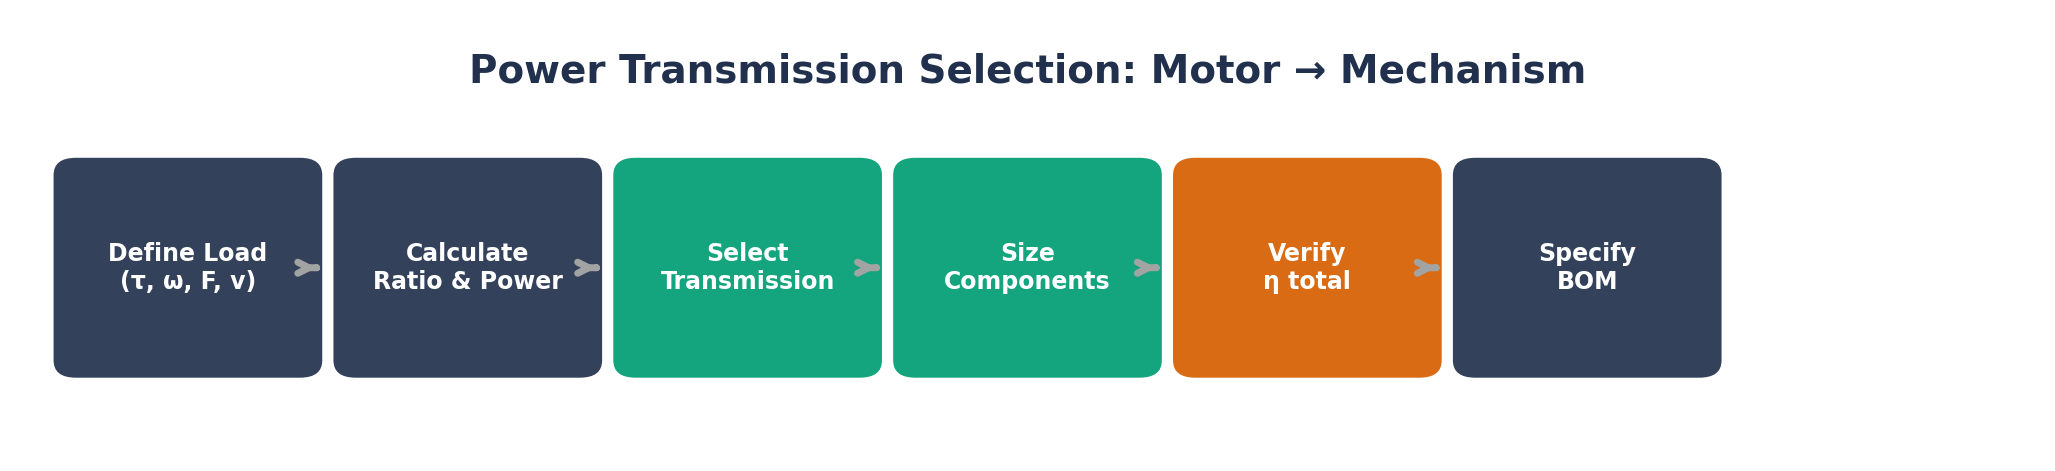
\includegraphics[width=\textwidth]{Mechanical Power Transmission/fig_transmission_selection.png}
\caption{Power transmission selection framework: rotary-to-rotary, rotary-to-linear, and direct drive options.}\label{fig:transselect}
\end{figure}

\begin{center}
\small
\begin{tabularx}{\textwidth}{l X l l}
\toprule
\textbf{Need} & \textbf{Best Options} & \textbf{Efficiency} & \textbf{Self-Locking?} \\
\midrule
Speed reduction, parallel shafts & Timing belt, spur gears, planetary gearbox & 90--98\% & No \\
Speed reduction, right angle & Bevel gears, worm gear & 40--98\% & Worm: yes \\
High ratio, compact & Planetary gearbox, worm gear & 40--97\% & Worm: yes \\
Precise linear positioning & Lead screw + stepper, ball screw & 30--95\% & Lead screw: yes \\
Fast linear motion & Belt-driven stage, rack \& pinion & 90--98\% & No \\
Reciprocating motion & Slider-crank, scotch yoke, cam & 85--95\% & No \\
Hold position without power & Worm gear, lead screw & 30--70\% & Yes \\
Absorb shock/misalignment & V-belt, flexible coupling, chain & 90--98\% & No \\
\bottomrule
\end{tabularx}
\end{center}

\FloatBarrier
\section{Practice Questions}
Questions are tiered: \textbf{C} = Comprehension, \textbf{A} = Application, \textbf{CT} = Critical Thinking.
\begin{enumerate}[leftmargin=1.5em]
\item \textbf{[C]} Explain the difference between a timing belt and a V-belt. When would you use each?
\item \textbf{[C]} Why are worm gears self-locking? What is the disadvantage of this property?
\item \textbf{[A]} A NEMA~17 stepper motor produces 0.4\,Nm at the shaft. You need 1.5\,Nm at the output. Design a single-stage reduction using a timing belt and specify the pulley tooth counts.
\item \textbf{[A]} You are designing a linear positioning stage for the Sol-Mate Purification Pal that must travel 150\,mm with 0.1\,mm resolution. Compare a lead screw drive vs.\ a belt-driven stage. Which do you recommend and why?
\item \textbf{[A]} Your robot arm joint uses a 50:1 worm gearbox. The motor draws 2\,A at 12\,V (24\,W input). If the worm gear efficiency is 60\%, what is the mechanical output power? What happens to the other 40\%?
\item \textbf{[CT]} A 3D-printed gear in your prototype stripped after 8 hours of testing. The gear is PLA, module 1.5, 24 teeth, 6\,mm face width, transmitting 0.3\,Nm. Diagnose the failure and propose three different solutions with their tradeoffs.
\item \textbf{[CT]} You are designing the drive system for the Caffeinated Creatures coffee grinder project. The grinder burr requires 0.5\,Nm at 300\,RPM. Your motor is a 12V DC motor rated at 10{,}000\,RPM no-load and 0.02\,Nm stall torque. Design a complete power transmission from motor to burr, specifying each component.
\end{enumerate}

\subsection{Answers}
\begin{enumerate}[leftmargin=1.5em]
\item Timing belt: toothed, positive engagement, no slip, precise positioning, quieter, no re-tensioning. V-belt: friction drive, slips under overload (torque limiting), absorbs vibration, simpler pulleys, requires tensioning. Use timing belt when position accuracy matters (CNC, robotics, 3D printers). Use V-belt for general power transmission where some slip is acceptable and shock absorption is beneficial (compressors, HVAC fans).

\item Worm gears are self-locking because the high helix angle creates a friction condition where the load cannot back-drive the worm. For the gear to drive the worm, it would need to push the worm axially against friction --- and if the lead angle is below the friction angle, this is impossible. Disadvantage: the same friction that provides self-locking also means low efficiency (40--70\%). The lost energy becomes heat, which limits continuous power transmission and may require cooling.

\item Required ratio: $i = 1.5 / (0.4 \times \eta)$. With belt efficiency $\eta \approx 0.97$: $i = 1.5 / 0.388 = 3.87$, so approximately 4:1. Use a 16T driver pulley and a 60T driven pulley: ratio $= 60/16 = 3.75:1$. Output torque $= 0.4 \times 3.75 \times 0.97 = 1.46$\,Nm. Slightly below target. Options: use 15T:60T (4:1, output $= 1.55$\,Nm $\checkmark$) or add a second stage. GT2 belt, 6\,mm width, center distance calculated from pulley sizes.

\item Lead screw: 2\,mm lead with 200 step/rev stepper gives 0.01\,mm/step resolution (meets 0.1\,mm easily). Self-locking (holds position without power). Travel 150\,mm requires $\sim$200\,mm screw. Slow: at 1\,rev/s, travel speed = 2\,mm/s (75\,s for full travel). Belt drive: GT2 belt with 20T pulley (40\,mm circumference), 200 step/rev = 0.2\,mm/step. Meets 0.1\,mm with microstepping. Fast: at 5\,rev/s = 200\,mm/s (0.75\,s for full travel). Not self-locking. Recommendation: lead screw, because the application (water filter pump positioning) prioritizes precision and holding position over speed, and the self-locking property eliminates the need for a brake or continuous motor current.

\item Mechanical output: $24\,\text{W} \times 0.60 = 14.4$\,W. The other $24 - 14.4 = 9.6$\,W (40\%) is converted to heat in the worm gear mesh (friction between the worm threads and wheel teeth). This heat must be dissipated by the gearbox housing. In continuous operation, verify that the housing temperature stays within the lubricant's operating range and does not exceed safe touch temperature ($< 60$\degC\ surface).

\item PLA spur gear failure at 0.3\,Nm. Root cause: PLA has low shear strength ($\sim$35\,MPa) and poor fatigue resistance. At module 1.5, 24 teeth, 6\,mm face width, the tooth bending stress exceeds PLA's endurance limit under cyclic loading. Solutions: (a)~Reprint in Nylon-Like resin (Siraya Blu) --- 3$\times$ higher impact strength and better fatigue life, but $\sim$\$38/kg. (b)~Replace with a stock metal spur gear (McMaster or SDP/SI) --- steel or brass, indefinite life at this load, \$8--15. (c)~Increase face width to 10\,mm and switch to a herringbone tooth profile (reduces tooth stress and eliminates axial thrust) --- stays in PLA but increases part size and print time. Best option: (b) metal gear for the high-load stage, PLA only for low-load idler gears.

\item The motor produces 0.02\,Nm at stall and spins at 10,000\,RPM no-load. At the operating point ($\sim$50\% of no-load speed, $\sim$50\% of stall torque for max power), the motor delivers approximately 0.01\,Nm at 5,000\,RPM. Target: 0.5\,Nm at 300\,RPM. Required ratio: $i = 5000/300 \approx 17:1$. Required torque check: $0.01 \times 17 \times \eta = 0.01 \times 17 \times 0.85 = 0.145$\,Nm --- insufficient! The motor is too small. Solution: either (a) use a larger motor (NEMA~17 stepper at 0.4\,Nm with a 2:1 planetary reduction gives $0.4 \times 2 \times 0.9 = 0.72$\,Nm at 150\,RPM --- increase motor speed for 300\,RPM by using a 1.5:1 reduction instead), or (b) add a two-stage reduction to the existing motor --- first stage 5:1 planetary gearbox, second stage 3.4:1 timing belt, total $= 17:1$, output torque $= 0.01 \times 17 \times 0.90 \times 0.97 = 0.148$\,Nm. Still insufficient. The DC motor's torque constant is simply too low. Recommendation: replace with a 12V, 300\,RPM geared DC motor (integrated gearbox) rated for 0.5\,Nm continuous, or a NEMA~17 stepper with a 2:1 planetary gearbox.
\end{enumerate}

\needspace{4\baselineskip}
\begin{tipbox}[Industry SE Parallels]
Power transmission specifications appear in your architecture block diagram (mechanical interface between motor and load), trade studies (belt vs.\ gear vs.\ direct drive), subsystem requirements (output torque, speed, resolution, backlash tolerance), BOM (pulleys, belts, gears, bearings, couplings, shafts), ICDs (shaft diameters, key sizes, mounting bolt patterns), and maintenance plans (belt tension schedules, chain lubrication, gear oil changes). The transmission design must be verified by analysis (torque calculations, efficiency estimates) and test (output force/speed measurements under load).
\end{tipbox}


\FloatBarrier
\chapter{Designing for Injection Molding}

\vspace{1em}




\vspace{1em}


% ══════════════════════════════════════════════════════════════════════
\FloatBarrier
\section{Injection Molding Fundamentals}
% ══════════════════════════════════════════════════════════════════════

\subsection{Process Overview}

Injection molding produces plastic parts by forcing molten thermoplastic into a precision steel mold under high pressure. The machine has two units: the \textbf{injection unit} (barrel, screw, heater bands, nozzle) melts pellets and injects them, and the \textbf{clamping unit} (platens, tie bars, hydraulic or toggle mechanism) holds the mold closed. Machines are rated by clamp force (tons) and shot size (oz or g).

The mold has two halves: the \textbf{cavity} (A-side, stationary, forms the outside/cosmetic surface) and the \textbf{core} (B-side, moving, forms the inside surface). The \textbf{parting line} is where the halves meet. Inside the mold, a \textbf{runner system} distributes melt from the nozzle to the gate, \textbf{cooling channels} extract heat, and \textbf{ejector pins} push the part out.

\subsection{The Four-Phase Cycle}

\begin{figure}[ht!]
\centering
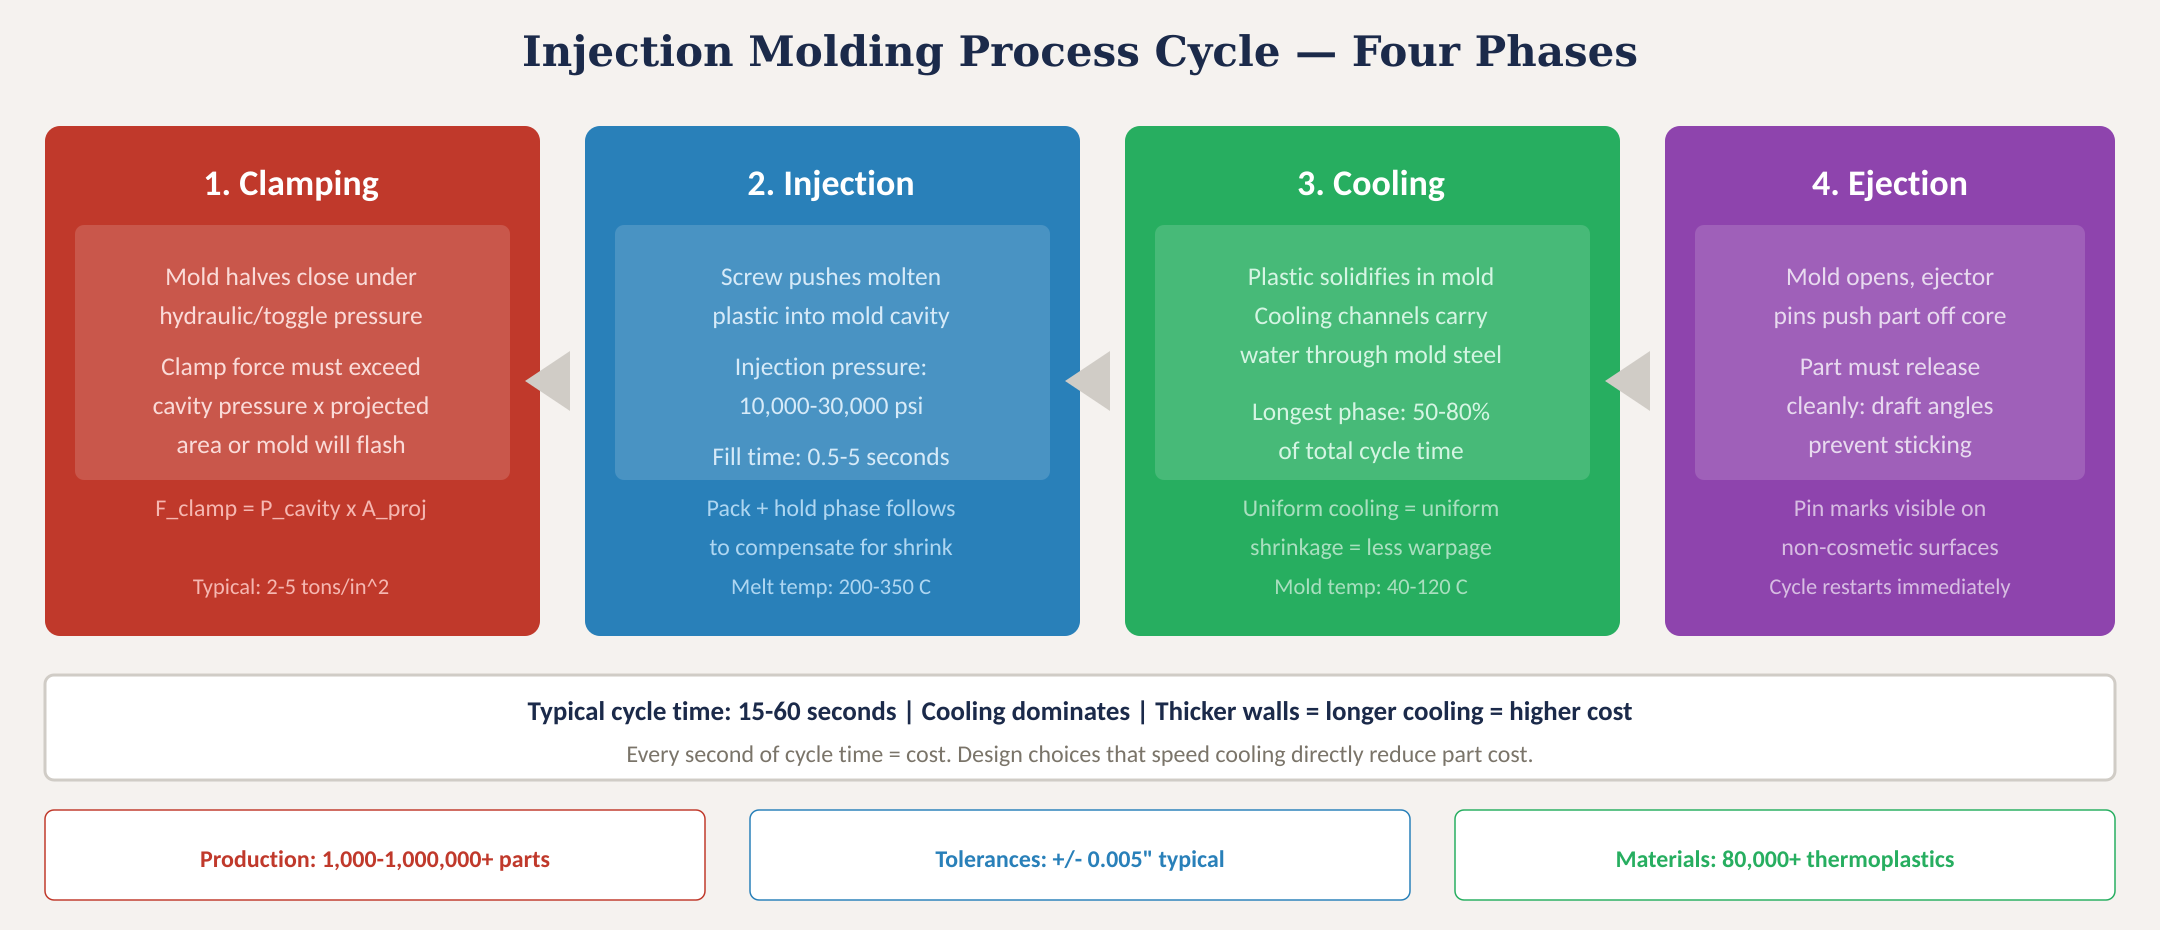
\includegraphics[width=\textwidth]{Designing for Injection Molding/fig_process_cycle.png}
\caption{Four-phase injection molding cycle with process parameters, timing, and production capabilities.}
\label{fig:cycle}
\end{figure}

\begin{enumerate}[leftmargin=1.5em]
  \item \textbf{Clamping}: Mold halves close under force. Required clamp force:
  \begin{equation}
    F_{\text{clamp}} = P_{\text{cavity}} \times A_{\text{projected}}
  \end{equation}
  Typical cavity pressures: 2--5~tons/in$^2$. A part with 10~in$^2$ projected area needs 20--50 tons of clamp force.

  \item \textbf{Injection}: The screw pushes molten plastic into the cavity at 10,000--30,000~psi. Fill time: 0.5--5~seconds. A \textbf{pack-and-hold} phase follows to compensate for volumetric shrinkage as the plastic cools. Without adequate packing, parts have sink marks and are undersized. Melt temperatures range from 200\,$^{\circ}$C (PE) to 350\,$^{\circ}$C (PC, nylon).

  \item \textbf{Cooling}: Plastic solidifies in the mold. This is the \textbf{longest phase}: 50--80\% of total cycle time. Cooling water flowing through channels in the mold steel extracts heat. \textbf{Uniform cooling = uniform shrinkage = minimal warpage.} Mold temperatures: 40--120\,\degC{} depending on material. Cooling time scales with the \emph{square} of wall thickness --- doubling wall thickness quadruples cooling time.

  \item \textbf{Ejection}: Mold opens, ejector pins push part off the core. Part must have \textbf{draft angles} so it releases cleanly. Pin marks are visible on non-cosmetic (B-side) surfaces. The cycle restarts immediately.
\end{enumerate}

\needspace{4\baselineskip}
\begin{warningbox}[Cycle Time = Cost]
Typical total cycle: 15--60~seconds. Every additional second of cycle time increases part cost. Wall thickness is the primary driver --- every millimeter of additional wall can add 5--15~seconds of cooling per cycle. Design the thinnest wall that meets structural and flow requirements.
\end{warningbox}


\subsection{Material Selection}
\label{sec:materials}

\begin{table}[ht!]
\centering\small
\begin{tabularx}{\textwidth}{l l X c l}
  \toprule
  \textbf{Material} & \textbf{Trade Names} & \textbf{Key Properties} & \textbf{Shrink} & \textbf{Common Uses} \\
  \midrule
  ABS & Cycolac & Good impact, easy to mold/paint, 80\,\degC & 0.5--0.7\% & Enclosures, LEGO \\
  PC & Lexan & High impact, optical clarity, 130\,\degC, UV-sensitive & 0.5--0.7\% & Lenses, phone cases \\
  PP & Pro-fax & Chemical resistant, living hinge, low cost & 1.0--2.5\% & Containers, caps \\
  Nylon (PA) & Zytel & High strength/stiffness, absorbs moisture & 0.8--1.5\% & Gears, connectors \\
  POM & Delrin & Low friction, dimensional stability, fatigue & 1.8--2.5\% & Gears, zippers \\
  PC/ABS & Bayblend & PC toughness + ABS processability & 0.5--0.7\% & Laptops, power tools \\
  PBT & Valox & Good electrical, chemical resistant & 1.5--2.0\% & Electrical connectors \\
  TPE/TPU & Santoprene & Flexible, rubber-like, overmoldable & 0.5--2.0\% & Grips, seals \\
  \bottomrule
\end{tabularx}
\caption{Common injection molding thermoplastics.}
\end{table}

\textbf{Selection criteria}: Match the \emph{cheapest} material that satisfies all of the following --- mechanical loads (tensile, impact, flex), thermal environment (HDT, continuous use temperature, UL94 flammability), chemical exposure (solvents, UV, oils), aesthetics (gloss, texture, transparency, paintability), and processing (MFI, shrinkage, moisture sensitivity). Glass-fiber reinforcement increases stiffness 2--3$\times$ but reduces impact and abrades the mold.

\textbf{Amorphous vs.\ Semi-Crystalline}: This distinction is the most important material classification for injection molding. \textbf{Amorphous} plastics (ABS, PC, PS, PMMA) have randomly oriented polymer chains, resulting in lower and more uniform shrinkage (0.4--0.8\%), better dimensional control, and easier processing. They are stronger in tension but susceptible to stress cracking and are poor bearing surfaces. \textbf{Semi-crystalline} plastics (PP, nylon, POM, PBT, PE) form ordered crystalline regions during cooling, resulting in higher shrinkage (1.0--2.5\%), greater directional shrinkage variation (more warp risk), but superior chemical resistance, fatigue life, and wear/bearing properties. The choice between amorphous and semi-crystalline is often the first material decision and drives all subsequent DFM choices.

\needspace{4\baselineskip}
\begin{tipbox}[Shrinkage Matters]
When hot plastic cools it contracts. The mold cavity is cut \emph{larger} than the finished part by the shrinkage factor. High-shrinkage materials (PP at 1--2.5\%) require more generous tolerances than low-shrinkage materials (ABS at 0.5--0.7\%). Crystalline polymers (PP, nylon, POM) shrink more than amorphous ones (ABS, PC, PS).
\end{tipbox}


% ══════════════════════════════════════════════════════════════════════
\FloatBarrier
\section{Design for Manufacturing (DFM) Rules}
\label{sec:dfm}
% ══════════════════════════════════════════════════════════════════════

\begin{figure}[ht!]
\centering
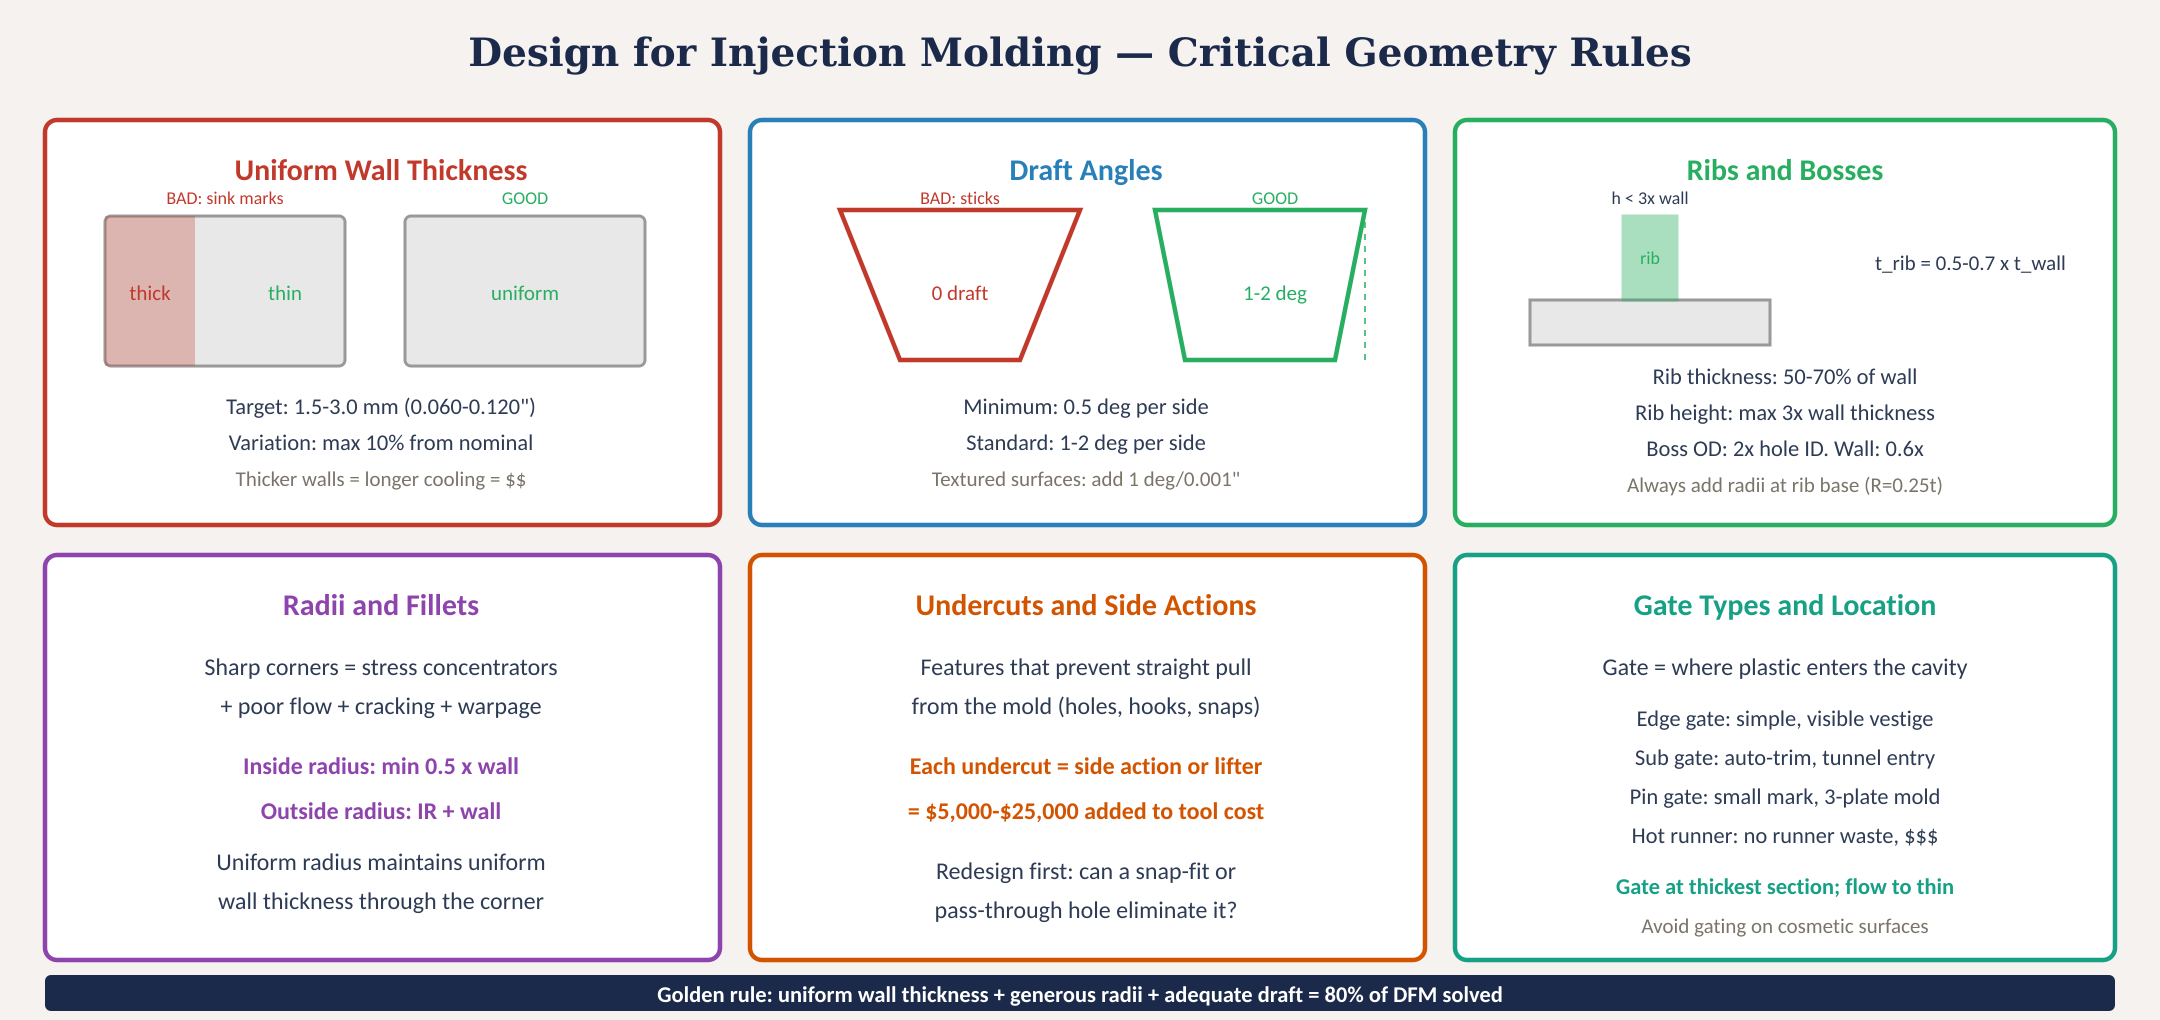
\includegraphics[width=\textwidth]{Designing for Injection Molding/fig_dfm_rules.png}
\caption{Six critical DFM geometry rules: wall thickness, draft angles, ribs/bosses, radii, undercuts, and gate location.}
\label{fig:dfm}
\end{figure}

\subsection{Rule 1: Uniform Wall Thickness}

The single most important design parameter. Wall thickness drives cycle time (cooling $\propto t^2$), material usage, shrinkage uniformity, and defect susceptibility.

\textbf{Recommended ranges}: ABS: 1.5--3.5\,mm. PC: 1.5--3.5\,mm. PP: 0.8--3.0\,mm. Nylon: 1.0--3.0\,mm. POM: 1.0--3.0\,mm.

\textbf{Uniformity}: Variation $<$10\% of nominal. Where transitions are unavoidable, use gradual tapers at a 3:1 length-to-thickness-change ratio. Abrupt steps cause differential shrinkage, sink marks, and stress concentrations.

\textbf{Coring out}: Replace solid thick sections with thin uniform shells reinforced by ribs. A ribbed 2\,mm wall is stiffer than a solid 4\,mm wall, cools in one-quarter the time, and uses half the material.

\subsection{Rule 2: Draft Angles}

Draft is the slight taper on walls parallel to the mold opening direction that allows the part to release.

\begin{itemize}[nosep,leftmargin=1.5em]
  \item Minimum: \ang{0.5} per side (tight tolerance applications).
  \item Standard: \ang{1}--\ang{2} per side (recommended).
  \item Textured surfaces: add \ang{1} per 0.001\,in (0.025\,mm) of texture depth.
  \item Core side often needs more draft than cavity side (part shrinks onto core).
\end{itemize}

\needspace{4\baselineskip}
\begin{warningbox}[Zero-Draft = Stuck Parts]
Zero-draft vertical walls are the \#1 student DFM error. Without draft, the part grips the core, ejector pins push through the wall, and the mold wears rapidly. Apply draft to \emph{all} surfaces parallel to the pull direction --- including internal ribs, bosses, and walls.
\end{warningbox}

\subsection{Rule 3: Ribs and Bosses}

Ribs add stiffness without mass; bosses provide screw/insert mounting points.

\subsubsection{Rib Proportions}
\begin{itemize}[nosep,leftmargin=1.5em]
  \item Thickness: 50--70\% of adjoining wall (thicker $\to$ sink marks on opposite surface).
  \item Height: max $3\times$ wall thickness (taller $\to$ fill and ejection problems).
  \item Draft: min \ang{0.5} per side (\ang{1} preferred).
  \item Spacing: min $2\times$ wall thickness between ribs.
  \item Base radius: 0.25--0.5 $\times$ wall thickness.
  \item Multiple thin ribs outperform one thick rib.
\end{itemize}

\subsubsection{Boss Proportions}
\begin{itemize}[nosep,leftmargin=1.5em]
  \item OD: 2.0--2.5 $\times$ screw/insert hole ID.
  \item Wall: 0.6 $\times$ nominal wall thickness.
  \item Freestanding bosses: connect to nearest wall with a rib.
  \item Height: max 2.5 $\times$ OD.
  \item For heat-set brass inserts: hole ID per insert manufacturer specification.
\end{itemize}

\subsection{Rule 4: Radii and Fillets}

Sharp inside corners create stress concentrations (up to $3\times$ at zero radius), impede melt flow, and cause sink marks.

\begin{itemize}[nosep,leftmargin=1.5em]
  \item Inside radius: min $0.5\times$ wall (1$\times$ preferred).
  \item Outside radius: inside radius $+$ wall thickness.
  \item This maintains uniform wall thickness through the corner.
  \item Apply radii to \emph{every} inside corner without exception.
\end{itemize}

\subsection{Rule 5: Undercuts}

Any feature preventing straight-pull mold separation --- side holes, snap hooks, internal threads, louvers. Each undercut requires a side action (cam, lifter, or collapsing core), adding \$5,000--\$25,000 to tooling cost.

\textbf{Always redesign first}: Can a pass-through hole replace a blind side hole? Can a snap-fit be oriented along the pull direction? Can an internal thread become a heat-set insert installed after molding?

\needspace{4\baselineskip}
\begin{tipbox}[Steel Safe Design]
Adding plastic to a molded part requires \emph{removing} steel from the mold. Removing steel (machining) is straightforward and inexpensive. Adding steel (welding and re-machining) is expensive and often compromises mold quality. The principle of ``steel safe'' design means intentionally making critical features slightly undersized in the mold (i.e., more steel than needed). After the first molding trial, you measure the parts, then remove steel to fine-tune dimensions. This iterative approach is standard practice and much cheaper than guessing wrong in the other direction. Design your critical dimensions steel safe and plan for at least one round of mold adjustment.
\end{tipbox}

\subsection{Rule 6: Gate Location}

The gate is where plastic enters the cavity.

\begin{itemize}[nosep,leftmargin=1.5em]
  \item \textbf{Place at the thickest section} so melt flows from thick to thin (ensures adequate packing).
  \item \textbf{Never gate on a cosmetic surface} --- the gate vestige is always visible.
  \item Gate types: edge gate (simple, visible mark), sub gate (auto-trimmed), pin gate (small mark, 3-plate mold), hot runner (no runner waste, highest tooling cost).
  \item Flow simulation (Moldflow) predicts fill pattern and weld line locations.
\end{itemize}


% ══════════════════════════════════════════════════════════════════════
\FloatBarrier
\section{Common Defects}
\label{sec:defects}
% ══════════════════════════════════════════════════════════════════════

Every defect has a root cause in part geometry, material, or process. Good design eliminates most defects before the mold is ever cut.

\begin{figure}[ht!]
\centering
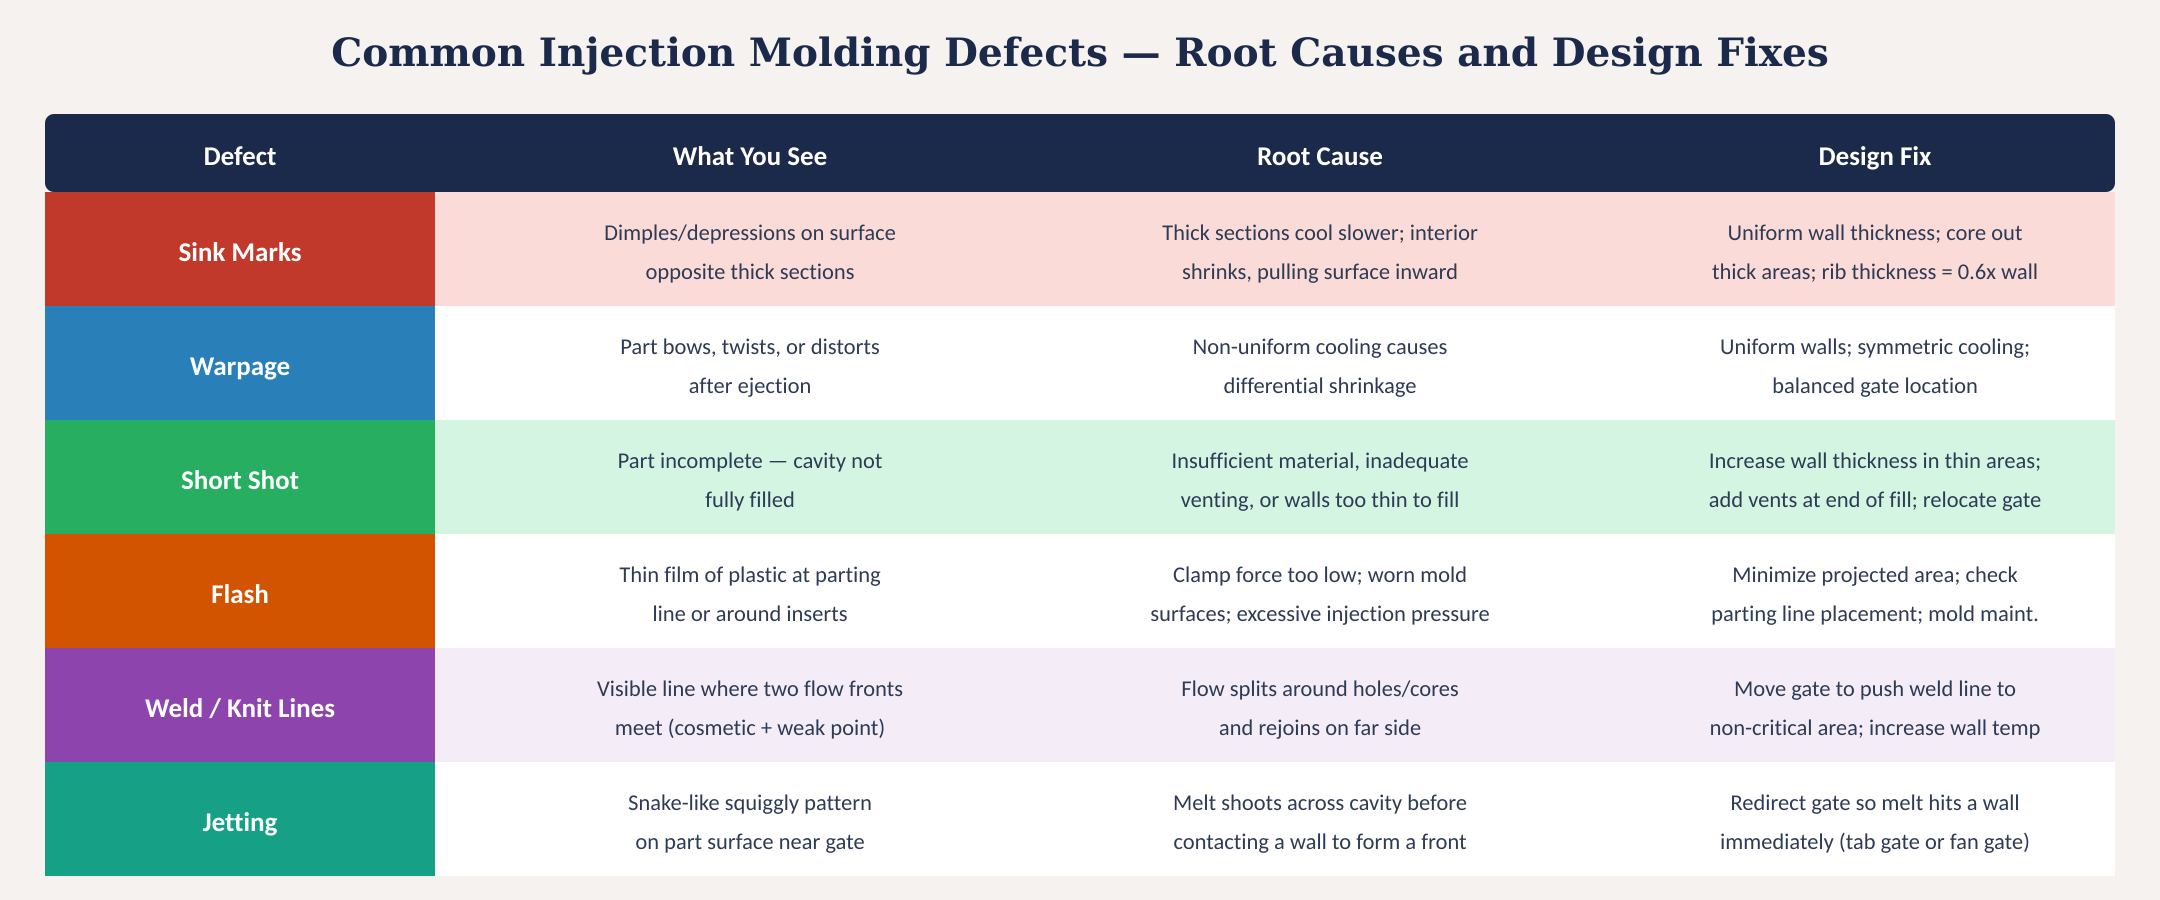
\includegraphics[width=\textwidth]{Designing for Injection Molding/fig_defects.png}
\caption{Six common injection molding defects with visual description, root cause, and design fix.}
\label{fig:defects}
\end{figure}

\begin{table}[ht!]
\centering\small
\begin{tabularx}{\textwidth}{l l X X}
  \toprule
  \textbf{Defect} & \textbf{What You See} & \textbf{Root Cause} & \textbf{Design Fix} \\
  \midrule
  Sink marks & Dimples opposite thick sections & Thick areas cool slowly, interior shrinks & Uniform walls; core out; rib = 0.6$\times$ wall \\
  Warpage & Part bows/twists after ejection & Non-uniform cooling $\to$ differential shrinkage & Uniform walls; symmetric cooling; balanced gate \\
  Short shot & Incomplete part & Inadequate venting, thin walls, low pressure & Vent at end of fill; increase thin walls \\
  Flash & Thin film at parting line & Low clamp force, worn mold, high pressure & Minimize projected area; mold maintenance \\
  Weld lines & Visible line where fronts meet & Flow splits around holes/cores & Relocate gate; increase melt temperature \\
  Jetting & Squiggly pattern near gate & Melt shoots across cavity before wall contact & Redirect gate so melt hits a wall immediately \\
  \bottomrule
\end{tabularx}
\caption{Common defects, root causes, and design fixes.}
\end{table}

\needspace{4\baselineskip}
\begin{tipbox}[Weld Line Strength]
Weld lines retain only 50--90\% of base material strength. If a weld line falls on a load-bearing feature, relocate the gate or add ribs to reinforce. Flow simulation is the primary tool for predicting and relocating weld lines before cutting the mold.
\end{tipbox}


% ══════════════════════════════════════════════════════════════════════
\FloatBarrier
\section{Warpage}
\label{sec:warp}
% ══════════════════════════════════════════════════════════════════════

Warpage is dimensional distortion that occurs after the part is ejected from the mold. It is caused by differential shrinkage---different regions of the part shrinking by different amounts. Warpage is one of the most difficult defects to predict and correct because it results from the interaction of multiple factors.

\subsection{Causes of Warpage}

\textbf{Material type}: Amorphous polymers (ABS, PC) have randomly oriented molecular chains that shrink relatively uniformly in all directions, typically 0.4--0.8\%. Semi-crystalline polymers (PP, nylon, POM) form crystalline structures during cooling that pack more tightly, resulting in higher overall shrinkage (1.0--2.5\%) and greater directional variation. Semi-crystalline materials are inherently more prone to warpage than amorphous ones.

\textbf{Fiber and molecular orientation}: As molten plastic flows through the cavity, polymer molecules and any reinforcing fibers (glass, carbon) align in the direction of flow. This creates anisotropic shrinkage---the part shrinks differently parallel versus perpendicular to flow. For glass-filled materials, this effect is pronounced: the part may shrink 0.3\% along the flow direction but 0.8\% across it. The gate location determines the flow pattern and therefore the orientation pattern. Changing gate position changes the warp behavior.

\textbf{Varying wall thickness}: Thick sections cool more slowly than thin sections, creating differential shrinkage across the part. The thick section is still contracting when the thin section has already solidified, setting up internal stresses that cause bowing or twisting after ejection.

\textbf{Mold-induced constraint}: While the part is in the mold, the steel surfaces physically restrain shrinkage. The part shrinks \emph{onto} core features (gripping them tighter) and \emph{away from} cavity surfaces (releasing from them). This constrained shrinkage creates internal stresses that are ``frozen in.'' After ejection, as the part continues to cool and these stresses relax, the part warps.

\textbf{Gate location and packing}: The part is filled from the gate outward. Material near the gate receives higher packing pressure and is denser than material at the end of fill. This density gradient creates a shrinkage gradient from gate to end of fill, contributing to warpage.

\subsection{Designing to Minimize Warpage}
\begin{enumerate}[leftmargin=1.5em]
\item Maintain \textbf{uniform wall thickness} throughout the part---the single most effective warp-reduction strategy.
\item Choose \textbf{amorphous materials} when dimensional stability is critical and material properties allow.
\item Consider \textbf{gate location} to control flow direction. For parts where strength directionality matters, orient flow to align fibers with the primary load path.
\item Use \textbf{flow simulation} (Moldflow, Moldex3D) to predict warp before cutting the mold.
\item Add \textbf{stiffening features} (ribs, gussets) to resist warp in vulnerable areas.
\end{enumerate}

% ══════════════════════════════════════════════════════════════════════
\FloatBarrier
\section{Surface Finish}
\label{sec:surface}
% ══════════════════════════════════════════════════════════════════════

The surface of the molded part is a direct replica of the mold surface. A polished mold produces a glossy part; a textured mold produces a textured part. Surface finish affects both aesthetics and function.

\subsection{SPI (PIA) Finish Standards}
The Plastics Industry Association defines four categories of mold surface finish:

\begin{center}
\small
\begin{tabularx}{\textwidth}{l l X}
\toprule
\textbf{Grade} & \textbf{Method} & \textbf{Application} \\
\midrule
A-1 to A-3 & Diamond buff (Grade \#3 to \#15) & Optical clarity, mirror finish, lenses \\
B-1 to B-3 & Paper polish (600 to 320 grit) & Semi-gloss, good appearance \\
C-1 to C-3 & Stone polish (600 to 320 grit) & Matte, removes machining marks \\
D-1 to D-3 & Dry blast (glass bead or oxide) & Textured, hides sink marks and flow lines \\
\bottomrule
\end{tabularx}
\end{center}

Higher-quality finishes (A-grades) require more labor and cost more. Each finish level builds on the previous one---you polish to B-grade before diamond-buffing to A-grade. For student projects, C-2 or C-3 is typically adequate for cosmetic surfaces, and as-machined (no additional finishing) is acceptable for non-cosmetic surfaces.

\subsection{Textured Surfaces and Draft}
Textured surfaces (acid-etched, laser-engraved, or EDM-finished) act as microscopic undercuts during ejection. The more aggressive the texture, the more draft angle is required to allow the part to release cleanly. The standard rule is: add \ang{1} of draft per 0.001\,in (0.025\,mm) of texture depth, in addition to the baseline draft. A surface with 0.003\,in texture depth needs an additional \ang{3} of draft. Insufficient draft on textured surfaces causes drag marks that damage both the part surface and the mold steel.

\needspace{4\baselineskip}
\begin{tipbox}[Surface Finish Strategy]
It is common to specify different finishes on different surfaces of the same part. The A-side (show surface) may have a specific texture for appearance, while the B-side has a rougher finish to promote part retention on the ejection side during mold opening and to reduce finishing cost. Specifying the finish at CDR is important because texturing is typically the last step in mold construction.
\end{tipbox}

% ══════════════════════════════════════════════════════════════════════
\FloatBarrier
\section{Insert Molding and Overmolding}
\label{sec:overmold}
% ══════════════════════════════════════════════════════════════════════

\subsection{Insert Molding}
Insert molding involves placing a pre-formed component (typically metal) into the mold cavity before injection. The plastic flows around and encapsulates the insert, creating a single integrated part. Common applications include threaded brass inserts for screw-assembly, electrical terminals, and structural reinforcements.

\textbf{Design considerations for inserts}: The insert must resist pull-out forces and rotational torque. Knurled surfaces and undercuts on the insert provide mechanical interlocking with the plastic. The insert must be properly positioned in the mold---for low-volume production, a human operator loads each insert manually; for high-volume production, robotic loading or bowl feeders automate the process. Ensure adequate plastic wall thickness around the insert (minimum $2\times$ the insert diameter) to prevent cracking from the stress concentration.

An alternative to insert molding is \textbf{heat-set inserts}: brass inserts with helical knurling that are pressed into a pre-molded hole using a heated tip after molding. Heat-set inserts are simpler (no mold modification needed) and are the standard approach for adding threaded fastening points to 3D-printed and low-volume molded parts.

\subsection{Overmolding}
Overmolding is molding one material over another---typically a soft thermoplastic elastomer (TPE) over a rigid substrate (ABS, PC, nylon). Applications include soft-touch grips on power tools, rubber seals on enclosures, and non-slip surfaces on handheld devices.

\textbf{Material compatibility} is critical: the overmold material must chemically bond to the substrate. TPE manufacturers publish compatibility charts showing which substrates their materials adhere to. Common compatible pairs include TPE over ABS, TPE over PC, and TPE over nylon. PP substrates require special TPE grades.

\textbf{Design considerations}: The overmold material needs a flow path from the gate to all overmolded areas. For parts with overmold on both sides of the substrate, design \textbf{through-holes} in the substrate so plastic can flow from one side to the other. Avoid thin overmold sections ($< 1$\,mm) as they are difficult to fill and may delaminate.

% ══════════════════════════════════════════════════════════════════════
\FloatBarrier
\section{Living Hinges and Snap-Fit Clips}
\label{sec:hinges}
% ══════════════════════════════════════════════════════════════════════

\subsection{Living Hinges}
A living hinge is a thin, flexible web of plastic that connects two rigid sections of a single molded part, allowing them to fold relative to each other. The most common application is the flip-top cap on a shampoo bottle. Living hinges eliminate the need for separate hinge hardware and reduce assembly steps.

\textbf{Material selection} is the most critical factor. Only semi-crystalline materials with high fatigue resistance should be used: \textbf{polypropylene (PP)} is the gold standard (can survive millions of flex cycles), followed by \textbf{polyethylene (PE)}. Amorphous materials (ABS, PC) will crack after very few cycles and are unsuitable for living hinges.

\textbf{Design rules}: The hinge section is typically 0.2--0.4\,mm thick (0.008--0.015\,in)---thin enough to flex without cracking but thick enough to maintain structural integrity. The hinge web should be slightly thicker initially (``steel safe'') and thinned after the first molding trial. Gate location must direct material flow \textbf{perpendicular to the hinge} so that polymer chains orient across the hinge axis, maximizing flex strength. Never place a weld line at the hinge---weld lines have reduced strength and will cause premature failure.

\needspace{4\baselineskip}
\begin{warningbox}[Flex Immediately After Molding]
Living hinges in PP should be flexed to their full range immediately after ejection from the mold, while the plastic is still warm. This initial flex orients the polymer chains in the hinge zone and dramatically improves fatigue life. Failing to do this initial flex can result in a hinge that cracks on first use.
\end{warningbox}

\subsection{Snap-Fit Clips}
Snap-fit clips are cantilever beams molded into the part that deflect during assembly and lock into a mating feature. They are the most common method for assembling injection-molded enclosures because they eliminate fasteners, reduce assembly time, and can be designed for both permanent and releasable connections.

\textbf{Design parameters}: The clip arm must be long enough to flex without exceeding the material's yield strain. For a cantilever snap:

\begin{equation}
\varepsilon_{\max} = \frac{3 \cdot y \cdot t}{2 \cdot L^2}
\end{equation}

where $y$ is the deflection (undercut depth), $t$ is the beam thickness, and $L$ is the beam length. The maximum allowable strain depends on the material: PP can tolerate up to 5\%, ABS up to 2\%, and PC up to 1.5\% for repeated use. For one-time assembly (permanent clips), higher strains are acceptable.

\textbf{Mold considerations}: If the clip undercut is in the line of draw, it can be molded directly. If the undercut is perpendicular to the line of draw, it creates a true undercut requiring a side action. You can often avoid the side action by designing a \textbf{pass-through hole} behind the clip---one mold half protrudes through the hole to form the undercut feature, then retracts during ejection.


% ══════════════════════════════════════════════════════════════════════
\FloatBarrier
\section{Tooling and Economics}
\label{sec:tooling}
% ══════════════════════════════════════════════════════════════════════

\begin{figure}[ht!]
\centering
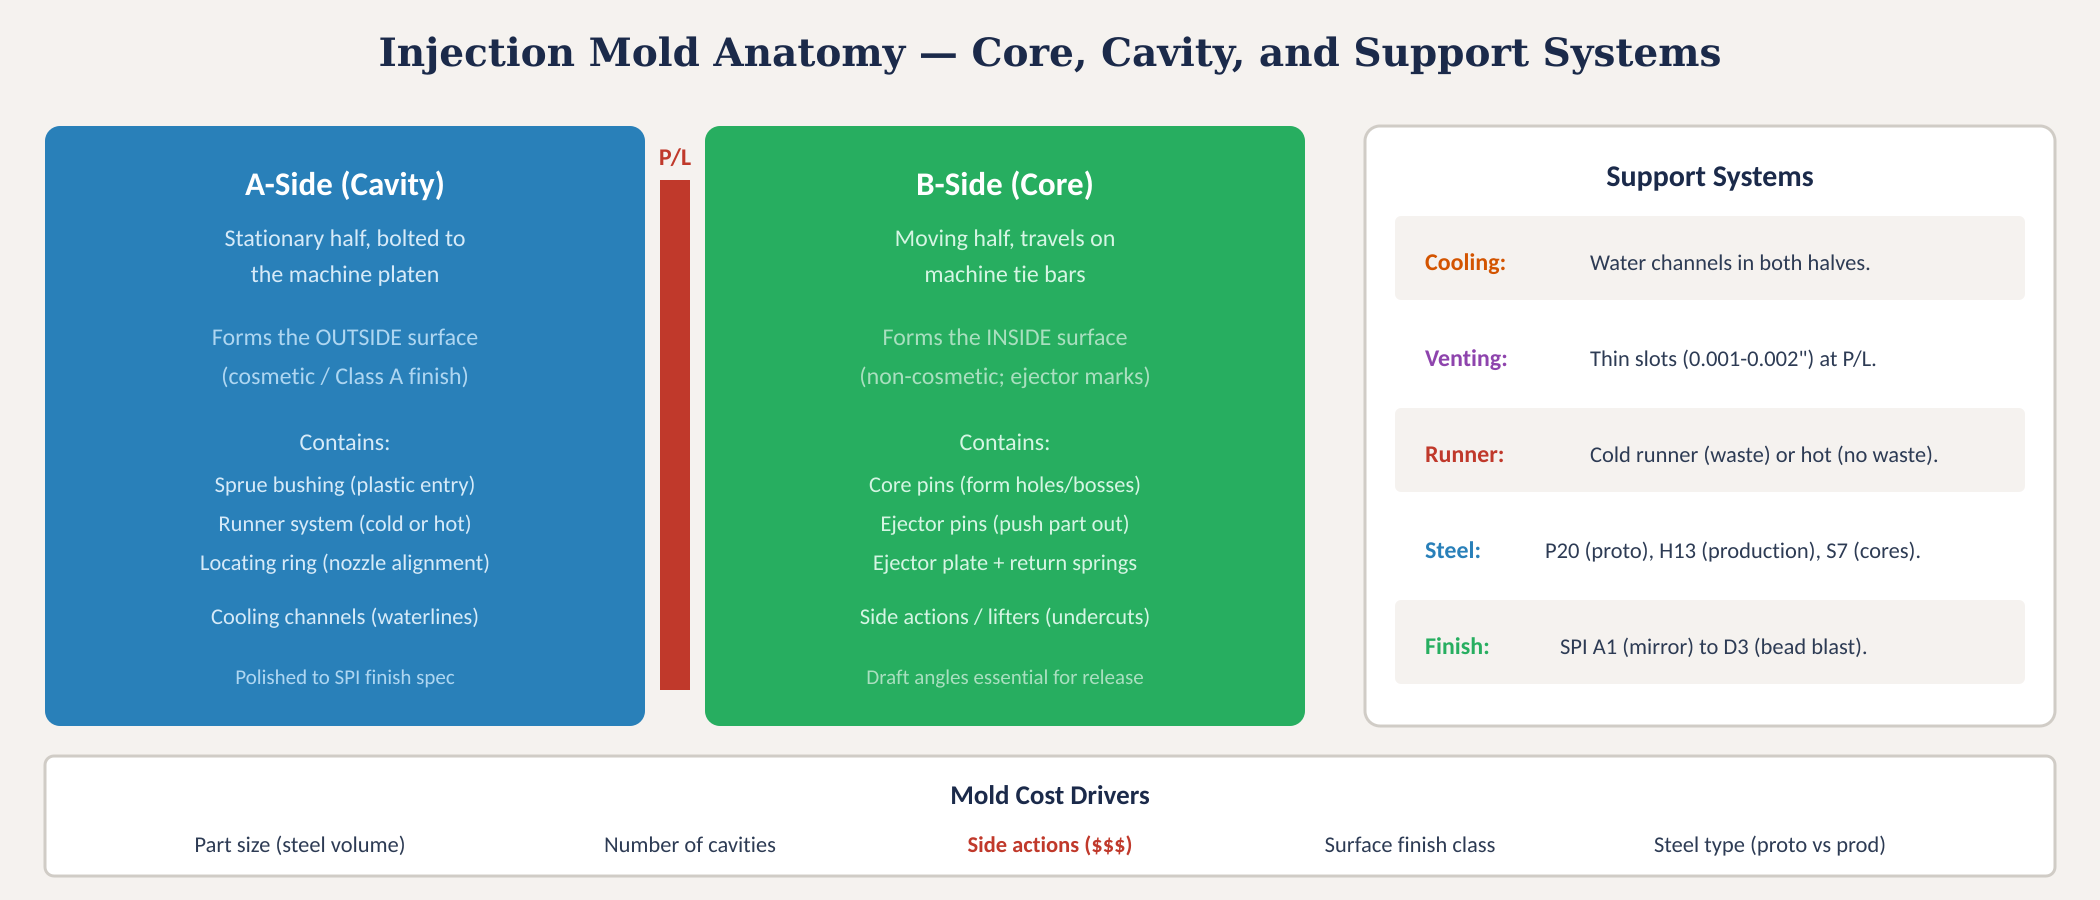
\includegraphics[width=\textwidth]{Designing for Injection Molding/fig_mold_anatomy.png}
\caption{Mold anatomy: A-side (cavity), B-side (core), parting line, support systems, and cost drivers.}
\label{fig:mold}
\end{figure}

\subsection{Mold Construction}

The \textbf{A-side} (cavity) forms the cosmetic outside surface. It contains the sprue bushing, runner system, and locating ring. Surfaces are polished to SPI specifications (A-1 mirror to D-3 bead blast). The \textbf{B-side} (core) forms the inside surface and contains core pins, ejector pins, ejector plates, and side actions. The parting line between the halves leaves a witness mark on the part.

\textbf{Support systems}: cooling channels (water lines in both halves; conformal cooling can reduce cycle time 20--40\%), venting (thin slots 0.001--0.002\,in at parting line), runner system (cold runner produces waste; hot runner eliminates waste but costs more), and ejection system (pins, sleeves, blades, stripper plates).

\subsection{Mold Classifications (SPI)}

\begin{table}[ht!]
\centering\small
\begin{tabularx}{\textwidth}{l l l l X}
  \toprule
  \textbf{Class} & \textbf{Steel} & \textbf{Life (cycles)} & \textbf{Cost Range} & \textbf{Use} \\
  \midrule
  105 (Prototype) & Aluminum / soft steel & $<$500 & \$5K--\$15K & Design validation, pilot runs \\
  104 (Low Prod.) & P20 pre-hardened & $<$100K & \$15K--\$50K & Low volume, bridge tooling \\
  103 (Med. Prod.) & H13 hardened & $<$500K & \$30K--\$80K & Medium-volume production \\
  101 (High Prod.) & Premium hardened & 1M+ & \$50K--\$200K+ & High-volume, long-life production \\
  \bottomrule
\end{tabularx}
\caption{SPI mold classifications.}
\end{table}

\subsection{Part Cost Economics}

\begin{equation}
  C_{\text{part}} = C_{\text{material}} + C_{\text{cycle}} + C_{\text{tooling,amortized}}
\end{equation}

where $C_{\text{material}} = \text{weight (g)} \times \text{resin cost (\$/g)}$, $C_{\text{cycle}} = \text{cycle time (s)} \times \text{machine rate (\$/hr)} / 3600$, and $C_{\text{tooling}} = \text{mold cost} / \text{expected lifetime parts}$.

\textbf{Example} (small ABS enclosure, 30\,g): Material: $30 \times \$0.002 = \$0.06$. Cycle (25\,s at \$60/hr): $\$0.42$. Tooling (\$25K / 50K parts): $\$0.50$. \textbf{Total: \$0.98/part}. At 500K parts, tooling drops to \$0.05/part $\to$ total \$0.53/part.

Injection molding breaks even versus 3D printing at approximately 100--500 parts depending on part size and complexity. Below that, 3D printing is cheaper; above it, injection molding wins dramatically.


% ══════════════════════════════════════════════════════════════════════
\FloatBarrier
\section{DFM Checklist}
\label{sec:checklist}
% ══════════════════════════════════════════════════════════════════════

Review every item before sending your CAD model to a molder.

\begin{enumerate}[leftmargin=1.5em]
  \item Wall thickness uniform ($\pm$10\%)? Within recommended range for material?
  \item Draft angles applied to ALL surfaces parallel to pull direction? Texture draft added?
  \item Ribs at 50--70\% of wall? Height $\leq 3\times$ wall? Base radii present?
  \item Bosses at $2\times$ hole ID? Connected to walls with ribs? Boss wall $\leq 0.6\times$ nominal?
  \item All inside corners radiused (min $0.5\times$ wall)? Outside radius = inside + wall?
  \item Undercuts identified? Side actions justified or redesigned out?
  \item Gate location at thickest section? Not on cosmetic surface?
  \item Parting line location acceptable on finished part?
  \item Ejector pin locations on non-cosmetic surfaces? Adequate draft for release?
  \item Shrinkage accounted for in critical dimensions? Tolerances achievable ($\pm$0.005\,in typical)?
  \item Material selected? Properties verified against operating conditions?
  \item Moldflow or fill analysis run? Weld lines and air traps identified?
\end{enumerate}

\needspace{4\baselineskip}
\begin{warningbox}[Fix Problems in CAD, Not in Steel]
Fixing a design problem in CAD takes minutes. Finding the same problem after the mold is cut costs \$5,000--\$20,000 in mold modifications and 2--4 weeks of delay. Run this checklist at your CDR before committing to tooling.
\end{warningbox}


% ══════════════════════════════════════════════════════════════════════
\FloatBarrier
\section{Practice Questions}
\label{sec:practice}
% ══════════════════════════════════════════════════════════════════════

\subsection{Conceptual Questions}

\begin{enumerate}[leftmargin=1.5em]
  \item Why does cooling time scale with the \emph{square} of wall thickness rather than linearly? How does this affect part cost?

  \item A part has a 4\,mm thick boss connected to a 2\,mm wall. Predict the defect you will see on the surface opposite the boss. What is the design fix?

  \item Explain why a part shrinks onto the core side of the mold during cooling. How does this affect draft angle requirements for the core versus cavity sides?

  \item Your part has a snap hook that creates an undercut on one side. The molder quotes \$18,000 for the side action. Propose two redesign alternatives that might eliminate the side action.

  \item Compare ABS and polypropylene for a consumer electronics enclosure that must accept paint and withstand a 1-meter drop test. Which do you recommend and why?

  \item Why must the gate be placed at the thickest section? What happens if you gate at a thin section instead?

  \item A textured surface (SPI D-2, depth $\approx$ 0.002\,in) on a 3-inch-deep wall currently has \ang{1} of draft. Is this sufficient? If not, what is the correct draft angle?
\end{enumerate}

\subsection{Application / Scenario Questions}

\begin{enumerate}[resume,leftmargin=1.5em]
  \item You are designing a two-piece snap-fit enclosure for an IoT sensor that will be installed outdoors. The enclosure must be IP65, withstand $-20$ to $+60$\,\degC, resist UV for 5+ years, and cost under \$3/part at 10,000 units. Select the material, specify wall thickness, describe the snap-fit design, and estimate whether injection molding is economically justified.

  \item Your teammate's CAD model for a motor mount bracket has: 5\,mm walls, zero draft on all vertical surfaces, sharp inside corners, and a boss with OD = 1.5$\times$ hole ID. List every DFM violation, predict the defects that will result from each, and specify the corrected dimensions.

  \item \textbf{Cost analysis}: A part weighs 45\,g in PC/ABS (\$0.003/g). Cycle time is 30\,seconds on a machine at \$75/hr. The mold costs \$35,000. Calculate the total part cost at 5,000, 50,000, and 500,000 units. At what volume does injection molding become cheaper than SLA 3D printing at \$8.50/part?
\end{enumerate}

\subsection{Answers}

\begin{enumerate}[leftmargin=1.5em]
  \item Cooling is a transient heat-conduction problem governed by the Fourier equation. The characteristic time for heat to diffuse through a slab of thickness $t$ scales as $t^2 / \alpha$ where $\alpha$ is thermal diffusivity. Doubling wall thickness from 2\,mm to 4\,mm quadruples cooling time --- potentially adding 20--40 seconds per cycle. At a machine rate of \$60/hr, each additional second costs approximately \$0.017/part. Over 100,000 parts, a 20-second cycle-time penalty costs \$17,000.

  \item A sink mark (dimple/depression) on the surface opposite the boss. The 4\,mm boss is twice the 2\,mm wall, creating a thick section that cools more slowly. The interior shrinks and pulls the surface inward. Fix: reduce boss wall to $0.6 \times 2 = 1.2$\,mm (OD = hole ID + 2$\times$1.2\,mm). Connect the boss to the nearest wall with a thin rib.

  \item As plastic cools it contracts volumetrically. The cavity half forms the outside surface, and the part shrinks \emph{away} from it, naturally releasing. The core half forms the inside surface, and the part shrinks \emph{onto} it, gripping tighter as it cools. This means the core side typically needs more draft (\ang{1.5}--\ang{2}) than the cavity side (\ang{0.5}--\ang{1}) to overcome the shrink-grip.

  \item (a) Reorient the snap hook to flex along the mold-open direction --- if the hook can deflect during ejection, no side action is needed (the hook ``snaps'' past the mold surface). (b) Replace the snap hook with a separate clip that installs post-molding via a push-fit or ultrasonic weld, eliminating the undercut entirely.

  \item ABS. Both have adequate impact strength, but ABS accepts paint directly (smooth surface, good adhesion) while PP requires flame treatment or specialty primers due to its low surface energy. ABS also has a higher HDT ($\sim$95\,$^{\circ}$C versus $\sim$60\,$^{\circ}$C for unfilled PP), providing more thermal margin. ABS shrinkage (0.5--0.7\%) is lower and more predictable than PP (1.0--2.5\%), enabling tighter dimensional control for snap-fits and mating features.

  \item Gating at the thickest section ensures that the section that shrinks the most remains connected to the runner for packing pressure the longest. If you gate at a thin section, the thin area freezes first and seals off (``gates off''), cutting the thick section off from packing pressure. The result is severe sink marks and voids in the thick section because the material cannot be replenished as it shrinks.

  \item No. The texture-depth rule requires adding \ang{1} per 0.001\,in of depth. At 0.002\,in depth, add \ang{2} beyond the standard \ang{1} for a total of \ang{3} per side. Without adequate draft, the textured surface acts like sandpaper during ejection, leaving drag marks that ruin the finish and gouge the mold steel.

  \item Material: ASA (acrylic-styrene-acrylonitrile) --- UV-stable variant of ABS, good impact from $-20$ to $+80$\,\degC, IP65-rated with proper gasket design, paintable if needed. Wall thickness: 2.0\,mm nominal (meets structural requirements, enables IP65 with perimeter gasket groove). Snap-fit: cantilever snaps along the mold-open axis (no side action), 2\% max strain for ASA, designed with \ang{1.5} draft. Economics: at 10,000 units with a Class~104 mold (\$25K), tooling amortization is \$2.50/part. Material (20\,g $\times$ \$0.003): \$0.06. Cycle (20\,s at \$60/hr): \$0.33. Total: $\sim$\$2.89/part --- under the \$3 target. Injection molding is justified.

  \item Violations and fixes: (a) 5\,mm walls are too thick for any common plastic --- excessive cooling time, sink marks, voids. Fix: core out to 2\,mm uniform walls, add ribs for stiffness. (b) Zero draft on all vertical surfaces --- parts will stick, ejector damage, mold wear. Fix: add minimum \ang{1} per side to all surfaces parallel to pull. (c) Sharp inside corners --- stress concentrations ($3\times$ multiplier), impeded flow. Fix: add $R = 0.5 \times 2 = 1$\,mm fillet to all inside corners; outside radius = $1 + 2 = 3$\,mm. (d) Boss OD at $1.5\times$ hole ID is too thin-walled, creating a thick ring that sinks. Fix: increase OD to $2.0\times$ hole ID. Predicted defects: sink marks everywhere (thick walls + oversized boss), warpage (non-uniform cooling from variable thickness), ejection damage (no draft), cracking at corners under load (no radii).

  \item Material: $45 \times 0.003 = \$0.135$/part. Cycle: $30/3600 \times 75 = \$0.625$/part. These are constant.

  At 5,000 parts: tooling $= 35000/5000 = \$7.00$/part. Total: $\$7.76$/part.

  At 50,000 parts: tooling $= 35000/50000 = \$0.70$/part. Total: $\$1.46$/part.

  At 500,000 parts: tooling $= 35000/500000 = \$0.07$/part. Total: $\$0.83$/part.

  Break-even vs.\ SLA at \$8.50/part: solve $0.135 + 0.625 + 35000/n = 8.50$. $35000/n = 7.74$. $n = 4,522$ parts. Above $\sim$4,500 parts, injection molding is cheaper.
\end{enumerate}


% ══════════════════════════════════════════════════════════════════════




\part{Major Project Milestones}

This section provides a comprehensive guide to the three formal design reviews that structure the MEGN~301 project lifecycle. Each review is a gate: the team must demonstrate a specific level of design maturity before advancing to the next phase. The three reviews answer progressively deeper questions about the design:

\begin{center}
\small
\begin{tabularx}{\textwidth}{l l X}
\toprule
\textbf{Review} & \textbf{Core Question} & \textbf{What the Team Demonstrates} \\
\midrule
\textbf{PDR} & ``Should this work?'' & The design concept is feasible, viable, desirable, and sustainable. The problem is well-defined, requirements are established, and a defensible concept has been selected. \\
\textbf{CDR} & ``Will this work?'' & The design is complete enough to build. Every component is specified, every interface is defined, every risk is mitigated, and the manufacturing plan is ready. \\
\textbf{FDR} & ``How well did it work?'' & The built system has been tested against every requirement. Results, deviations, lessons learned, and future recommendations are documented. \\
\bottomrule
\end{tabularx}
\end{center}

Each chapter in this section maps the review's deliverables to the technical content in Parts~I and~II, tells you exactly what artifacts to produce, and provides evaluation criteria so you know what ``good'' looks like before you present.

\begin{figure}[ht!]\centering
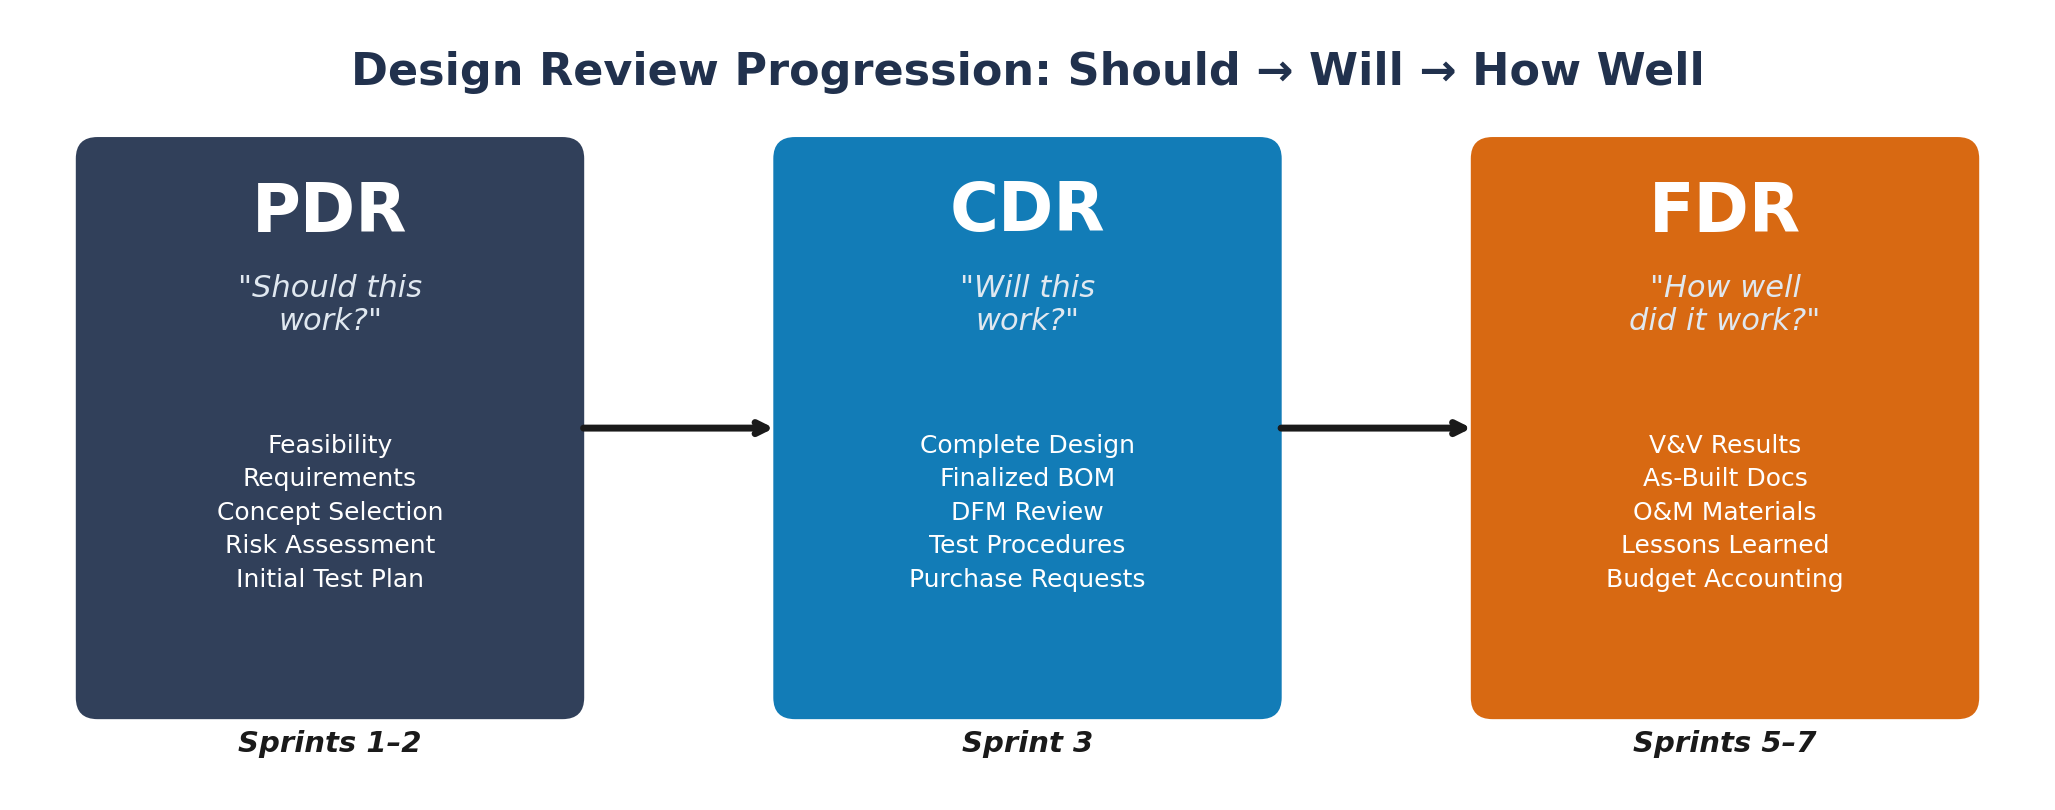
\includegraphics[width=\textwidth]{Project Milestones/fig_review_progression.png}
\caption{Design review progression: PDR validates feasibility, CDR validates completeness, FDR validates performance. Each review gates advancement to the next project phase.}\label{fig:reviews}
\end{figure}

\FloatBarrier
\section*{The Complete Artifact Progression}
\addcontentsline{toc}{section}{The Complete Artifact Progression}

The following table is the \textbf{meta-artifact} for your entire project. It shows how every document evolves from PDR through CDR to FDR. Print this page and bring it to every design review to confirm you have not missed anything. There is no ``starting over'' between reviews---you are maturing the \emph{same} set of documents across the semester.

\begin{center}
\small
\begin{tabularx}{\textwidth}{l l X X X}
\toprule
\textbf{Artifact} & \textbf{Ch.} & \textbf{PDR State} & \textbf{CDR State} & \textbf{FDR State} \\
\midrule
Problem Statement & 1 & Finalized & Unchanged & Unchanged \\
ConOps & 1 & Finalized & Updated if needed & Validated against \\
SDRD / Requirements & 2 & Initial version & Updated with changes & Final version with change history \\
RTM & 2 & Reqs $\to$ needs traced & Reqs $\to$ subsystems allocated & Every req verified with status \\
Architecture & 2 & Preliminary block diagram & Detailed with ICDs & As-built (deviations noted) \\
Trade Study & 3 & Complete with selection & Unchanged & Referenced in design evolution \\
FMEA & 3/6 & Initial (concept-level) & Updated (detail design) & Final (with O\&M items) \\
BOM & 3 & Preliminary estimate & Detailed with costs \& Plan~B & As-built with actual costs \\
Test Plan & 4 & Methods assigned & Procedures written & Executed with results \\
VCRM & 4 & All ``Open'' & Methods \& procedures assigned & All statuses final \\
CAD / Drawings & 3 & Concept sketches & Fully dimensioned & As-built (deviations noted) \\
Wiring Diagrams & 3 & Preliminary & Complete & As-built \\
Software & --- & Pseudocode / flowchart & Source code v1.0 & Final version \\
O\&M Materials & 6 & Not yet & Identified needs & Complete package \\
\bottomrule
\end{tabularx}
\end{center}


% ═══════════════════════════════════════════════════════════════
\FloatBarrier
\chapter{Preliminary Design Review (PDR)}

\vspace{1em}

\begin{keyconceptbox}[Bottom Line]
PDR answers the question: \textbf{``Should this design work?''} The team demonstrates that the problem is well-understood, the requirements are sound, competing concepts have been evaluated objectively, and the selected concept is feasible across technical, economic, schedule, and operational dimensions. PDR is not a commitment to a final design---it is a commitment to a \emph{direction} that the evidence supports. A PDR that cannot defend its concept selection with data has not earned the right to proceed.
\end{keyconceptbox}

\vspace{1em}

\FloatBarrier
\section{Purpose and Scope}

The Preliminary Design Review is the first formal gate in the project lifecycle. It corresponds to Sprints~1--2 in the MEGN~301 course structure and draws on content from Chapters~1--3 of Part~I. The purpose of PDR is to establish confidence that:

\begin{enumerate}[leftmargin=1.5em]
\item The \textbf{problem} is clearly defined, scoped, and worth solving (Chapter~1).
\item The \textbf{stakeholders} have been identified and their needs have been captured and prioritized (Chapter~1).
\item The \textbf{requirements} are formal, testable, traceable, and complete (Chapter~2).
\item Multiple \textbf{concepts} have been generated and evaluated against the requirements using objective methods (Chapter~3).
\item The selected concept is \textbf{feasible}---it can be built, afforded, completed on schedule, and will satisfy the stakeholder (Chapter~3).
\item The major \textbf{risks} have been identified, quantified, and have credible mitigation plans (Chapter~3).
\item A \textbf{test plan} exists that maps every requirement to a verification method (Chapter~4).
\end{enumerate}

PDR does \emph{not} require a finished design. It requires evidence that the team has done the front-end engineering work necessary to justify proceeding into detailed design.

\FloatBarrier
\section{PDR Deliverables}

\subsection{Problem Definition and Background Research}

\begin{itemize}[leftmargin=1.5em]
\item \textbf{Five-element problem statement} (Chapter~1): WHO, WHAT, WHERE, WHY IT MATTERS, CONSTRAINTS. Solution-agnostic. Reviewed and approved by the instructor (acting as sponsor/stakeholder).
\item \textbf{Market analysis} (Chapter~1): Competitive product survey with pros/cons table for at least three existing solutions. Patent search identifying two relevant utility patents with freedom-to-operate assessment.
\item \textbf{Customer discovery results} (Chapter~1): Summary of AI persona interviews. Validated customer needs organized by MoSCoW priority. Key insights that shaped the requirements.
\item \textbf{Stakeholder registry} (Chapter~1): All identified stakeholders classified on the power/interest grid with engagement strategies.
\item \textbf{Concept of Operations (ConOps)} (Chapter~1): Plain-language description of how the system will be used, including normal, degraded, and maintenance operational scenarios.
\end{itemize}

\subsection{System Requirements and Traceability}

\begin{itemize}[leftmargin=1.5em]
\item \textbf{System Design Requirements Document (SDRD)} (Chapter~2): Goal statement, objectives, and quantitative SHALL requirements organized in the three-level hierarchy. Every requirement must be clear, precise, quantifiable, and measurable.
\item \textbf{Requirements Traceability Matrix (RTM)} (Chapter~2): Initial version linking every requirement to its parent stakeholder need, requirement type (F/P/NFR), and assigned verification method (T/A/I/D). Status column: ``Open'' for all requirements at PDR.
\item \textbf{Functional decomposition} (Chapter~2): Verb-noun function hierarchy showing WHAT the system must do, without specifying HOW.
\item \textbf{Environmental and regulatory constraints} (Chapter~2): Operating conditions, applicable standards, and compliance requirements identified as non-functional requirements.
\end{itemize}

\subsection{Concept Development and Selection}

\begin{itemize}[leftmargin=1.5em]
\item \textbf{Reverse engineering analysis} (Chapter~3): Documented disassembly and analysis of the COTS product, including component inventory, interface inventory, and constraints on the add-on system.
\item \textbf{Concept generation evidence} (Chapter~3): Morphological chart built from the functional decomposition, with at least 3--5 implementation options per function. Evidence that divergent techniques (brainstorming, SCAMPER) were used.
\item \textbf{Concept screening} (Chapter~3): Pugh matrix showing qualitative evaluation of candidate concepts against a datum.
\item \textbf{Trade study} (Chapter~3): Weighted decision matrix with criteria derived from requirements, documented weight rationale, data-backed ratings, sensitivity analysis, and a clear recommendation. The trade study is the traceable evidence that the concept selection is rational, not arbitrary.
\item \textbf{Preliminary architecture} (Chapter~2): Block diagram of the selected concept showing subsystems, interfaces, and allocated functions.
\end{itemize}

\subsection{Risk and Feasibility}

\begin{itemize}[leftmargin=1.5em]
\item \textbf{FMEA} (Chapter~3/6): Failure modes identified for the selected concept. Severity, Occurrence, and Detection rated. RPN calculated. Corrective actions defined for high-RPN items and any failure mode with Severity $\geq 8$.
\item \textbf{Risk register} (Chapter~3): Top risks with likelihood, consequence, RPN, and mitigation strategies. Red-zone risks (RPN $\geq 12$) must have active mitigation plans.
\item \textbf{Four-lens feasibility assessment} (Chapter~3): Technical, economic, schedule, and operational feasibility confirmed for the selected concept. Any feasibility concern must have a documented resolution path.
\end{itemize}

\subsection{Initial Test Plan}

\begin{itemize}[leftmargin=1.5em]
\item \textbf{Test plan} (Chapter~4): Every SDRD requirement mapped to a verification method (TAID) and a test description. Equipment requirements identified. Pass/fail criteria defined. The test plan is the mirror image of the SDRD---if a requirement cannot be tested, it must be rewritten.
\end{itemize}

\FloatBarrier
\section{PDR Evaluation Criteria}

\begin{center}
\small
\begin{tabularx}{\textwidth}{l X l}
\toprule
\textbf{Criterion} & \textbf{What Reviewers Look For} & \textbf{Reference} \\
\midrule
Problem clarity & Is the problem solution-agnostic? Are all five elements present? & Ch.~1 \\
Stakeholder completeness & Were all nine categories checked? Is the power/interest grid populated? & Ch.~1 \\
Requirements quality & One SHALL per requirement? Quantitative criteria? Testable? Implementation-free? & Ch.~2 \\
Traceability & Does every requirement trace to a need? Does every need have a requirement? & Ch.~2 \\
Concept breadth & Were $\geq$20 concepts generated before screening? Is the morph chart complete? & Ch.~3 \\
Selection rigor & Are trade study criteria from requirements? Is sensitivity analysis performed? & Ch.~3 \\
Risk identification & Are high-severity failures flagged? Do red-zone risks have mitigation plans? & Ch.~3 \\
Test plan completeness & Does every requirement have a TAID method and a test description? & Ch.~4 \\
\bottomrule
\end{tabularx}
\end{center}

\needspace{4\baselineskip}
\begin{warningbox}[Common PDR Failures]
\textbf{Solution masquerading as a problem}: The problem statement specifies technologies instead of needs. \textbf{Straw-man trade study}: Only one serious concept was considered; the alternatives were intentionally weak. \textbf{Requirements without tests}: Requirements exist but no one has thought about how to verify them. \textbf{Missing stakeholders}: Maintainers, regulators, or adjacent-system owners were not identified. \textbf{No risk assessment}: The FMEA was not completed, or it was done as a checkbox exercise with no design changes resulting from it. Any of these failures means the team is not ready to proceed to detailed design.
\end{warningbox}

\needspace{4\baselineskip}
\begin{tipbox}[The PDR Litmus Test]
Ask yourself: ``If a different engineering team read only our PDR package, could they independently arrive at the same concept selection and understand why it is the best choice?'' If the answer is yes, your PDR is defensible. If the answer is no---if your selection only makes sense because of implicit knowledge in your team's heads---you have not documented enough.
\end{tipbox}


% ═══════════════════════════════════════════════════════════════
\FloatBarrier
\chapter{Critical Design Review (CDR)}

\vspace{1em}

\begin{keyconceptbox}[Bottom Line]
CDR answers the question: \textbf{``Will this design work?''} The team demonstrates that the preliminary concept from PDR has been refined into a complete, buildable design. Every component is specified, every interface is defined, every drawing is complete, and the manufacturing plan is ready to execute. CDR is the ``point of no return''---after CDR, the team commits resources to procurement, fabrication, and assembly. A design that passes CDR should be buildable by anyone with the CDR package and a workshop.
\end{keyconceptbox}

\vspace{1em}

\FloatBarrier
\section{Purpose and Scope}

The Critical Design Review is the second formal gate, corresponding to Sprint~3 in the MEGN~301 course structure. CDR builds on PDR by transforming the selected concept into a complete, detailed design. The purpose of CDR is to establish confidence that:

\begin{enumerate}[leftmargin=1.5em]
\item The \textbf{detailed design} is complete: every component is specified, every dimension is toleranced, and every interface is defined in an ICD.
\item The design has been \textbf{analyzed}: structural, thermal, electrical, and software analyses confirm that the design meets requirements with adequate margin.
\item \textbf{Manufacturing plans} are complete: every custom part has a drawing, a material specification, and a fabrication method. DFM review has been completed for all polymer parts.
\item The \textbf{BOM and budget} are finalized: every component is sourced, priced, and has a backup (Plan~B) identified. The total cost is within budget.
\item The \textbf{FMEA has been updated} with the detailed design, and high-risk items have been resolved through design changes.
\item \textbf{Requirements have been updated} if the detailed design revealed necessary changes, with formal change control documentation.
\item The \textbf{test plan has been refined} with specific test procedures written for critical requirements and all test equipment identified.
\end{enumerate}

\FloatBarrier
\section{CDR Deliverables}

\subsection{Finalized Technical Design}

\begin{itemize}[leftmargin=1.5em]
\item \textbf{Complete CAD models}: All custom mechanical parts modeled to final dimensions with tolerances. Assembly model showing all components in their installed positions. Interference checks completed.
\item \textbf{Engineering drawings}: Fully dimensioned and toleranced drawings for every custom part. Material callouts, surface finish specifications, and manufacturing notes (e.g., ``3D print PLA, 0.2\,mm layer, 40\% infill'' or ``CNC mill 6061-T6 per Order of Operations''). For injection-moldable polymer parts: draft angles, parting line, and gate location specified per DFM checklist (Injection Molding chapter).
\item \textbf{Wiring diagrams and schematics} (Chapter~3): Complete electrical documentation showing every component, wire (color, gauge, length), connector (part number, pinout), and power distribution path. Fuse/protection locations identified.
\item \textbf{Software architecture} (Chapter~3): Programming flowcharts showing main loop, ISRs, state machines, communication protocols, and error handling. Firmware version identified.
\item \textbf{Architecture block diagram} (Chapter~2): Updated from PDR with all interfaces labeled and ICD references.
\end{itemize}

\subsection{Design Analysis and Verification}

\begin{itemize}[leftmargin=1.5em]
\item \textbf{Design analysis}: Calculations or simulations demonstrating that the design meets requirements with margin. This may include: structural FEA for load-bearing components, thermal analysis for heat-generating components, power budget analysis confirming supply capacity exceeds demand with derating, motor/transmission sizing calculations (Power Transmission chapter), and worst-case circuit analysis.
\item \textbf{Updated FMEA} (Chapter~3/6): Revised with the detailed design. New failure modes identified from the specific components and interfaces selected. Corrective actions from PDR verified as implemented. All failure modes with Severity $\geq 8$ have documented mitigations.
\item \textbf{Updated requirements and RTM} (Chapter~2): Any requirements changed since PDR are documented with formal change requests, impact assessments, and stakeholder approval. The RTM is current with all requirement allocations to subsystems.
\end{itemize}

\subsection{Manufacturing and Procurement}

\begin{itemize}[leftmargin=1.5em]
\item \textbf{Manufacturing Design Review}: All custom parts reviewed by appropriate resources---milled/turned parts by machine shop assistants, 3D-printed parts by instructors or Master TAs, plasma/laser cut parts by TAs. Order of Operations sheets completed for all machined parts.
\item \textbf{DFM review for polymer parts}: Every polymer component evaluated against the Injection Molding DFM checklist (uniform wall thickness, draft angles, rib/boss proportions, radii, undercuts, gate location). Even if prototyped via 3D printing, the design must be injection-moldable.
\item \textbf{Detailed Bill of Materials}: Complete BOM with: item number, part number, vendor, quantity, description, unit cost, total cost, and Plan~B alternative for critical components. Includes all fasteners, wire (priced per Appendix~B rates), consumables, and 3D-print material costs.
\item \textbf{Budget summary}: Total project cost vs.\ budget. Line items for purchased components, fabrication costs, and campus-provided materials (wire, heat shrink from BBW160).
\item \textbf{Purchase request}: Component list submitted to and approved by the section instructor. Orders placed immediately after CDR approval to allow maximum shipping time before Sprint~4.
\end{itemize}

\subsection{Updated Test Plan}

\begin{itemize}[leftmargin=1.5em]
\item \textbf{Refined test procedures} (Chapter~4): At least one complete test procedure (all 10 sections) for each critical performance requirement. Test equipment identified with model numbers. Calibration requirements noted.
\item \textbf{Updated VCRM} (Chapter~4): Every requirement has an assigned verification method, a test procedure ID (or analysis/inspection reference), and a responsible engineer. Status: ``Open'' for all requirements.
\item \textbf{Critical subassembly demo proposals} (Chapter~5): Two critical subassemblies identified with demonstration goals, success criteria, required hardware, and procedures. Approved by section instructor.
\end{itemize}

\FloatBarrier
\section{CDR Evaluation Criteria}

\begin{center}
\small
\begin{tabularx}{\textwidth}{l X l}
\toprule
\textbf{Criterion} & \textbf{What Reviewers Look For} & \textbf{Reference} \\
\midrule
Design completeness & Can this be built from the CDR package alone? Are all parts specified? & Ch.~2, 3 \\
Drawings quality & Fully dimensioned? Toleranced? Material and finish specified? & Ch.~3 \\
DFM compliance & Polymer parts pass injection molding checklist? Draft, wall thickness, ribs? & IM chapter \\
Analysis evidence & Do calculations/simulations show requirements are met with margin? & Ch.~2, 4 \\
FMEA maturity & Updated for detailed design? High-RPN items resolved? Safety hazards mitigated? & Ch.~3, 6 \\
BOM completeness & Every component listed? Priced? Plan~B for critical parts? Within budget? & Ch.~3 \\
Requirements currency & Any changes since PDR documented with change requests? RTM current? & Ch.~2 \\
Test readiness & Critical test procedures written? Equipment identified? Demo proposals approved? & Ch.~4, 5 \\
\bottomrule
\end{tabularx}
\end{center}

\needspace{4\baselineskip}
\begin{warningbox}[Common CDR Failures]
\textbf{Incomplete drawings}: CAD models exist but engineering drawings with tolerances and manufacturing notes do not. \textbf{BOM gaps}: Fasteners, wire, and consumables are missing, causing budget surprises. \textbf{No Plan~B}: A sole-source component goes out of stock and the team has no alternative identified. \textbf{DFM ignored}: Polymer parts have zero draft, non-uniform walls, and no parting line---they cannot be injection molded. \textbf{Stale FMEA}: The FMEA from PDR was never updated with the detailed design choices. \textbf{Late purchase requests}: Components are ordered at the CDR deadline instead of immediately after CDR approval, losing critical shipping days.
\end{warningbox}

\needspace{4\baselineskip}
\begin{warningbox}[The Spring Break Procurement Trap]
Spring Break begins March~24. If your CDR is approved and your purchase request is submitted on the CDR deadline, your components may not arrive until after break. Submit your purchase request to your section instructor \textbf{as early as possible}---do not wait for the CDR due date. Every day of delay is a day your components sit in a warehouse instead of on your bench.
\end{warningbox}

\needspace{4\baselineskip}
\begin{tipbox}[The CDR Litmus Test]
Ask yourself: ``If I handed this CDR package to a competent technician who has never seen this project, could they build the prototype from these documents alone?'' If the answer is yes---if the BOM is complete, the drawings are dimensioned, the wiring diagram is unambiguous, and the assembly sequence is clear---your CDR is ready. If the answer requires ``well, they would also need to know that...''---that missing information must be added to the package.
\end{tipbox}


% ═══════════════════════════════════════════════════════════════
\FloatBarrier
\chapter{Final Design Review (FDR)}

\vspace{1em}

\begin{keyconceptbox}[Bottom Line]
FDR answers the question: \textbf{``How well did the design work?''} The team presents the results of building, testing, and refining the system against every requirement. FDR is not a sales pitch---it is an honest, evidence-based accounting of what worked, what did not, why, and what should be done next. A strong FDR demonstrates engineering maturity: it owns the failures as rigorously as it claims the successes, and it provides enough documentation for someone else to reproduce, maintain, and improve the system.
\end{keyconceptbox}

\vspace{1em}

\FloatBarrier
\section{Purpose and Scope}

The Final Design Review is the third and final formal gate, corresponding to Sprints~5--7 and the Final Report/Presentation in the MEGN~301 course structure. FDR closes the V-Model loop by presenting verification and validation results against every requirement established at PDR and refined at CDR. The purpose of FDR is to:

\begin{enumerate}[leftmargin=1.5em]
\item Demonstrate that the system has been \textbf{verified} against every requirement in the SDRD, with evidence (Chapter~4).
\item Demonstrate that the system has been \textbf{validated} by showing it solves the stakeholder's actual problem (Chapter~4).
\item Present an honest accounting of \textbf{what worked and what did not}, with root cause analysis for any failures (Chapter~4).
\item Provide complete \textbf{as-built documentation} that enables someone else to reproduce, operate, maintain, and eventually retire the system (Chapters~5, 6).
\item Deliver \textbf{operations and maintenance materials} including a quick-start guide, maintenance plan, and spare parts list (Chapter~6).
\item Document \textbf{lessons learned} and \textbf{future work} recommendations for the next generation of the product.
\item Present a complete \textbf{financial accounting} comparing as-designed (CDR) budget to as-built (actual) cost.
\end{enumerate}

\FloatBarrier
\section{FDR Deliverables}

\subsection{System Verification and Validation Results}

\begin{itemize}[leftmargin=1.5em]
\item \textbf{Final VCRM} (Chapter~4): The complete Verification Cross-Reference Matrix showing every requirement, its verification method, test procedure ID, and final status (Verified, Failed, Waived, or Deferred). This is the single most important artifact at FDR---it tells the complete story of what was tested and what the results were.
\item \textbf{Test results with measured values} (Chapter~4): For every verified requirement, the actual measured performance---not just ``PASS.'' Include mean, standard deviation, and margin. Example: ``SYS-REQ-01: Temperature accuracy. Requirement: $\leq \pm 0.5$\,\degC. Result: $\pm 0.32$\,\degC\ (mean of 5 trials, $\sigma = 0.04$\,\degC). Margin: 36\%. \textbf{VERIFIED}.''
\item \textbf{Root cause analysis for failures} (Chapter~4): For every FAIL or PARTIAL PASS, a documented investigation following the three-step diagnostic order (is the test wrong? is the implementation wrong? is the requirement wrong?). Corrective actions and re-test results, or formal waivers with stakeholder acceptance.
\item \textbf{External team testing results} (Chapter~4): Report from the independent testing team (Sprint~6), including any procedure ambiguities discovered, preconditions that were missing, and defects revealed by different operating patterns.
\item \textbf{Validation evidence}: Demonstration that the system solves the stakeholder's operational problem as described in the ConOps (Chapter~1). This goes beyond verification---it confirms the \emph{right} system was built, not just that it meets specifications.
\end{itemize}

\subsection{Final Design Documentation}

\begin{itemize}[leftmargin=1.5em]
\item \textbf{As-built CAD and drawings}: Final versions of all CAD models and engineering drawings reflecting the actual system as constructed---including any deviations from the CDR as-designed package. Differences between as-designed and as-built must be documented and justified.
\item \textbf{As-built wiring diagrams}: Updated to reflect the actual wiring, including any changes made during integration and debugging.
\item \textbf{Final software}: Firmware source code, version number, programming flowcharts updated to reflect the actual implementation.
\item \textbf{Final architecture block diagram}: Updated with any architecture changes discovered during integration.
\item \textbf{Configuration baseline}: The complete, version-controlled snapshot of all artifacts (CAD, code, BOM, drawings, test data) that defines the delivered system. This is the FDR baseline---the definitive record of what was built.
\end{itemize}

\subsection{As-Designed vs.\ As-Built Comparison}

\begin{itemize}[leftmargin=1.5em]
\item \textbf{BOM comparison}: Side-by-side table showing CDR (as-designed) BOM vs.\ actual (as-built) BOM. Every substitution, addition, or deletion must be documented with a rationale. Example: ``Sensor changed from DS18B20 to BME280 after CDR because temperature + humidity sensing was needed for the degraded-mode requirement added in Sprint~5.''
\item \textbf{Budget comparison}: CDR estimated budget vs.\ actual expenditures. Include all costs: purchased components, campus materials (wire per Appendix~B rates, resin per Appendix~A rates), fabrication costs, and labor estimates. Explain any significant variances ($>$10\%).
\item \textbf{Requirements evolution}: Document any requirements that were added, modified, or deleted since PDR, with the change request, impact assessment, and approval for each. Show the complete history of the SDRD from initial version (Sprint~1) through final version (FDR).
\end{itemize}

\subsection{Design Process Documentation}

\begin{itemize}[leftmargin=1.5em]
\item \textbf{Design evolution narrative}: The story of the project from initial concept through final prototype, including major design changes, key decisions, problems encountered, and how they were resolved. Include photographs showing the system at PDR concept, CDR detailed design, Sprint~4 subsystem demonstrations, Sprint~5 system demonstration, and FDR final state.
\item \textbf{Hazards discussion}: Overview of major hazards identified in the FMEA, design changes made to address high-risk hazards, and whether those changes actually reduced the risk. Include any hazards discovered after the initial FMEA submission and how they were addressed. Outstanding high-risk hazards that would need to be resolved in the next generation.
\end{itemize}

\subsection{Operations and Maintenance Materials}

\begin{itemize}[leftmargin=1.5em]
\item \textbf{Quick-Start Guide} (Chapter~6): A 1-page document enabling your instructor (or any competent user) to set up and operate the system within 10 minutes. Numbered steps, photographs, no assumptions about prior knowledge.
\item \textbf{Maintenance plan} (Chapter~6): Identified wear items, replacement intervals, spare parts list (with part numbers and vendors), and calibration schedule. FMECA results justifying the maintenance strategy for each component.
\item \textbf{Troubleshooting guide}: Symptom-based decision tree for the most common failure modes discovered during development and testing.
\end{itemize}

\subsection{Reflection and Future Work}

\begin{itemize}[leftmargin=1.5em]
\item \textbf{Lessons learned}: What the team learned about the design process, team dynamics, technical challenges, and project management. Specific, actionable insights---not generic platitudes. ``We learned that writing test procedures before building the prototype saved us two weeks of rework'' is useful. ``We learned to communicate better'' is not.
\item \textbf{Future work}: Specific refinements the team would make with more time and money. What would be needed to advance from the current prototype to a finished, marketplace-ready product? Include technical improvements, reliability enhancements, manufacturing transitions (e.g., from 3D-printed to injection-molded parts), and estimated costs.
\item \textbf{Team contribution assessment}: Honest evaluation of each teammate's contribution to the external testing, oral presentation, and final report.
\end{itemize}

\FloatBarrier
\section{FDR Evaluation Criteria}

\begin{center}
\small
\begin{tabularx}{\textwidth}{l X l}
\toprule
\textbf{Criterion} & \textbf{What Reviewers Look For} & \textbf{Reference} \\
\midrule
VCRM completeness & Every requirement has a final status with evidence? No unaddressed items? & Ch.~4 \\
Test rigor & Measured values reported (not just PASS/FAIL)? Repeated trials? Boundary tests? & Ch.~4 \\
Failure honesty & Are failures documented with root cause? Waivers justified? No hidden defects? & Ch.~4 \\
As-built accuracy & Do documents match what was actually built? BOM, drawings, wiring current? & Ch.~5 \\
O\&M readiness & Quick-start guide usable? Spare parts identified? Maintenance plan actionable? & Ch.~6 \\
Design evolution & Is the journey from PDR $\to$ CDR $\to$ FDR documented with photos and rationale? & All \\
Lessons learned & Specific and actionable? Demonstrate growth in engineering judgment? & --- \\
Budget accounting & As-designed vs.\ as-built comparison? Variances explained? & Ch.~3 \\
\bottomrule
\end{tabularx}
\end{center}

\needspace{4\baselineskip}
\begin{warningbox}[Common FDR Failures]
\textbf{VCRM with gaps}: Requirements that were never tested, with no explanation. \textbf{PASS without evidence}: ``All requirements met'' but no measured values, no test data, no photographs. \textbf{Hidden failures}: Known defects not reported; the VCRM shows all green but the system clearly does not work as demonstrated. \textbf{Stale documentation}: The as-built system has changes that are not reflected in the drawings, wiring diagrams, or BOM. \textbf{No O\&M materials}: No quick-start guide, no maintenance plan, no spare parts list---the system cannot be operated by anyone except the team that built it. \textbf{Generic lessons learned}: ``We learned to start earlier'' and ``communication is important'' without any specific, actionable insights.
\end{warningbox}

\needspace{4\baselineskip}
\begin{tipbox}[The FDR Litmus Test]
Ask yourself: ``If I handed this FDR package and the physical prototype to a new engineering team that has never seen this project, could they: (1) understand what the system does and why, (2) operate it using only the Quick-Start Guide, (3) identify what works and what does not from the VCRM, (4) reproduce any test result from the test procedures, (5) replace a failed component using the maintenance plan and spare parts list, and (6) continue improving the design using the lessons learned and future work recommendations?'' If the answer is yes to all six, your FDR is complete. Each ``no'' represents a gap in your documentation.
\end{tipbox}

\FloatBarrier
\section{The Complete Review Progression}

Refer to the \textbf{Complete Artifact Progression} table at the beginning of Part~III (page~\pageref{fig:reviews}) for the master matrix showing how every artifact evolves from PDR through CDR to FDR. Use it as a checklist at each review to confirm you have not missed anything.

\needspace{4\baselineskip}
\begin{tipbox}[Industry SE Parallels]
In industry, the three-review gate structure maps to the standard systems engineering review cycle: PDR corresponds to the System Requirements Review (SRR) and Preliminary Design Review; CDR corresponds to the Critical Design Review and Test Readiness Review (TRR); FDR corresponds to the System Verification Review (SVR) and Operational Readiness Review (ORR). The artifact maturity progression is consistent with INCOSE SEH Section~4.9 (Technical Reviews) and NASA SP-2016-6105 Chapter~6. The ``should work / will work / how well did it work'' framing is widely used in defense acquisition (DoD 5000 series) and commercial product development.
\end{tipbox}


\backmatter

\FloatBarrier
\chapter*{Glossary of Acronyms and Key Terms}
\addcontentsline{toc}{chapter}{Glossary}

\begin{longtable}{l p{12cm}}
\toprule
\textbf{Term} & \textbf{Definition} \\
\midrule
\endhead
ABET & Accreditation Board for Engineering and Technology \\
ADC & Analog-to-Digital Converter \\
BLDC & Brushless Direct Current (motor type) \\
BOM & Bill of Materials --- complete list of every component needed to build one unit \\
BSPP & British Standard Pipe Parallel (thread standard) \\
BSPT & British Standard Pipe Taper (thread standard) \\
BIST & Built-In Self-Test \\
CAD & Computer-Aided Design \\
CAN & Controller Area Network (communication bus) \\
CDR & Critical Design Review --- ``Will this design work?'' \\
ConOps & Concept of Operations --- stakeholder-facing description of system use \\
COTS & Commercial Off-The-Shelf (product) \\
DFM & Design for Manufacturability \\
DR & Discrepancy Report \\
EMI/EMC & Electromagnetic Interference / Electromagnetic Compatibility \\
ESC & Electronic Speed Controller (for BLDC motors) \\
FDR & Final Design Review --- ``How well did the design work?'' \\
FEA & Finite Element Analysis \\
FMEA & Failure Modes and Effects Analysis \\
FMECA & Failure Modes, Effects, and Criticality Analysis (FMEA + RPN ranking) \\
I$^2$C & Inter-Integrated Circuit (serial communication protocol) \\
ICD & Interface Control Document \\
INCOSE & International Council on Systems Engineering \\
IP & Ingress Protection (rating, e.g., IP67) \\
KEEN & Kern Entrepreneurial Engineering Network \\
LDO & Low-Dropout (linear voltage regulator) \\
MoSCoW & Must / Should / Could / Won't (prioritization framework) \\
MTBF & Mean Time Between Failures \\
MTTR & Mean Time To Repair \\
NFR & Non-Functional Requirement \\
NPT & National Pipe Taper (thread standard, U.S.) \\
OCP & Overcurrent Protection \\
OVP & Overvoltage Protection \\
PDR & Preliminary Design Review --- ``Should this design work?'' \\
PE & Professional Engineer (license) \\
PTC & Positive Temperature Coefficient (resettable fuse) \\
PWM & Pulse Width Modulation \\
RCM & Reliability-Centered Maintenance \\
RPN & Risk Priority Number ($= S \times O \times D$) \\
RSS & Root Sum of Squares (error budget method) \\
RTM & Requirements Traceability Matrix \\
SDRD & System Design Requirements Document \\
SE & Systems Engineering \\
SPI & Society of the Plastics Industry (mold finish standard); also Serial Peripheral Interface \\
TAID & Test, Analysis, Inspection, Demonstration (four verification methods) \\
TPI & Threads Per Inch (imperial thread specification) \\
TPE & Thermoplastic Elastomer \\
TVS & Transient Voltage Suppressor (diode) \\
UVP & Undervoltage Protection \\
V\&V & Verification and Validation \\
V-Model & Systems engineering lifecycle framework mapping development to verification \\
VCRM & Verification Cross-Reference Matrix \\
\bottomrule
\end{longtable}

\FloatBarrier
\chapter*{References}
\addcontentsline{toc}{chapter}{References}

\begin{enumerate}[label={[\arabic*]},leftmargin=2em]
\item INCOSE, \emph{Systems Engineering Handbook}, 4th~ed., Wiley, 2015.
\item NASA, ``Systems Engineering Handbook,'' SP-2016-6105 Rev~2, 2016.
\item B.~S.~Blanchard and W.~J.~Fabrycky, \emph{Systems Engineering and Analysis}, 5th~ed., Pearson, 2011.
\item A.~Kossiakoff et al., \emph{Systems Engineering Principles and Practice}, 3rd~ed., Wiley, 2020.
\item K.~Ulrich and S.~Eppinger, \emph{Product Design and Development}, 7th~ed., McGraw-Hill, 2020.
\item G.~Pahl and W.~Beitz, \emph{Engineering Design}, 3rd~ed., Springer, 2007.
\item G.~Kotonya and I.~Sommerville, \emph{Requirements Engineering}, Wiley, 1998.
\item S.~Robertson and J.~Robertson, \emph{Mastering the Requirements Process}, 3rd~ed., Addison-Wesley, 2012.
\item IEEE, ``IEEE 1012: Standard for System, Software, and Hardware Verification and Validation,'' 2016.
\item R.~A.~Malloy, \emph{Plastic Part Design for Injection Molding}, 2nd~ed., Hanser, 2010.
\item D.~V.~Rosato and M.~G.~Rosato, \emph{Injection Molding Handbook}, 3rd~ed., Springer, 2000.
\item B.~S.~Blanchard, \emph{Logistics Engineering and Management}, 6th~ed., Pearson, 2004.
\item R.~S.~Pressman, \emph{Software Engineering: A Practitioner's Approach}, 9th~ed., McGraw-Hill, 2019.
\item IEC 60300, ``Dependability Management,'' International Electrotechnical Commission.
\item Protolabs, ``Design Guide: Injection Molding,'' protolabs.com, accessed 2025.
\item MIL-STD-1629A, ``Procedures for Performing a Failure Mode, Effects and Criticality Analysis,'' U.S.\ Department of Defense, 1980.
\item IEC 60812, ``Failure Modes and Effects Analysis (FMEA and FMECA),'' 3rd~ed., International Electrotechnical Commission, 2018.
\item SAE JA1011, ``Evaluation Criteria for Reliability-Centered Maintenance (RCM) Processes,'' SAE International, 2009.
\item ISO 31000, ``Risk Management --- Guidelines,'' 2nd~ed., International Organization for Standardization, 2018.
\item ANSI/EIA-649, ``National Consensus Standard for Configuration Management,'' SAE International, 2011.
\item Basilius Inc., ``Designing for Injection Molding: A Complete Guide,'' basilius.com, 2024.
\item R.~L.~Mott, E.~M.~Vavrek, and J.~Wang, \emph{Machine Elements in Mechanical Design}, 6th~ed., Pearson, 2018.
\item R.~G.~Budynas and J.~K.~Nisbett, \emph{Shigley's Mechanical Engineering Design}, 11th~ed., McGraw-Hill, 2020.
\item SKF Group, ``Rolling Bearings Catalogue,'' PUB BU/P1 10000/2 EN, 2018.
\item E.~Oberg et al., \emph{Machinery's Handbook}, 31st~ed., Industrial Press, 2020.
\end{enumerate}

\end{document}